\documentclass{book}

\usepackage{fontspec} % used to import Calibri
\usepackage{anyfontsize} % used to adjust font size

% needed for inch and other length measurements
% to be recognized
\usepackage{calc}

% for colors and text effects as is hopefully obvious
\usepackage[dvipsnames]{xcolor}
\usepackage{soul}

% control over margins
\usepackage[margin=1in]{geometry}
\usepackage[strict]{changepage}

\usepackage{mathtools}
\usepackage{amsfonts}
\usepackage{bm}

\usepackage[scr=rsfso, scrscaled=.96]{mathalpha}

\usepackage{amssymb} % originally imported to get the proof square
\usepackage{xfrac}
\usepackage[overcommands]{overarrows} % Get my preferred vector arrows...
\usepackage{relsize}

% Just am using this to get a dashed line in a table...
% Also you apparently want this to be inactive if you aren't
% using it because it slows compilation.
\usepackage{arydshln} \ADLinactivate 
\newenvironment{allowTableDashes}{\ADLactivate}{\ADLinactivate}

\usepackage{graphicx}
\graphicspath{{./158_Images/}}

\usepackage{tikz}
   \usetikzlibrary{arrows.meta}
   \usetikzlibrary{graphs, graphs.standard}

\usepackage{quiver} %commutative diagrams


\newfontfamily{\calibri}{Calibri}
\setlength{\parindent}{0pt}
\definecolor{RawerSienna}{HTML}{945D27}

% ~~~~~~~~~~~~~~~~~~~~~~~~~~~~~~~~~~~~~~~~~~~~~~~~~~
%Arrow Commands:

% Thank you Bernard, gernot, and Sigur who I copied this from:
% https://tex.stackexchange.com/questions/364096/command-for-longhookrightarrow
\newcommand{\hooklongrightarrow}{\lhook\joinrel\longrightarrow}
\newcommand{\hooklongleftarrow}{\longleftarrow\joinrel\rhook}
\newcommand{\hookxlongrightarrow}[2][]{\lhook\joinrel\xrightarrow[#1]{#2}}
\newcommand{\hookxlongleftarrow}[2][]{\xleftarrow[#1]{#2}\joinrel\rhook}

% Thank you egreg who I copied from:
% https://tex.stackexchange.com/questions/260554/two-headed-version-of-xrightarrow
\newcommand{\longrightarrowdbl}{\longrightarrow\mathrel{\mkern-14mu}\rightarrow}
\newcommand{\longleftarrowdbl}{\leftarrow\mathrel{\mkern-14mu}\longleftarrow}

\newcommand{\xrightarrowdbl}[2][]{%
  \xrightarrow[#1]{#2}\mathrel{\mkern-14mu}\rightarrow
}
\newcommand{\xleftarrowdbl}[2][]{%
  \leftarrow\mathrel{\mkern-14mu}\xleftarrow[#1]{#2}
}

\newcommand{\mRoman}[1]{%
   \textrm{\MakeUppercase{\romannumeral #1}}%
}



% ~~~~~~~~~~~~~~~~~~~~~~~~~~~~~~~~~~~~~~~~~~~~~~~~~~

\newcommand{\hOne}{%
   \color{Black}%
   \fontsize{14}{16}\selectfont%
}
\newcommand{\hTwo}{%
\color{Black}%
   \fontsize{13}{15}\selectfont%
}
% \newcommand{\scratchWork}{%
%    \color{PineGreen!85!Orange}
%    \fontsize{12}{14}\selectfont%
% }
\newcommand{\hThree}{%
   \color{Black}%
   \fontsize{12}{14}\selectfont%
}
\newcommand{\myComment}{%
   \color{RawerSienna}%
   \fontsize{12}{14}\selectfont%
}
\newcommand{\pracOne}{
   \color{BrickRed}%
   \fontsize{13}{15}\selectfont%
}
\newcommand{\pracTwo}{
   \color{Orange}%
   \fontsize{12}{14}\selectfont%
}
\newcommand{\why}{%
   \color{Orange}%
   \fontsize{12}{14}\selectfont%
	Why:
}
\newcommand{\exOne}{%
   \color{Purple}%
   \fontsize{14}{16}\selectfont%
}
\newcommand{\exTwo}{%
   \color{Purple}%
   \fontsize{13}{15}\selectfont%
}
\newcommand{\exP}{%
   \color{Purple}%
   \fontsize{12}{14}\selectfont%
}
\newcommand{\exTwoP}{%
   \color{RedViolet}%
   \fontsize{13}{15}\selectfont%
}
\newcommand{\exThreeP}{%
   \color{RedViolet}%
   \fontsize{12}{14}\selectfont%
}
\newcommand{\exPP}{%
   \color{RedViolet}%
   \fontsize{12}{14}\selectfont%
}
\newcommand{\exPPP}{%
   \color{VioletRed}%
   \fontsize{12}{14}\selectfont%
}

% Homework standard below (God the bloat in the header is absurd...)
% ~~~~~~~~~~~~~~~~~~~~~~~~~~~~~~~~~~~~~~~~~~~~~~~~
\newcommand{\Hstatement}{%
   \color{MidnightBlue!90!Black}%
   \fontsize{12}{13}\selectfont%
}
\newcommand{\HexOne}{%
   \color{Purple}%
   \fontsize{12}{13}\selectfont%
}
\newcommand{\HexTwoP}{%
   \color{RedViolet}%
   \fontsize{12}{13}\selectfont%
}
\newcommand{\HexPPP}{%
   \color{VioletRed}%
   \fontsize{11}{12}\selectfont%
}

% ~~~~~~~~~~~~~~~~~~~~~~~~~~~~~~~~~~~~~~~~~~~~~~~~

\newcommand{\cyPen}[1]{{\vphantom{.}\color{Cerulean}#1}}
\newcommand{\redPen}[1]{{\vphantom{.}\color{Red}#1}}

\newenvironment{myIndent}{%
   \begin{adjustwidth}{2.5em}{0em}%
}{%
   \end{adjustwidth}%
}

\newenvironment{myDindent}{%
   \begin{adjustwidth}{5em}{0em}%
}{%
   \end{adjustwidth}%
}

\newenvironment{myTindent}{%
   \begin{adjustwidth}{7.5em}{0em}%
}{%
   \end{adjustwidth}%
}

\newenvironment{myConstrict}{%
   \begin{adjustwidth}{2.5em}{2.5em}%
}{%
   \end{adjustwidth}%
}

\newcommand{\udefine}[1]{{%
   \setulcolor{Red}%
   \setul{0.14em}{0.07em}%
   \ul{#1}%
}}

\newcommand{\uprop}[1]{{%
   \setulcolor{Purple}%
   \setul{0.14em}{0.07em}%
   \ul{#1} 
}}

\newcommand{\blab}[1]{\textbf{#1}}

\newcommand{\uuline}[2][.]{%
{\vphantom{a}\color{#1}%
\rlap{\rule[-0.18em]{\widthof{#2}}{0.06em}}%
\rlap{\rule[-0.32em]{\widthof{#2}}{0.06em}}}%
#2}

\newcommand{\pprime}{{\prime\prime}}
\newcommand{\suchthat}{ \hspace{0.3em}s.t.\hspace{0.3em}}
\newcommand{\rea}[1]{\mathrm{Re}(#1)}
\newcommand{\ima}[1]{\mathrm{Im}(#1)}
\newcommand{\comp}{\mathsf{C}}
\newcommand{\trans}{\mathsf{T}}
\newcommand{\myHS}{ \hspace{0.5em}}
\newcommand{\gap}{\phantom{2}}

\newcommand{\myId}{\mathrm{Id}}
\newcommand{\myIm}{\mathrm{im}}
\newcommand{\Obj}{\mathrm{Obj}}
\newcommand{\Hom}{\mathrm{Hom}}
\newcommand{\End}{\mathrm{End}}
\newcommand{\Aut}{\mathrm{Aut}}

\newcommand{\df}{\mathrm{d}}
\newcommand{\Df}{\mathrm{D}}

\newcommand{\mcateg}[1]{{\bm{\mathsf{#1}}}}

\newcommand{\mdeg}{\mathrm{mdeg}\phantom{.}}

\newcommand{\card}{\mathrm{card}}
\newcommand{\supp}{\mathrm{supp}}
\newcommand{\diam}{\mathrm{diam}}
\newcommand{\opnorm}{\mathrm{op}}
\newcommand{\sgn}{\mathrm{sgn}}
\newcommand{\mSpan}{\mathrm{span}}

\newcommand{\mMat}[1]{\mathbf{#1}}

\newcommand{\NBV}{\mathrm{NBV}}
\newcommand{\BV}{\mathrm{BV}}

\newcommand{\Alt}{\mathrm{Alt}}
\newcommand{\Sym}{\mathrm{Sym}}

% Thank you Gonzalo Medina and Moriambar who wrote this on stack exchange:
%https://tex.stackexchange.com/questions/74125/how-do-i-put-text-over-symbols%
\newcommand{\myequiv}[1]{\stackrel{\mathclap{\mbox{\footnotesize{$#1$}}}}{\equiv}}

% Thank you chs who wrote this on stack exchange:
%https://tex.stackexchange.com/questions/89821/how-to-draw-a-solid-colored-circle%
\newcommand{\filledcirc}[1][.]{\ensuremath{\hspace{0.05em}{\color{#1}\bullet}\mathllap{\circ}\hspace{0.05em}}}

%Thank you blerbl who wrote this on stack exchange:
%https://tex.stackexchange.com/questions/25348/latex-symbol-for-does-not-divide
\newcommand{\ndiv}{\hspace{-0.3em}\not|\hspace{0.35em}}

\newcommand{\mySepOne}[1][.]{%
   {\noindent\color{#1}{\rule{6.5in}{1mm}}}\\%
}
\newcommand{\mySepTwo}[1][.]{%
   {\noindent\color{#1}{\rule{6.5in}{0.5mm}}}\\%
}

\newenvironment{myClosureOne}[2][.]{%
   \color{#1}%
   \begin{tabular}{|p{#2in}|} \hline \\%
}{%
   \\ \hline \end{tabular}%
}

\newcommand{\retTwo}{\hfill\bigbreak}

\newcommand{\dispDate}[1]{{
   \color{Black}%
   \fontsize{20}{18}\selectfont%
   #1\retTwo
}}


\title{Math Journal}
\author{Isabelle Mills}


\begin{document}
   \maketitle{}
   \setul{0.14em}{0.07em}
   \calibri\hOne
   
   \dispDate{8/31/2024}
   My goal for today is to work through the appendix to chapter 1 in Baby Rudin. This appendix focuses on constructing the real numbers using Dedikind cuts.\retTwo
   
   \hTwo
   \begin{myIndent}
      We define a \udefine{cut} to be a set $\alpha \subset \mathbb{Q}$ such that:
      \begin{enumerate}
         \item $\alpha \neq \emptyset$
         \item If $p \in \alpha$,\myHS $q \in \mathbb{Q}$, and $q < p$, then $q \in \alpha$.
         \item If $p \in \alpha$, then $p < r$ for some $r \in \alpha$\newline
      \end{enumerate}

      Point 3 tells us that $\alpha$ doesn't have a max element. Also, point 2 directly implies the following facts:
      \begin{itemize}
         \item[a.] If $p \in \alpha$,\myHS $q \in \mathbb{Q}$, and $q \notin \alpha$, then $q > p$.
         \item[b.] If $r \notin \alpha$,\myHS $r, s \in \mathbb{Q}$, and $r < s$, then $s \notin \alpha$.\newline
      \end{itemize}

      As a shorthand, I shall refer to the set of all cuts as $R$.
      \begin{myIndent}\myComment
         An example of a cut would be the set of rational numbers less than $2$.\\
      \end{myIndent}

      Firstly, we shall assign an ordering to $R$. Specifically, given any $\alpha, \beta \in R$, we say that $\alpha < \beta$ if $\alpha \subset \beta$ (a proper subset).

      \begin{myIndent}\exTwo
         Here we prove that $<$ satisfies the definition of an ordering.
         \begin{itemize}
            \item[\mRoman{1}.] It's obvious from the definition of a proper subset that at most one of the following three things can be true: $\alpha < \beta$,\myHS $\alpha = \beta$, and $\beta < \alpha$.\retTwo
            
            Now let's assume that $a \not< \beta$ and $\alpha \not= \beta$. Then $\exists p \in \alpha$ such that $p \notin \beta$. But then for any $q \in \beta$, we must have by fact b. above that $q < p$. Hence $q \in \alpha$, meaning that $\beta \subset \alpha$. This proves that at least one of the following has to be true: $\alpha < \beta$,\myHS $\alpha = \beta$, and $\beta < \alpha$.\retTwo

            \item[\mRoman{2}.] If for $\alpha, \beta, \gamma \in R$ we have that $\alpha < \beta$ and $\beta < \gamma$, then clearly $\alpha < \gamma$ becuase $\alpha \subset \beta \subset \gamma$.\retTwo
         \end{itemize}
      \end{myIndent}

      Now we claim that $R$ equipped with $<$ has the least-upper-bound property.
      \begin{myIndent}\exTwo
         Proof:\\
         Let $A \subset R$ be nonempty and $\beta \in R$ be an upper bound of $A$. Then set\\ $\gamma = \hspace{-0.2em}\bigcup\limits_{\alpha \in A}\hspace{-0.2em}\alpha$. Firstly, we want to show that $\gamma \in R$\retTwo

         Since $A \neq \emptyset$, there exists $\alpha_0 \in A$. And as $\alpha_0 \neq \emptyset$ and $\alpha_0 \subseteq \gamma$ by definition, we know that $\gamma \neq \emptyset$. At the same time, we know that $\gamma \subset \beta$ since $\forall \alpha \in A$,\myHS $\alpha \subset \beta$. Hence, $\gamma \neq \mathbb{Q}$, meaning that $\gamma$ satisfies property 1$.$ of cuts.\retTwo

         Next, let $p \in \gamma$ and $q \in \mathbb{Q}$ such that $q < p$. We know that for some $\alpha_1 \in A$, we have that $p \in \alpha_1$. Hence by property 2$.$ of cuts, we know that $q \in \alpha_1 \subset \gamma$, thus showing that $\gamma$ satisfies property 2$.$ of cuts.\newpage
         
         Thirdly, by property 3$.$ we can pick $r \in \alpha_1$ such that $p < r$ and $r \in \alpha_1 \subset \gamma$. So, $\gamma$ satisfies property 3$.$ of cuts.\retTwo

         With that, we've now shown that $\gamma \in R$. Clearly, $\gamma$ is an upper bound of $A$ since $\alpha \subset \gamma$ for all $\alpha \in A$. Meanwhile, consider any $\delta < \gamma$. Then $\exists s \in \gamma$ such that $s \notin \delta$. And since $s \in \gamma$, we know that $s \in \alpha$ for some $\alpha \in A$. Hence, $\delta < \alpha$, meaning that $\delta$ is not an upper bound of $A$. This shows that $\gamma = \sup A$.\\ [6pt]
      \end{myIndent}

      Secondly, we want to assign $+$ and $\hspace{0.1em}\cdot\hspace{0.1em}$ operations to $R$ so that $R$ is an ordered field.\retTwo
      
      To start, given any $\alpha, \beta \in R$, we shall define $\alpha + \beta$ to be the set of all sums $r + s$ such that $r \in \alpha$ and $s \in \beta$.
      \begin{myIndent}\exTwo
         Here we show that $\alpha + \beta \in R$.
         \begin{enumerate}
            \item Clearly, $\alpha + \beta \neq \emptyset$. Also, take $r^\prime \notin \alpha$ and $s^\prime \notin \beta$. Then $r^\prime + s^\prime > r + s$ for all $r \in \alpha$ and $s \in \beta$. Hence, $r^\prime + s^\prime \notin \alpha + \beta$, meaning that $\alpha + \beta \neq \mathbb{Q}$.\\ [-9pt]
         \end{enumerate}

         Now let $p \in \alpha + \beta$. Thus there exists $r \in \alpha$ and $s \in \beta$ such that $p = r + s$.\\ [-9pt]

         \begin{enumerate}
            \item[2.] Suppose $q < p$. Then $q - s < r$, meaning that $q - s \in \alpha$. Hence,\\ $q = (q - s) + s \in \alpha + \beta$.\retTwo
            
            \item[3.] Let $t \in \alpha$ so that $t > r$. Then $p = r + s < t + s$ and $t + s \in \alpha + \beta$.\retTwo
         \end{enumerate}
      \end{myIndent}

      Also, we shall define $0^*$ to be the set of all negative rational numbers. Clearly, $0^*$ is a cut. Furthermore, we claim that $+$ satisfies the addition requirements of a field with $0^*$ as its $0$ element.

      \begin{myIndent}\exTwo
         Commutativity and associativity of $+$ on $R$ follows directly from the\\ commutativity and associativity of addition on the rational numbers.\retTwo

         Also, for any $\alpha \in R$,\myHS $\alpha + 0^* = \alpha$.
         \begin{myIndent}\exP
            If $r \in \alpha$ and $s \in 0^*$, then $r + s < r$. Hence $r + s \in \alpha$, meaning that $\alpha + 0^* \subseteq \alpha$. Meanwhile, if $p \in \alpha$, then we can pick $r \in \alpha$ such that $r > p$. Then, $p - r \in 0^*$ and $p = r + (p - r) \in \alpha + 0^*$. So, $\alpha \subseteq \alpha + 0^*$.\retTwo
         \end{myIndent}

         Finally, given any $\alpha \in R$, let $\beta = \{p \in \mathbb{Q} \mid \exists\hspace{0.1em} r \in \mathbb{Q}^+ \suchthat -p-r \notin \alpha\}$.
         \begin{myIndent}\myComment
            To give some intuition on this definition, firstly we want to guarentee that for all $p \in \beta$, $-p$ is greater than all elements of $\alpha$. Secondly, we add the $-r$ term to guarentee that $\beta$ doesn't have a maximum element.\\
         \end{myIndent}

         We claim that $\beta \in R$ and $\beta + \alpha = 0^*$. Hence, we can define $-\alpha = \beta$.

         \begin{myIndent}\exP
            To start, we'll show that $\beta \in R$:
            \begin{enumerate}
               \item For $s \notin \alpha$ and $p = -s - 1$, we have that $-p - 1 \notin \alpha$. Hence, $p \in \beta$, meaning that $\beta \neq \emptyset$. Meanwhile, if $q \in \alpha$, then $-q \notin \beta$ because there does not exist $r > 0$ such that $-(-q) - r = q - r \notin \alpha$. So $\beta \neq \mathbb{Q}$.\\ [-6pt]
            \end{enumerate}

            Now let $p \in \beta$ and pick $r > 0$ such that $-p -r \notin \alpha$.\newpage

            \begin{enumerate}
               \item[2.] Suppose $q < p$. Then $-q - r > -p - r$, meaning that $-q - r \notin \alpha$. Hence, $q \in \beta$.\retTwo
               
               \item[3.] Let $t = p + \frac{r}{2}$. Then $t > p$ and $-t - \frac{r}{2} = -p - r \notin \alpha$, meaning $t \in \beta$.\retTwo
            \end{enumerate}

            Now that we've proved $\beta \in R$, we next prove that $\beta$ is the additive inverse of $\alpha$. To start, suppose $r \in \alpha$ and $s \in \beta$. Then $-s \notin \alpha$, meaning that $r < -s$. So $r + s < 0$, thus showing that $\alpha + \beta \subseteq 0^*$.\retTwo

            As for the other inclusion, pick any $v \in 0^*$ and set $w = -\frac{v}{2}$. Then because $w > 0$, we can use the archimedean property of $\mathbb{Q}$ to say that there exists $n \in \mathbb{Z}$ such that $nw \in \alpha$ but $(n+1)w \notin \alpha$. Put $p = -(n + 2)w$. Then $p \in \beta$ because $-p - w = (n+1)w
            \notin \alpha$. And finally, $v = nw + p \in \alpha + \beta$. Thus, $0^* \subseteq \alpha + \beta$.\retTwo
         \end{myIndent}
      \end{myIndent}
   \end{myIndent}
   \dispDate{9/1/2024}
   \begin{myIndent}\hTwo
      Based on the definition of $+$, it's also hopefully clear that for any $\alpha, \beta, \gamma \in R$ such that $\alpha < \beta$, we have that $\alpha + \gamma < \beta + \gamma$.\retTwo

      Next, we shall define multiplication on $R$. Except, first we're going to limit ourselves to the set $R^+$ of all cuts greater than $0^*$. So, given any $\alpha, \beta \in R^+$, we shall define $\alpha \beta$ to be the set of all $p \in \mathbb{Q}$ such that $p \leq rs$ where $r \in \alpha$,\myHS $s \in \beta$,\myHS $r > 0$, and $s > 0$.

      \begin{myIndent}\exTwo
         Here we show that $\alpha\beta \in R^+$.
         \begin{enumerate}
            \item Clearly $\alpha\beta \neq \emptyset$. Also, take any $r^\prime \notin \alpha$ and $s^\prime \notin \beta$. Then $r^\prime s^\prime > rs$ for all $r \in \alpha \cap \mathbb{Q}^+$ and $s \in \beta \cap \mathbb{Q}^+$ since all four rational numbers are positive. By extension, $r^\prime s^\prime$ is greater than all the elements (both positive and negative) of $\alpha\beta$. So, $r^\prime s^\prime \notin \alpha\beta$, meaning that $\alpha\beta \neq \mathbb{Q}$.\\ [-9pt]
         \end{enumerate}

         Now let $p \in \alpha\beta$. Based on our definition of $\alpha\beta$, we know that the conditions of a cut trivially hold for any negative $p$. So, we'll assume from now on that $p > 0$. (Also note that a positive choice of $p$ must exist because both $\alpha$ and $\beta$ by assumption have positive elements.)\retTwo

         Since $p \in \alpha\beta \cap \mathbb{Q}^+$, we know there exists $r \in \alpha$ and $s \in \beta$ such that $p = rs$ and $r, s > 0$.

         \begin{enumerate}
            \item[2.] Suppose $0 < q < p$ (the case where $q \leq 0$ is trivial). Then $\frac{q}{s} < r$, meaning that $\frac{q}{s} \in \alpha$. So, $q = \frac{q}{s} \cdot s \in \alpha\beta$.\retTwo
            
            \item[3.] Let $t \in \alpha$ so that $t > r$. Then $p = rs < ts$ and $ts \in \alpha\beta$.\retTwo
         \end{enumerate}
      \end{myIndent}

      Also, we shall define $1^*$ to be the set of all rational numbers less than $1$. Clearly, $1^*$ is a cut. And we claim that $\hspace{0.1em}\cdot\hspace{0.1em}$ satisfies the multiplication requirements of a field with $1^*$ as its $1$ element.\newpage

      \begin{myIndent}\exTwo
         As before, commutativity and associativity of $\hspace{0.1em}\cdot\hspace{0.1em}$ on $R^+$ follows directly from commutativity and associativity of multiplication on the rational numbers.\retTwo

         Next, for any $\alpha \in R^+$, we have that $\alpha 1^* = \alpha$.
         \begin{myIndent}\exP
            It's clear that for any rational number $r \leq 0$, we have that $r \in \alpha 1^*$ and $r \in \alpha$. So we can exclusively focus on positive rational numbers.\retTwo
            
            Now suppose $r \in \alpha \cap \mathbb{Q}^+$ and $s \in 1^*$. Then $rs < r$, meaning that $rs \in \alpha$. So $\alpha 1^* \subseteq \alpha$. Meanwhile, if $p \in \alpha \cap \mathbb{Q}^+$, then we can pick $r \in \alpha$ such that $r > p$. Then $\frac{p}{r} \in 1^*$ and $p = \frac{p}{r} \cdot r \in \alpha 1^*$. So, $\alpha \subseteq \alpha 1^*$.\retTwo
         \end{myIndent}

         Thirdly, given any $\alpha \in R^+$, define:

         \begin{centering}
            $\beta = \{p \in \mathbb{Q} \mid p \leq 0\} \cup \{p \in \mathbb{Q}^+ \mid \exists r \in \mathbb{Q}^+ \suchthat \frac{1}{q} - r \notin \alpha\}$\retTwo\par
         \end{centering}

         \begin{myIndent}\exP
            Here we show that $\beta \in R^+$.
            \begin{enumerate}
               \item Clearly $\beta \neq \emptyset$. Also, if $q \in \alpha$, then $\frac{1}{q} \notin \beta$. Hence, $\beta \neq \mathbb{Q}$.\retTwo
            \end{enumerate}

            Now let $p \in \beta$ and pick $r > 0$ such that $\frac{1}{p} - r \notin \alpha$. Also, assume $p > 0$ because the proof is trivial if $p \leq 0$. (The fact that $p > 0$ in $\beta$ exists is trivial to show.)\retTwo

            \begin{enumerate}
               \item[2.] If $q \leq 0 < p$, then trivially $q \in \beta$. Meanwhile, if $0 < q < p$, then\\ [2pt] $\frac{1}{q} - r > \frac{1}{p} - r$, meaning that $\frac{1}{q} - r \notin \alpha$. Hence, $q \notin \beta$.\retTwo
               
               \item[3.] Let $t = \frac{1}{\frac{1}{p} - \frac{r}{2}}$. Then since $\frac{1}{p} - r \notin \alpha$, we know that $\frac{1}{p} - \frac{r}{2} > 0$. Also since $\frac{1}{t} = \frac{1}{p} - \frac{r}{2} < \frac{1}{p}$, we have that $t > p$. But note that $\frac{1}{t} - \frac{r}{2} = \frac{1}{p} - r \notin \alpha$.\\[2pt] Hence $t \notin \beta$.\retTwo
            \end{enumerate}
         \end{myIndent}

         We claim that $\beta\alpha = 1^*$. Hence, we can define $\frac{1}{\alpha} = \beta$.

         \begin{myIndent}\exP
            To start, suppose $r \in \alpha \cap \mathbb{Q}^+$ and $s \in \beta \cap \mathbb{Q}^+$. Then $\frac{1}{s} \notin \alpha$, meaning that\\ $r < \frac{1}{s}$. So $rs < 1$, thus showing that $\alpha\beta \subseteq 1^*$.\retTwo

            The other inclusion has a more complicated proof. Firstly, take any\\ $v \in 1^* \cap \mathbb{Q}^+$ (the proof is trivial if $v \leq 0$). Then set $w = \frac{1}{v}$, meaning\\ that $w > 1$. Now since $\alpha \in R^+$, we know there exists $n \in \mathbb{Z}$ such that\\ $w^n \in \alpha$ but $w^{n+1} \notin \alpha$. Then as $w^{n+2} > w^{n+1}$, we know that $\frac{1}{w^{n+2}} \in \beta$.\\ Hence, $v^2 = w^n \frac{1}{w^{n+2}} \in \alpha\beta$.\retTwo

            Now that we've shown that the square of every $v \in 1^* \cap \mathbb{Q}^+$ is also in $\alpha\beta$,\\ [2pt] we next show that there exists $z \in 1^* \cap \mathbb{Q}^+$ such that $z^2 > v$. Suppose $v = \frac{p}{q}$ where $p, q \in \mathbb{Z}^+$. Then set $z = \frac{p + q}{2q}$. Importantly, since $p < q$, we still have that $z \in 1^*$. But also note that:

            \begin{centering}
               $z^2 - v = \frac{p^2 + 2pq + q^2}{4q^2} - \frac{4pq}{4q^2} = \frac{p^2 - 2pq + q^2}{4q^2} = \left(\frac{p - q}{2q}\right)^2 \geq 0$\retTwo\par
            \end{centering}

            Thus as $v \leq z^2$ and $z^2 \in \alpha\beta$, we have that $v \in \alpha\beta$ as well. So $1^* \subseteq \alpha\beta$.\newpage
         \end{myIndent}

         Finally, so long as $\alpha, \beta, \gamma \in R^+$, we have that  $\alpha(\beta + \gamma) = \alpha\beta + \alpha\gamma$ because the rational numbers satisfy the distributive property.\retTwo
      \end{myIndent}

      Notably, in proving that $\alpha\beta \in R^+$ before, we also guarenteed that for $\alpha, \beta > 0$, we have that $\alpha\beta > 0$.\retTwo
   \end{myIndent} 

   \dispDate{9/7/2024}

   \begin{myIndent}

      Now we still need to extend our definition of multiplication from $R^+$ to all of $R$. To do this, set $\alpha 0^* = 0^*\alpha = 0^*$ and define:

      {\centering $\alpha \beta = \left\{
      \begin{matrix}
         (-\alpha)(-\beta) & \text{ if } \alpha < 0^*, \beta < 0^* \\
         -((-\alpha)\beta) & \text { if } \alpha < 0^*, \beta > 0^* \\
         -(\alpha(-\beta)) & \text{ if } \alpha > 0^*, \beta < 0^*
      \end{matrix}\right.$ \retTwo\par}

      Having done that, reproving those properties of multiplication on all of $R$ just\\ becomes a matter of addressing many cases and using the identity that\\ $(-(-\alpha)) = \alpha$.

      \begin{myIndent}\myComment
         Note that that identity can be proven just from the addition properties of a field.\retTwo
      \end{myIndent}

      Because I'm bored with this construction at this point, I'm going to skip reproving those properties.\retTwo

      So now that we've established that $R$ is a field, all we have left to do is to show that all numbers $r, s \in \mathbb{Q}$ are represented by cuts $r^*, s^* \in R$ such that:
      
      \begin{itemize}
         \item $(r + s)^* = r^* + s^*$
         \item $(rs)^* = r^*s^*$
         \item $r < s \Longleftrightarrow r^* < s^*$\retTwo
      \end{itemize}

      Again, I'm super bored and demotivated at this point. So, I'm going to skip showing this.\retTwo

      With all that done, we've now shown that $R$ satisfies all of the properties of real numbers. That concludes the proof of the existence theorem of the real numbers.
      \newpage
   \end{myIndent}

   \dispDate{9/9/2024}

   \hOne
   Today I'm just looking at James Munkres' book \textit{Topology}. Now while I'm done with the era of my life of taking exhaustive notes on a textbook, I still want to write down some interesting proofs. I also hope to do some exercises.\retTwo

   \blab{Theorem 7.8:} Let $A$ be a nonempty set. There is no injective map $f: \mathcal{P}(A) \longrightarrow A$ and there is no surjective map $g: A \longrightarrow \mathcal{P}(A)$.

   \begin{myDindent}\myComment
      In other words, the power set of a set has strictly greater cardinality.\retTwo
   \end{myDindent}

   
   \begin{myIndent}\hTwo
      Proof:\\
      If such an injective $f$ existed, then that would imply a surjective $g$ exists. So, we just need to show that any function $g: A \longrightarrow \mathcal{P}(A)$ isn't surjective.\retTwo

      Let $g: A \longrightarrow \mathcal{P}(A)$ be any function and define $B = \{a \in A \mid a \in A - g(a)\}$.\\ Clearly, $B \subseteq A$. However, $B$ cannot be in the image of $g$. After all, suppose there exists $a_0 \in A$ such that $g(a_0) = B$. Then we get a contradiction because:

      {\centering $a_0 \in B \Longleftrightarrow a_0 \in A - g(a_0) \Longleftrightarrow a_0 \in A - B$ \retTwo\par}

      Hence, $g(A) \neq \mathcal{P}(A)$ and we conclude that $g$ can't be surjective. $\blacksquare$\retTwo\retTwo
   \end{myIndent}

   \exOne
   \blab{Exercise 7.3:} Let $X= \{0, 1\}$. Show there is a bijective correspondence between the set $\mathcal{P}(\mathbb{Z}_+)$ and the Cartesian product $X^\omega$.\retTwo

   
   \begin{myIndent}\exTwo
      For any set $A \in \mathcal{P}(\mathbb{Z}_+)$, define $f(A)$ to be the $\omega$-tuple $\mathbf{x}$ such that for all\\ $i \in \mathbb{Z}^+$, $\mathbf{x}_i = 1$ if $i \in A$ and $\mathbf{x}_i = 0$ if $i \notin A$. Then clearly $f$ is injective as\\ $\forall A, B \in \mathcal{P}(\mathbb{Z}_+)$, $f(A) = f(B) \Longrightarrow A = B$. Also, given any $\mathbf{x} \in X^\omega$, we\\ know that the set $A = \{i \in \mathbb{Z}_+ \mid \mathbf{x}_i = 1\}$ satisfies that $f(A) = \mathbf{x}$,\\ meaning $f$ is surjective.
      
      \retTwo Hence, $f$ is a bijective function between $\mathcal{P}(\mathbb{Z}_+)$ and $X^\omega$.
      \begin{myTindent}\myComment
         Note that this construction still works if $\mathbb{Z}_+$ is replaced with any\\ countably infinite set.\retTwo\retTwo
      \end{myTindent}
   \end{myIndent}

   \blab{Exercise 7.5:} Determine whether the following sets are countable or not.
   \begin{itemize}
      \item[(f)] The set $F$ of all functions $f: \mathbb{Z}_+ \longrightarrow \{0, 1\}$ that are "eventually zero", meaning there is a positive integer $N$ such that $f(n) = 0$ for all $n \geq N$.
      
      \begin{myIndent}\exTwo
         $F$ is countable. To see why, let:
         
         {\centering $A_n = \{f: \mathbb{Z}_+ \longrightarrow \{0, 1\} \mid \forall i \geq n, \myHS f(i) = 0\}$\retTwo\par}
         
         Thus each $A_n$ is finite (with $2^n$ elements) and $F = \bigcup\limits_{n = 1}^\infty A_n$.\newpage
      \end{myIndent}

      \item[(g)] The set $G$ of all functions $f: \mathbb{Z}_+ \longrightarrow \mathbb{Z}_+$ that are eventually $1$.
      
      \begin{myIndent}\exTwo
         $G$ is countable. To see why, let:

         {\centering $A_n = \{f: \mathbb{Z}_+ \longrightarrow \mathbb{Z}_+ \mid \forall i \geq n, \myHS f(i) = 1\}$\retTwo\par}

         Then each $A_n$ has a bijective correspondence with $(\mathbb{Z}_+)^n$, meaning each $A_n$ is countable, and $G = \bigcup\limits_{n = 1}^\infty A_n$.
         
         \begin{myTindent}\myComment
            The same argument applies to all functions $f: \mathbb{Z}_+ \longrightarrow \mathbb{Z}_+$ that are eventually any constant.\retTwo
         \end{myTindent}
      \end{myIndent}

      \item[(h)] The set $H$ of all functions $f: \mathbb{Z}_+ \longrightarrow \mathbb{Z}_+$ that are eventually constant.
      
      \begin{myIndent}\exTwo
         $H$ is countable. To see why, let $A_n$ be the set of all functions\\ $f: \mathbb{Z}_+ \longrightarrow \mathbb{Z}_+$ that are eventually $n$. Because of part g of\\ [-6pt] this exercise, we know that each $A_n$ is countable. Also, $H = \bigcup\limits_{n = 1}^\infty A_n$.\retTwo
      \end{myIndent}

      \item[(i)] The set $I$ of all two-element subsets of $\mathbb{Z}_+$
      \item[(j)] The set $J$ of all finite subsets of $\mathbb{Z}_+$.
      
      \begin{myIndent}\exTwo
         Both $I$ and $J$ are countably infinite. We know this because we can define\\ surjections from $(\mathbb{Z_+})^2$ to $I$ and $\bigcup\limits_{n = 1}^\infty (\mathbb{Z}_+)^n$ to $J$.
         
         \begin{myIndent}
            (Finite cartesian products of countable sets and unions of countably many countable sets are countable.)\retTwo\retTwo
         \end{myIndent}
      \end{myIndent}
   \end{itemize}

   \blab{Exercise 7.6.a:} Show that if $B \subset A$ and there is an injection $f: A \longrightarrow B$, then $|A| = |B|$.
   
   \begin{myIndent}\exTwo
      According to the hint, we set $A_1 = A$ and $A_n = f(A_{n-1})$ for all $n > 1$. Similarly, we set $B_1 = B$ and $B_n = f(B_{n-1})$ for all $n > 1$.\retTwo

      We can assume $A_2$ is a proper subset of $B_1$ because if $A_2 = B_1$, then we already have that $f$ is a bijection. Also, as $f$ is an injection, we know that $B_2 \subset A_2$. Thus by induction, we can conclude that:

      {\centering $ A_1 \supset B_1 \supset A_2 \supset B_2 \supset A_3 \supset B_3 \supset \cdots $\retTwo\par}

      Now, the textbook recommends defining $h: A \longrightarrow B$ by:

      \begin{center}
         $h(x) = \left\{
         \begin{matrix}
            f(x) & & \text{ if } x \in A_n - B_n \text{ for any } n \in \mathbb{Z}_+ \\
            x & & \text{ otherwise }
         \end{matrix}\right.$\newpage
      \end{center}

      
      \begin{myIndent}
         \myComment I want to ask a professor about this definition because it urks me. My issue with\\ this definition of $h$ is that I feel like it should be possible for:
         $$\bigcap\limits_{n=1}^\infty (A_n \cap B_n) \neq \emptyset.$$
         
         However, we wouldn't be able to know that some $x$ is in that intersection and\\ thus falls into case 2 until after an infinite number of steps.\retTwo
         
         On the other hand, $S_1 = \bigcup\limits_{n = 1}^\infty (A_n - B_n)$ is a valid definition for a set, as is\\ $S_2 = A - S_1$. So the definition $h$ is valid because it's saying that $h(x) = f(x)$\\ [6pt] if $x \in S_1$ and $h(x) = x$ if $x \in S_2$.\retTwo

         Maybe my issue is just that I have trouble trusting the validity of a function definition if I can't actually evaluate that function myself. Although, there are lots of functions like that that I don't have any problem with. For example, given $g(x) = 0$ if $x$ is rational and $g(x) = 1$ if $x$ is irrational, what is $g(\pi^2)$?\retTwo
      \end{myIndent}

      Hopefully it is clear that $h$ is in fact a valid function from $A$ to $B$. Now firstly, we shall show that $h$ is injective.

      \begin{myIndent}\exP
         Let $x, y \in A$ such that $x \neq y$. If there are integers $n$ and $m$ such that $x \in A_n - B_n$ and $y \in A_m - B_m$, then $h(x) \neq h(y)$ because $f$ is injective. Meanwhile, if no such $n$ or $m$ exists, then $h(x) \neq h(y)$ because $x \neq y$.\retTwo

         This leaves the case that there exists $n \in \mathbb{Z}_+$ such that $x \in A_n - B_n$ but for\\ all $m \in \mathbb{Z}_+,\myHS y \notin A_m - B_m$. Then, note that $f(x) \in f(A_{n} - B_{n})$. And since\\ $f$ is injective, we thus have that $f(x) \in f(A_{n}) - f(B_{n}) = A_{n+1} - B_{n+1}$.\\ Therefore, as $y \notin A_{n+1} - B_{n+1}$, we know that $h(x) \neq y = h(y)$.\retTwo
      \end{myIndent}

      Next, we show $h$ is surjective.

      \begin{myIndent}\exP
         Let $y \in B$.\retTwo
         
         Suppose there exists $n \in \mathbb{Z}_+$ such that $y \in A_n - B_n$. We know that $n \neq 1$ since $y \in B$. Thus, there must exist $x \in A_{n-1}$ such that $y = f(x) \in f(A_{n-1}) = A_n$. Furthermore, this $x$ can't be in $B_{n-1}$ because otherwise $y$ would be in $B_n$ which we know isn't true. So, $x \in A_{n-1} - B_{n-1}$, meaning that $h(x) = f(x) = y$.\retTwo

         Meanwhile, if no such $n$ exists, then we simply have that $h(y) = y$. Hence,\\ $h(A) = B$.\retTwo
      \end{myIndent}

      Thus, we've shown that $h$ is a bijection, meaning that $|A| = |B|$.\newpage
   \end{myIndent}

   \blab{Exercise 7.7:} Show that $|\{0, 1\}^\omega| = |(\mathbb{Z}_+)^\omega|$.

   
   \begin{myIndent}\exTwo
      Firstly, obviously a bijection exists between $\{0, 1\}^\omega$ and $\{1, 2\}^\omega$. Also,\\ $\{1, 2\}^\omega \subset (\mathbb{Z}_+)^\omega$. So, if we can construct an injective function from $(\mathbb{Z}_+)^\omega$\\ to $\{1, 2\}^\omega$, then we can apply the result of exercise 7.6.a to prove this\\ exercise's claim.\retTwo

      We shall create this injection using a diagonalization argument. Let $x \in (\mathbb{Z}_+)^\omega$.\\ Then we define $f(x) = y \in \{1, 2\}^\omega$ as follows:
      
      \begin{center}
         \begin{tabular}{c}
            $y(1) = 2$ if $x(1) = 1$. Otherwise $y(1) = 1$.\\ [6pt]
            $y(2) = 2$ if $x(1) = 2$. Otherwise $y(2) = 1$.\\
            $y(3) = 2$ if $x(2) = 1$. Otherwise $y(3) = 1$.\\ [6pt]
            $y(4) = 2$ if $x(1) = 3$. Otherwise $y(4) = 1$.\\
            $y(5) = 2$ if $x(2) = 2$. Otherwise $y(5) = 1$.\\
            $y(6) = 2$ if $x(3) = 1$. Otherwise $y(6) = 1$. \\ [6pt]

            $y(7) = 2$ if $x(1) = 4$. Otherwise $y(7) = 1$.\\
            $\vdots$\\ [12pt]
         \end{tabular}
      \end{center}

      Clearly $f$ is an injection since $f(x_1) = f(x_2)$ implies that $x_1$ and $x_2$ have the same integers at all indices.\retTwo\retTwo
   \end{myIndent}

   \blab{Exercise 7.6.b: (Schroeder-Bernstein theorem)} If there are injections $f: A \longrightarrow C$ and $g: C\longrightarrow A$, then $A$ and $C$ have the same cardinality.\retTwo
   \myComment
   I did my work on paper and now it's late and I don't want to write more tonight.\retTwo\retTwo

   \dispDate{9/11/2024}

   \hOne

   Since today's my day off, I'm gonna work through Munkres' textbook \textit{Topology} some more.\retTwo

   \blab{Theorem 8.4 (Principle of recursive definition):} Let $A$ be a set and let $a_0$ be an element of $A$. Suppose $\rho$ is a function assigning an element of $A$ to each function $f$ mapping a nonempty section of the positive integers onto $A$. Then there exists a unique function $h: \mathbb{Z}_+ \longrightarrow A$ such that:

   {\begin{center}
      \begin{tabular}{l c r}
         $(*)$ & \phantom{aaaa} & 
         \begin{tabular}{l r}
            $h(1) = a_0$ & \\
            $h(i) = \rho(h|_{\{1, \ldots, i-1\}})$ & $\text{for } i > 1\text{.}$
         \end{tabular}
      \end{tabular}\retTwo
   \end{center}}

   \newpage
   \begin{myIndent}\hTwo
      Proof outline:

     \begin{myIndent}\hThree
       Part 1: Given any $n \in \mathbb{Z}_+$, there exists a function $f: \{1, \ldots, n\} \longrightarrow A$ that\\ satisfies $(*)$.
 
       \begin{myIndent}\myComment
          This is obvious from induction.\\ [9pt]
       \end{myIndent}

       Part 2: Suppose that $f: \{1, \ldots, n\} \longrightarrow A$ and $g: \{1, \ldots, m\} \longrightarrow A$ both satisfy $(*)$ for all $i$ in their respective domains. Then $f(i) = g(i)$ for all $i$ in both domains.

      \begin{myIndent}
         Proof:\\
         Suppose not. Let $i$ be the smallest integer for which $f(i) \neq g(i)$.\retTwo
         
         We know $i \neq 1$ because $f(1) = a_0 = g(1)$. But then note that\\ $f|_{\{1, \ldots, i - 1\}} = g|_{\{1, \ldots, i- 1\}}$. Hence:
         
         {\centering $f(i) = \rho(f|_{\{1, \ldots, i - 1\}}) = \rho(g|_{\{1, \ldots, i - 1\}}) = g(i)$.\retTwo\par}

         This contradicts that $i$ is the smallest integer for which $f(i) \neq g(i)$.\\ [9pt]
      \end{myIndent}

      Part 3: Let $f_n: \{1, \ldots, n\} \longrightarrow A$ be the unique function satisfying  $(*)$\\ (uniqueness was proven in part 2). Then we define:

      {\centering $h = \bigcup\limits_{i = 1}^\infty f_n$ \retTwo\par}

      \begin{myIndent}\myComment
         Because of part 2, we can fairly easily show that for each $i \in \mathbb{Z}_+$, there is exactly one element in $h$ with $i$ as it's first coordinate. Hence, the set $h$ defines a functions from $\mathbb{Z}_+$ to $A$.\retTwo

         Also, hopefully it's clear that $h$ satisfies $(*)$.\retTwo
      \end{myIndent}
     \end{myIndent}
   \end{myIndent}

   \mySepTwo

   \blab{Axiom of choice}: Given a collection $\mathcal{A}$ of disjoint nonempty sets, there exists a set $C$ consisting of exactly one element from each element of $\mathcal{A}$.

   
   \begin{myIndent}\myComment
      A few notes:
      \begin{enumerate}
         \item If we restrict $\mathcal{A}$ to being a finite collection, then there is nothing controversial about this axiom. It only becomes controversial when $\mathcal{A}$ is allowed to be infinite.
         \item There are multiple instances in baby Rudin where we made an infinite number of\\ arbitrary choices. Looking at a lot of those proofs closer, I think many of them could avoid using the axiom of choice by specifying that we had to pick rational numbers in a set. However, being able to pick elements without worrying about a preexisting choice function is way easier.\retTwo
         
         My take away from this is that not only does it make proofs cleaner to not worry about using constructed choice functions, but it's also perfectly acceptable now-a-days to use this axiom.\newpage
         
         Plus, some really commonly used theorems require the axiom of choice to prove them. For example, the union of countably many countable sets being countable. This makes it really easy to accidentally use the axiom of choice in a proof.\retTwo
      \end{enumerate}
   \end{myIndent}

   \blab{Lemma 9.2: (Existence of a choice function)} Given a collection $\mathcal{B}$ of nonempty sets (not necessarily disjoint), there exists a function \[c: \mathcal{B} \longrightarrow \bigcup\limits_{B \in \mathcal{B}}B\] such that $c(B)$ is an element of $B$ for each $B \in \mathcal{B}$.\retTwo

   
   \begin{myIndent}\hTwo
      Proof:\\
      Given any set $B \in \mathcal{B}$, we define $B^\prime = \{(B, b) \mid b \in B\}$. Because $B \neq \emptyset$, we know that $B^\prime \neq \emptyset$ as well. Furthermore, given $B_1, B_2 \in \mathcal{B}$ if $B_1 \neq B_2$, then we have that the first element of all the pairs in $B_1^\prime$ are different from that of $B_2^\prime$. So $B_1^\prime$ and $B_2^\prime$ are disjoint.\retTwo

      Now form the collection $\mathcal{C} = \{B^\prime \mid B \in \mathcal{B}\}$. From before, we know that $\mathcal{C}$ is\\ a collection of disjoint sets. So by the axiom of choice, there exists a set $c$\\ consisting of exactly one element from each element of $\mathcal{C}$.\retTwo

      This set $c$ is a subset of $\mathcal{B} \times \bigcup\limits_{B \in \mathcal{B}}B$ which satisfies our definition of a choice function.\\ [-12pt]
      \begin{myTindent}\begin{myTindent}\myComment
         Hopefully it's obvious enough why $c$ satisfies\\ those properties.\retTwo\retTwo
      \end{myTindent}\end{myTindent}
   \end{myIndent}

   \mySepTwo

   A set $A$ with an order relation $<$ is said to be \udefine{well-ordered} if every nonempty subset of $A$ has a smallest element.\retTwo

   
   \begin{myIndent}\myComment
      
      {\fontsize{13}{15}\selectfont%
      \blab{Tangent: inductiveness of $\mathbb{Z}_+$ is equivalent to the well-orderedness of $\mathbb{Z}_+$}
      }
      
      \begin{myIndent}
         This proof is taken from https://math.libretexts.org/ on their page for the\\ well-ordering principle.\retTwo

         ($\Longrightarrow$)\\
         Suppose $S$ is a nonempty subset of $\mathbb{Z}_+$ with no least element. Then let $R$ be the set of lower bounds of $S$. Since $1$ is the least element of $\mathbb{Z}_+$, we know that $1 \in R$.\retTwo
         
         Now given any $k \geq 1$, if $k \in R$, we know that $\{1, \ldots, k\}$ must be a subset of $R$. Also note that $R \cap S = \emptyset$ because if that wasn't true, we'd know that $S$ has a least element. Therefore, $\{1, \ldots, k\} \cap S = \emptyset$. But then that shows that $k + 1 \notin S$ since otherwise $k + 1$ would be the least element of $S$. Furthermore, since no element of $\{1, \ldots, k\}$ is in $S$, we automatically have that $k + 1 \in R$.\retTwo

         By induction, this means that $R = \mathbb{Z}_+$. Hence, we get a contradiction as $S$ must be empty.\newpage

         ($\Longleftarrow$)\\
         Let $S$ be a subset of $\mathbb{Z}_+$ such that $1 \in S$ and $k \in S \Longrightarrow k + 1 \in S$. Then suppose that $S \neq \mathbb{Z}_+$. In that case, we know that $S^\comp \neq \emptyset$, and since $\mathbb{Z}_+$ is well-ordered, we know there is a least element $\alpha$ of $S^\comp$.\retTwo

         Because $1 \in S$, we know that $\alpha \geq 2$. But then consider that $1 \leq \alpha - 1 < \alpha$. Therefore, $\alpha - 1 \in S$, thus implying that $\alpha \in S$. This contradicts that $\alpha \in S^\comp$.\retTwo
      \end{myIndent}

      {\fontsize{13}{15}\selectfont%
      From what I've heard, when defining the positive integers, one usally takes one of the two above properties as an axiom and then proves the other as a theorem. In Munkres' book, he starts with induction and proves well-orderedness.\retTwo\retTwo
      }
   \end{myIndent}

   Facts:
   \begin{itemize}
      \item If $A$ with the order relation $<$ is well-ordered, then any subset of $A$ is well-\\ordered as well with $<$ restricted to that subset.
      \item If $A$ has the order relation $<_1$ and $B$ has the order relation $<_2$ and both are well-ordered, then $A \times B$ is well-ordered with the dictionary order.
      \item Given any countable set $A$, we know there exists a bijection $f$ from $A$ to $\mathbb{Z}_+$. Hence, given $a, b \in A$, we can say that $a < b \Longleftrightarrow f(a) < f(b)$. Then, $A$ is well-ordered by $<$ with the least element of any subset $S$ of $A$ being the element $\alpha \in A$ such that $f(\alpha)$ is the least element in $f(S)$.
      \item If a set $A$ is well-ordered, then we can make a choice function $c: \mathcal{P}(A) \longrightarrow A$ using that well-ordering.
      
      \begin{myIndent}
         Specifically, given any $B \subseteq A$, assign $c(B) = \beta$ where $\beta$\\ is the least element of $B$.

         
         \begin{myIndent}\myComment
            This is why we can pick elements of $\mathbb{Q}$ without worrying about the axiom of choice.\retTwo\retTwo
         \end{myIndent}
      \end{myIndent}
   \end{itemize}

   An important theorem (which I will hopefully prove soon) is:
   
   \begin{myIndent}
      \blab{The Well Ordering Theorem:} If $A$ is a set, there exists an order relation on $A$ that is well-ordering.
      
      \begin{myIndent}\myComment
         Note: this theorem requires the axiom of choice to prove.\retTwo
      \end{myIndent}
   \end{myIndent}

   \exOne\blab{Exercise 10.5:} Show that the well-ordering theorem implies the (infinite) axiom of choice.
   \begin{myIndent}\exTwo
      Let $\mathcal{A}$ be a collection of disjoint sets. By the well-ordering theorem, we can pick an order relation on $\bigcup\limits_{A \in \mathcal{A}}\hspace{-0.4em}A$ that is well-ordering.\newpage
      
      \begin{myIndent}\myComment
         Note that the previous sentence is carefully worded to only make use of the finite axiom of choice. Specifically, the order relation we are picking is an element of some subset of $\bigcup\limits_{A \in \mathcal{A}}A \times \bigcup\limits_{A \in \mathcal{A}}A$.\retTwo

         If we had instead picked a well-ordering for each $A \in \mathcal{A}$, then that would require the axiom of choice as we would be making potentially infinitely many arbitrary choices of order relations.\retTwo
      \end{myIndent}

      Now let $C = \{a \in \hspace{-0.2em}\bigcup\limits_{A \in \mathcal{A}}\hspace{-0.2em}A \mid \exists A \in \mathcal{A} \suchthat a \in A \text{ and } \forall b \in A,\myHS a \leq b \}$.\retTwo Then $C$ fulfils the properties of the set that the axiom of choice would guarentee exists.\retTwo
   \end{myIndent}

   \dispDate{9/14/2024}

   \blab{Exercise 10.1:} Show that every well-ordered set has the least-upper-bound\\ property.

   \begin{myIndent}\exTwo
      Let the set $A$ with the order relation $<$ be well-ordered. Then consider any nonempty $B \subseteq A$ and suppose there exists $\alpha \in A$ such that $b < \alpha$ for all $b \in B$.\retTwo

      Let $U = \{a \in A \mid \forall b \in B, \myHS b \leq a\}$. Since $\alpha \in U$, we know that $U \neq \emptyset$. So, because $A$ is well-ordered, we know that $U$ has a least element $\beta$. This $\beta$ is by definition the least upper bound of $B$. So $\sup{B} = \beta$.\retTwo\retTwo
   \end{myIndent}

   \hOne

   Let $X$ be a well-ordered set. Given $\alpha \in X$, let $S_\alpha$ denote the set $\{x \in X \mid x < \alpha\}$. We call $S_\alpha$ the \udefine{section} of $X$ by $\alpha$.\retTwo

   \blab{Lemma 10.2:} There exists a well-ordered set $A$ having a largest element $\Omega$ such that $S_\Omega$ is uncountable but every other section of $A$ is countable.

   \begin{myIndent}\hTwo
      Proof:\\
      Starting off, let $B$ be an uncountable well-ordered set. Then let $C$ be the well-\\ordered set $\{1, 2\} \times B$ with the dictionary order. Clearly, given any $b \in B$, we have that $S_{(2, b)}$ is uncountable. So the set of $c \in C$ such that $S_c$ is uncountable is not empty.\retTwo

      Let $\Omega$ be the least element of $C$ such that $S_\Omega$ is uncountable. Then define\\ $A = S_\Omega \cup \{\Omega\}$. This is called a \udefine{minimal uncountable well-ordered set}.
      \retTwo
      
      \begin{myIndent}\myComment
         The reason we are considering $\{1, 2\} \times B$ instead of just $B$ is that if we were just considering $B$, then we wouldn't be able to guarentee that there exists $b \in B$ such that $S_b$ is uncountable.\newpage

         User MJD on https://math.stackexchange.com wrote some good intuition for why\\ this is.
         \begin{myIndent}
            While the set $\mathbb{Z}_+$ is countably infinite, all sections $S_x$ of $\mathbb{Z}_+$ are finite.\\ However, when considering $\{1, 2\} \times \mathbb{Z}_+$ with the dictionary order, we\\ have that $S_{(2, 1)}$ is countably infinite. Furthermore, all sections of $S_{(2, 1)}$\\ are finite. Thus, $S_{(2, 1)}$ would be a minimal \textit{countable} well-ordered set.\retTwo
         \end{myIndent}
      \end{myIndent}
   \end{myIndent}

   We call a set described by lemma 10.2 $\overline{S}_\Omega = S_\Omega \cup \{\Omega\}$.\retTwo

   \blab{Theorem 10.3:} If $A$ is a countable subset of $S_\Omega$, then $A$ has an upper bound in $S_\Omega$.
   
   \begin{myIndent}\hTwo
      Proof:\\
      Let $A$ be a countable subset of $S_\Omega$. For all $a \in A$, we know that $S_a$ is countable. Therefore, $B = \bigcup\limits_{a \in A}S_a$ is also countable, meaning that $S_\Omega - B \neq \emptyset$.\retTwo

      If we pick $x \in S_\Omega - B$, we must have that $x$ is an upper bound to $A$ because if $x < a$ for some $a \in A$, we would have that $x \in S_a \subseteq B$.\retTwo
      
      
      \begin{myIndent}\myComment
         If you combine this with exercise 10.1, we know that $A$ has a least upper bound.\retTwo
      \end{myIndent}
   \end{myIndent}

   \exOne
   \blab{Exercise 10.6:} Let $S_\Omega$ be a minimal uncountable well-ordered set.
   
   \begin{itemize}
      \item[(a)] Show that $S_\Omega$ has no largest element.
      \begin{myIndent}\exTwo
         Suppose $\alpha \in S_\Omega$ is the largest element of $S_\Omega$. In that case, we'd have that\\ $S_\alpha = S_\Omega - \{\alpha\}$. However, by theorem 10.3, we know that $S_\alpha$ is countable. This implies that $S_\Omega = S_\alpha \cup \{\alpha\}$ must also be countable, which is a contradiction.
         \retTwo
      \end{myIndent}
      \item[(b)] Show that for every $\alpha \in S_\Omega$, the subset $\{x \in S_\Omega \mid \alpha < x\}$ is uncountable.
      \begin{myIndent}\exTwo
         Let $\alpha \in S_\Omega$. By the law of trichotomy, we know that:
   
         {\centering $S_\Omega = \{x \in S_\Omega \mid x < \alpha\} \cup \{\alpha\} \cup \{x \in S_\Omega \mid \alpha < x\}$.\retTwo\par}
         
         Now suppose $\{x \in S_\Omega \mid \alpha < x\}$ is countable. Then as both $\{x \in S_\Omega \mid x < \alpha\}$ and $\{\alpha\}$ are countable, we have a contradiction as the three's union must also be countable. But we know $S_\Omega$ isn't.\retTwo
      \end{myIndent}
      % \item[(c)] Let $X_0$ be the subset of $S_\Omega$ consisting of all elements $x$ such that $x$ has no immediate predecessor. Show that $X_0$ is uncountable.  
   \end{itemize}

   \hOne
   \mySepTwo

   Some definitions I've been lacking:
   \begin{enumerate}
      \item Let $A$ be a set and suppose $x, y, z$ are any three different elements of $A$.
      
      {\centering\fontsize{11}{13}\selectfont%
         \begin{tabular}{|l|l|}
            \udefine{Simple [Default] Order Relation}: ($<$) & \udefine{Strict Partial Order Relation}: ($\prec$) \\ [4pt] \hline &\\ [-9pt]
   
            \begin{tabular}{l}
               Nonreflexitivity: $x \not< x$ \\
               Transitivity: $x < y$ and $y < z \Rightarrow x < z$ \\
               Comparability: $x < y$ or $y < x$ is true
            \end{tabular} &
            \begin{tabular}{l}
               Nonreflexitivity: $x \not\prec x$ \\
               Transitivity: $x \prec y$ and $y \prec z \Rightarrow x \prec z$\\\phantom{a}
            \end{tabular}
         \end{tabular}
      \par}
      \newpage

      
      \begin{myIndent}\myComment
         Basically, a partial order relation is allowed to not give an order for some pairings of elements. If someone just says a set is ordered, they mean the set is simply ordered.\retTwo
      \end{myIndent}

      \item Let $A$ and $B$ be sets ordered by $<_A$ and $<_B$ respectively. We say that $A$ and\\ $B$ have the same \udefine{order type} if there exists an order-preserving bijection\\ $f: A \longrightarrow B$, meaning that $\forall a_1, a_2 \in A,\myHS a_1 <_A a_2 \Longrightarrow f(a_1) <_B f(a_2)$.
      
      \begin{myIndent}\myComment
         It is trivial to show that if $f$ is an order-preserving bijection, then $f^{-1}$ is also an order-\\preserving bijection.\retTwo
      \end{myIndent}

      \item If $A$ is an ordered set and $a$ and $b$ are two different elements, then consider\\ the set $S = \{x \in A \mid a < x < b\}$. If $S = \emptyset$ we say that $b$ is the \udefine{successor} of\\ $a$ and $a$ is the \udefine{predecessor} of $b$.\retTwo\retTwo
   \end{enumerate}

   \exOne
   \blab{Exercise 10.2}:  
   \begin{itemize}
       \item[(a)] Show that in a well-ordered set, every element except the largest (if one exists) has an immediate successor
       
      \begin{myIndent}\exTwo
         Let $A$ be a well-ordered set and let $\alpha$ be any element in $A$ such that there exists $\beta \in A$ for which $\alpha < \beta$. Then consider the set $S = \{x \in A \mid \alpha < x < \beta\}$. If $S = \emptyset$, then we know $\alpha$ has $\beta$ as its successor. Meanwhile, if $S \neq \emptyset$, then since $A$ is well-ordered, we know that $A$ has a least element $\gamma$. Thus, the set $\{x \in A \mid \alpha < x < \gamma\} = \emptyset$ and we know that $\gamma$ is the successor of $\alpha$.\retTwo
      \end{myIndent}

       \item[(b)] Find a set in which every element has an immediate successor that is not well-ordered. 
       \begin{myIndent}\exTwo
         Consider the set $\mathbb{Z}$ of all integers using the standard ordering. Then for any $n \in \mathbb{Z}$, we know that its successor is $n + 1$. At the same time though, the set of all negative integers has no least element. So $\mathbb{Z}$ is not well-ordered by $<$.\retTwo\retTwo
      \end{myIndent}
   \end{itemize}

   \blab{Exercise 10.6:}
   \begin{itemize}
      \item[(c)] Let $X_0$ be the subset of $S_\Omega$ consisting of all elements $x$ such that $x$ has no\\ immediate predecessor. Show that $X_0$ is uncountable.
      
      \begin{myIndent}\exTwo
         Suppose $X_0$ is bounded above by some $\alpha \in S_\Omega$. Thus, there is a predecessor $x \in S_\Omega$ for any $y$ in the set $T = \{z \in S_\Omega \mid z > \alpha\}$.\newpage

         Now define a function $f: \mathbb{Z}_+ \longrightarrow T$ such that $f(1) =$ the least element of $T$ and $f(n) =$ the successor of $f(n - 1)$ for all $n > 1$. We know this function is well-defined because $S_\Omega$ has no largest element according to exercise 10.6.a. So, all elements of $S_\Omega$ and thus $T$ have a successor by exercises 10.2.a, meaning our formula for $f(n)$ is always defined no matter what $f(n-1)$ is. Hence, the principle of recursive definition guarentees a unique $f$ exists.\retTwo

         Now it's easy to show that $f$ is injective. For suppose that given some $x, n \in \mathbb{Z}_+$ we had that $f(x) = f(x + n)$. Then that would mean that:

         {\centering $f(x) < f(x + 1) < \cdots < f(x + n - 1) < f(x + n) = f(x) $\retTwo\par}

         Hence we have a contradiction as $f(x) < f(x)$.\retTwo

         Next, we show that $f$ is surjective. Suppose the set $R = T - f(\mathbb{Z}_+) \neq \emptyset$. Then since $S_\Omega$ and hence $T$ is well-ordered, we know that $R$ has a least element $\beta$. But note that $\beta$ has a predecessor $\gamma$ which isn't in $R$. More specifically, since we know that the least element of $T$ is in $f(\mathbb{Z}_+)$, we know that $\gamma$ is at least the least of element of $T$. So $\gamma \in T$.\retTwo

         Thus we conclude that $\gamma \in T - (T - f(\mathbb{Z}_+)) = f(\mathbb{Z}_+)$, meaning there exists $N$ such that $f(N) = \gamma$. But this means that $f(N + 1) = \beta$, which contradicts that $\beta$ is the least element of $R$.\retTwo

         With that, we've now shown that $f: \mathbb{Z}_+ \longrightarrow T$ is a bijection, meaning that $T$ is countable. However, this contradicts exercise 10.6.b. which asserts that $T$ is uncountable.\retTwo

         Therefore, we conclude that $X_0$ cannot be bounded above. And by theorem 10.3, that means that $X_0$ can't be a countable subset of $S_\Omega$.\retTwo
      \end{myIndent}
   \end{itemize}
   
   \blab{Exercise 10.4:}
   \begin{itemize}
      \item[(a)] Let $\mathbb{Z}_-$ be the set of negative integers in the usual order. Show that a simply ordered set $A$ fails to be well-ordered if and only if it contains a subset having the same order type as $\mathbb{Z}_-$.
      
      
      \begin{myIndent}\exTwo
         ($\Longleftarrow$)\\
         If for some $B \subseteq A$, we have that $f: \mathbb{Z}_- \longrightarrow B$ is an order preserving bijection, then we must have that $B$ has no least element. Hence, not all subsets of $A$ have a least element, meaning that $A$ is not well-ordered.\retTwo

         ($\Longrightarrow$)\\
         If $A$ is not well ordered, then we know there is a set $B \subseteq A$ with no least element. Now using the axiom of choice, choose any $\beta_1 \in B$. Then for all\\ $n > 1$, choose $\beta_n \in B_{\beta_{n-1}}$. In other words, choose $\beta_n \in B$ such that\\ $\beta_n < \beta_{n-1}$.\newpage
         
         Finally, define $f: \mathbb{Z}_- \longrightarrow \{\beta_n \mid n \in \mathbb{Z}_+\}$ by the rule: $f(n) = \beta_{-n}$. This $f$ is an order preserving bijection. Thus, the set $\{\beta_n \mid n \in \mathbb{Z}_+\} \subseteq A$ has the same order type as $\mathbb{Z}_-$.\retTwo
      \end{myIndent}

      \item[(b)] Show that if $A$ is simply ordered and every countable subset of $A$ is well-ordered, then $A$ is well-ordered.
      
      \begin{myIndent}\exTwo
         It's easy to show the contrapositive of this statement.\retTwo

         If $A$ is not well-ordered, then by part a. we know there exists a set $B \subseteq A$ and a function $f: \mathbb{Z}_- \longrightarrow B$ that is an order-preserving bijection. Clearly, $B$ has no least element. Also, the function $g(n) = f(-n)$ gives a bijection from $\mathbb{Z}_+$ to $B$, meaning that $B$ is countable. Hence, we have shown that $B$ is a countable subset of $A$ that is not well-ordered.\retTwo\retTwo
      \end{myIndent}
   \end{itemize}

   \hOne
   Let $J$ be a well-ordered set. A subset $J_0$ of $J$ is said to be \udefine{inductive} if for every $\alpha \in J$, we have that $(S_\alpha \subseteq J_0) \Longrightarrow \alpha \in J_0$.\retTwo

   \exOne\blab{Exercise 10.7: (The principle of transfinite induction)} If $J$ is a well-ordered set and $J_0$ is an inductive subset of $J$, then $J_0 = J$.
   
   \begin{myIndent}\exTwo
      Proof:\\
      Suppose $J_0 \neq J$. That would mean the set $J - J_0$ is nonempty. So let $\alpha$ be the least element of $J - J_0$. We know that $S_\alpha$ must be disjoint to $J - J_0$, meaning that $S_\alpha \in J_0$. But then by the inductiveness of $J_0$, we must have that $\alpha \in J_0$. This contradicts that $\alpha$ is the least element of $J - J_0$.\retTwo\retTwo
   \end{myIndent}

   \blab{Exercise 10.10: (Theorem)} Let $J$ and $C$ be well-ordered sets; assume that there is no surjective function mapping a section of $J$ onto $C$. Then there exists a unique function $h: J \longrightarrow C$ satisfying for each $x \in J$ the equation:\\ [-14pt]
   
   {\centering $(*)$\phantom{aaaaaaaaaaaaaa}$h(x) = \text{smallest element of } C - h(S_x)$.\retTwo\par}

   \begin{myIndent}\exTwo
      Proof:
      \begin{itemize}
         \item[(a)] If $h$ and $k$ map sections of $J$ or all of $J$ into $C$ and satisfy $(*)$ for all $x$ in their domains, then $h(x) = k(x)$ for all $x$ in both domains.
         
         \begin{myIndent}\exPP
            Proof:\\
            Suppose not. Let $y$ be the smallest element of the domains of $h$ and $k$ for which $h(y) \neq k(y)$. Then note that $\forall z \in S_y$, we must have that $h(z) = k(z)$. Thus, we get a contradiction since:

            {\centering $h(y) = \text{smallest}(C - h(S_y)) = \text{smallest}(C - k(S_y)) = k(y)$.\newpage\par}
         \end{myIndent}

         \item[(b)] If there exists a function $h: S_\alpha \longrightarrow C$ satisfying $(*)$, then there exists a function $k: S_\alpha \cup \{\alpha\} \longrightarrow C$ satisfying $(*)$.
         \begin{myIndent}\exPP
            Proof:\\
            Since there is no surjective function mapping a section of $J$ onto $C$, we know that $C - h(S_\alpha) \neq \emptyset$. Hence, we can define $k(x) = h(x)$ for $x < \alpha$ and $k(\alpha) = \text{smallest}(C - h(S_\alpha))$.\retTwo
         \end{myIndent}

         \item[(c)] If $K \subseteq J$ and for all $\alpha \in K$ there exists $h_\alpha: S_\alpha \longrightarrow C$ satisfying $(*)$, then there exists a function $k: \bigcup\limits_{\alpha \in K}S_\alpha \longrightarrow C$ satisfying $(*)$.\\ [-16pt]
         \begin{myIndent}\exPP
            Proof:\\
            Define $k = \bigcup\limits_{\alpha \in K} h_\alpha$.\retTwo

            We know $k$ is a valid function definition because part (a) guarentees that for all $\alpha_1, \alpha_2 \in K$ greater than $x$, we have that $h_{\alpha_1}(x) = h_{\alpha_2}(x)$. Plus,  given any $x \in \bigcup\limits_{\alpha \in K}S_\alpha$, we know that there is $\alpha \in K$ such that $\forall y \in S_x,\myHS k(y) = h_\alpha(y)$.\\ [-16pt]
            \begin{myDindent}
               \phantom{aa.a}This shows that $k$ satisfies $(*)$ at any $x$ due to the relevant $h_\alpha$\\\phantom{a.aa}satisfying $(*)$.\retTwo
            \end{myDindent}
         \end{myIndent}

         \item[(d)] For all $\beta \in J$, there exists a function $h_\beta: S_\beta \longrightarrow C$ satisfying $(*)$.
         \begin{myIndent}\exPP
            Proof:\\
            Let $J_0$ be the set of all $\beta \in J$ for which there exists a function\\ $h_\beta: S_\beta \longrightarrow C$ satisfying $(*)$. Our goal is to show that $J_0$ is\\ inductive. That way, we can conclude by transfinite induction\\ (exercise 10.7) that $J_0 = J$.\retTwo

            Pick any $\beta\in J$ and suppose $S_\beta \in J_0$.
            \begin{myIndent}
               Case 1: $\beta$ has an immediate predecessor $\alpha$.
               \begin{myIndent}
                  Then $S_\beta = S_\alpha \cup \{\alpha\}$. So, knowing that $h_\alpha$ satisfying $(*)$ exists, we can use part (b) to define $h_\beta$ satisfying $(*)$.\retTwo
               \end{myIndent}

               Case 2: $\beta$ has no immediate predecessor.
               \begin{myIndent}
                  Then $S_\beta = \hspace{-0.2em}\bigcup\limits_{\alpha \in S_\beta}\hspace{-0.2em}S_\alpha$.\\ [0pt] And since we assumed that there exists $h_\alpha: S_\alpha \longrightarrow C$ satisfying $(*)$ for all $\alpha \in S_\beta$, we thus know by part (c) that there exists a function from $\hspace{-0.2em}\bigcup\limits_{\alpha \in S_\beta}\hspace{-0.2em}S_\alpha = S_\beta$ to $C$ satisfying $(*)$.\\
               \end{myIndent}
            \end{myIndent}

            Thus in both cases, we have shown that $S_\beta \in J_0$ implies that $h_\beta: S_\beta \longrightarrow C$ satisfying $(*)$ exists. Or in other words, $S_\beta \in J_0 \Longrightarrow \beta \in J_0$.\retTwo
         \end{myIndent}

         \item[(e)] Finally, we now finish proving this theorem.
         \begin{myIndent}\exPP
            Case 1: $J$ has a max element $\beta$.
            \begin{myIndent}
               Then since we know there exists $h_\beta: S_\beta \longrightarrow C$ satisfying $(*)$, we\\ can apply part (b) to get a function $h$ from $J = S_\beta \cup \{\beta\}$ to $C$\\ satisfying $(*)$.\newpage
            \end{myIndent}

            Case 2: $J$ has no max element.
            \begin{myIndent}
               Then $J = \bigcup\limits_{\beta \in J}S_\beta$.\\ And since there exists $h_\beta: S_\beta \longrightarrow C$ satisfying $(*)$ for all $\beta \in J$, we\\ can thus apply part (c) to get a function $h$ from $J = \bigcup\limits_{\beta \in J}S_\beta$ to $C$\\ [-9pt] satisfying $(*)$.\retTwo\retTwo
            \end{myIndent}
         \end{myIndent}
      \end{itemize}
   \end{myIndent}

   \hOne
   \mySepTwo

   \dispDate{9/17/2024}

   \blab{Theorem (The Hausdorff maximum principle):} Let $A$ be a set and let $\prec$ be a strict partial order on $A$. Then there exists a maximal simply ordered subset $B$ of $A$.
   
   \begin{myTindent}\hThree
      In other words, there exists a subset $B$ of $A$ such that $B$ is simply ordered by $\prec$ and no subset of $A$ that properly contains $B$ is simply ordered by $\prec$.\retTwo
   \end{myTindent}
   
   \begin{myIndent}\hTwo
      Proof:\\
      To start out, let $J$ be a set well-ordered by $<$ such that the elements of $A$\\ are indexed in a bijective fashion by the elements of $J$. In other words,\\ $A = \{a_\alpha \in A \mid \alpha \in J\}$.
      \begin{myIndent}\myComment
         Assuming the well-ordering theorem, we know that $J$ exists. Specifically let $J$ refer to the same set as $A$ but equip $J$ with the well-ordering $<$ that we know exists instead of the partial ordering $\prec$ which we equipped $A$.\retTwo
      \end{myIndent}

      Now our goal is to construct a function $h: J \longrightarrow \{0, 1\}$ such that $h(\alpha) = 1$ if $a_\alpha$\\ is in our maximal simply ordered subset of $A$ and $h(\alpha) = 0$ otherwise. To do this, we rely on the \textbf{general principle of recursive definition}.\retTwo

      \begin{myIndent}
         \begin{myClosureOne}{5.1}
            \\ [-20pt]\textbf{Theorem: (General principle of recursive definition):}
            
            \begin{myIndent}
               Let $J$ be a well-ordered set and $C$ be any set. Given a\newline function $\rho: \mathcal{F} \longrightarrow C$ where $\mathcal{F}$ is the set of all functions\newline mapping sections of $J$ into $C$, we have that there exists a\newline unique functon $h: J \longrightarrow C$ satisfying that $h(\alpha) = \rho(h|_{S_\alpha})$\newline for all $\alpha \in J$.
               \begin{myIndent}\myComment
                  The proof for this is supplementary exercise 1. of this\newline chapter. But I'm not going to do it because it's mostly\newline identical to exercise 10.10.
               \end{myIndent}
            \end{myIndent}
         \end{myClosureOne}\retTwo
      \end{myIndent}

      Given any $\alpha \in J$ and $f: S_\alpha \longrightarrow \{0, 1\}$, define $\rho(\alpha) = 1$ if $a_\alpha \in A$ is comparable to all $a_\beta \in A$ such that $\beta \in f^{-1}(1)$ (the preimage of $1$).
      \begin{myTindent}\myComment
         Note that $a_\alpha$ is comparable to $a_\beta$ if either $a_\alpha \prec a_\beta$ or $a_\beta \prec a_\alpha$.\newpage
      \end{myTindent}

      Then by the general principle of recursive definition, we know a unique function $h: J \longrightarrow \{0, 1\}$ exists such that for all $\alpha \in J$, we have that $h(\alpha) = 1$ only when $a_\alpha$ is comparable to all $a_\beta \in A$ such that $\beta \in S_\alpha$ and $h(\beta) = 1$.\retTwo

      Let $B = \{a_\alpha \in A \mid \alpha \in J \text{ and } h(\alpha) = 1\}$. Then given any $a_\alpha, a_\beta \in B$ such that $\alpha < \beta$, we know that either $a_\alpha \prec a_\beta$ or $a_\beta \prec a_\alpha$. Hence, $B$ is simply ordered by $\prec$. At the same time, if $a_\gamma \notin B$, then we know $h(\gamma) = 0$, meaning there exists $a_\alpha \in B$ such that $\alpha < \gamma$ and  $a_\gamma$ is not comparable to $a_\alpha$. This shows that any set properly containing $B$ is not simply ordered by $\prec$.

      
      \begin{myIndent}\myComment
         Note that the maximal simply ordered subset $B$ is not unique. In fact, choosing a different well-ordering of $J$ is likely to give a completely different maximal simply ordered subset.\retTwo
         
         Also, $B$ is not empty because any set with one element is simply ordered by $\prec$.\retTwo\retTwo
      \end{myIndent}
   \end{myIndent}

   Let $A$ be a set and let $\prec$ be a strict partial order on $A$. If $B$ is a subset of $A$, we say an \udefine{upper bound} on $B$ is an element $c$ of $A$ such that for every $b \in B$, either $b = c$ or $b \prec c$. A \udefine{maximal element} of $A$ is an element $m$ of $A$ such that for no element $a$ of $A$ does the relation $m \prec a$ hold.\retTwo

   \blab{Zorn's Lemma:} Let $A$ be a set that is strictly partially ordered. If every simply ordered subset of $A$ has an upper bound in $A$, then $A$ has a maximal element.

   \begin{myIndent}\hTwo
      Proof:\\
      By the Hausdorff maximum principle, there exists a maximal simply ordered subset $B$ of $A$. Let $c$ be an element of $A$ that is an upperbound to $B$. We claim that $c$ is a maximal element of $A$. For suppose there exists $d \in A$ such that $c \prec d$. We know $d \notin B$ since that would imply $d \prec c$. But by the transitivity of $\prec$, we know that $b \preceq c \prec d \Longrightarrow b \prec d$ for all $b \in B$. Hence, $B \cup \{d\}$ is simply ordered by $\prec$. This contradicts that $B$ is a maximal simply ordered subset of $A$.\retTwo\retTwo
   \end{myIndent}

   \exOne\blab{Exercise 11.1:} If $a$ and $b$ are real numbers, define $a \prec b$ if $b - a$ is positive and rational. 
   \begin{itemize}\exTwo
      \item It's easy to show that $\prec$ is a strict partial order. After all, for all $a \in \mathbb{R}$, we have that $a - a$ is not positive. Also, if $a \prec b$ and $b \prec c$, then we know that $b - a = p$ and $c - b = q$ where $p, q \in \mathbb{Q}_+$. But then $c - a = c - b + b - a = p + q \in \mathbb{Q}_+$. So $a \prec c$.\retTwo
      \item Clearly, given any $x \in \mathbb{R}$, the maximal simply ordered set containing $x$ is the set\\ $\{x + p \mid p \in \mathbb{Q}\}$.\newpage
   \end{itemize}

   \pracOne\mySepTwo

   \blab{Tangent:} I never got around to writing this down last quarter. So here's a proof that\\ assuming the axiom of choice, non-Lebesgue measurable sets exist.
   
   \begin{myIndent}\pracTwo
      Let $\mathcal{B}$ be the collection of sets of the form $S_x = [0, 1] \cap \{x + p \mid p \in \mathbb{Q}\}$ where $x$ is any real number. Obviously, all the sets in $\mathcal{B}$ are nonempty. We also claim that all the sets in $\mathcal{B}$ are disjoint. For suppose $S_x, S_y \in \mathcal{B}$ and $S_x \cap S_y \neq \emptyset$. Then fix $c \in S_x \cap S_y$ and consider any $a \in S_x$ and $b \in S_y$.\retTwo

      We know $c - x = p_1$, $a - x = p_2$, $c - y = q_1$, and $b - y = q_2$ where $p_1, p_2, q_1, q_2 \in \mathbb{Q}$. Thus, we have that $a - y = (a - x) + (x - c) + (c - y) = p_2 - p_1 + q_1 \in \mathbb{Q}$. Similarly, we have that $b - x = (b - y) + (y - c) + (c - x) = q_2 - q_1 + p_1 \in \mathbb{Q}$. This tells us that $a \in S_y$ and $b \in S_x$. And since this works for all $a \in S_x$ and $b \in S_y$, we thus must have that $S_x = S_y$.\retTwo

      Now using the axiom of choice, let $V$ be a set containing one element from each set in $\mathcal{B}$.\retTwo

      To show that $V$ is nonmeasurable, we'll reach a contradiction by supposing $V$ is\\ measurable. Let $q_1, q_2, \ldots$ be an enumeration of all the rational numbers in the set $[-1, 1]$. Then having defined $V + q_n = \{v + q_n \mid v \in V\}$, consider the set: $\hspace{-0.3em}\bigcup\limits_{n \in \mathbb{Z}_+}\hspace{-0.3em}(V + q_n)$.\\

      Obviously, since $V \subseteq [0,1]$, we know that $\hspace{-0.3em}\bigcup\limits_{n \in \mathbb{Z}_+}\hspace{-0.3em}(V + q_n) \subseteq [-1, 2]$.\\

      Also, consider any $x \in [0, 1]$ and let $v$ be the element of $V$ which was chosen from the set $S_x \in \mathcal{B}$. Then $v - x = p$ where $p$ is some rational number in $[-1, 1]$. So, we also know that $[0, 1] \subseteq \hspace{-0.3em}\bigcup\limits_{n \in \mathbb{Z}_+}\hspace{-0.3em}(V + q_n)$. This means that $1 \leq \mu(\hspace{-0.3em}\bigcup\limits_{n \in \mathbb{Z}_+}\hspace{-0.3em}(V + q_n)) \leq 3$.\\

      But now note that for any $n, m \in \mathbb{Z}_+$, we have that $n \neq m \Longrightarrow V + q_n \cap V + q_m = \emptyset$. To prove this, assume $V + q_n \cap V + q_m \neq \emptyset$. Thus, there would exist $v, u \in V$ such that $v + q_n = u + q_m$. In turn, we'd have that $v - u = q_m - q_n \in \mathbb{Q}$, which means that\\ $v \in S_u$. However, this contradicts that $V$ has only one element of $S_u$.\\ [-4pt]

      Now since $\mu$ is countably additive, we have that $\mu(\hspace{-0.3em}\bigcup\limits_{n \in \mathbb{Z}_+}\hspace{-0.3em}(V + q_n)) = \sum\limits_{n = 1}^\infty \mu(V + q_n)$.\\
      
      Finally, note that $\mu(V) = \mu(V + q_n)$ for all $n$. Thus $\sum\limits_{n = 1}^\infty \mu(V + q_n) = \sum\limits_{n = 1}^\infty \mu(V)$ is either\\ [-6pt] $0$ or $\infty$.\retTwo
      
      But this contradicts our earlier finding that the measure was between $1$ and $3$. So, we conclude that $V \notin \mathfrak{M}(\mu)$. $\blacksquare$
   \end{myIndent}

   \mySepTwo 

   \exOne\blab{Exercise 11.2:} 
   \begin{itemize}
      \item[(a)] Let $\prec$ be a strict partial order on the set $A$. Define a (non-strict partial) relation $\preceq$ on $A$ by letting $a \preceq b$ if either $a \prec b$ or $a = b$. Show that this relation has the following properties which are called the \textit{partial order axioms}:\newpage
      
      \begin{itemize}\exTwo
         \item[(i)] $a \preceq a$ for all $a \in A$
         \begin{myIndent}
            This is true because $a = a$ for all $x \in A$.
         \end{myIndent}

         \item[(ii)] $a \preceq b \text{ and } b \preceq a \Longrightarrow a = b$.
         \begin{myIndent}
            Given any $a, b\in A$ such that $a \preceq b \text{ and } b \preceq a$, if $a \neq b$, then we'd have that $a \prec b$ and $b \prec a$. This gives a contradiction since $a \prec b \prec a \Longrightarrow a \prec a$ which is not allowed.
         \end{myIndent}

         \item[(iii)] $a \preceq b \text{ and } b \preceq c \Longrightarrow a \preceq c$
         \begin{myIndent}
            Proving this is a matter of considering six rather trivial cases.\retTwo
         \end{myIndent}
      \end{itemize}

      \exOne\item[(b)] Let $P$ be a relation on $A$ satisfying the three axioms above. Define a relation $S$ on $A$ by letting $a\mathop{S}b$ if $a\mathop{P}b$ and $a \neq b$. Show that $S$ is a strict partial order on $A$.
      
      \begin{myIndent}\exTwo
         Obviously, $a \hspace{-0.1em}\not{\hspace{-0.24em}\mathop{S}}\hspace{0.2em} a$ for all $a \in A$ since $a = a$ for all $a \in A$. Meanwhile, suppose\\ $a \mathop{S} b$ and $b \mathop{S} c$. Then we know that $a \mathop{P} b$ and $b \mathop{P} c$, meaning that $a \mathop{P} c$. So we just need to show that $a \neq c$ and then we will have proven that $a \mathop{S} c$.

         Suppose $a = c$. Then we know that $c \mathop{P} a$ and $a \mathop{P} b$, meaning that $c \mathop{P} b$. But then since $b \mathop{P} c$, we know that $b = c$. This contradicts that $b \mathop{S} c$.\retTwo
      \end{myIndent}
   \end{itemize}

   {\hOne In the next exercises we will explore some equivalent theorems to the Hausdorff maximum principle and Zorn's lemma.}\retTwo
   \blab{Exercise 11.5:} Show that Zorn's lemma implies the following:
   
   \begin{myIndent}
      \blab{Kuratowski's Lemma:} Let $\mathcal{A}$ be a collection of sets. Suppose that for every subcollection $\mathcal{B}$ of $\mathcal{A}$ that is simply ordered by proper inclusion, the union of the elements of $\mathcal{B}$ belongs to $\mathcal{A}$. Then $\mathcal{A}$ has an element that is properly contained in no other element of $\mathcal{A}$.\retTwo
      
      \begin{myIndent}\exTwo\color{RedViolet}
         To be clear, given any $A, B \in \mathcal{A}$, we defined above that $A \prec B$ if $A \subset B$. Importantly, our assumption about $\mathcal{A}$ means that every subcollection $\mathcal{B}$ of $\mathcal{A}$ that is simply ordered by $\prec$ has an upper bound in $\mathcal{A}$: $\bigcup\limits_{B \in \mathcal{B}}\hspace{-0.2em}B$.\retTwo
         
         Thus by Zorn's lemma, we know that $\mathcal{A}$ has a maximal element $C$. And since there is no element $D \in \mathcal{A}$ such that $C \prec D$, we know that $C$ is properly contained by no sets in $\mathcal{A}$.\retTwo
      \end{myIndent}
   \end{myIndent}

   \blab{Exercise 11.6:} A collection $\mathcal{A}$ of subsets of a set $X$ is said to be of \textit{finite type}\\ provided that a subset $B$ of $X$ belongs to $\mathcal{A}$ if and only if every finite subset\\ of $B$ belongs to $\mathcal{A}$. Show that the Kuratowski lemma implies the following:

   
   \begin{myIndent}
      \blab{Tukey's Lemma:} Let $\mathcal{A}$ be a collection of sets. If $\mathcal{A}$ is of finite type, then $\mathcal{A}$ has an element that is properly contained in no other element of $\mathcal{A}$.\newpage
      
      \begin{myIndent}\exTwo\color{RedViolet}
         To start off I want to clarify that $\mathcal{A}$ being of finite types means both that:
         \begin{enumerate}
            \item[1.] For each $A \in \mathcal{A}$, every finite subset of $A$ belongs to $\mathcal{A}$.
            \item[2.] If every finite subset of a given set $A$ belongs to $\mathcal{A}$, then $A$ belongs to $\mathcal{A}$.\\
         \end{enumerate}

         Now let $\mathcal{B}$ be any subcollection of $\mathcal{A}$ that is simply ordered by proper\\ inclusion. Next, consider the set $S = \bigcup\limits_{B \in \mathcal{B}}B$. We want to show that any\\ [-8pt] finite subset of $S$ is in $\mathcal{A}$.\retTwo

         To do this, let $n \in \mathbb{Z}_+$ and consider any subset $\{b_1, b_2, \ldots, b_n\}$ of $S$ with $n$ elements. Note that for each $1 \leq i \leq n$, there exists $B_i \in \mathcal{B}$ such that $b_i \in B_i$. Then since $\{B_1, B_2, \ldots B_n\}$ is a simply ordered finite set, we know that it has a maximum element $B_m$ such that $B_i \subseteq B_m$ for all $i$. Hence, we have that $\{b_1, b_2, \ldots b_n\}$ is contained by some $B_m$ in $\{B_1, B_2, \ldots, B_n\} \subseteq \mathcal{B}$. Because $\mathcal{A}$ is of finite type, this tells us that $\{b_1, b_2, \ldots b_n\} \in \mathcal{A}$.\retTwo

         Since we showed above that any finite subset of $S$ is in $\mathcal{A}$, we can thus conclude because $\mathcal{A}$ is of finite type that $S \in \mathcal{A}$. And so, we have now proven the hypothesis of Kuratowski's lemma, meaning that $\mathcal{A}$ must have a set that is properly contained in other element of $\mathcal{A}$.\retTwo
      \end{myIndent}
   \end{myIndent}

   \blab{Exercise 11.7:} Show that the Tukey lemma implies the Hausdorff maximum\\ principle.

   \begin{myIndent}\exTwo\color{RedViolet}
      Let $A$ be a set with the strict partial order $\prec$. Then let $\mathcal{A}$ be the collection of all subsets of $A$ that are simply ordered by $\prec$. We shall show below that $\mathcal{A}$ is of finite type.
      
      \begin{enumerate}
         \item Suppose $B \in \mathcal{A}$. Then given any subset $C$ of $B$ (finite or not), we know that $C$ is also simply ordered by $\prec$. So $C \in \mathcal{A}$.
         \item Let $B \subseteq A$ and suppose every finite subset of $B$ is in $\mathcal{A}$. Then given any two different elements $b_1, b_2 \in B$, we know that $\{b_1, b_2\} \in \mathcal{A}$, meaning that either $b_1 \prec b_2$ or $b_2 \prec b_1$. In other words, $B$ is simply ordered by $\prec$, meaning that $B \in \mathcal{A}$.\retTwo
      \end{enumerate}

      Because $\mathcal{A}$ is of finite type, we know that $\mathcal{A}$ has an element that is properly\\ contained in no other element of $\mathcal{A}$. Or in other words, there exists a subset of $A$ which is simply ordered by $\prec$ and not properly contained in any other subset of $A$ that is simply ordered by $\prec$.\newpage
   \end{myIndent}

   \hOne
   \dispDate{9/19/2024}
   % I realize I have another week before I take my first abstract algebra class. However, the next problem has to do with vector spaces.\newpage
   % 
   % If $A$ is a subset of the vector space $V$, we say a vector belongs to the \textit{span} of $A$ if it equals a finite linear combination of elements of $A$.
   % 
   %    
   % \begin{myIndent}\myComment
   %    In other words, $w \in \mathrm{span}(A)$ if there exists a finite subset $\{v_1, \ldots, v_n\}$ of $A$ and scalars: $c_1, \ldots, c_n$ such that $w = c_1v_1 + \ldots c_nv_n$.\retTwo
   % 
   %    I didn't realize before now but we exclude linear combinations of infinite sets of vectors in $A$. Apparently,
   % \end{myIndent}
   % 
   % \exOne
   % \blab{Exercise 11.8:}

\begin{tabular}{p{2.2in} p{4in}}
   % In the past 14 pages we've\newline learned a lot about the\newline axiom of choice. All the\newline {\color{blue}blue arrows} in the\newline diagram to the right\newline represent proofs we've\newline already done. Meanwhile,\newline the {\color{red}red arrows} represent\newline proofs that Munkres left\newline to the supplementary\newline exercises of section 1 of\newline his book. We're gonna do\newline those proofs now.
   &
   % https://q.uiver.app/#q=WzAsNyxbMCwxLCJcXHRleHR7IEF4aW9tIG9mIENob2ljZSB9Il0sWzAsMiwiXFx0ZXh0e1dlbGwgT3JkZXJpbmcgVGhlb3JlbX0iXSxbMSwwLCJcXHRleHR7Tm9uLW1lYXN1cmFibGUgU2V0c30iXSxbMCwzLCJcXHRleHR7TWF4aW11bSBQcmluY2lwbGV9Il0sWzAsNCwiXFx0ZXh0e1pvcm4ncyBMZW1tYX0iXSxbMSw0LCJcXHRleHR7S3VyYXRvd3NraSdzIExlbW1hfSJdLFsxLDMsIlxcdGV4dHtUdWtleSdzIExlbW1hfSJdLFswLDIsIiIsMix7ImxldmVsIjoyLCJjb2xvdXIiOlsyNDAsNjAsNjBdfV0sWzAsMSwiIiwwLHsib2Zmc2V0IjotNSwibGV2ZWwiOjIsImNvbG91ciI6WzAsNjAsNjBdfV0sWzEsMCwiIiwwLHsib2Zmc2V0IjotNSwibGV2ZWwiOjIsImNvbG91ciI6WzI0MCw2MCw2MF19XSxbMSwzLCIiLDAseyJvZmZzZXQiOi01LCJsZXZlbCI6MiwiY29sb3VyIjpbMjQwLDYwLDYwXX1dLFszLDEsIiIsMCx7Im9mZnNldCI6LTUsImxldmVsIjoyLCJjb2xvdXIiOlswLDYwLDYwXX1dLFszLDQsIiIsMCx7ImxldmVsIjoyLCJjb2xvdXIiOlsyNDAsNjAsNjBdfV0sWzQsNSwiIiwwLHsibGV2ZWwiOjIsImNvbG91ciI6WzI0MCw2MCw2MF19XSxbNSw2LCIiLDAseyJsZXZlbCI6MiwiY29sb3VyIjpbMjQwLDYwLDYwXX1dLFs2LDMsIiIsMCx7ImxldmVsIjoyLCJjb2xvdXIiOlsyNDAsNjAsNjBdfV1d
   \begin{tikzcd}[sep=scriptsize]
      & {\text{Non-measurable Sets}} \\
      {\text{ Axiom of Choice }} \\
      {\text{Well Ordering Theorem}} \\
      {\text{Maximum Principle}} & {\text{Tukey's Lemma}} \\
      {\text{Zorn's Lemma}} & {\text{Kuratowski's Lemma}}
      \arrow[color={rgb,255:red,92;green,92;blue,214}, Rightarrow, from=2-1, to=1-2]
      \arrow[shift left=5, color={rgb,255:red,214;green,92;blue,92}, Rightarrow, from=2-1, to=3-1]
      \arrow[shift left=5, color={rgb,255:red,92;green,92;blue,214}, Rightarrow, from=3-1, to=2-1]
      \arrow[shift left=5, color={rgb,255:red,92;green,92;blue,214}, Rightarrow, from=3-1, to=4-1]
      \arrow[shift left=5, color={rgb,255:red,214;green,92;blue,92}, Rightarrow, from=4-1, to=3-1]
      \arrow[color={rgb,255:red,92;green,92;blue,214}, Rightarrow, from=4-1, to=5-1]
      \arrow[color={rgb,255:red,92;green,92;blue,214}, Rightarrow, from=5-1, to=5-2]
      \arrow[color={rgb,255:red,92;green,92;blue,214}, Rightarrow, from=5-2, to=4-2]
      \arrow[color={rgb,255:red,92;green,92;blue,214}, Rightarrow, from=4-2, to=4-1]
   \end{tikzcd}
\end{tabular}
\\ [-2.6in]
\begin{tabular}{p{2.2in} p{4in}}
   In the past 14 pages, we've\newline learned a lot about the\newline axiom of choice. All the\newline {\color{blue}blue arrows} in the\newline diagram to the right\newline represent proofs we've\newline already done. Meanwhile,\newline the {\color{red}red arrows} represent\newline proofs that Munkres left\newline to the supplementary\newline exercises of section 1 of\newline his book. We're gonna do\newline those proofs now.
   &
\end{tabular}\retTwo

\exOne
\blab{Exercise 1: (General principle of recursive definition)}
\begin{myIndent}\exTwo\color{RedViolet}
   We already addressed this before. I'm skipping proving this because the proof is mostly identical to exercise 10.10. In fact, exercise 10.10 is just this exercise but with a specific $\rho: \mathcal{F} \longrightarrow C$.\retTwo
\end{myIndent} 

\blab{Exercise 2:} 
\begin{itemize}
   \item[(a)] Let $J$ and $E$ be well-ordered sets and let $h: J \longrightarrow E$. Show that the following two statement are equivalent:
   \begin{enumerate}
      \item[(i)] $h$ is order preserving and its image is $E$ or a section of $E$.
      \item[(ii)] $h(\alpha) = \text{smallest}(E - h(S_\alpha))$ for all $\alpha \in J$. 
      
      \begin{myIndent}\exTwo\color{RedViolet}
         (i) $\Longrightarrow$ (ii):\\
         Given any $\alpha \in J$, we know that $h(\alpha)$ must be an upper bound to $h(S_\alpha)$. Now suppose $\exists \beta \in S_{h(\alpha)}$ such that $\beta \notin h(S_\alpha)$. Because of our assumption about the image of $h$, we know that $\beta \in h(J)$, meaning there exists $\gamma \in J$ such that $h(\gamma) = \beta$. But because $h$ is order-preserving, we must have that $\beta < f(\alpha) \Longrightarrow \gamma < \alpha$. This contradicts that $\beta \notin h(S_\alpha)$.\retTwo

         With that, we've now shown that $h(S_\alpha) = S_{h(\alpha)}$. In turn, this shows that $h(\alpha)$ is the smallest element in $E - h(S_\alpha)$.\retTwo

         (ii) $\Longrightarrow$ (i):\\
         It's easy to show $h$ is order preserving. Let $\alpha, \beta \in J$ such that $\alpha < \beta$.\\ Then $h(S_\alpha) \subset h(S_\beta)$, meaning that $E - h(S_\beta) \subset E - h(S_\alpha)$. And\\ since the least element of $E - h(S_\alpha)$ is not in $E - h(S_\beta)$, that means that\\ $h(\alpha) = \text{smallest}(E - h(S_\alpha)) < \text{smallest}(E - h(S_\beta)) = h(\beta)$.\newpage

         As for showing the other property of $h$, let $J_0 = \{\alpha \in J \mid h(S_\alpha) = S_{h(\alpha)}\}$. Now suppose that for some $\alpha \in J$, we have that $S_\alpha \subseteq J_0$. Then we can show that $\alpha \in J_0$.
         
         \begin{myIndent}\exPP
            Case 1: $\alpha$ has an immediate predecessor $\beta$.
            
            \begin{myIndent}
               Then $S_\alpha = S_\beta \cup \{\beta\}$, meaning that:
   
               {\centering $h(S_\alpha) = h(S_\beta) \cup \{h(\beta)\} = S_{h(\beta)} \cup \{h(\beta)\}$.\retTwo\par}
               
               Since $h(\alpha)$ is the least element of $E$ not in $h(S_\alpha)$. We can thus say that $S_{h(\beta)} \cup \{h(\beta)\} = S_{h(\alpha)}$.\retTwo
            \end{myIndent}

            Case 2: $\alpha$ has no immediate predecessor.

            \begin{myIndent}
               Then we have that $h(S_\alpha) = h(\hspace{-0.2em}\bigcup\limits_{\beta \in S_\alpha}\hspace{-0.4em}S_\beta) = \hspace{-0.2em}\bigcup\limits_{\beta \in S_\alpha}\hspace{-0.4em}h(S_\beta) = \hspace{-0.2em}\bigcup\limits_{\beta \in S_\alpha}\hspace{-0.4em}S_{h(\beta)}$.\retTwo

               Hence, $h(S_\alpha)$ is a section of $E$, and since $h(\alpha)$ is the least element not in that section, we can conclude that $h(S_\alpha) = S_{h(\alpha)}$.\retTwo
            \end{myIndent}
         \end{myIndent}

         By transfinite induction, we thus know that $J_0 = J$. So finally, we consider two cases.\retTwo

         \begin{myIndent}\exPP
            Case 1: $J$ has a max element $\alpha$.
            
            \begin{myIndent}
               Then $h(J) = h(S_\alpha) \cup \{h(\alpha)\} = S_{h(\alpha)} \cup \{h(\alpha)\}$. And since $h(\alpha)$ is the least element not in $S_{h(\alpha)}$, we thus know that $h(J)$ is either a section of or the whole of $E$.
            \end{myIndent}

            Case 2: $J$ has no max element.

            \begin{myIndent}
               Then $h(J) = h(\hspace{-0.1em}\bigcup\limits_{\alpha \in J}\hspace{-0.3em}S_\alpha) = \hspace{-0.1em}\bigcup\limits_{\alpha \in J}\hspace{-0.3em}h(S_\alpha) = \hspace{-0.1em}\bigcup\limits_{\alpha \in J}\hspace{-0.3em}S_{h(\alpha)}$.\retTwo
               
               So, $h(J)$ is either a section of or the whole of $E$.\retTwo
            \end{myIndent}
         \end{myIndent}
      \end{myIndent}
   \end{enumerate}

   \item[(b)] If $E$ is a well-ordered set, show that no section of $E$ has the same order type as $E$, nor do any two different sections of $E$ have the same order type.
   
   
   \begin{myIndent}\exTwo\color{RedViolet}
      Let $J$ be any well-ordered set. By combining part (a) of this exercise with\\ exercise 10.10 (which is a special case of the general principle of recursive\\ definition), we know that there is at most one order preserving map from $J$\\ to $E$ whose image is either $E$ or a section of $E$. Hence, $J$ can only have the\\ same order type as one of either the entirety of $E$ or one section of $E$.\retTwo

      Based on that fact, we can get an easy contradiction if we assume that the claim of part (b) is false.\newpage
   \end{myIndent}
\end{itemize}

\hOne
\dispDate{9/21/2024}

Unfortunately I tested positive for Covid on the two days ago. So I've been really delirious. However, right now I'm in an airport in the process of moving back out to California (great idea). And since my flight just got delayed, I feel like I might as well kill time and try to do some math.\retTwo

\exOne\blab{Exercise 3:} Let $J$ and $E$ be well-ordered sets, and suppose there is an order-preserving map $k: J \longrightarrow E$. Using exercises 1 and 2, show that $J$ has the order type of one of either $E$ or one section of $E$.\retTwo


\begin{myIndent}\exTwoP
   Pick any $e_0 \in E$. Then define $h: J \longrightarrow E$ by the rule: 
   
   {\centering$h(\alpha) = \left\{
   \begin{matrix}
      \text{smallest}(E - h(S_\alpha)) & \text{ if } h(S_\alpha) \neq E \\
      e_0 & \text{ otherwise }
   \end{matrix}\right.$\retTwo\par} 

   Note that the second case of our definition of $h$ is just included to ensure that $h$ is well-defined before we begin the proof in earnest. I mention that because our goal now is to show that the second case will never apply.\retTwo

   Let $J_0 = \{\alpha \in J \mid h(\alpha)\leq k(\alpha)\}$. Then suppose that for some $\alpha \in J$, we have that $S_\alpha \subseteq J_0$. Because $k$ is order preserving, we know that $k(\alpha) > k(\beta) \geq h(\beta)$ for all $\beta \in S_\alpha$. Hence, $k(\alpha) \notin h(S_\alpha)$, meaning that $h(S_\alpha) \neq E$. So, we conclude that $h(\alpha) = \text{smallest}(E - h(S_\alpha))$. And since $k(\alpha) \in E - h(S_\alpha)$, we thus know that $h(\alpha) \leq k(\alpha)$\retTwo
   
   Therefore, $\alpha \in J_0$. By transfinite induction, this proves that $J = J_0$. The reason this is relevant is that we can now say that $k(\alpha)$ is never in $h(S_\alpha)$ , meaning that $E - h(S_\alpha) \neq \emptyset$. So $h(\alpha)$, will never be determined by the second case of our definition above.\retTwo

   By exercise 2, we know that $h: J \longrightarrow E$ is the unique order-preserving map whose image is either $E$ or a section of $E$. Thus, $J$ has the same order type as exactly one of either the entirety of $E$ or one section of $E$.\retTwo
\end{myIndent}

\blab{Exercise 4:} Use exercises 1-3 to prove the following:

\begin{itemize}
   \item[(a)] If $A$ and $B$ are well-ordered sets, then exactly one of the following three\\ conditions holds: $A$ and $B$ have the same order type, $A$ has the order type of\\ a section of $B$, or $B$ has the order type of a section of $A$.
   
   
   \begin{myIndent}\exTwoP
      To start off, it's relatively easy to show that at most one of the above three cases is true. After all, $A$ having the same order type as $B$ as well as a section of $B$ contradicts exercise 2. Similarly $B$ having the same order type as $A$ as well as a section of $A$ contradicts exercise 2.\newpage

      Meanwhile, to find a contradiction if $A$ has the order type of $S_\beta$ and $B$ has the order type of $S_\alpha$ where $\alpha \in A$ and $\beta \in B$, let $h: A \longrightarrow S_\alpha$ be the function defined by the rule $h(a) = g(f(a))$ where $f$ is the order-preserving bijection from $A$ to $S_\beta$ and $g$ is the order-preserving bijection from $B$ to $S_\alpha$.\retTwo

      Then given any $a, b \in A$, we know that:
      
      {\centering $a < b \Rightarrow f(a) < f(b) \Rightarrow h(a) = g(f(a)) < g(f(b)) = h(b)$.\retTwo\par}

      Hence, $h$ is an order preserving map from $A$ to $S_\alpha$. This gives us a contradiction since exercise 3 would then imply that $A$ has the same order type as either $S_\alpha$ or a section of $S_\alpha$ (which would still be a section of $A$).\retTwo

      Now, what's left to show is that at least one of the three above cases must be true. Unfortunately, the hinted route for showing this uses an exercise I didn't do. And right now I really don't want to do that exercise. So I'm just going to write out the thing I was supposed to have proven earlier.\retTwo

      {\centering\color{VioletRed}
      \begin{myClosureOne}{5}
         \\ [-20pt]\textbf{Exercise 10.8.a:}
         
         \begin{myIndent}
            Let $A_1$ and $A_2$ be disjoint sets well-ordered by $<_1$ and\newline $<_2$ respectively. Then define an order relation on $A_1 \cup A_2$\newline by letting $a < b$ either if $a, b \in A_1$ and $a <_1 b$, or if\newline $a, b \in A_2$ and $a <_2 b$, or if $a \in A_1$ and $b \in A_2$. This is a\newline well-ordering of $A_1 \cup A_2$.
         \end{myIndent}
      \end{myClosureOne}\retTwo\par}

      Let $A^\prime = \{A\} \times A$ and let $B^\prime = \{B\} \times B$. That way, so long as $A \neq B$, we know that $A^\prime$ and $B^\prime$ are disjoint. (The case where $A = B$ is trivial.)\retTwo
      
      It's hopefully obvious that the well-orderings of $A$ and $B$ can be used to well-\\order $A^\prime$ and $B^\prime$. For $A^\prime$, define $(A, a_1) <_{A^\prime} (A, a_2)$ if $a_1 <_A a_2$. Similarly, define the analogous ordering for $B^\prime$. Clearly, $A$ and $A^\prime$ have the same order type, as do $B$ and $B^\prime$. Also, given any $\alpha \in A$ and $\beta \in B$,\myHS $S_\alpha$ and $S_{(A, \alpha)}$ have the same order type, as do $S_\beta$ and $S_{(B, \beta)}$\retTwo

      Next, define a well-ordering on $A^\prime \cup B^\prime$ by letting $a^\prime < b^\prime$ if either $a^\prime, b^\prime \in A^\prime$ and $a^\prime <_{A^\prime} b^\prime$, or if $a^\prime, b^\prime \in B^\prime$ and $a^\prime <_{B^\prime} b^\prime$, or if $a^\prime \in A^\prime$ and $b^\prime \in B^\prime$.\retTwo

      Note that the inclusion function from $B^\prime$ to $A^\prime \cup B^\prime$ is an order-preserving\\ map. Thus, by exercise 3, we know that $B^\prime$ has the order type of one of either $A^\prime \cup B^\prime$ or one section of $A^\prime \cup B^\prime$.

      \begin{myIndent}
         Case 1: $B^\prime$ has the order type of a section $S_\alpha$ of $A^\prime \cup B^\prime$.
         
         \begin{myIndent}\exPP
            If $\alpha \in A^\prime$, then $B^\prime$ has the order type of a section of $A^\prime$, meaning $B$ has the order type of a section of $A$.\newpage

            If $\alpha$ is the first element of $B$, then $B^\prime$ has the same order type as $A^\prime$, meaning $B$ has the same order type as $A$.\retTwo

            If $\alpha \in B^\prime$, then there exists an order preserving bijection from $B^\prime$ to $A^\prime \cup \{b \in B^\prime \mid b <_{B^\prime} \alpha\}$. So let $f$ be the inverse of that bijection but with it's domain restricted to just $A^\prime$. Since $f$ is also an order-preserving map, we know by exercise 3 that $A^\prime$ has the order type of either $B^\prime$ or a section of $B^\prime$. This would mean that $A$ has the order type of either $B$ or a section of $B$.\retTwo
         \end{myIndent}

         Case 2: $B^\prime$ has the order type of $A^\prime \cup B^\prime$.
         \begin{myIndent}\exPP
            Let $f$ be the inverse of the order preserving bijection from $B^\prime$ to $A^\prime$, except with it's inverse restricted to just $A^\prime$. Since $f$ is also an order-preserving map, we know by exercise 3 that $A^\prime$ has the order type of either $B^\prime$ or a section of $B^\prime$. This would mean that $A$ has the order type of either $B$ or a section of $B$.\retTwo
         \end{myIndent}

         With that, we've now shown that at least one of the three cases posed by the exercise will always be true.\retTwo
      \end{myIndent}
   \end{myIndent}

   \item[(b)] Suppose that $A$ and $B$ are well-ordered sets that are uncountable such that every section of $A$ and of $B$ is countable. Show that $A$ and $B$ have the same order type.
   
   \begin{myIndent}\exTwoP
      If $A$ did not have the same order type as $B$, then by part (a) of this exercise we would know that either $A$ has the order type of a section of $B$ or $B$ has the order type of a section of $A$. However, that would suggest the existence of a bijection between a countable set and an uncountable set, which by definition is not possible.\retTwo
   \end{myIndent}
\end{itemize}

\dispDate{9/23/2024}

\blab{Exercise 5:} Let $X$ be any set and let $\mathcal{A}$ be the collection of all pairs $(A, <)$ where $A$ is a subset of $X$ and $<$ is a well-ordering of $A$. Define:

{\center $(A, <) \prec (A^\prime, <^\prime)$ \retTwo\par}

if $(A, <)$ equals a section of $(A^\prime, <^\prime)$.

\begin{myIndent}\myComment
   In other words, $A = S_\alpha = \{a \in A^\prime \mid a <^\prime \alpha \}$ where $\alpha \in A^\prime$, and $<$ is the order relation $<^\prime$ restricted to $A$.
\end{myIndent}


\begin{itemize}
   \item[(a)] Show that $\prec$ is a strict partial order on $\mathcal{A}$.
   
   \begin{myIndent}\exTwoP
      Clearly no $A$ is a section of itself. So $(A, <) \not\prec (A, <)$.\retTwo Also if $(A, <_A) \prec (B, <_B) \prec (C, <_C)$, then we know that $A$ is a section of a section of $C$ (which is still a section). Plus, $<_A$ is just $<_C$ restricted to $<_A$. Hence, $(A, <) \prec (C, <_C)$.\newpage
   \end{myIndent}

   \item[(b)] Let $\mathcal{B}$ be a subcollection of $\mathcal{A}$ that is simply ordered by $\prec$. Define $B^\prime$ to be the union of the sets $B$ for all $(B, <) \in \mathcal{B}$, and define $<^\prime$ to be the union of the relations $<$ for all $(B, <) \in \mathcal{B}$. Show that $(B^\prime, <^\prime)$ is a well-ordered set.
   
   \begin{myIndent}
      \exTwoP
      To start, let's quickly double check that $<^\prime$ is a valid order relation on $B^\prime$.
      \begin{itemize}
         \item[(i)] Given any $b \in B^\prime$, if $b \in B$ for any $(B, <) \in \mathcal{B}$, then we know that\\ $(b, b) \notin {<}$. So $(b, b) \notin {<^\prime}$.\\ [-9pt]
         \item[(ii)] Suppose $a, b \in B^\prime$ such that $(a, b) \notin {<^\prime}$. Then for all $(B, <) \in \mathcal{B}$ such that $a, b \in B$, we know that $(a, b) \notin {<}$, meaning that $(b, a) \in {<}$. So $(b, a) \in {<^\prime}$.\\ [-9pt]
         \item[(iii)] Given $a, b, c \in B^\prime$, suppose $a <^\prime b <^\prime c$. Then there exists $(B_1, <_1)$ and\\ $(B_2, <_2)$ in $\mathcal{B}$ such that $(a, b) \in {<_1}$ and $(b, c) \in {<_2}$. Now by how we defined $\mathcal{B}$, we know that either ${<_1} \subset {<_2}$ or ${<_2} \subset {<_1}$. Thus, we know $(a, b), (b, c) \in \{<_i\}$ for some $i \in \{1, 2\}$. Hence, $(a, c) \in {<_i}$, meaning that $(a, c) \in {<^\prime}$.\retTwo
      \end{itemize}

      Next, we show that $B^\prime$ is well-ordered by $<^\prime$.\retTwo
      
      Let $S \subseteq B^\prime$ be nonempty and pick any element $\beta$ in $S$. Then we know there exists $(B_1, <_1) \in \mathcal{B}$ such that $\beta \in B_1$. Also, $B_1$ is well-ordered by $<$. So let $\alpha$ be the least element (using $<_1$) of $B_1 \cap S$.\retTwo

      We claim that $\alpha$ is the least element (using $<^\prime$) of $S$. To prove this, suppose there exists $c \in S$ such that $c <^\prime a$. Then we know $(c, \alpha) \in {<_2}$ for some\\ $(B_2, <_2) \in \mathcal{B}$. Importantly, $(B_1, <_1) \neq (B_2, <_2)$ since otherwise we'd have chosen $\alpha$ differently. So one must be a section of the other.
      
      \begin{itemize}
         \item[\bullet] If $(B_2, <_2)$ is a section of $(B_1, <_1)$, then we know that ${<_2} \subset {<_1}$ and\\ $c \in B_1 \cap S$. But this contradicts how we chose $\alpha$.\\ [-9pt]
         
         \item[\bullet] If $(B_1, <_1)$ is a section of $(B_2, <_2$), then we know there exists $\gamma \in B_2$ such that $B_1 = S_\gamma \subseteq B_2$. If $c <_2 \gamma$, then we know that $c \in B_1$ and thus $B_1 \cap S$. This contradicts how we chose $\alpha$. So we must have that $\gamma <_2 c$. But then this also gives us a contradiction as $\alpha <_2 \gamma <_2 c \Longrightarrow \alpha <_2 c$, meaning that $\alpha <^\prime c$.\retTwo
      \end{itemize}
   \end{myIndent}

   \item[(c)] [Not in the book...] Given any $\mathcal{B}$ from part (b) of this problem and defining\\ $(B^\prime, <^\prime)$ as before, we have that $(B, <) \preceq (B^\prime, <^\prime)$ for all $(B, <) \in \mathcal{B}$.
   \begin{myIndent}
      \exTwoP
      Consider any $(B_1, <_1) \in \mathcal{B}$. If $B_1 \neq B^\prime$, then we know there exists $\alpha \in B^\prime - B_1$, thus meaning there exists $(B_2, <_2) \in \mathcal{B}$ such that $\alpha \in B_2$. Since $B_2 \not\prec B_1$, we know that $B_1 \prec B_2$, meaning that $B_1 = S_\beta \subseteq B_2$ for some $\beta \in B_2$.\newpage

      Now we know that $\{b \in B^\prime \mid b <^\prime \beta\} \subseteq \{b \in B_2 \mid b <_2 \beta\}$. For suppose\\ there exists $a$ in the former set but not the latter set. Then there must exist\\ $(B_3, <_3)  \in \mathcal{B}$ such that $(a, b) \in {<_3}$.\retTwo

      If $a \in B_2$, then we'd have that $(b, a) \in <_2$. But that would imply that $(a, b)$ and $(b, a)$ are in $<^\prime$ which we know isn't possible. So we know that $B_3 \not\subseteq B_2$.\retTwo

      Since $\mathcal{B}$ is simply ordered by $\prec$ and we can't have that $B_3 \prec B_2$, we know that $B_2 \prec B_3$. So $B_2 = S_\gamma$ where $\gamma \in S_3$. Now $a <_3 \gamma$ would contradict that\\ $a \notin B_2$. So we must have that $\gamma <_3 a$. However, we also must have that\\ $b <_3 \gamma$, which contradicts that $a <_3 b$.\retTwo

      Hence, we've shown that $(B_1, <_1) \neq (B^\prime, <^\prime)$ implies that $(B_1, <_1) \prec (B^\prime, <^\prime)$.\retTwo
   \end{myIndent}
\end{itemize}

\blab{Exercise 6:} Use exercise 5 to prove that the maximum principle implies the well-\\ordering theorem.

\begin{myIndent}\exTwoP
   Let $X$ be any set and construct $\mathcal{A}$ and $\prec$ as before in exercise 5. By the maximal principle, we know there exists $\mathcal{B} \subseteq \mathcal{A}$ such that $\mathcal{B}$ is simply ordered by $\prec$ and no proper superset of $\mathcal{B}$ is simply ordered by $\prec$.\retTwo

   Next, construct $B^\prime$ and $<^\prime$ as in exercise 5.b. We claim that $B^\prime = X$. To see this, suppose there exists $c \in X - B^\prime$. Then $B^\prime \cup \{c\}$ is well-ordered by the order\\ relation: ${<^\prime}\cup\{(b, c) \mid b \in B^\prime\}$. Hence $(B^\prime \cup \{c\}, {<^\prime}\cup\{(b, c) \mid b \in B^\prime\}) \in \mathcal{A}$.\retTwo

   At the same time, note that $(B^\prime, <^\prime) \prec (B^\prime \cup \{c\}, {<^\prime}\cup\{(b, c) \mid b \in B^\prime\})$. And since we have that $(B, <) \preceq (B^\prime, <^\prime)$ for all $(B, <) \in \mathcal{B}$, we thus know that for any $(B, <) \in \mathcal{B}$:

   {\centering $(B, <) \prec (B^\prime \cup \{c\}, {<^\prime}\cup\{(b, c) \mid b \in B^\prime\})$.\retTwo\par}

   This tells us both that $(B^\prime \cup \{c\}, {<^\prime}\cup\{(b, c) \mid b \in B^\prime\}) \notin \mathcal{B}$ and that\\ $(B^\prime \cup \{c\}, {<^\prime}\cup\{(b, c) \mid b \in B^\prime\})$ is comparable with all elements of $\mathcal{B}$. But\\ that contradicts that $\mathcal{B}$ is a maximal simply ordered subset of $\mathcal{A}$.\retTwo

   So we must have that $B^\prime = X$. And thus by exercise 5.b, we know that a well-ordering of $X$ exists.\newpage
\end{myIndent}

\dispDate{9/24/2024}

\blab{Exercise 7:} Use exercises 1-5 to prove that the choice axiom implies the well-ordering theorem.\retTwo

Let $X$ be a set and $c$ be a fixed choice function for the nonempty subsets of $X$. If $T$ is a subset of $X$ and $<$ is a relation on $T$, we say that $(T, <)$ is a \udefine{tower} in $X$ if $<$ is a well-ordering of $T$ and if for each $x \in T$, $x = c(X - S_x(T))$ where $S_x(T)$ is the section of $T$ by $x$.
\begin{myTindent}\myComment
   Well, shit. I wish I was given that notation for specifying which set I was\\ taking a section of before I did exercise 2. $h(S_x(J)) = S_{h(x)}(E)$ is a lot\\ clearer notation than just $h(S_x) = S_{h(x)}$\retTwo
\end{myTindent}

\begin{itemize}
   \item[(a)] Let $(T_1, <_1)$ and $(T_2, <_2)$ be two towers in $X$. Show that either these two\\ ordered sets are the same or one equals a section of the other.
   
   \begin{myIndent}\exTwoP
      By applying exercise 4 and switching indices if necessary, we know that $T_1$ has the order type of one of either $T_2$ or one section of $T_2$. In other words, there exists an order preserving map $h: T_1 \longrightarrow T_2$ such that $h(T_1)$ equals $T_2$ or a section of $T_2$.\retTwo

      Now we assert that given any $x \in T_1$,\myHS $h(x) = x$. To prove this, first note\\ that because of transfinite induction, we can assume that $h(x) = x$ for all $x$ in $S_x(T_1)$. This means that we can assume $h(S_x(T_1)) = S_x(T_1)$. Also, as part of doing exercise 2, we proved that $h$ must satisfy that $h(S_x(T_1)) = S_{h(x)}(T_2)$.\\ Hence, $S_x(T_1) = S_{h(x)}(T_2)$. This let's us conclude that:

      {\centering $x = c(X - S_x(T_1)) = c(X - S_{h(x)}(T_2)) = h(x)$.\retTwo\par}

      With that we now know that $h(T_1) = T_1$. So $T_1$ equals either $T_2$ or a section of $T_2$.\retTwo
   \end{myIndent}

   \item[(b)] If $(T, <)$ is a tower in $X$ and $T \neq X$, then there is a tower in $X$ of which $(T, <)$ is a section.
   
   \begin{myIndent}\exTwoP
      Since $T \neq X$, let $y = c(X - T)$. Then define $T^\prime = T \cup \{y\}$ and\\ ${<^\prime} = {<} \cup \{(x, y) \mid x \in T\}$. Clearly, $(T^\prime, <^\prime)$ is a tower which contains\\ $(T, <)$ as a section.\retTwo

      
      \begin{myIndent}\exPP
         Clearly $T^\prime$ is well-ordered by $<^\prime$.\retTwo
         
         Also, if $x \in T^\prime - \{y\}$, then we have that $c(X - S_x(T^\prime)) = c(X - S_x(T)) = x$.\\ Plus, we know that $c(X - S_y(T^\prime)) = c(X - T) = y$.\newpage
      \end{myIndent}
   \end{myIndent}

   \item[(c)] Let $\{(T_k, <_k) \mid k \in K\}$ be the collection of all towers in $X$. Then define:
   
   {\centering $ T = \bigcup\limits_{k \in K}T_k$\hspace{0.2em} and \hspace{0.2em}${<} = \bigcup\limits_{k \in K}\hspace{-0.2em}{<_k}$. \retTwo\par}

   Show that $(T, <)$ is a tower in $X$. Conclude that $T = X$.

   \begin{myIndent}\exTwoP
      If we define $\mathcal{A}$ and $\prec$ from $X$ as we did in exercise 5, we can see from part (a) of this problem that $\{(T_k, <_k) \mid k \in K\}$ is a subset of $\mathcal{A}$ that is simply ordered by $\prec$. Thus, from part (b) of exercise 5, we know that $T$ is well-ordered by $<$.\retTwo

      To prove that $T$ is a tower, consider any $y \in T$. Then we know there exists $k \in K$ such that $y \in T_k$. Furthermore, we know that $y = c(X - S_y(T_k))$. By, part (c) of exercise 5, we know that $T_k$ is either a section of $T$ or all of $T$. Hence, $S_y(T) = S_y(T_k)$. And thus we have that $y = c(X - S_y(T))$.\retTwo

      Now that we have shown $(T, <)$ is a tower in $X$, we get an easy contradiction if $T \neq X$. This is because $T$ must contain all towers, but $T$ not equalling $X$ would imply the existence of a tower not contained by $T$ due to part (b) of this exercise.\retTwo

      And since $T = X$, we thus have that $<$ is a well-ordering of $X$. $\blacksquare$\retTwo
   \end{myIndent}
\end{itemize}

\hOne
I'm gonna skip doing exercise 8 of the supplementary exercise. Basically it shows that you can construct a well-ordered set with higher cardinality than an arbitrary well-ordered set, all without using the axiom of choice. Also, while that does mean we can construct a minimal uncountable well-ordered set without using the axiom of choice, theorem 10.3 requires the axiom of choice to prove. So almost nothing we discovered about a minimal uncountable well-ordered set can be proven without the axiom of choice.\retTwo

\mySepTwo

\dispDate{9/25/2024}

I'm gonna try to cram as much topology as I can today before class starts tomorrow. After all, I suspect and fear that a bunch of this will be necessary at some point in 240. As before, I'm shamelessly ripping off James Munkres' book.\retTwo

A \udefine{Topology} on a set $X$ is a collection $\mathcal{T}$ of subsets of $X$ having the properties:
\begin{enumerate}
   \item $\emptyset$ and $X$ are in $\mathcal{T}$.
   \item The union of the elements of any subcollection of $\mathcal{T}$ is in $\mathcal{T}$.
   \item The intersection of the elements of any finite subcollection of $\mathcal{T}$ is in $\mathcal{T}$.\newpage
\end{enumerate}

Technically, a topological space is an ordered pair $(X, \mathcal{T})$ consisting of a set $X$ and a topology $\mathcal{T}$ on $X$. But when no confusion will arise, we usually omit mentioning $\mathcal{T}$ and just call $X$ a topological space.\retTwo

Given a topological space $(X, \mathcal{T})$, we say that a subset $U$ of $X$ is an \udefine{open set} if $U \in \mathcal{T}$.\retTwo

Suppose $\mathcal{T}$ and $\mathcal{T}^\prime$ are topologies on $X$ Such that $\mathcal{T} \subseteq \mathcal{T}^\prime$. Then we say $\mathcal{T}^\prime$ is \udefine{finer} or \udefine{larger} than $\mathcal{T}$ Also, we say $\mathcal{T}$ is \udefine{coarser} or \udefine{smaller} than $\mathcal{T}^\prime$. And we say both are \udefine{comparable} with each other.

\begin{myIndent}\hThree
   If $\mathcal{T}$ is properly contained by $\mathcal{T}^\prime$, then we add the word \textit{strictly} before those adjectives.\retTwo
\end{myIndent}

\mySepTwo

If $X$ is a set, a \udefine{basis} for a topology on $X$ is a collection $\mathcal{B}$ of subsets of $X$ (called \udefine{basis elements}) such that:
\begin{enumerate}
   \item For each $x \in X$, there is at least one basis element $B$ containing $x$.
   \item If $x$ belongs to the intersection of two basis elements $B_1$ and $B_2$, then there is a basis element $B_3$ containing $x$ such that $B_3 \subseteq B_1 \cap B_2$.\retTwo
\end{enumerate}

If $\mathcal{B}$ satisfies these two conditions, then we define the \udefine{topology $\mathcal{T}$ generated by $\mathcal{B}$} as follows:
\begin{myIndent}
   $U \subseteq X$ is open if for each $x \in U$, there is a basis element $B \in \mathcal{B}$ such that $x \in B$ and $B \subseteq U$.\retTwo
\end{myIndent}

\blab{Proof that the $\mathcal{T}$ generated by $\mathcal{B}$ is a topology:}
\begin{myIndent}\hTwo
   We fairly trivially have that $\emptyset$ and $X$ are included in $\mathcal{T}$.\retTwo

   Let $\{U_\alpha\}_{\alpha \in J}$ be an indexed family of elements of $\mathcal{T}$ and define $U = \bigcup\limits_{\alpha \in J}U_\alpha$.\\ [-8pt] Given any $x \in U$, we know there exists $\alpha \in J$ such that $x \in U_\alpha$.\\ And since $U_\alpha$ is open, there exists $B \in \mathcal{B}$ such that $x \in B$ and\\ $B \subseteq U_\alpha \subseteq U$. So, we conclude that $U$ is also open.\retTwo

   Finally, we shall prove by induction that given $U_1, \ldots U_n \in \mathcal{T}$, we have that\\ $U_1 \cap \ldots \cap U_n \in \mathcal{T}$.

   
   \begin{myIndent}\hThree
      Firstly, consider any $U_1, U_2 \in \mathcal{T}$. Then, given any $x \in U_1 \cap U_2$, choose\\ basis elements $B_1, B_2 \in \mathcal{B}$ such that $x \in B_1 \subseteq U_1$ and $x \in B_2 \subseteq U_2$. \\Since $x \in B_1 \cap B_2$, we know there is a basis element $B_3 \in \mathcal{B}$ such that\\ $x \in B_3 \subseteq B_1 \cap B_2$. Then $x \in B_3 \subseteq U$.\retTwo

      With that, we've now shown that the intersection of any two elements of $\mathcal{T}$\\ is also in $\mathcal{T}$. So, we can proceed by induction.\retTwo

      Suppose for $i < n$ that $(U_1 \cap \ldots \cap U_i) \in \mathcal{T}$. Then we know that\\ $(U_1 \cap \ldots \cap U_i) \cap U_{i+1} \in \mathcal{T}$.\newpage
   \end{myIndent}
\end{myIndent}

\blab{Lemma 13.1:} Let $X$ be a set and $\mathcal{B}$ be a basis for a topology $\mathcal{T}$ on $X$. Then $\mathcal{T}$ equals the collection of all unions of elements of $\mathcal{B}$.

\begin{myIndent}\hTwo
   Proof:\\
   Let $\mathcal{T}^\prime$ be the collection of all unions of elements of $\mathcal{B}$.\retTwo

   Since every $B \in \mathcal{B}$ is an element of $\mathcal{T}$, we trivially have that $\mathcal{T}^\prime \subseteq \mathcal{T}$. Meanwhile, given any $U \in \mathcal{T}$, choose for each $x \in U$ an element $B_x$ of $\mathcal{B}$ such that $x \in B_x \subseteq U$. Then $U = \bigcup\limits_{x \in U}B_x$, meaning $U \in \mathcal{T}^\prime$.\\ [-12pt]
   \begin{myTindent}\begin{myTindent}
   \begin{myIndent}
      \color{Red}\fontsize{12}{14}\selectfont
         (Axiom of Choice usage alert!!)\retTwo\retTwo
   \end{myIndent}
   \end{myTindent}\end{myTindent}
\end{myIndent}

\blab{Lemma 13.2}: Let $X$ be a topological space. Suppose that $\mathcal{C}$ is a collection of open sets of $X$ such that for each open set $U$ of $X$ and each $x \in U$, there is an element $C \in \mathcal{C}$ such that $x \in C \subseteq U$. Then $\mathcal{C}$ is a basis for the topology of $X$.

\begin{myIndent}\hTwo
   Proof:\\
   Firstly, we need to show that $\mathcal{C}$ is a basis.
   \begin{myIndent}\hThree
      Since $X$ is an open set, we know by hypothesis that for all $x \in X$, there is $C \in \mathcal{C}$ such that $x \in C$. As for the second condition of a basis, suppose $x \in C_1 \cap C_2$\\ where $C_1, C_2 \in \mathcal{C}$. Since $C_1$ and $C_2$ are open, we know that $C_1 \cap C_2$ is open. So\\ by hypothesis, there is $C_3 \in \mathcal{C}$ such that $x \in C_3 \subseteq (C_1 \cap C_2)$.\retTwo
   \end{myIndent}

   Secondly, we need to show that $\mathcal{C}$ is a basis for the topology of $X$.
   \begin{myIndent}\hThree
      Let $\mathcal{T}$ be the collection of open sets of $X$, and let $\mathcal{T}^\prime$ be the topology generated\\ by $\mathcal{C}$. Firstly, if $U \in \mathcal{T}$ and $x \in U$, there is by hypothesis $C \in \mathcal{C}$ such that $x \in C$ and $C \subseteq U$. So $U \subseteq \mathcal{T}^\prime$. Meanwhile, if $W \in \mathcal{T}^\prime$, then $W$ equals a union of elements of $\mathcal{C}$ by lemma 13.1. Since each element of $\mathcal{C}$ is in $\mathcal{T}$, we know $W$ is the union of elements of $\mathcal{T}$, meaning $W \in \mathcal{T}$. So, we've shown that $\mathcal{T} \subseteq \mathcal{T}^\prime \subseteq \mathcal{T}$.\retTwo\retTwo
   \end{myIndent}
\end{myIndent}

\blab{Lemma 13.3:} Let $\mathcal{B}$ and $\mathcal{B}^\prime$ be bases for the topologies $\mathcal{T}$ and $\mathcal{T}^\prime$ respectively on $X$. Then $\mathcal{T}^\prime$ is finer than $\mathcal{T}$ if and only if for each $x \in X$ and each basis element $B \in \mathcal{B}$ containing $x$, there is a basis element $B^\prime \in \mathcal{B}^\prime$ such that $x \in B^\prime \subseteq B$.

\begin{myIndent}\hTwo
   Proof:\\
   ($\Longrightarrow$) Let $x \in X$ and $B \in \mathcal{B}$ such that $x \in B$. Since $B \in \mathcal{T}$ and we are assuming $\mathcal{T} \subseteq \mathcal{T}^\prime$, we know that $B \in \mathcal{T}^\prime$. Then since $\mathcal{B}^\prime$ generated $\mathcal{T}^\prime$, we know there is $B^\prime \in \mathcal{B}^\prime$ such that $x \in B^\prime \subseteq B$.\retTwo

   ($\Longleftarrow$)\\
   Given an element $U$ of $\mathcal{T}$, we need to show that $U \in \mathcal{T}^\prime$. To do this, consider any $x \in U$. Since $\mathcal{B}$ generates $\mathcal{T}$, there is an element $B \in \mathcal{B}$ such that $x \in B \subseteq U$. Now by hypothesis, there exists $B^\prime \in \mathcal{B}^\prime$ such that $x \in B^\prime \subseteq B$. So $x \in B^\prime \subseteq U$. Hence, $U \in \mathcal{T}^\prime$.\newpage
\end{myIndent}

If $\mathcal{B}$ is the collection of all open intervals $(a, b) = \{x \in \mathbb{R} \mid a < x < b\}$ in the real line, then we call the topology generated by $\mathcal{B}$ the \udefine{standard topology} on the real line.\\ [-16pt]

\begin{myDindent}\hTwo
   We assume $\mathbb{R}$ has this topology unless stated otherwise.\retTwo
\end{myDindent}

If $\mathcal{B}^\prime$ is the collection of all intervals $[a, b)$ of the real line, we call the topology\\ generated by $\mathcal{B}^\prime$ the \udefine{lower limit topology}.\\ [-15pt]
\begin{myDindent}\hTwo
   When $\mathbb{R}$ has this topology, we denote it $\mathbb{R}_l$.\retTwo
\end{myDindent}

Letting $K = \{\frac{1}{n} \mid n \in \mathbb{Z}_+\}$, if $\mathcal{B}^\pprime$ is the collection of all intervals $(a, b)$ of the real line along with all sets of the form $(a, b) - K$, then we call the topology generated by $\mathcal{B}^\pprime$ the \udefine{$K$-topology} on the real line.\\ [-15pt]
\begin{myDindent}\hTwo
   When $\mathbb{R}$ has this topology, we denote it $\mathbb{R}_K$.\retTwo\retTwo
\end{myDindent}

\blab{Lemma 13.4:} The topologies of $\mathbb{R}_l$ and $\mathbb{R}_K$ are strictly finer than the standard\\ topology on $\mathbb{R}$. But, they aren't comparable with one another.

\begin{myIndent}\hTwo
   Proof:\\
   Let $\mathcal{T}, \mathcal{T}^\prime, \mathcal{T}^\pprime$ be the topologies of $\mathbb{R}, \mathbb{R}_l, \mathbb{R}_K$ respectively.\retTwo

   Given any $(a, b) \in \mathcal{B}$ and $x \in (a, b)$, we know that $[x, b) \in \mathcal{B}^\prime$ and that\\ $x \in [x, b) \subseteq (a, b)$. So by lemma 13.3, $\mathcal{T} \subseteq \mathcal{T}^\prime$. On the other hand, for any\\ $[x, b) \in \mathcal{B}^\prime$, there is no set $(a, b) \in \mathbb{B}$ such that $x \in (a, b) \subseteq [x, b)$. So\\ $\mathcal{T}^\prime \not\subseteq \mathcal{T}$. Hence, $\mathcal{T}^\prime$ is strictly finer than $\mathcal{T}$.\retTwo

   Also, given any $(a, b) \in \mathcal{B}$, we also know that $(a, b) \in \mathcal{B}^\pprime$. So $\mathcal{T} \subseteq \mathcal{T}^\pprime$. On\\ the other hand, given $(-1, 1) - K \in \mathcal{B}^\pprime$, we know there is no interval\\ $(a, b) \in \mathcal{B}$ such that $0 \in (a, b) \subseteq (-1, 1) - K$. So by lemma 13.3, we know\\ that $\mathcal{T}^\pprime \not\subseteq \mathcal{T}$. Hence, $\mathcal{T}^\pprime$ is strictly finer than $\mathcal{T}$.\retTwo

   Finally, we show $\mathcal{T}^\prime$ and $\mathcal{T}^\pprime$ aren't comparable. Firstly, given the set $(-1, 1) - K$ in $\mathcal{B}^\pprime$, there is no set $[a, b) \in \mathcal{B}^\prime$ such that $0 \in [a, b) \subseteq (-1, 1) - K$. After all, for any $b > 0$, we can use the archimedean property to find $\frac{1}{n} < b$. Secondly, given the set $[0, 1) \in \mathcal{B}^\prime$, no set of the form $(a, b)$ can satisfy that $0 \in (a, b) \subseteq [0, 1)$. Similarly, no set of the form $(a, b) - K$ can satisfy that $0 \in (a - b) - K \subseteq [0, 1)$. So neither $\mathcal{T}^\prime \subseteq \mathcal{T}^\pprime$ nor $\mathcal{T}^\pprime \subseteq \mathcal{T}^\prime$.\retTwo\retTwo
\end{myIndent}

A \udefine{subbasis} $\mathcal{S}$ for a topology on $X$ is a collection of subsets of $X$ whose union equals $S$. The \udefine{topology generated by the subbasis $\mathcal{S}$} is defined to be the collection $\mathcal{T}$ of all unions of finite intersections of elements of $\mathcal{S}$.\retTwo

\blab{Proof that the $\mathcal{T}$ generated by $\mathcal{S}$ is a topology:}
\begin{myIndent}\hTwo
   It suffices to show that the collection $\mathcal{B}$ of all finite intersections of elements of $\mathcal{S}$ is a basis. The first condition of a basis is trivially true for $\mathcal{B}$ since the union of the elements of $\mathcal{S}$ is all of $X$ and $\mathcal{S} \subseteq \mathcal{B}$.\newpage
   
   As for the second condition of a basis, given any $(S_1 \cap \ldots \cap S_n), (S_1^\prime \cap \ldots \cap S_m^\prime) \in \mathcal{B}$, we know that $(S_1 \cap \ldots \cap S_n) \cap (S_1^\prime \cap \ldots \cap S_m^\prime)$ is a finite intersection of elements of $\mathcal{S}$ and thus an element in $\mathcal{B}$. Thus, the condition easily follows.\retTwo\retTwo
\end{myIndent}

\dispDate{9/26/2024}

Well, it looks like I'll be able to survive 240A with the topology information I've learned so far. However, it doesn't look like I'll be able to survive 240B with what I know right now. So, I've got to study more of this. But if needed for 188 this quarter, I'll take a break to study algebra.\retTwo

\exOne
\blab{Exercise 13.3} Show that $\mathcal{T} = \{U \subseteq X \mid X - U \text{ is countable or all of } X\}$ is a\\ topology on $X$.

\begin{myIndent}\exTwoP
   Clearly $\emptyset, X \in \mathcal{T}$ since $|X - X| = 0$ and $X - \emptyset = X$.\retTwo

   Suppose $\{U_\alpha\}_{\alpha \in A}$ is a collection of sets in $\mathcal{T}$. Then $X - \bigcup\limits_{\alpha \in A}U_\alpha = \bigcap\limits_{\alpha \in A} (X - U_\alpha)$\\ [-6pt] is countable since it's a subset of a countable set.\retTwo

   Hence, $\bigcup\limits_{\alpha \in A}U_\alpha \in \mathcal{T}$.\retTwo

   Finally, consider any $\{U_1, \ldots, U_n\}$ in $\mathcal{T}$. Then $X - \bigcap\limits_{k=1}^n U_k = \bigcup\limits_{k = 1}^n (X - U_k)$\\ [-7pt] is countable since it's a union of finitely many\\ countable sets.\retTwo
   
   Hence, $\bigcap\limits_{k = 1}^n U_k \in \mathcal{T}$.\retTwo
\end{myIndent}

\blab{Exercise 13.4:}
\begin{itemize}
   \item[(a)] If $\{\mathcal{T}_\alpha\}_{\alpha \in A}$ is a family of topologies on $X$, show that $\bigcap\mathcal{T}_\alpha$ is a topology on $X$.\\ Is $\bigcup\mathcal{T}_\alpha$ a topology on $X$?
   
   \begin{myIndent}\exTwoP
      Let $\mathcal{T} = \bigcap\limits_{\alpha \in A}\mathcal{T}_\alpha$.\\

      Since $\emptyset$ and $X$ belong to all $\mathcal{T}_\alpha$, we know that $\emptyset, X \in \mathcal{T}$.\retTwo

      Next, suppose $\{U_\beta\}_{\beta \in B}$ is a collection of sets in $\mathcal{T}$. Since $\{U_\beta\}_{\beta \in B} \subseteq \mathcal{T}_\alpha$ for all $\alpha$, we know that $\bigcup\limits_{\beta \in B}U_\beta \in \mathcal{T}_\alpha$ for all $\alpha$. Hence, $\bigcup\limits_{\beta \in B}U_\beta \in \bigcap\limits_{\alpha \in A}\mathcal{T}_\alpha = \mathcal{T}$.\retTwo

      The same argument as used for arbitrary unions also shows that any finite\\ intersection of sets in $\mathcal{T}$ is also in $\mathcal{T}$.\newpage

      We've now shown that $\mathcal{T}$ is a topology. As for the other question asked, no we don't necessarily have that $\bigcup\limits_{\alpha \in A}\mathcal{T}_\alpha$ is a topology.\retTwo

      To see this, consider the set $X = \{a, b, c\}$ with the topologies\\ $\mathcal{T}_1 = \{\emptyset, \{a\}, \{a, b\}, \{a, b, c\}\}$ and $\mathcal{T}_2 = \{\emptyset, \{c\}, \{b, c\}, \{a, b, c\}\}$. Then\\ $\mathcal{T}_1 \cup \mathcal{T}_2$ is not a topology because $\{a\}, \{c\} \in \mathcal{T}_1 \cup \mathcal{T}_2$ but $\{a, c\} \notin \mathcal{T}_1 \cup \mathcal{T}_2$.\retTwo
   \end{myIndent}

   \item[(b)] Let $\{\mathcal{T}_\alpha\}_{\alpha \in A}$ be a family of topologies on $X$. Show that there is a unique smallest topology on $X$ containing all the collections $\mathcal{T}_\alpha$, and a unique largest topology contained in all $\mathcal{T}_\alpha$.
   
   \begin{myIndent}\exTwoP
      Firstly, let $\{\mathcal{T}_\beta^\prime\}_{\beta \in B}$ be the collection of all topologies on $X$ which contain $\bigcup\limits_{\alpha \in A}\hspace{-0.2em}\mathcal{T}_\alpha$.\retTwo

      We know that $\{\mathcal{T}_\beta^\prime\}_{\beta \in B}$ is not empty because it must at least have $\mathcal{P}(X)$ as an element. Hence, we can apply part (a) of the problem to know that $\bigcap\limits_{\beta \in B}\mathcal{T}_\beta^\prime$ is a\\ [-8pt] topology on $X$.\retTwo

      Importantly, by virtue of being an intersection, that topology is smaller than all other topologies containing $\bigcup\limits_{\alpha \in A}\hspace{-0.2em}\mathcal{T}_\alpha$. At the same time, we know it contains\\ [-8pt] $\bigcup\limits_{\alpha \in A}\hspace{-0.2em}\mathcal{T}_\alpha$.\retTwo
      
      So it is the unique smallest topology on $X$ containing all the collections $\mathcal{T}_\alpha$.\retTwo

      The second part of this question is trivial from part (a). If a topology $\mathcal{T}^\pprime$ is contained in all $\mathcal{T}_\alpha$, then we know that $\mathcal{T}^\pprime \subseteq \bigcap\limits_{\alpha \in A}\mathcal{T}_\alpha$. Clearly, the largest topology\\ [-8pt] satisfying this is $\bigcap\limits_{\alpha \in A}\mathcal{T}_\alpha$.\retTwo
   \end{myIndent}
\end{itemize}

\blab{Exercise 13.5:} Show that if $\mathcal{A}$ is a basis for a topology on $X$, then the topology\\ generated by $\mathcal{A}$ equals the intersection of all topologies on $X$ that contain $\mathcal{A}$.

\begin{myIndent}\exTwoP
   Let $\mathcal{T}$ be the topology generated by $\mathcal{A}$, and suppose $\mathcal{T}^\prime$ is any topology containing $\mathcal{A}$. Then consider any $U \in \mathcal{T}$. By Lemma 13.1, we know that $U = \bigcup\limits_{\beta \in B}A_\beta$ where\\ [-11pt] $\{A_\beta\}$ is some collection of sets in $\mathcal{A}$. Hence, $U$ is a union of\\ sets in $\mathcal{T}^\prime$, meaning $U \in \mathcal{T}^\prime$.\retTwo

   Since $\mathcal{T} \subseteq \mathcal{T}^\prime$ for all $\mathcal{T}^\prime$ containing $\mathcal{A}$, we thus know that $\mathcal{T}$ is the unique\\ smallest topology containing $\mathcal{A}$. At the same time, by exercise 13.4.a, we know that\\ the intersection $\mathcal{T}^\pprime$ of all topologies containing $\mathcal{A}$ is a topology. By virtue of being\\ an intersection, we know it is smaller than all topologies containing $\mathcal{A}$, and that\\ it contains $\mathcal{A}$. So, $\mathcal{T} \subseteq \mathcal{T}^\pprime \subseteq \mathcal{T} \Longrightarrow \mathcal{T} = \mathcal{T}^\pprime$.\newpage
\end{myIndent}

Prove the same if $\mathcal{A}$ is a subbasis.

\begin{myIndent}\exTwoP
   Let $\mathcal{T}$ be the topology generated by $\mathcal{A}$ and suppose $\mathcal{T}^\prime$ is any topology containing $\mathcal{A}$. Then consider any $U \in \mathcal{T}$. We know that $U = \bigcup\limits_{\beta \in B}U_\beta$ where $\{U_\beta\}_{\beta \in B}$ is a\\ [-11pt] collection of finite intersections of sets in $\mathcal{A}$.\retTwo

   Because each $U_\beta$ must be in $\mathcal{T}^\prime$, we thus know that $U \in \mathcal{T}^\prime$. So $\mathcal{T} \subseteq \mathcal{T}^\prime$.\retTwo

   The rest of the proof goes exactly the same as before.
   \begin{myIndent}\myComment
      This fact can be used as a shortcut for finding the unique smallest topology\\ containing all topologies in a collection.\retTwo
   \end{myIndent}
\end{myIndent}

\blab{Exercise 13.1:} Let $X$ be a topological space and let $A$ be a subset of $X$. Suppose that for each $x \in A$, there is an open set $U$ such that $x \in U \subseteq A$. Then $A$ is open in $X$.

\begin{myIndent}\exTwoP
   For all $x \in A$, pick an open set $U_x$ such that $x \in U_x \subseteq A$. Then $A = \bigcup\limits_{x \in A}U_x$ is a\\ [-10pt] union of open sets.
   \begin{myTindent}\myComment\color{Red}
      (A.O.C. usage!!)\retTwo
   \end{myTindent}
\end{myIndent}

\hOne
\mySepTwo

\dispDate{9/27/2024}

If $X$ is simply-ordered, the standard topology for $X$ (called the \udefine{order topology}) is defined as follows:

\begin{myIndent}
   Given any $a, b \in X$ with $a < b$, we define the sets $(a, b)$, $[a, b)$, $(a, b]$ and $[a, b]$ as you would expect. These are the open, closed, and half-open intervals on $X$.\retTwo

   Now let $\mathcal{B}$ be the collection of all sets of the form:
   \begin{itemize}
      \item Open intervals $(a, b)$ in $X$.
      \item Intervals of the form $[a_0, b)$ where $a_0$ is the smallest element of $X$ (if one exists).
      \item Intervals of the form $(a, b_0]$ where $b_0$ is the largest element of $X$ (if one exists).\retTwo
   \end{itemize}

   The collection $\mathcal{B}$ is a basis for a topology on $X$ which is called the order\\ topology.
   
   \begin{myIndent}\hThree
      It's fairly trivial to show that this is a basis. It's just that for the second condition of a basis, there are a bunch of cases that need to be mentioned.\retTwo
   \end{myIndent}
\end{myIndent}

Another way we can define the order topology is through rays. Given any $a \in X$, we define the sets $(a, +\infty)$, $(-\infty, a)$, $[a, +\infty)$ and $(-\infty, a]$ as you would expect.\newpage

Let $\mathcal{S}$ be the set of open rays: $(a, +\infty)$ and $(-\infty, a)$. This is a subbasis for the order topology on $X$.

\begin{myIndent}
   To see this, firstly note that all open rays are open sets in the order topology of $X$. So, every set in the topology generated by $\mathcal{S}$ will be an open set in our original order topology. Hence if $\mathcal{T}$ is the order topology on $X$ and $\mathcal{T}^\prime$ is the topology generated by $S$, we know that $\mathcal{T}^\prime \subseteq \mathcal{T}$.\retTwo

   At the same time, every interval in the previously defined basis of $\mathcal{T}$ is the\\ intersection of two (or one if the interval contains the greatest or least\\ element of $X$) rays. Hence, $\mathcal{T} \subseteq \mathcal{T}^\prime$.\retTwo
\end{myIndent}

\mySepTwo

\dispDate{9/29/2024}

Today I'm going to be studying from Michael Artin's textbook \textit{Algebra, second\\ edition}. My reasoning is that I need to learn more group theory in order to be ready for 188.\retTwo

A \udefine{law of compositon} on a set $S$ is map from $S \times S$ to $S$. Given the ordered pair $(a, b) \in S \times S$, we denote the element the pair is mapped to as either $ab$, $a \times b$, $a \circ b$, $a + b$, or etc. 

\begin{myIndent}
   Typically, $+$ is used if the composition is commutative. Meanwhile, the\\ multiplicative symbols don't imply commutativity.\retTwo
\end{myIndent}

\blab{Proposition 2.1.4:} Let an associative law of composition be given on $S$. Then we can uniquely define for all $n \in \mathbb{N}$ a product of $n$ elements $a_1, \ldots, a_n$ of $S$, temporarily denoted by $[a_1\cdots a_n]$, with the following properties:
\begin{itemize}
   \item[(i)] The product $[a_1]$ of one element is $a_1$.
   \item[(ii)] The product $[a_1a_2] $ of two elements is given by the law of composition.
   \item[(iii)] For any integer $i$ in the range $1 \leq i < n$, $[a_1\cdots a_n] = [a_1\cdots a_i][a_{i+1}\cdots a_n]$. 
   
   \begin{myIndent}\hTwo
      Proof:\\
      We proceed by induction on $n$.\retTwo

      Let us define $[a_1\cdots a_n] = [a_1\cdots a_{n-1}][a_n]$ and suppose that the analogous definition of $[a_1\cdots a_r]$ satisfies our properties for all $1 < r < n$. Then for any $1 \leq i < n - 1$, we have that:

      {\centering 
      \begin{tabular}{l l}
         $[a_1\cdots a_n] = [a_1\cdots a_{n-1}][a_n]$ & (by definition) \\
         $\phantom{[a_1\cdots a_n] }= ([a_1\cdots a_i][a_{i+1}\cdots a_{n-1}])[a_n]$ & (by inductive hypothesis) \\
         $\phantom{[a_1\cdots a_n] }= [a_1\cdots a_i]([a_{i+1}\cdots a_{n-1}][a_n])$ & (by associativity)\\
         $\phantom{[a_1\cdots a_n] }= [a_1\cdots a_i][a_{i+1}\cdots a_{n-1} a_n]$
      \end{tabular} \newpage\par}
   \end{myIndent}
\end{itemize}

Based on the previous proposition, it's safe to just denote the product of $a_1, \ldots, a_n$ as $a_1\cdots a_n$.\retTwo

An identity for a law of composition is an element $e$ of $S$ satisfying that:

{\centering $ea = a$ and $ae = a$ for all $a \in S$. \retTwo\par}

We denote the identity of a law of composition as $0$ or $1$ (depending on whether we are using multiplicative or additive notation). We can only have one identity element.

\begin{myIndent}\hTwo
   Proof:\\
   Suppose $e$ and $e^\prime$ are both identity elements. Then $e = ee^\prime = e^\prime$.\retTwo
\end{myIndent}

An element $a$ of $S$ is \udefine{invertible} if there is another element $b \in S$ such that $ab = 1$ and $ba = 1$. We call $b$ the \udefine{inverse} of $a$ and denote $b$ as $-a$ or $a^{-1}$ depending on whether additive or multiplicative notation is being used.\retTwo

\exOne

\blab{Exercise 1.2:}
\begin{itemize}
   \item If an element $a$ has both a left inverse $l$ and a right inverse $r$, then $l = r$, $a$ is invertible, and $r$ is its inverse.
   
   \begin{myIndent}\exTwoP
      Suppose $l a = 1$ and $a r = 1$. Then we have that:

      {\centering $r = 1r = (la)r = l(ar) = l1 = l$\par}
   \end{myIndent}

   \item If $a$ is invertible, its inverse is unique.
   \begin{myIndent}\exTwoP
      Suppose $b$ and $b^\prime$ are both inverses of $a$. Then:

      {\centering $b = 1b = (b^\prime a)b = b^\prime(ab) = b^\prime1 = b^\prime$\par}
   \end{myIndent}

   \item If $a$ and $b$ are invertible, then $ab$ is invertible with $(ab)^{-1} = b^{-1}a^{-1}$.
   
   \begin{myIndent}\exTwoP
      Proof:

      {\centering$abb^{-1}a^{-1} = a1a^{-1} = aa^{-1} = 1$ and $b^{-1}a^{-1}ab = b^{-1}1b = b^{-1}b = 1$\retTwo\par}
   \end{myIndent}
\end{itemize}

\hOne

\mySepTwo

A \udefine{group} is a set $G$ together with a law of composition such that:
\begin{enumerate}
   \item The law of composition is associative.
   \item $G$ has an identity element.
   \item Every element of $G$ has an inverse.
\end{enumerate}

An \udefine{abelian group} is a group whose law of composition is commutative.\retTwo

The \udefine{order} of a group $G$ is the number of elements it contains. We denote the order $|G|$. If $|G|$ is finite, we say $G$ is a \udefine{finite group}. Otherwise, we say $G$ is an \udefine{infinite group}.\newpage

The \udefine{$n\times n$ general linear group} is the group of all invertible $n\times n$ matrices. It's denoted $GL_n$. If we want to specify whether we are working with real or complex matrices, we write $GL_n(\mathbb{R})$ or $GL_n(\mathbb{C})$.\retTwo

The \udefine{symmetric group} of a set is the set of permutations of the set (with the law of composition being function composition). We denote $S_n$ the group of permutations of the indices $1, 2, \ldots n$.

\exOne\mySepTwo

$S_3$ has order $6$ (this is an easy fact from combinatorics). Now let $x = (1\gap 2\gap 3)$ and $y = (1\gap 2)(3)$ (this is using cyclic notation). Then we can express all the elements of $S_3$ as products of $x$ and $y$.

{\centering\begin{tabular}{l l l}
   $1 = (1)(2)(3)$ & $x = (1\gap 2\gap 3) $ & $x^2 = (1\gap 3\gap 2)$ \\
   $y = (1\gap 2)(3)$ & $xy = (1\gap 3)(2)$ & $x^2y = (1)(2\gap 3)$
\end{tabular}\par\retTwo}

Also note that $x^3 = 1$, $y^2 = 1$, and $yx = x^2 y$.\retTwo

\blab{Exercise 2.1:} Make a multiplication table for the symmetric group $S_3$.

\begin{myIndent}\exTwoP
   Just to clarify, to read this table, take the row element to be on the left side of the product and the column element to be on the right side of the product.

   {\center\begin{tabular}{c||c|c|c|c|c|c}
      $\times$ & $1$ & $x$ & $x^2$ & $y$ & $xy$ & $x^2y$ \\ \hline &&&&&&\\ [-13pt]\hline &&&&&&\\ [-13pt]
      $1$ & $1$ & $ x$ & $x^2 $ & $y $ & $xy $ & $x^2y $ \\\hline &&&&&&\\ [-13pt]
      $x$ & $x$ & $ x^2$ & $1 $ & $xy $ & $x^2y $ & $y $ \\ \hline &&&&&&\\ [-13pt]
      $x^2$ & $x^2$ & $1 $ & $x $ & $x^2y $ & $y $ & $xy $ \\ \hline &&&&&&\\ [-13pt]
      $y$ & $y$ & $x^2y $ & $xy $ & $1 $ & $ x^2$ & $x$ \\ \hline &&&&&&\\ [-13pt]
      $xy$ & $xy$ & $y$ & $ x^2y$ & $x $ & $1$ & $x^2$ \\ \hline &&&&&&\\ [-13pt]
      $x^2y$ & $x^2y$ & $xy$ & $y$ & $ x^2$ & $x$ & $1$
   \end{tabular}\retTwo\par}
\end{myIndent}

\hOne

\mySepTwo

\dispDate{12/14/2024}

My goal for while I'm flying home and can't work on grading is to go prove the\\ following extra exercise of homework 2 in my math 188 class.\retTwo

Let $V = \{F(x) \in \mathbb{C}[[x]] : F(0) = 0\}$ and $W = \{F(x) \in \mathbb{C}[[x]] : G(0) = 1\}$.

\begin{enumerate}
	\item[(a)] Given $F(x) \in V$, show that $\bm{E}(F(x)) = \sum_{n \geq 0} \frac{F(x)^n}{n!}$ is the \textit{unique} formal power\\ [2pt] series $G(x) \in W$ such that $\Df G(x) = \Df F(x)\cdot G(x)$. This defines a function\\ [2pt] $\bm{E}: V \longrightarrow W$. 
	\begin{myIndent}
		Note that we use the convention $F(x)^0 = 1$ even if $F(x) = 0$.\newpage

		\exTwo
		Firstly, note that we have $G(x) \coloneq \bm{E}(F(x)) = \exp(F(x))$ where\\ $\exp(x) \coloneq \sum_{n \geq 0}\frac{x^n}{n!}$. Also, you can check $\exp(x)$ is it's own derivative.\\ Thus by chain rule:

		{\centering $G(x) = \Df F(x) \cdot \Df (\exp)(F(x)) = \Df F(x) \cdot \exp(F(x)) = \Df F(x) \cdot G(x)$ \retTwo\par}

		Next, suppose $H(x)$ is another formal power series in $W$ satisfying that\\ $\Df H(x) = \Df F(x) \cdot H(x)$. Note that since $H(0) \neq 0 \neq G(0)$, we can write that\\ $\frac{\Df H(x)}{H(x)} = \Df F(x) = \frac{\Df G(x)}{G(x)}$. Therefore, we get that:

		{\centering 
		\begin{tabular}{l l}
			\redPen{($*$)} & $\Df H(x) \cdot G(x) = \Df G(x) = H(x)$
		\end{tabular} \retTwo\par}

		Let $H(x) = \sum_{n \geq 0}h_nx^n$ and $G(x) = \sum_{n \geq 0}g_nx^n$. Since we assumed that\\ $H(x), G(x) \in W$, we know that $h_0 = g_0 = 1$. Then, proceeding by induction (assuming that $h_i = g_i$ for all $0 \leq i \leq n$), when we take the $n$th. coefficient of \redPen{($*$)} we get:

		{\centering\exP\begin{tabular}{l}
			$(n+1)h_{n+1} + \sum\limits_{i=0}^{n-1}(i+1)h_{i+1}g_{n-i}$\\
			$\phantom{aaaaaaaaaa} = \sum\limits_{i=0}^n (i+1)h_{i+1}g_{n-i} = \sum\limits_{i = 0}^n (i+1)g_{i+1}h_{n-i}$\\
			$\phantom{\phantom{aaaaaaaaaa} = \sum\limits_{i=0}^n (i+1)h_{i+1}g_{n-i}} = (n+1)g_{n+1} + \sum\limits_{i=0}^{n-1}(i+1)g_{i+1}h_{n-i}$
		\end{tabular}\retTwo\par}

		But by induction we have $\sum\limits_{i = 0}^{n-1}(i+1)g_{i+1}h_{n-i} = \sum\limits_{i=1}^{n-1}(i+1)h_{i+1}g_{n-i}$.\retTwo

		So subtracting out the sum from $i = 0$ to $n - 1$ and then dividing by $n + 1$ which is crucially nonzero, we then have that $h_{n+1} = g_{n+1}$.\retTwo
	\end{myIndent}

	\item[(b)] Given $G(x) \in W$, show that there is a \textit{unique} formal power series $F(x) \in V$ such that $\Df F(x) = \frac{\Df G(x)}{G(x)}$. This let's us define the function $\bm{L}: W \longrightarrow V$ by $\bm{L}(G(x)) = F(x)$.
	
	\begin{myIndent}\exTwo
		Since $G(0) = 1$, we know that $G(x)$ is invertible. So there is a unique formal power series $A(x) = \sum_{n \geq 0}a_n x^n$ such that $A(x) = \frac{\Df G(x)}{G(x)}$.\retTwo

		Then if $F(x) = \sum_{n \geq 0}f_nx^n$ satisfies that $\Df F(x) = \frac{\Df G(x)}{G(x)}$, then we can solve that $f_n = \frac{a_{n-1}}{n}$ for all $n \geq 1$. This shows that $f_n$ is uniquely determined for all $n \geq 1$. Also, since we are forcing $F(0) = 0$, we know that $f_0 = 0$. So $F(x)$ is a unique power series.\retTwo

		From this it's also hopefully clear to see how one can solve for $F(x)$ in order to show that $F(x)$ exists.\newpage
	\end{myIndent}

	\item[(c)] Show that $\bm{E}$ and $\bm{L}$ are inverses of each other.
	
	\begin{myIndent}\exTwo
		Firstly, we'll show $\bm{L}(\bm{E}(F(x))) = F(x)$ for all $F(x) \in V$.
		\begin{myIndent}\exTwoP
			Let $F(x) \in V$, $G(x) = \bm{E}(F(x))$, and $H(x) = \bm{L}(G(x))$. Then we have that:

			{\centering $\Df H(x) = \frac{\Df G(x)}{G(x)} = \frac{\Df F(x) \cdot G(x)}{G(x)} = \Df F(x)$ \retTwo\par}

			This proves that $[x^n]H(x) = [x^n]F(x)$ for all $n \geq 1$. And since both $H(x), F(x) \in V$, we know that $H(0) = F(0).$ so $H(x) = F(x)$.\retTwo
		\end{myIndent}

		Secondly, we'll show $\bm{E}(\bm{L}(F(x))) = F(x)$ for all $F(x) \in W$.
		\begin{myIndent}\exTwoP
			Let $F(x) \in V$, $G(x) = \bm{L}(F(x))$, and $H(x) = \bm{E}(G(x))$. Then we have that:

			{\centering $\Df H(x) = \Df G(x) \cdot H(x) = \frac{\Df F(x)}{F(x)} \cdot H(x)$ \retTwo\par}

			Thus we know that $\Df H(x) \cdot F(x) = \Df F(x) \cdot H(x)$. Since both $H(x)$ and $F(x)$ are in $W$, we can employ identical logic as that of part (a) to show that $H(x) = F(x)$.\retTwo
		\end{myIndent}
	\end{myIndent}

	\item[(d)] Show that $\bm{E}(F_1(x) + F_2(x)) = \bm{E}(F_1(x))\bm{E}(F_2(x))$ for all $F_1(x), F_2(x) \in V$.
	
	
	\begin{myIndent}\exTwo
		Note that:

		{\centering
		\begin{tabular}{l}
			$\bm{E}(F_1(x) + F_2(x)) = \lim\limits_{m \rightarrow \infty} \sum\limits_{n=0}^m \frac{(F_1(x) + F_2(x))^n}{n!}$\\ [12pt]

			$\phantom{\bm{E}(F_1(x) + F_2(x))} = \lim\limits_{m \rightarrow \infty}\sum\limits_{n=0}^m \frac{1}{n!}\sum\limits_{i=0}^n \frac{n!}{i!(n-i)!}F_1(x)^i F_2(x)^{n-i}$\\ [12pt]

			$\phantom{\bm{E}(F_1(x) + F_2(x))} = \lim\limits_{m \rightarrow \infty}\sum\limits_{n=0}^m \sum\limits_{i=0}^n \frac{F_1(x)^i}{i!} \cdot \frac{F_2(x)^{n-i}}{(n-i)!}$\\ [12pt]

			$\phantom{\bm{E}(F_1(x) + F_2(x))} = \lim\limits_{m \rightarrow \infty}\left((\sum\limits_{n=0}^m \frac{F_1(x)^n}{n!})(\sum\limits_{n=0}^m \frac{F_2(x)^n}{n!}) + R_m(x)\right)$\\ [12pt]
		\end{tabular} \retTwo\par}

		In the above manipulations $R_m(x)$ is the formal power series negating all the terms which are in $(\sum\limits_{n=0}^m \frac{F_1(x)^n}{n!})(\sum\limits_{n=0}^m \frac{F_2(x)^n}{n!})$ but aren't in $\sum\limits_{n=0}^m \sum\limits_{i=0}^n \frac{F_1(x)^i}{i!} \cdot \frac{F_2(x)^{n-i}}{(n-i)!}$.\retTwo

		In other words, $R_m(x)$ contains all the terms of the form $\frac{1}{i!j!}F_1(x)^iF_2(x)^j$\\ where $i + j > m$. Importantly, because $F_1(0) = 0 = F_2(0)$, we know that\\ $\mdeg R(x) > m$. So, $R_m(x) \rightarrow 0$ as $m \rightarrow \infty$.\retTwo
		
		In turn:

		{\centering\exP
		\begin{tabular}{l}
			$\lim\limits_{m \rightarrow \infty}\left((\sum\limits_{n=0}^m \frac{F_1(x)^n}{n!})(\sum\limits_{n=0}^m \frac{F_2(x)^n}{n!}) + R_m(x)\right)$\\ [12pt]
			
			$\phantom{aaaa} = \lim\limits_{m \rightarrow \infty}\sum\limits_{n=0}^m \frac{F_1(x)^n}{n!} \cdot \lim\limits_{m \rightarrow \infty}\sum\limits_{n=0}^m \frac{F_2(x)^n}{n!} + \lim\limits_{m \rightarrow \infty}R_m(x) = \bm{E}(F_1(x))\bm{E}(F_2(x))$
		\end{tabular}\newpage\par}
	\end{myIndent}

	\item[(e)] Show that $\bm{L}(F_1(x)F_2(x)) = \bm{L}(F_1(x)) + \bm{L}(F_2(x))$ for all $F_1(x), F_2(x) \in W$.
	
	\begin{myIndent}\exTwo
		By part (d), we know that:
		\begin{itemize}
			\item $\bm{E}(\bm{L}(F_1(x)) + \bm{L}(F_2(x))) = \bm{E}(\bm{L}(F_1(x)))\bm{E}(\bm{L}(F_2(x)))$\retTwo
		\end{itemize}
		
		Meanwhile, by part (c) we know that:
		\begin{itemize}
			\item $\bm{E}(\bm{L}(F_1(x)F_2(x))) = F_1(x)F_2(x)$
			\item $\bm{E}(\bm{L}(F_1(x)))\bm{E}(\bm{L}(F_2(x))) = F_1(x)F_2(x)$\retTwo
		\end{itemize}

		Hence, we've shown that $\bm{E}$ maps the left- and right-hand sides of the above claimed equation to the same formal power series. But from part (c) we know that $\bm{E}$ is an injective map. So we must have that the two sides of the equation are in fact equal.
	\end{myIndent}

	\item[(f)] If $m$ is a positive integer and $G(x) \in W$, show that $\bm{E}(\frac{\bm{L}(G(x))}{m})$ is an $m$th{.} root of $G(x)$.
	
	
	\begin{myIndent}\exTwo
		Let $F(x) = \bm{E}(\frac{\bm{L}(G(x))}{m})$. This implies $m \cdot \bm{L}(F(x)) = \bm{L}(G(x))$. Then by part\\ [3pt] (e), we know that $\bm{L}(F(x)^m) = \bm{L}(G(x))$. And finally, plugging both sides into\\ [3pt] $\bm{E}$ we get $F(x)^m = G(x)$.\retTwo

		Also, $F(0) = 1$. So $F(x)$ is the unique $m$th{.} root of $G(x)$ with $1$ as its constant coefficient.\retTwo
	\end{myIndent}

	Because of part (f), we can now extend our definition of the $z$th{.}\hspace{-0.1em} power of a\\ formal power series $G(x) \in W$ to any complex number $z$. Specifically, for any\\ $G(x) \in W$ we define $G(x)^z \coloneq \bm{E}(z\cdot \bm{L}(G(x)))$. Then, we've shown in part (f) that this definition agrees with our more restricted definition from math 188 on at least the positive rational numbers.\retTwo

	Two important identities (where $G(x) \in W$ and $z, w \in \mathbb{C}$):
	\begin{itemize}		
		\item $G(x)^zG(x)^w = G(x)^{z + w}$?
		
		\begin{myIndent}
			\exTwo Proof:

			{\centering
			\begin{tabular}{l}
				$G(x)^zG(x)^w = \bm{E}(z\cdot \bm{L}(G(x)))\bm{E}(w \cdot \bm{L}(G(x)))$\\
				$\phantom{G(x)^zG(x)^w} = \bm{E}(z\cdot \bm{L}(G(x)) + w \cdot \bm{L}(G(x))) = \bm{E}((z + w)\cdot \bm{L}(G(x)))$\\ 
				$\phantom{G(x)^zG(x)^w = \bm{E}(z\cdot \bm{L}(G(x)) + w \cdot \bm{L}(G(x)))} = G(x)^{z + w}$
			\end{tabular}\retTwo\par}
		\end{myIndent}

		\item $\left(G(x)^z\right)^{w} = G(x)^{zw}$
		
		\begin{myIndent}
			\exTwo Proof:

			{\centering
			\begin{tabular}{l}
				$\left(G(x)^z\right)^{w} = \left(\bm{E}(z \cdot \bm{L}(G(x)))\right)^{w}$\\
				
				$\phantom{\left(G(x)^z\right)^{w}} = \bm{E}(w\cdot \bm{L}(\bm{E}(z \cdot \bm{L}(G(x))))) = \bm{E}(w \cdot (z \cdot \bm{L}(G(x))))$\\ 

				$\phantom{\left(G(x)^z\right)^{w} = \bm{E}(w\cdot \bm{L}(\bm{E}(z \cdot \bm{L}(G(x)))))} = \bm{E}(wz \cdot \bm{L}(G(x))) = G(x)^{zw}$
			\end{tabular}\retTwo\par}
		\end{myIndent}
	\end{itemize}

	Using those identities, here are some corollaries:\newpage

	\begin{itemize}		
		\item $G(x)^{-a}$ gives the multiplicative inverse of $G(x)^a$ 
		\begin{myDindent}\myComment
			(this proves that this definition of exponentiation agrees with our more restricted definition from math 188 on all rational numbers).
		\end{myDindent}
		
		\begin{myIndent}\exTwo
			Proof:\\
			Firstly note that:
			
			{\centering $G(x)^{-a}G(x)^a = G(x)^{-a + a} = G(x)^0 = \bm{E}(0 \cdot \bm{L}(G(x))) = \bm{E}(0)$\retTwo\par}

			Seconly, note that $\bm{E}(0) = \sum_{n \geq 0} \frac{0^n}{n!} = \frac{0^0}{0!} = 1$ (as a reminder we are using the convention that $0^0 = 1$). Therefore, $G(x)^{-a}G(x)^a = 1$, meaning $G(x)^{-a}$ is the multiplicative inverse of $G(x)^a$.\retTwo
		\end{myIndent}

		\item $V$ is a subgroup of $\mathbb{C}[[x]]$ under addition, $W$ is a group under multiplication, and $\bm{E}$ is a group isomorphism between $(V, +)$ and $(W, \cdot)$.
		
		\begin{myIndent}\exTwo
			Proof:\\
			One can easily see without our prior reasoning that $(V, +)$ is subgroup of $\mathbb{C}[[x]]$ under addition (with $0$ as it's identity). \retTwo

			Meanwhile, by our previous corollary we can see that all $G(x) \in W$ have a multiplicative inverse in $W$. Specifically since $G(x) = G(x)^{1}$, we know by the previous corollary that $G(x)$ has the inverse $G(x)^{-1}$ inside $W$.\\ Combining that with the fact that $1 \in W$ and $G(x)H(x) \in W$ when\\ $G(x), H(x) \in W$, we know now that $W$ is a group under multiplcation.\retTwo

			Finally, we know $\bm{E}$ is a group isomorphism because of part (c) of this\\ exercise as well as the fact that $\bm{E}(0) = 1$.\retTwo
		\end{myIndent}

		\item Power Rule: Given $G(x) \in W$, if $H(x) = G(x)^z$, then
		
		{\centering $\Df H(x) = z\Df G(x) G(x)^{z-1}$.\\ [-16pt]\par}
		
		\begin{myIndent}\exTwo
			Proof:

			{\centering
			\begin{tabular}{l}
				$\Df H(x) = \Df (\bm{E}(z \cdot \bm{L}(G(x))))(x)$\\ [4pt]

				$\phantom{\Df H(x)} = \Df(z \cdot \bm{L}(G(x)))(x)\cdot \bm{E}(z \cdot \bm{L}(G(x)))$\\ [4pt]

				$\phantom{\Df H(x)} = z\cdot\Df(\bm{L}(G(x)))(x)\cdot G(x)^z = z\frac{\Df G(x)}{G(x)}G(x)^z$\\ [4pt]

				$\phantom{\Df H(x) = z\cdot\Df(\bm{L}(G(x)))(x)\cdot G(x)^z} = z\Df G(x) G(x)^{-1} G(x)^z$\\ [4pt]

				$\phantom{\Df H(x) = z\cdot\Df(\bm{L}(G(x)))(x)\cdot G(x)^z} = z\Df G(x)G(x)^{z-1}$
			\end{tabular}\retTwo\par}
		\end{myIndent}

		\item Binomial Theorem: Given $z \in \mathbb{C}$, we have that:
		
		{\centering $(1 + x)^{z} = \sum\limits_{n \geq 0}\binom{z}{n}x^n$ where $\binom{z}{n} = \frac{z(z-1)\cdots(z-n+1)}{n!}$ when $n > 0$ and $1$\\ [-12pt] \phantom{aaaaaaaaaaaaaaaaaaaaaaaaaaaaaaaaaaaaaaaaaaaaaaaa}when $n = 0$.\retTwo\par}

		\begin{myIndent}\exTwo
			Proof:\\
			Note that $[x^n](1 + x)^z = \frac{1}{n!}\Df^n((1+x)^z)(0)$. Also, by induction using the power rule we can say for $n > 0$ that:\newpage

			{\centering\begin{tabular}{l}
				$\Df^n((1+x)^z)(x) = z\Df^{n-1}((1+x)^z)(x)$\\
				
				$\phantom{\Df^n((1+x)^z)(x)} = z(z-1)\Df^{n-2}((1+x)^z)$\\
				
				$\phantom{\Df^n((1+x)^z)(x)} = \cdots = z(z-1)\cdots(z-n+1)(1+x)$
			\end{tabular}\retTwo\par}

			Therefore $\Df^n((1+x)^z)(0) = z(z-1)\cdots(z-n+1)(1+0)$ and we thus have that for $n > 0$.

			{\centering$[x^n](1 + x)^z = \frac{1}{n!}z(z-1)\cdots(z-n+1) = \binom{z}{n}$.\retTwo\par}

			Meanwhile, if $n = 0$, then $[x^0](1 + x)^z = 1 = \binom{z}{n}$ (because $(1 + x)^z \in W$).
		\end{myIndent}
	\end{itemize}

	Before going on to parts (g) and (h), here are two more identities (where\\ $F(x) \in V$, $G(x) \in W$, and $z \in \mathbb{C}$):
	\begin{itemize}
		\item $\left(\bm{E}(F(x))\right)^z = \bm{E}(z \cdot \bm{L}(\bm{E}(F(x)))) = \bm{E}(zF(x))$
		\item $\bm{L}(G(x)^z) = \bm{L}(\bm{E}(z \cdot \bm{L}(G(x)))) = z\bm{L}(G(x))$\retTwo
	\end{itemize}

	\item[(g)] Show that if $\sum_{i \geq 0}F_i(x)$ converges to $F(x)$, then $\prod_{i \geq 0}\bm{E}(F_i(x))$ converges to $\bm{E}(F(x))$.
	
	\begin{myIndent}\exTwo
		We start by proving the following lemma: If $A(x) \in \mathbb{C}[[x]]$ and $(B_i(x))_{i \in \mathbb{N}}$ is a\\ sequence in $\mathbb{C}[[x]]$ converging to $B(x)$ as $i \rightarrow \infty$ and satisfying that $B_i(0) = 0$\\ for all $i$, then $A(B_i(x)) \rightarrow A(B(x))$ as $i \rightarrow \infty$.

		\begin{myIndent}\exPP
			Proof:\\
			For notation, we'll denote:

			{\centering $A(x) = \sum_{n \geq 0}a_nx^n$,\phantom{..} $B_i(x) = \sum_{n \geq 0}b_n^{(i)}x^n$, and $B(x) = \sum_{n \geq 0}b_nx^n$\retTwo\par}

			To start, note that for all integers $m \geq 0$, we have that $B_i(x)^m \rightarrow B(x)^m$. Also, since $B_i(0) = 0$ for all $i$, we know that $\mdeg B_i(x)^m \geq m$ for all\\ integers $i$ and $m$, and also that $\mdeg B(x)^m \geq m$ for all integers $m$. Thus, fixing $n \geq 0$ we can say that:

			{\centering{\fontsize{11}{13}\selectfont $ [x^n]A(B_i(x)) = [x^n]\sum\limits_{m = 0}^n a_mB_i(x)^m$} and {\fontsize{11}{13}\selectfont $[x^n]A(B(x)) = [x^n]\sum\limits_{m = 0}^n a_mB(x)^m$ }\retTwo\par}

			Next, let $I_m$ be large enough that $[x^n]B_i(x)^m = [x^n]B(x)^m$ for all $i \geq I_m$. Then set $I = \max(I_0, I_1, \ldots, I_m)$ and note that for all $i \geq I$, we have:
			
			{\centering\fontsize{11}{13}\selectfont
			\begin{tabular}{l}
				$[x^n]\sum\limits_{m = 0}^n a_mB_i(x)^m = \sum\limits_{m = 0}^n a_m[x^n](B_i(x)^m)$\\ [11pt]
				$\phantom{[x^n]\sum\limits_{m = 0}^n a_mB_i(x)^m} = \sum\limits_{m = 0}^n a_m[x^n](B(x)^m) = [x^n]\sum\limits_{m = 0}^n a_mB(x)^m$ 
			\end{tabular}\retTwo\par}

			So for all $i \geq I$, we have that $[x^n]A(B_i(x)) = [x^n]A(B(x))$. This proves $A(B_i(x)) \rightarrow A(B(x))$.
			
			\begin{myDindent}\myComment
				I should have proved this in my math 188 notes when I was\\ showing that $((A + B) \circ C)(x) = (A \circ C)(x) + (B \circ C)(x)$\\ and $(AB \circ C)(x) = (A \circ C)(x)(B \circ C)(x)$. But in my defense the professor didn't mention any of these three facts in his notes.\newpage
			\end{myDindent}
		\end{myIndent}

		As a reminder: $\bm{E}(F(x)) = \exp(F(x))$ where $\exp = \sum_{n \geq 0}\frac{1}{n!}x^n$. Also, by our\\ previous lemma, we know that:\\ [-20pt]

		{\centering $\exp(F(x)) = \exp(\lim\limits_{n \rightarrow \infty}\sum\limits_{i = 0}^n F_i(x)) = \lim\limits_{n \rightarrow \infty}\exp(\sum\limits_{i = 0}^n F_i(x))$ \\ [4pt]\par}

		But then $\exp(\sum\limits_{i = 0}^n F_i(x)) = \bm{E}(\sum\limits_{i = 0}^n F_i(x)) = \prod\limits_{i=0}^n \bm{E}(F_i(x))$.\\
		
		So, we have shown that $\bm{E}(F(x)) = \lim\limits_{n \rightarrow \infty}\prod\limits_{i=0}^n \bm{E}(F_i(x)) = \prod\limits_{i\geq 0} \bm{E}(F_i(x))$\\ [-2pt]
	\end{myIndent}

	Side note: The lemma we proved in this part also tells us that if $(B_i(x))_{i \in \mathbb{N}}$ is a sequence in $V$ converging to $B(x)$, then $\bm{E}(B_i(x)) \rightarrow \bm{E}(B(x))$ as $i \rightarrow \infty$. In other words, $\bm{E}$ is a continuous map.
	
	\begin{myDindent}\myComment
		(If $\rho(A(x), B(x)) = \frac{1}{\mdeg (A - B)(x)}$, then $(\mathbb{C}[[x]], \rho)$ is a metric space in\\ which formal power series convergence is equivalent to convergence in\\ this metric space.)
	\end{myDindent}

	\item[(h)] Show that if $\prod_{i \geq 0}G_i(x)$ converges to $G(x)$, then $\sum_{i \geq 0}\bm{L}(G_i(x))$ converges to $\bm{L}(G(x))$.
	
	\begin{myIndent}\exTwo
		Unfortunately, unlike with $\bm{E}$ we do not (currently) have a formal power\\ series $A(x)$ for which we can generally say $\bm{L}(B(x)) = A(B(x))$. Thus, we\\ can't move the limit from inside $\bm{L}$ to outside $\bm{L}$ as easily as we did in part (g)\\ for $\bm{E}$.\\ [-12pt] 

		However, consider that $\lim\limits_{n \rightarrow \infty}\bm{E}(\sum\limits_{i = 0}^n \bm{L}(G_i(x)))$ exists. Specifically:
		
		{\centering\exP\begin{tabular}{l}
			$\lim\limits_{n \rightarrow \infty}\bm{E}(\sum\limits_{i = 0}^n \bm{L}(G_i(x))) = \lim\limits_{n \rightarrow \infty}\bm{E}(\sum\limits_{i = 0}^n \bm{L}(G_i(x)))$\\ [11pt]
			
			$\phantom{\lim\limits_{n \rightarrow \infty}\bm{E}(\sum\limits_{i = 0}^n \bm{L}(G_i(x)))} = \lim\limits_{n \rightarrow \infty} \prod\limits_{i=0}^n\bm{E}(\bm{L}(G_i(x))) = \lim\limits_{n \rightarrow \infty} \prod\limits_{i=0}^n G_i(x) = G(x)$
		\end{tabular}\retTwo\par}

		Thus, if we can show $\sum_{i\geq 0} \bm{L}(G_i(x))$ converges, then we can use the lemma from part (g) to see that:\\ [-14pt]

		{\centering $\bm{E}(\lim\limits_{n \rightarrow \infty}\sum\limits_{i = 0}^n \bm{L}(G_i(x))) = \lim\limits_{n \rightarrow \infty}\bm{E}(\sum\limits_{i = 0}^n \bm{L}(G_i(x))) = G(x)$,\\ [6pt]\par}

		and then by applying $\bm{L}$ to the left and right sides of this equation, we will get our desired result.\retTwo
		
		\begin{myIndent}\exTwoP
			We now show that $\sum_{i \geq 0}\bm{L}(G_i(x))$ converges. Firstly, note that after\\ [2pt] fixing $n \geq 1$, we have that:

			{\centering$[x^n](\bm{L}(G_i(x)))(x) = \frac{1}{n}[x^{n-1}]\frac{\Df G_i(x)}{G_i(x)}$.\newpage\par}
			
			
			Secondly, note that $\prod_{i \geq 0}G_i(x)$ converging to $G(x)$ and $G_i(0) = 1$\\ [2pt] for all $i$ implies that $\mdeg (G_i(x) - 1) \rightarrow \infty$ as $i \rightarrow \infty$ and\\ [2pt] thus $\mdeg \Df G_i(x) = \mdeg (G_i(x) - 1) - 1 \rightarrow \infty$ as $i \rightarrow \infty$.\retTwo
			
			
			Hence, there exists $I_n \geq 0$ such that $i \geq I_n$ implies that $[x^0]\Df G_i(x),$\\ $[x^1]\Df G_i(x), \ldots, [x^{n-1}]\Df G_i(x)$ are all $0$. In turn, we have for all $i \geq I_n$ that $[x^{n-1}](\Df G_i(x) \cdot \frac{1}{G_i(x)}) = 0$ and $[x^n](\bm{L}(G_i(x)))(x) = \frac{1}{n}\cdot 0 = 0$.\retTwo

			Since we also have by the definition of $\bm{L}$ that $(\bm{L}(G_i(x)))(0) = 0$ for all\\ $i$, we can thus conclude that: $\lim\limits_{i \rightarrow \infty} \mdeg(\bm{L}(G_i(x))) = 0$.\\ [0pt]

			This proves that $\sum_{i \geq 0}\bm{L}(G_i(x))$ converges.\retTwo
		\end{myIndent}
	\end{myIndent}

	To finish off, here is an identity: If $z, \alpha \in \mathbb{C}$ and $G(x) = (1-\alpha x)^z$, then\\ $\bm{L}(G(x)) = \sum\limits_{n \geq 1}\frac{-z}{n}\alpha^nx^n$.

	\begin{myIndent}\exTwo
		Proof:\\
		We already showed that $\bm{L}((1 - \alpha x)^z) = z\cdot \bm{L}(1 - \alpha x)$. Also:

		{\centering $\Df(\bm{L}(1-\alpha x))(x) = \frac{\Df(1 - \alpha x)}{1 - \alpha x} = -\alpha \sum\limits_{n \geq 0} \alpha^n x^n = \sum\limits_{n \geq 0}-\alpha^{n+1}x^n$ \\ [9pt]\par}

		Thus, we have that $z \cdot \bm{L}(1 - \alpha x) = z \cdot \sum\limits_{n \geq 1}\frac{-1}{n}\alpha^{(n+1)-1}x^n = \sum\limits_{n \geq 1}\frac{-z}{n}\alpha^n x^n$.\retTwo
	\end{myIndent}

	Some thoughts on this:
	\begin{itemize}
		\item $\bm{L}(\frac{1}{1-x}) = \sum_{n \geq 1}\frac{+1}{n}(1)^n x^n = \sum_{n \geq 1}\frac{1}{n}x^n$ which is importantly the same\\ as what we found in class.
		
		\item Given that $G(x)$ is a polynomial with constant coefficient $1$, we can combine this identity with part (e) to calculate $\bm{L}(G(x))$.
		\begin{myIndent}\exTwo
			Specifically, let $G(x) = (1 - \frac{1}{\gamma_1}x)\cdots(1-\frac{1}{\gamma_k}x)$ where $\gamma_1, \ldots, \gamma_k$ are the roots of $G(x)$. Since $G(0) = 1$ by assumption, we know that $\gamma_j \neq 0$ for all $j$. Then we have that:

			{\centering
			\begin{tabular}{l}
				$\bm{L}(G(x)) = \bm{L}((1 - \frac{1}{\gamma_1}x)\cdots(1-\frac{1}{\gamma_k}x))$\\ [6pt]

				$\phantom{\bm{L}(G(x))} = \bm{L}(1 - \frac{1}{\gamma_1}x) + \ldots + \bm{L}(1 - \frac{1}{\gamma_k}x)$\\ [-2pt]

				$\phantom{\bm{L}(G(x))} = \sum\limits_{n \geq 1}\frac{-1}{n}\gamma_1^{-n}x^n + \ldots + \sum\limits_{n \geq 1}\frac{-1}{n}\gamma_k^{-n}x^n = \sum\limits_{n \geq 1}\frac{-1}{n}\left(\vphantom{\int}\right.\hspace{-0.2em}\sum\limits_{j=1}^k \gamma_j^{-n}\hspace{-0.2em}\left.\vphantom{\int}\right)x^n$
			\end{tabular}\retTwo\par}
		\end{myIndent}
	\end{itemize}

	And now I'm out of ideas of what else to do with this homework problem.
\end{enumerate}
\newpage

\dispDate{12/19/2024}

For the next while I want to work through some of the exercises in Folland's \textit{Real Analysis} about the Cantor set and Cantor function. Assume for this section that $\mathbb{R}$\\ is equipped with the standard metric $\rho$ and that we are using the complete Lebesgue measure space $(\mathbb{R}, \mathcal{L}, m)$. \retTwo

If $I$ is a bounded interval and $\alpha \in (0, 1)$, then call the open interval with the same\\ midpoint as $I$ and length equal to $\alpha$ times the length of $I$ the "open middle $\alpha$th"\\ of $I$. If $(\alpha_j)_{j \in \mathbb{N}}$ is a sequence of numbers in $(0, 1)$, then we can define a decreasing\\ sequence $(K_j)_{j \in \mathbb{N}}$ of closed sets by setting $K_0 = [0, 1]$ and obtaining $K_j$ by\\ removing the open middle $\alpha_j$th from the intervals that make up $K_{j-1}$. Then\\ $K = \bigcap\limits_{j \in \mathbb{N}} K_j$ is called a \udefine{generalized Cantor set}.\\ [-16pt]

\begin{myTindent}\hThree
	The ordinary \udefine{Cantor set} $C$ is obtained by setting all $\alpha_j$ equal to $\sfrac{1}{3}$.\retTwo
\end{myTindent}

\exOne
\blab{Exercise 2.27:} Let $K = \bigcap K_j$ be a generalized Cantor set created using the\\ sequence $(\alpha_j)_{j \in \mathbb{N}}$ in $(0, 1)$. Prove that $K$ is compact, perfect (i.e. closed and\\ has no isolated points), nowhere dense (i.e. not dense in any nonempty open\\ set), and totally disconnected (i.e. the only connected subsets of $K$ are single\\ points).

\begin{myIndent}\exTwoP
	\begin{itemize}
		\item $K$ is closed because it is an intersection of closed sets. Also, $K$ is a bounded set in $\mathbb{R}$ because it is a subset of $[0, 1]$. Thus, $K$ is compact.\retTwo
		
		\item Let $x \in K$. Then for any $\varepsilon > 0$, pick $J \in \mathbb{N}$ with $2^{-J} < \varepsilon$. Note that all intervals of $K_j$ have a length at most $2^{-j}$. After all, when going from $K_{j - 1}$ to $K_j$, we split all the intervals of $K_{j-1}$ in half and then remove an additional amount of length determined by $\alpha_j$. So, let $I$ be the interval of $K_J$ containing $x$. Then both endpoints of $I$ are in $K$ and also in $B(\varepsilon, x)$. And, at least one of those endpoints is not $x$. So $x$ is a limit point of $K$. Since $K$ is also closed, we have that $K$ is perfect.\retTwo
		
		\item Let $x, y \in K$ and without loss of generality assume $x < y$. Then we know there must exist some integer $J \in \mathbb{N}$ such that $x$ and $y$ are in different intervals of $K_J$. Afterall, as previously mentioned, points in the same interval of $K_j$ are within $2^{-j}$ distance of each other. So if no such $J$ exists, then $\rho(x, y) < 2^{-j}$ for all $j$, meaning $x = y$.\retTwo
		
		We can specifically choose $J$ to be the least integer such that $x$ and $y$ are in two different intervals of $K_J$. Then both $x$ and $y$ are in the same interval $I$ of $K_{J-1}$, but the midpoint of that interval $z$ is not in $K_J \subseteq K$ and $x < z < y$. By a theorem in 140A, this proves that $K$ is totally disconnected since for all $x, y \in K$, $[x, y] \not\subseteq K$ unless $x = y$.\newpage

		\item Since $K$ is perfect, we know that $K$ is only dense on subsets of $K$. However, since all open sets in $\mathbb{R}$ are countable unions of open intervals and $K$ contains no nonempty open intervals since $K$ is totally disconnected, we know that $K$ has no nonempty open subsets.\retTwo
	\end{itemize}
\end{myIndent}

\hOne
Trying to explicitely write out the bijection between $[0, 1]$ and a generalized Cantor set $K = \bigcap K_j$ would be really time consuming and awkward. So I'm going to be more handwavey

\begin{myIndent}\hTwo
	We can define an injection from $\{0, 1\}^\omega$ to $K$ as follows:
	
	\begin{myIndent}\hThree
		Given $\bm{x} \in \{0, 1\}^\omega$, we can define a convergent subsequence in $K$. Specifically, set $a_0 = 0$. Then recursively for $j > 0$, we know $a_{j-1}$ falls into some interval $I$ of $K_{j-1}$. Futhermore, we know that $I$ gets split into two disjoint intervals $I_0$ and $I_1$ when going from $K_{j-1}$ to $K_j$ (take $I_0$ to be the lower interval). Then, let $a_j$ be the left bound on $I_n$ where $n$ is the value at the $j$th index of $\bm{x}$.\retTwo

		Since the endpoints of the intervals in each $K_j$ are all in the final intersection,\\ we know that $(a_j)_{j \in \mathbb{N}}$ is a sequence contained in $K$. Also, $\rho(a_j, a_{j+1}) < 2^{-j}$ for all $j \geq 0$. From that you can easily work out that $(a_j)_{j \in \mathbb{N}}$ is Cauchy. Thus, since $K$ is closed, we know that $(a_j)_{j \in \mathbb{N}}$ converges to some number $y \in K$.\retTwo

		The mapping $\bm{x} \mapsto y$ is injective because $\bm{x}$ uniquely determines which interval\\ of $K_j$ that $y$ is in for all $j$ (specifically the same interval as $a_j$ for each $j$). If $\bm{x}^\prime$ is\\ another sequence of $0$s and $1$s mapped to $y^\prime$, and $\bm{x}$ and $\bm{x}^\prime$ differ at position $J$,\\ then $y$ and $y^\prime$ will be in two different intervals of $K_J$. Since those intervals are\\ disjoint, we know that $y \neq y^\prime$.\retTwo
	\end{myIndent}

	It is possible to show that our above injection is also surjective. However, it's quicker to just say $\mathfrak{c} = \card(\{0, 1\}^{\omega}) \leq \card(K) \leq \card(\mathbb{R}) = \mathfrak{c}$. Thus generalized Cantor sets have the cardinality of the continuum.\retTwo
\end{myIndent}

Finally, note that given a generalized Cantor set $K = \bigcap K_j$, because $m(K_1) < 1$ and $(K_j)_{j \in \mathbb{N}}$ is a decreasing sequence of sets, we know that:

{\centering $m(K) = \lim\limits_{j \rightarrow \infty}m(K_j) = \lim\limits_{j \rightarrow \infty} 2^j\prod\limits_{i=1}^{j}\frac{(1 - \alpha_i)}{2} = \prod\limits_{j=1}^\infty (1-a_j)$ \retTwo\par}

\exOne\blab{Exercise 2.32}:
\begin{enumerate}
	\item[(a)] Suppose $(a_j)_{j \in \mathbb{N}}$ is a sequence in $(0, 1)$. $\prod_{j=1}^\infty(1 - a_j) > 0$ if and only if\\ $\sum_{j=1}^\infty a_j < \infty$.
	\begin{myIndent}\exTwoP
		To start, note that for all $x > 0$, we have that $0 \leq x \leq -\log(1-x)$. After all, $x+\log(1-x)$ equals $0$ at $x = 0$. Also, it's derivative: $1 - \frac{1}{1-x}$, is negative for all $x > 0$. This tells us that $x + \log(1-x)$ is strictly decreasing as $x$ increases, meaning that the difference of $x$ and $-\log(1-x)$ is less than $0$ for all $x > 0$.\newpage

		This lets us conclude that if $\sum_{j=1}^\infty -\log(1-a_j)$ converges, then by comparison test we must also have that $\sum_{j=1}^\infty a_j$ converges.\retTwo
		
		Meanwhile, for all $x \in [0, \sfrac{1}{2})$ we have that $0 \leq -\log(1-x) \leq 2x$. To see this, note that $2x +\log(1-x)$ also equals $0$ at $x = 0$. But it's derivative: $2 - \frac{1}{1-x}$, is positive for $x < \sfrac{1}{2}$. This tells us that $2x + \log(1-x)$ is strictly increasing for $x \in (0, \sfrac{1}{2})$. So, the difference of $2x$ and $-\log(1-x)$ is greater than $0$ for all $x \in (0, \sfrac{1}{2})$.\retTwo

		Importantly, if $\sum_{j=1}^\infty a_j$ converges, then we know that all $a_j$ after a certain index $J$ will be in the interval $(0, \sfrac{1}{2})$. Then, since the sum of the $-\log(1 - a_j)$ for $j \leq J$ will be finite and since we can use comparison test on the remaining terms, we know that $\sum_{j=1}^\infty -\log(1-a_j)$ also converges.\retTwo

		In other words, we've shown that:
		
		{\centering $\sum\limits_{j=1}^\infty a_j < \infty$ if and only if $\sum\limits_{j=1}^\infty -\log(1 - a_j) < \infty$.\retTwo\par}

		Next, note that $\sum_{j=1}^\infty -\log(1 - a_j)$ converges if and only $\sum_{j=1}^\infty \log(1 - a_j)$ converges.\retTwo

		Finally, consider that $\prod_{j=1}^\infty (1-a_j) > 0$ if and only if $\sum_{j=1}^\infty \log(1 - a_j) > -\infty$.

		\begin{myIndent}\exPP
			If $\prod_{j=1}^\infty (1-a_j) = \alpha > 0$, then we know that $\log(\alpha)$ is a finite negative value. And because $\log$ is a continuous function, we know:

			{\centering\fontsize{11}{13}\selectfont
			\begin{tabular}{l}
				$\log(\alpha) = \log(\lim\limits_{N \rightarrow \infty}\prod_{j=1}^N (1 - a_j))$\\ [6pt]
				$\phantom{\log(\alpha)} = \lim\limits_{N \rightarrow \infty}\log(\prod_{j=1}^N(1-a_j)) = \lim\limits_{N \rightarrow \infty}\sum\limits_{j=1}^N \log(1 -a_j) = \sum\limits_{j=1}^\infty\log(1 - a_j)$
			\end{tabular} \retTwo\par}

			Meanwhile, if $\prod_{j=1}^\infty (1 - a_j) = \lim\limits_{N \rightarrow \infty} \prod_{j=1}^N(1 - a_j) = 0$, then we know that:

			{\centering $\sum\limits_{j=1}^\infty \log(1 - a_j) = \lim\limits_{N\rightarrow \infty}\sum\limits_{j=1}^N \log(1 - a_j) = \lim\limits_{N \rightarrow \infty} \log(\prod\limits_{j=1}^N (1-a_j)) = -\infty$ \retTwo\par}

			
			\begin{myDindent}\myComment
				Note that we always have that $\prod_{j=1}^\infty (1 -a_j) \in [0, 1)$.\retTwo
			\end{myDindent}
		\end{myIndent}
	\end{myIndent}

	\item[(b)] Given $\beta \in (0, 1)$, there exists a sequence $(a_j)_{j \in \mathbb{N}}$ in $(0, 1)$ such that\\ $\prod_{j = 1}^\infty(1 - a_j) = \beta$.
	
	\begin{myIndent}\exTwoP
		Let $c_j = \frac{1}{2^j}(1 - \beta) + \beta$ for all $j \in \mathbb{N}$. That way $(c_j)_{j \in \mathbb{N}}$ is a strictly decreasing sequence in $(0, 1)$ converging to $\beta$. Then, we want to make $\prod_{i=1}^j(1 - a_j) = c_j$ for all $j$. To do this, set $a_j = 1 - \frac{c_j}{c_{j-1}}$ for all $j$. Because $0 < c_j < c_{j-1}$, we know that $\frac{c_j}{c_{j-1}} \in (0, 1)$. And thus, $a_j \in (0, 1)$ for all $j$ as well and $\prod_{j=1}^\infty(1 - a_j) = \beta$.\newpage
	\end{myIndent}
\end{enumerate}

\hOne
Letting $C = \bigcap C_j$ be the standard Cantor set (i.e. where all $\alpha_j = \sfrac{1}{3}$), we now define the Cantor function:

\begin{myIndent}\hTwo
	Note that if $x \in C$, then there exists a unique sequence $(a_j)_{j \in \mathbb{N}}$ with $x = \sum_{j=1}^\infty a_j\frac{1}{3^j}$ and all $a_j$ equal to either $0$ or $2$. (This is because each choice of $a_j$ as either $0$ or $2$ corresponds to which subinterval of $C_j$ that $x$ is in.) Let $f(x) = \sum_{j=1}^\infty b_j2^{-j}$ where $b_j = \frac{a_j}{2}$. Note that $f(x)$ is the binary expansion of a number in $[0, 1]$.\retTwo
\end{myIndent}

Observe that for all $y \in [0, 1]$ there exists $x \in C$ with $f(x) = y$. Also, for $x_1, x_2 \in C$ with $x_1 < x_2$, we have that $f(x_1) \leq f(x_2)$ with equality if and only if $x_1$ and $x_2$ are the end points of a removed interval (thus making $x_1$ and $x_2$ correspond to the binary expansions $0.b_1b_2\ldots 0\overline{1}$ and $0.b_1b_2\ldots 1\overline{0}$). This allows us to continuously extend $f$ to all $[0, 1]$ by making $f$ constant on all the intervals between points of $C$.\retTwo

\exOne\blab{Exercise 2.9:} Let $f: [0, 1] \longrightarrow [0, 1]$ be the Cantor function, and let\\ $g(x) = f(x) + x$.

\begin{itemize}
	\item[(a)] $g$ is a bijection from $[0, 1]$ to $[0, 2]$, and $h = g^{-1}$ is continuous from $[0, 2]$ to $[0, 1]$.
	
	\begin{myIndent}\exTwoP
		To start, note that $g$ is easily checked to be a strictly increasing function. This proves both that $g$ is injective and that $g$ has a range of $[0, 2]$ since $g(0) = 0$ and $g(1) = 2$. Also, note that $g$ is continuous since both $f(x)$ and $x$ are continuous. Thus, by applying I.V.T, we can say that $g$ is surjective from $[0, 1]$ to $[0, 2]$. This proves that $g$ is a bijection.\retTwo

		The proof that $h = g^{-1}$ is continuous works for any strictly increasing\\ continuous function.
		\begin{myIndent}\exPPP
			Given $y \in [0, 2]$ there exists $x \in [0, 1]$ such that $g(x) = y$.\retTwo

			Now let $\varepsilon > 0$ and set $\alpha = \max(0, x - \varepsilon)$ and $\beta = \min(1, x + \varepsilon)$. Then\\ for all $y^\prime \in (g(\alpha), g(\beta))$, we have that $h(y^\prime) \in B(\varepsilon, x)$. So we can set\\ $\delta = \min(|g(\alpha) - y|, |g(\beta) - y|)$. This fulfills the definition of continuity.
			\retTwo
		\end{myIndent}
	\end{myIndent}

   \item[(b)] $m(g(C)) = 1$ where $C = \bigcap C_j$ is the Cantor set.
   
	\begin{myIndent}\exTwoP
		Because $g^{-1}$ is continuous, we know that $g(C)$ and $g(C_j)$ are measurable\\ for all $j$ since $C$ and each $C_j$ are Borel sets. Also $(g(C_j))_{j \in \mathbb{N}}$ is a decreasing\\ sequence of sets with $m(g(C_1)) \leq 2$ and $\bigcap_{j \in \mathbb{N}} g(C_j) = g(C)$. Thus\\ $m(g(C)) = \lim\limits_{j \rightarrow \infty} m(g(C_j))$.\retTwo

		Next note that $C_j$ has $2^j$ many intervals, each with width $3^{-j}$. Also, if\\ $[\alpha, \alpha + 3^{-j}]$ is one of those intervals, then:
		
		{\centering 
		\begin{tabular}{l}
			$g(\alpha + 3^{-j}) - g(\alpha) = f(\alpha + 3^{-j}) + \alpha + 3^{-j} - f(\alpha) - 3^{-j}$\\ [6pt]
			$\phantom{g(\alpha + 3^{-j}) - g(\alpha)} = \sum_{i=1}^j(b_i2^{-i}) + 2^{-j} + \alpha + 3^{-j} - \sum_{i=1}^j(b_i2^{-i}) - \alpha$\\ [6pt]
			$\phantom{g(\alpha + 3^{-j}) - g(\alpha)} = 2^{-j} + 3^{-j}$
		\end{tabular}\newpage\par}

		Thus $m(g(C_j)) = 2^{j}(2^{-j} + 3^{-j}) = 1 + (\frac{2}{3})^j$. Taking $j \to \infty$ we get the desired result.\retTwo
	\end{myIndent}
\end{itemize}

\hOne To do the next parts of that exercise, we first need to do a different exercise.\retTwo

\exOne\blab{Exercise 1.29:}

\begin{itemize}
	\item[(a)] Suppose $E \subseteq V$ where $V$ is a Vitali set (see the tangent on page 22) and $E \in \mathcal{L}$. Prove that $m(E) = 0$.
	
	\begin{myIndent}\exTwoP
		For all $r \in \mathbb{Q} \cap [-1, 1]$, define $E_r = \{v + r : v \in E\}$. By translation invariance, we know that $E_r$ is measurable with $m(E_r) = m(E)$ for all $r$. Also each $E_r$ is disjoint and $\bigcup_{r \in \mathbb{Q} \cap [-1,1]}E_r \subseteq [-1, 2]$. It follows that $\bigcup_{r \in \mathbb{Q} \cap [-1, 1]} E_r$ is measurable and:

		{\centering $3 \geq m(\bigcup_{r \in \mathbb{Q} \cap [-1, 1]} E_r) = \sum_{r \in \mathbb{Q} \cap [-1, 1]} m(E_r) = \sum_{r \in \mathbb{Q} \cap [-1, 1]} m(E)$\retTwo\par}

		The only way this is possible is if $m(E) = 0$.\retTwo
	\end{myIndent}

	\item[(b)] If $m(E) > 0$, then there exists a nonmeasurable set $N \subseteq E$. 
	
	\begin{myIndent}\exTwoP
		\begin{myTindent}\myComment
			Sidenote: the converse of this statement is trivially true because $(\mathbb{R}, \mathcal{L}, m)$ is complete.\retTwo
		\end{myTindent}

		To start, it suffices to show this for $E \subseteq [0, 1]$. After all, we can use the\\ translation invariance of the Lebesgue measure to move $N$ from $[0, 1]$ to where ever $E$ is (we can't have that $N + r$ is measurable because that would imply $(N + r) - r = N$ is measurable).\retTwo

		Now, let $V$ be a Vitali set and $V_r = \{v + r : v \in V\}$ for all $r \in [-1, 1] \cap \mathbb{Q}$. If $E \cap V_r$ is not measurable for some $r$, then we are done. So, suppose $E \cap V_r$ is measurable for all $r$.  Then note $\bigcup_{r \in [-1, 1] \cap \mathbb{Q}}(E \cap V_r) = E \cap \bigcup_{r \in [-1, 1] \cap \mathbb{Q}}(V_r)$. Since $[0, 1]$ is a subset of $\bigcup_{r \in [-1, 1] \cap \mathbb{Q}}(V_r)$ and $E \subseteq [0, 1]$, we thus know that $E \cap \bigcup_{r \in [-1, 1] \cap \mathbb{Q}}(V_r) = E$. Additionally, since each $E \cap V_r$ is disjoint, we know that:

		{\centering $m(E) = \sum_{r \in [-1, 1] \cap \mathbb{Q}}m(E \cap V_r)$ \retTwo\par}

		Now hopefully it's clear how part (a) of this exercise extends to each\\ nonmeasurable set $V_r$. Thus, since we assumed each $E \cap V_r$ is a measurable set, we know that $m(E \cap V_r) = 0$. It follows that $m(E) = 0$, a contradiction of our problem.\retTwo
	\end{myIndent}
\end{itemize}

\hOne Now we return to exercise 2.9.\newpage

\exOne

\begin{itemize}
	\item[(c)] $g(C)$ contains a Lebesgue nonmeasurable set $A$ by exercise 1.29. Let\\ $B = g^{-1}(A)$. Then $B$ is Lebesgue measurable but not Borel.
	
	\begin{myIndent}\exTwoP
		Since $C$ is a measurable null set in the complete measure space $(\mathbb{R}, \mathcal{L}, m)$, we have that all subsets of $C$ including $B$ must be measurable. So $B \in \mathcal{L}$.
		
		
		\begin{myIndent}\myComment
			Side note: since $\card(C) = \card(\mathbb{R})$, we know that: 
			
			{\centering $\card(\mathcal{P}(\mathbb{R})) = \card(\mathcal{P}(C)) \leq \card(\mathcal{L}) \leq \card(\mathcal{P}(\mathbb{R}))$.\retTwo\par} 
		\end{myIndent}

		However, because $g^{-1}$ is continuous, we know that $g^{-1}$ is a Borel measurable function. Hence, if $B$ was borel, then we would have to have that $g(B) = A$ is also Borel, thus contradicting that $A$ is not measurable. So, we know $B$ is measurable but not Borel.\retTwo
	\end{myIndent}

	\item[(d)] There exists a Lebesgue measurable function $F$ and continuous function $G$ on $\mathbb{R}$ such that $F \circ G$ is not Lebesgue measurable.
	
	\begin{myIndent}\exTwoP
		Define $G$ by continuously extending $g(x)$ to all $\mathbb{R}$ (One way to do this would be to set $G(x) = 2x$ when $x \notin [0, 1]$). Then set $F = \chi_B$ where $B$ is the the set found in part $c$. Then $(F \circ G)^{-1}(\{1\}) = A$ is not Lebesgue measurable. So $F \circ G$ is not a Lebesgue measurable function. \retTwo
	\end{myIndent}
\end{itemize}

\hOne
One more interesting observation Folland makes is that the collection of Borel sets $\mathcal{B}_\mathbb{R}$ only has the cardinality of the continuum, meaning that most measurable sets are not Borel.


\begin{myIndent}\hTwo
	To prove this, firstly note that by exercise 1.3 in my LaTeX math 240A notes (page 11), we know that $\card(\mathcal{B}_{\mathbb{R}}) \geq \mathfrak{c}$.\retTwo

	Also, consider the following lemmas:
	\begin{enumerate}
		\item \blab{Proposition 0.14:}
			
		\begin{itemize}
			\item[(a)] If $\card(X) \leq \mathfrak{c}$ and $\card(Y) \leq \mathfrak{c}$, then $\card(X \times Y) \leq \mathfrak{c}$.
			\begin{myIndent}
				Proof:\\
				It suffices to take $X = Y = \mathcal{P}(\mathbb{N})$ since then both $X$ and $Y$ have the largest cardinality we are allowing. Next, define $\psi, \phi: \mathbb{N} \rightarrow \mathbb{N}$ by $\psi(n) = 2n$ and $\phi(n) = 2n - 1$. Then $f: \mathcal{P}(\mathbb{N}) \times \mathcal{P}(\mathbb{N}) \rightarrow \mathcal{P}(\mathbb{N})$ given by $f(A, B) = \psi(A) \cup \phi(B)$ is a bijection.
				\retTwo
			\end{myIndent}

			\item[(b)] If $\card(A) \leq \mathfrak{c}$ and $\card(\mathcal{E}_\alpha) \leq \mathfrak{c}$ for all $\alpha \in A$, then $\card(\bigcup_{\alpha \in A}\mathcal{E}_\alpha) \leq \mathfrak{c}$.
			\begin{myIndent}
				Proof:\\
				For each $\alpha \in A$ there is a surjection $f_\alpha: \mathbb{R} \longrightarrow \mathcal{E}_\alpha$. So define the function $f: \mathbb{R} \times A \longrightarrow \bigcup_{\alpha \in A}\mathcal{E}_\alpha$ by $f(x, \alpha) = f_\alpha(x)$. This is a surjection. So, we know that $\card(\bigcup_{\alpha \in A}\mathcal{E}_\alpha) \leq \card(\mathbb{R} \times A)$ and the latter set by part (a) has no greater than the cardinality of the continuum.\newpage
			\end{myIndent}
		\end{itemize}

		\item If $\card(\mathcal{E}) \leq \mathfrak{c}$, then $\card(\mathcal{E}^{\omega}) \leq \mathfrak{c}$.
		
		\begin{myIndent}\hThree
			To see this, we can assume $\mathcal{E} = \{0, 1\}^\omega$ since then $\card(\mathcal{E}) = \mathfrak{c}$. Then note that we can use a diagonalization argument to create a bijection between\\ between $\mathcal{E}$ and $\mathcal{E}^{\omega}$. Writing it out would be a pain so do it yourself.\retTwo
		\end{myIndent}
	\end{enumerate}
	
	Now recall from Folland's proposition 1.23 (the bonus proposition written on page 38 of my LaTeX notes for math 240A) the following construction of $\mathcal{B}_{\mathbb{R}}$.

	\begin{myIndent}
		Let $S_\Omega$ be a minimal uncountable set (by constructing $S_\Omega$ from $\mathbb{R}$ using the construction I copied from Munkres on page 14 of this pdf, we can guarentee that $S_\Omega \subseteq \mathbb{R}$ and thus $\card(S_\Omega) \leq \mathfrak{c}$).\retTwo

		Next, using $0$ to refer to the least element of $S_\Omega$, let $\mathcal{E}_0$ be the set of all rays of the form $[a, \infty)$ where $a \in \mathbb{R}$. Then for all other $\alpha \in S_\Omega$:
		\begin{itemize}
			\item If $\alpha$ has a direct predecessor $\beta$, then let $\mathcal{E}_\alpha$ be the collection of all\\ countable unions of  and complements of sets from $\mathcal{E}_\beta$.
			\item If $\alpha$ does not have a direct predecessor, then set $\mathcal{E}_\alpha = \bigcup_{\beta \in S_{\alpha}}\mathcal{E}_\alpha$.
		\end{itemize}

		Finally, $\mathcal{B}_\mathbb{R} = \bigcup_{\alpha \in S_{\Omega}}\mathcal{E}_\alpha$.\retTwo
	\end{myIndent}

	We obviously have that $\card(\mathcal{E}_0) = \mathfrak{c}$. Then using transfinite induction along with our two previously mentioned lemmas, we can conclude that $\card(\mathcal{E}_\alpha) \leq \mathfrak{c}$ for all $\alpha \in S_{\Omega}$. So by part (b) of proposition 0.14, we conclude that:
	
	{\centering $\card(\mathcal{B}_\mathbb{R}) = \card(\bigcup_{\alpha \in S_{\Omega}}\mathcal{E}_\alpha) \leq \mathfrak{c}$.\retTwo\par}

	Since $\mathfrak{c} \leq \card(\mathcal{B}_\mathbb{R}) \leq \mathfrak{c}$, we know that $\card(\mathcal{B}_\mathbb{R}) = \mathfrak{c}$.\retTwo
\end{myIndent}

\mySepTwo

\dispDate{7/5/2025}

I'm going to be taking more analysis notes from Folland. I'm starting with the\\ section: \ul{The Dual of $C_0(X)$}. Here, $X$ refers to an LCH space.

\begin{myIndent}\hTwo
	To start out, we shall identify all positive bounded linear functionals on $C_0(X)$. Note that if $I$ is such a functional on $C_0(X)$, then we know it is also a positive bounded linear functional on the subspace $C_c(X)$. Meanwhile going in reverse, we have that if $I(f) = \int f \df \mu$ is a positive linear function on $C_c(X)$ that is bounded, then we can uniquely extend it to a positive bounded linear functional on $C_0(X)$ by defining $I(f) = \lim_{n\to \infty}I(f_n)$ for any $f \in C_0(X)$ where $\{f_n\}_{n \in \mathbb{N}}$ is any sequence in $C_c(X)$ converging to $f$ uniformly. So, given any Radon measure $\mu$, we need to determine when $I(f) = \int f \df \mu$ is bounded.\retTwo
	

	Since $X$ is open and $\mu$ is Radon, by the Riesz Representation theorem:
	
	{\centering $\mu(X) = \sup\{I(f) : f \in C_c(X),\hspace{0.2em} \supp(f) \subseteq X,\hspace{0.2em} 0 \leq f \leq 1\}$. \retTwo\par}

	The second condition is redundant and $I(f) = \int f \df \mu$. So we can rewrite this as $\mu(X) = \sup\{\int f \df \mu : f \in C_c(X), \hspace{0.2em} 0 \leq f \leq 1\}$. We now claim $I$ is bounded iff $\mu(X) < \infty$, and that when $I$ is bounded, $\|I\|_{\opnorm} = \mu(X)$.
	
	\begin{myIndent}\exTwo
		$(\Longrightarrow)$\\
		Suppose $\mu(X) = \infty$. Then for any $N > 0$, there is a function $f \in C_c(X)$ with $0 \leq f \leq 1$ such that $\int f \df \mu \geq N$. And since $\|f\|_u \leq 1$, we know that if $|I(f)| \leq C\|f\|_u$, then $N \leq |\int f \df \mu| = |I(f)| \leq C$. This proves no finite $C$ works for all $f \in C_c(X)$, and thus $I$ is unbounded.\retTwo

		$(\Longleftarrow)$\\
		Suppose $\mu(X) < \infty$ and then consider any $f \in C_c(X)$ with $\|f\|_u = 1$. Note that $|I(f)| = |\int f \df \mu| \leq \int |f|\df \mu$. Then since $0 \leq |f| \leq 1$, we know that $\int |f|\df \mu \leq \mu(X)$. So $\|I\|_\opnorm$ exists and is at most $\mu(X)$.\retTwo
		
		To prove that $\mu(X) = \|I\|_\opnorm$, let $\varepsilon > 0$ and pick $f \in C_c(X)$ with $0 \leq f \leq 1$ such that $\int f \df \mu > \mu(X) - \varepsilon$. Thus we have that $\|I\|_\opnorm \|f\|_u > \mu(X) - \varepsilon$. Then since $\|f\|_u \leq 1$, we have that $\|I\|_\opnorm > \mu(X) - \varepsilon$. Taking $\varepsilon \to 0$ finishes the proof.\retTwo
	\end{myIndent}

	So, the positive bounded linear functionals on $C_0(X)$ are precisely given by\\ integration against finite Radon measures (and this correspondence is one-to-one by the Riesz Representation theorem). Next, we identify the other linear\\ functionals on $C_0(X)$.\retTwo

	\exOne\uprop{Lemma 7.15:}  If $I \in C_0(X, \mathbb{R})^*$, there exists positive functionals $I^{\pm} \in C_0(X, \mathbb{R})^*$ such that $I = I^+ - I^-$.

	\begin{myIndent}\exTwoP
		Proof:\\
		If $f \in C_0(X, [0, \infty))$, define:
		
		{\centering$I^+(f) = \sup\{I(g) : g \in C_0(X, \mathbb{R}),\hspace{0.2em} 0 \leq g \leq f\}$.\retTwo\par}

		If $c \geq 0$, then clearly $I^+(cf) = cI^+(f)$. Meanwhile, let $f_1, f_2 \in C_0(X, [0, \infty))$. To show that $I^+(f_1 + f_2) = I^+(f_1) + I^+(f_2)$, first suppose $0 \leq g_1 \leq f_1$ and $0 \leq g_2 \leq f_2$. Then $0 \leq g_1 + g_2 \leq f_1 + f_2$. So, $I^+(f_1 + f_2) \geq I(g_1 + g_2) = I(g_1) + I(g_2)$. By taking $I(g_1) \to I^+(f_1)$ and $I(g_2) \to I^+(f_2)$, we then get that $I^+(f_1 + f_2) \geq I^+(f_1) + I^+(f_2)$.\retTwo
		
		On the other hand, if $0 \leq g \leq f_1 + f_2$, let $g_1 = \min(g, f_1)$ and $g_2 = g - g_1$.\\ Thus $0 \leq g_1 \leq f_1$, $0 \leq g_2 \leq f_2$, and $g_1, g_2$ are continuous. This guarentees $g_1, g_2 \in C_0(X, [0, \infty))$. So, $I(g) = I(g_1) + I(g_2) \leq I^+(f_1) + I^+(f_2)$. And, taking $I(g) \to I^+(f_1 + f_2)$ gets us $I^+(f_1 + f_2) \leq I^+(f_1) + I^+(f_2)$.\retTwo

		Now, we extend $I^+$ to a positive linear functional in $C_0(X, \mathbb{R})^*$. Given\\ $f \in C_0(X, \mathbb{R})$, let $f^+$ and $f^-$ be the positive and negative parts of $f$. Then, $f^+, f^- \in C_0(X, [0, \infty))$. So, define $I^+(f) = I^+(f^+) - I^+(f^-)$. This is linear because if $c \in \mathbb{R}$, then ignoring the trivial edge case where $c = 0$:\newpage
		
		{\centering\begin{tabular}{l}
		$I^+(cf) = \sgn(c)\left(I^+(|c|f^+) - I^+(|c|f^{-})\right)$\\
		$\phantom{I^+(cf)} = \sgn(c)|c|\left(I^+(f^+) - I^+(f^-)\right) = cI^+(f)$.
		\end{tabular}\retTwo\par}

		Also, suppose $f = g + h$ where $g, h \in C_0(X, \mathbb{R})$. Then $f^+ + g^- + h^- = f^- + g^+ + h^+$ where all the functions in that expression are in $C_0(X, [0, \infty))$. So, we know from our earlier work that:

		{\centering\fontsize{11}{13}\selectfont \begin{tabular}{l}
			$I^+(f^+) + I^+(g^-) + I^+(h^-) = I^+(f^+ + g^- + h^-)$\\
			$\phantom{I^+(f^+) + I^+(g^-) + I^+(h^-) } = I^+(f^- + g^+ + h^+) = I^+(f^-) + I^+(g^+) + I^+(h^+)$
		\end{tabular} \retTwo\par}

		Or in other words:

		{\centering\fontsize{11}{13}\selectfont $I^+(f) = I^+(f^+) - I^+(f^-) = I^+(g^+) - I^+(g^-) + I^+(h^+) - I^+(h^-) = I^+(g) + I^+(h)$\retTwo\par}

		To show that $I^+$ is bounded, first note that if $f \in C_0(X, [0, \infty))$, then since $|I(g)| \leq \|I\|\|g\|_u \leq \|I\|\|f\|_u$ for all $0 \leq g \leq f$ and $I(0) = 0$, we have $0 \leq I^+(f) \leq \|I\|\|f\|_u$. (Note, this also proves $I^+$ is positive). Meanwhile, if $f \in C_0(X, \mathbb{R})$, then $I^+(f) = I^+(f^+) - I^+(f^-)$ where both terms in that difference are positive. Hence, we can say that:

		{\centering $|I^+(f)| \leq \max(I^+(f^+), I^-(f^-)) \leq \|I\|\max(\|f^+\|_u, \|f^-\|_u) = \|I\|\|f\|_u$ \retTwo\par}

		Thus, we've finished constructing $I^+$. So now define $I^-(f) = I^+(f) - I(f)$. Then we know $I^- \in C_0(X, \mathbb{R})^*$ because $C_0(X, \mathbb{R})^*$ is a real vector space. Also, $I^-$ is positive because if $f \geq 0$, then you can see from our definition of $I^+(f)$ on $C_0(X, [0, \infty))$ that $I^+(f) \geq I(f)$. Hence, $I^-(f) = I^+(f) - I(f)$ is also nonnegative. $\blacksquare$\retTwo
	\end{myIndent}

	\hOne Now any $I \in C_0(X)^*$ is uniquely determined by its restriction $J$ to $C_0(X, \mathbb{R})$.

	\begin{myIndent}\why

		{\centering $I(f) = I(\rea{f} + i\ima{f}) = I(\rea{f}) + iI(\ima{f}) = J(\rea{f}) + iJ(\ima{f})$.\retTwo\par}
	\end{myIndent}

	Next, there are two real linear functionals $J_1, J_2 \in C_0(X, \mathbb{R})^*$ such that\\ $J = J_1 + iJ_2$. Specifically, set $J_1(f) = \rea{J(f)}$ and $J_2 = \ima{J(f)}$. Then clearly $J_1$ and $J_2$ are real linear functionals and they are bounded with\\ $\|J_i\| \leq \|I\|$.\retTwo


	Using our lemma, we can decompose $J_1$ and $J_2$ into differences of positive bounded linear real functionals. I.e., we write $J = J_1^+ - J_1^- + i(J_2^+ - j_2^-)$.\retTwo

	Finally, define $I_1^+, I_1^-, I_2^+, I_2^-$ such that $I_1^+(f) = J_1^+(\rea{f}) + iJ_1^+(\ima{f})$ and the others have analogous definitions. Then all of our $I_i^\pm$ are well-defined complex linear functionals on $C_0(X)$ that are bounded since:
	
	{\centering $|I_i^\pm(f)| \leq \|J_i^\pm\|(\|\rea{f}\|_u + \|\ima{f}\|_u) \leq 2\|J_i^\pm\|\|f\|_u$. \retTwo\par}
	
	Also, all the $I_i^\pm$ are positive since if $f$ is nonnegative, then $I_i^\pm(f) = J_i^\pm(f)$. This means that there are finite Radon measures $\mu_1, \mu_2, \mu_3, \mu_4$ such that\\ $I_1^+(f) = \int f \df \mu_1$, $I_1^-(f) = \int f \df \mu_2$, $I_2^+(f) = \int f \df \mu_3$. and $I_2^-(f) = \int f \df \mu_4$.\newpage

	Additionally:

	{\centering \begin{tabular}{l}
		$I(f) = J(\rea{f}) + iJ(\ima{f})$\\ [4pt]
		$\phantom{I(f)} = J_1(\rea{f}) + iJ_2(\rea{f}) + iJ_1(\ima{f}) + i^2J_2(\ima{f})$\\ [4pt]
		$\phantom{I(f)} = J_1^+(\rea{f}) - J_1^-(\rea{f}) + iJ_2^+(\rea{f}) - iJ_2^-(\rea{f})$\\
		$\phantom{I(f) +} + iJ_1^+(\ima{f}) - iJ_1^-(\ima{f}) + i^2J_2^+(\ima{f}) - i^2J_2^-(\ima{f})$\\ [4pt]
		$\phantom{I(f)} = I_1^+(f) - I_2^-(f) + iI_2^+(f) - iI_2^-(f)$\\ [4pt]
	\end{tabular} \retTwo\par}

	So for any $I \in C_0(X)^*$, there are finite Radon measures $\mu_1, \mu_2, \mu_3, \mu_4$ such that $I(f) = \int f \df \mu$ where $\mu = \mu_1 - \mu_2 + i\mu_3 - i\mu_4$.\retTwo
\end{myIndent}

\dispDate{7/6/2025}

I'm continuing on in Folland where I left off.

\begin{myIndent}\hTwo
	A \udefine{signed Radon measure} is a signed Borel measure such that it's positive and\\ negative variations are Radon.\retTwo

	A \udefine{complex Radon measure} is a complex Borel measure such that it's real and\\ imaginary variations are signed Radon measures.
	\begin{myIndent}
		\pracTwo Side note: Complex Borel measures are always finite on compact sets. Thus if $X$ is an LCH space in which every open set is $\sigma$-compact, we know by theorem 7.8 that all complex Borel measures are Radon. In particular, if $X$ is a second countable LCH space, then all complex Borel measures are Radon.\retTwo
	\end{myIndent}

	We denote the space of complex Radon measures on $(X, \mathcal{B}_X)$ as $M(X)$ and for $\mu \in M(X)$ we define $\|\mu\| = |\mu|(X)$ where $|\mu|$ is the total variation of $\mu$.\retTwo

	\exOne \ul{Proposition 7.16:} If $\mu$ is a complex Borel measure, then $\mu$ is Radon iff $|\mu|$ is Radon. Moreover, $M(X)$ is a vector space and $\mu \mapsto \|\mu\|$ is a norm on that space.

	\begin{myIndent}\exTwoP
		Proof:\\
		By proposition 7.5 (which says that Radon measures are inner regular on all their $\sigma$-finite sets), we know that a finite positive measure $|\mu|$ is Radon iff for any Borel set $E$ and $\varepsilon > 0$ there is an open set $U$ and a compact set $K$ with $K \subseteq E \subseteq U$ and $\mu(U - K) < \varepsilon$. From this we show the first assertion as follows. If $\mu = \mu_1 - \mu_2 + i\mu_3 - i\mu_4$ where all the $\mu_j$ are finite positive measures, and $|\mu|(U - K) < \varepsilon$, then $\mu_j(U - K) < \varepsilon$ for all $j$.
		
		\begin{myIndent}
			\why (Also I'm going into more detail cause I am having trouble remembering how to work with the total variation of a complex measure.) Let $\nu$ be some positive measure with $\mu \ll \nu$. Then $\mu_j \ll \nu$ for each $j$, so for each $j$ there are functions $f_j$ with $\df \mu_j = f_j \df \nu$. Also, $\df \mu = (f_1 - f_2 + i(f_3 - f_4))\df \nu$ and $\df |\mu| = |f_1 - f_2 + i(f_3 - f_4)|\df \nu$.\newpage

			Now since all the $f_j$ are real-valued, we have:
			
			{\centering $|f_1 - f_2 + i(f_3 - f_4)| \geq \max(|f_1 - f_2|, |f_3 - f_4|)$.\retTwo\par}

			Next, since $\mu_1 \perp \mu_2$ and $\mu_3 \perp \mu_4$ and all the measures are positive, we know that $\min(f_1, f_2) = 0$ and $\min(f_3, f_4) = 0$ $\nu$-a.e. Hence,

			{\centering $\max(|f_1 - f_2|, |f_3 - f_4|) \geq \max(f_1, f_2, f_3, f_4)$ a.e.\retTwo\par}

			And so, we get $|\mu|(E) \geq \max(\mu_1(E), \mu_2(E), \mu_3(E), \mu_4(E))$ for all\\ $E \in \mathcal{B}_X$.\retTwo
		\end{myIndent}
		
		Meanwhile if we can pick $U_j, K_j$ for all $j$ such that $\mu_j(U_j - K_j) < \sfrac{\varepsilon}{4}$, then set $U = \bigcap U_j$ and $K = \bigcup K_j$. Now, $|\mu|(U - K) < 4 \cdot \sfrac{\varepsilon}{4} = \varepsilon$.

		\begin{myIndent}
			\why By proposition 3.14,
			
			{\centering\begin{tabular}{l}
				$|\mu| = |\mu_1 - \mu_2 + i\mu_3 - i\mu_4| \leq |\mu_1| + |-\mu_2| + |i\mu_3| + |-i\mu_4|$\\
				$\phantom{|\mu| = |\mu_1 - \mu_2 + i\mu_3 - i\mu_4|} = \mu_1 + \mu_2 + \mu_3 + \mu_4$.
			\end{tabular}\retTwo\par}

			Then since $\mu_j(U) \leq \mu_j(U_j)$ and $\mu_j(K) \geq \mu(K_j)$ for all $j$, the claim holds.\retTwo
		\end{myIndent}

		Similar reasoning to that right above can show that $M(X)$ is closed under addition, and that $\|\mu_1 + \mu_2\| \leq \|\mu_1\| + \|\mu_2\|$. Also if $\df \mu = f \df \nu$ for some positive measure $\nu$, then $c \df \mu = c f \df \nu$. So $|c \df \mu| = |c| \df |\mu|$, and from that it is clear that $|\mu|$ being Radon implies $|c \df \mu|$ is Radon. So, $M(X)$ is closed under scalar multiplication. Note this also shows that $\|c\mu\| = |c|\|\mu\|$ for all $c \in \mathbb{C}$ and $\mu \in M(X)$.\retTwo

		Finally, suppose $\mu \in M(X)$ with $\mu \neq 0$. Then there is some set $E \in \mathcal{B}_X$ such that $\mu(E) \neq 0$. Next $0 < |\mu(E)| \leq |\mu|(E)$ (see proposition 3.13). And since $|\mu|$ is Radon, we know that:
		
		{\centering $0 < |\mu|(E) = \inf\{|\mu|(U) : E \subseteq U \text{ where } U \text{ is open}\} \leq |\mu|(X) = \|\mu\|$.\retTwo\par}

		This proves, $M(X)$ is a normed vector space when equipped with $\|\cdot\|$. \blacksquare\retTwo
	\end{myIndent}
\end{myIndent}

\dispDate{7/7/2025}

Before getting to the next theorem, I'd like to return to when I showed that for any $I \in C_0(X)^*$, there are finite Radon measures $\mu_1, \mu_2, \mu_3, \mu_4$ such that $I(f) = \int f \df \mu$ where $\mu = \mu_1 - \mu_2 + i\mu_3 - i\mu_4$.\retTwo

A thing that Folland neglected to show is that while it's clear that $\mu_1 - \mu_2$ and $\mu_3 - \mu_4$ are the real and imaginary variations of $\mu$ respectively, it's not necessarily clear that $\mu_1$ and $\mu_2$ are the positive and negative variations respectively of $(\mu_1 - \mu_2)$ and likewise for $\mu_3$ and $\mu_4$ with respect to $(\mu_3 - \mu_4)$. So, I want to show that today since this will be relevant to the next propositions that Folland covers.\retTwo

\begin{myIndent}\pracOne
	\ul{Lemma (Riesz Representation theorem on $C_0(X, \mathbb{R})^*$):} There is a one-to-one\\ correspondance between positive linear functionals in $C_0(X, \mathbb{R})^*$ and finite Radon measures on $(X, \mathcal{B}_X)$.

	\begin{myIndent}\pracTwo
	To start out, if $I \in C_0(X, \mathbb{R})^*$, then recall that there is a unique $J \in C_0(X)^*$ such that $J|_{C_0(x, \mathbb{R})} = I$. Namely, $J(f) = I(\rea{f}) + iI(\ima{f})$. Then $I$ being positive means that $J$ is positive. So by the Riesz Representation theorem, there is a unique finite Radon measure $\mu$ on $(X, \mathcal{B}_X)$ such that $J(f) = \int f \df \mu$. Then since $C_0(X, \mathbb{R}) \subseteq C_0(X)$, we have that $I(f) = \int f \df \mu$ for all $f \in C_0(X, \mathbb{R})$. At the same time, for any finite Radon measure $\mu$, $f \mapsto \int f \df \mu$ is in $C_0(X, \mathbb{R})^*$. So, there is a bijective correspondence between finite Radon measures on $X$ and $\{f \in C_0(X, \mathbb{R})^* : f \text{ is positive}\}$.\retTwo
	\end{myIndent}
	
	Now suppose $I \in C_0(X, \mathbb{R})^*$ and let $I = I^+ - I^-$ where $I^\pm \in C_0(X, \mathbb{R})^*$ are as we constructed in Lemma 7.15. As we just demonstrated, there are finite Radon measures $\mu_1$ and $\mu_2$ such that $I^+(f) = \int f \df \mu_1$ and $I^-(f) = \int f \df \mu_2$. In turn, setting $\mu = \mu_1 - \mu_2$ we have that $I(f) = \int f \df \mu$.\retTwo

	\pracOne\ul{Exercise 7.16:} The positive and negative variations of $\mu$ are the Radon measures $\mu_1$ and $\mu_2$ respectively.

	\begin{myIndent}\pracTwo
		Let $\mu^+$ and $\mu^-$ be the positive and negative variations of $\mu$, and let $E \in \mathcal{B}_X$ be a set such that $\mu^+(E) = 0$ and $\mu^-(E^\comp) = 0$.\retTwo
		
		Fixing $f \in C_0(X, [0, \infty))$, note that:

		{\centering\begin{tabular}{l}
			$I^+(f) = \sup\{I(g) : g \in C_0(X, \mathbb{R}), 0 \leq g \leq f\}$\\ [6pt]
			$\phantom{I^+(f)} = \sup\{\int g \df \mu^+ - \int g \df \mu^- : g \in C_0(X, \mathbb{R}), 0 \leq g \leq f\}$ \\ [6pt]
			$\phantom{I^+(f)} \leq \sup\{\int g \df \mu^+ : g \in C_0(X, \mathbb{R}), 0 \leq g \leq f\} = \int f \df \mu^+ $
		\end{tabular}\retTwo\par}

		On the other hand, since $\mu_1, \mu_2$ are finite Radon measures and I showed yesterday that $M(X)$ is a vector space, I know that $\mu = \mu_1 - \mu_2$ is also a finite Radon measure. Also from yesterday, I know that that is equivalent to saying that $|\mu| = \mu^+ + \mu^-$ is Radon. Plus, $\mu$ being finite implies $|\mu|$ is finite. Hence, $f$ vanishes outside of a set with finite measure (that set being all of $X$). So, for any $\varepsilon > 0$ we can apply Lusin's theorem to get a function $\phi \in C_c(X)$ with $\phi = f\chi_{E^\comp}$ except on a set $F \in \mathcal{B}_X$ with $|\mu|(F) < \varepsilon$.\retTwo
		
		If we then set $\psi = \min(\rea{\phi}^+, f)$, we still have that $\psi = f\chi_{E^\comp}$ except on $F$. But then also $\psi \in C_C(X, \mathbb{R}) \subseteq C_0(X, \mathbb{R})$ with $0 \leq \psi \leq f$. So:

		{\centering\begin{tabular}{l}
			$I^+(f) \geq \int \psi \df \mu = \int \psi \df \mu^+ - \int \psi \df \mu^-$\\ [6pt]
			$\phantom{I^+(f) \geq \int \psi \df \mu} = \int_F \psi \df \mu^+ + \int_{F^\comp} f\chi_{E^\comp}\df \mu^+ - \int_F \psi \df \mu^- - \int_{F^\comp} f\chi_{E^\comp}\df \mu^-$\\ [6pt]
			$\phantom{I^+(f) \geq \int \psi \df \mu } \geq 0 + \int_{F^\comp} f\chi_{E^\comp}\df \mu^+ - \int_F \psi \df \mu^- - \int_{F^\comp} f\chi_{E^\comp}\df \mu^-$\\ [6pt]
			$\phantom{I^+(f) \geq \int \psi \df \mu} = \int_{F^\comp} f\df \mu^+ - \int_F \psi \df \mu^- - 0$\\ [6pt]
			$\phantom{I^+(f) \geq \int \psi \df \mu} = \int f \df \mu^+ - \int_{F} f\df \mu^+ - \int_F \psi \df \mu^- - 0$\\ [6pt]
			$\phantom{I^+(f) \geq \int \psi \df \mu} \geq \int f \df\mu^+ - 2\|f\|_u\mu(F) > \int f \df \mu^+ - 2\varepsilon\|f\|_u$\\ [6pt]
		\end{tabular}\newpage\par}

		Since $f$ was fixed, by taking $\varepsilon \to 0$ we have thus proven that $I^+(f) = \int f \df \mu^+$ for all $f \in C_0(X, [0, \infty))$. Then by considering positive and negative parts and making use of the linearity of both sides, we can easily see $I^+(f) = \int f \df \mu^+$ for all $f \in C_0(x, \mathbb{R})$. This proves that $\mu^+$ is the unique Radon measure associated with $I^+$. Hence, $\mu^+ = \mu_1$.\retTwo

		Also, since $I^-(f) = I^+(f) - I(f) = \int f \df \mu^+ - (\int f \df \mu^+ - \int f \df \mu^-)$, we have $I^-(f) = \int f \df \mu^-$ for all $f \in C_0(X, \mathbb{R})$. So $\mu^- = \mu_2$. $\blacksquare$\retTwo
	\end{myIndent}

	Now as seen in the first lemma I showed today, if we extend $I^\pm \in C_0(X, \mathbb{R})^*$ to be a linear functional in $C_0(X)^*$, it doesn't change the measure $\mu$ at all. So, I'm done.\retTwo
\end{myIndent}

\dispDate{7/8/2025}

Firstly, I'm going to finish describing $C_0(X)^*$.

\begin{myIndent}\exOne
	\ul{Proposition 7.17 (The Riesz Representation Theorem):} Let $X$ be an LCH space, and for $\mu \in M(X)$ and $f \in C_0(X)$, let $I_\mu(f) = \int f \df \mu$. Then the map $\mu \mapsto I_\mu$ is an isometric isomorphism from $M(X)$ to $C_0(X)^*$.

	\begin{myIndent}\exTwoP
		Proof:\\
		We already have shown that every $I \in C_0(X)^*$ is of the form $I_\mu$ for some\\ $\mu \in M(X)$. On the other hand, if $\mu \in M(X)$, then we already know that $I_\mu$ is a linear function. Also, by proposition 3.13:
		
		{\centering $|\int f \df \mu| \leq \int |f|\df |\mu| \leq \|f\|_u\|\mu\|$.\retTwo\par}
		
		So, $I_\mu$ is bounded with $\|I_\mu\| \leq \|\mu\|$.\retTwo

		All we have left to do is show $\|\mu\| \leq \|I_\mu\|$. So let $h = \frac{\df \mu}{\df |\mu|}$. Then since $|h| = 1$ by proposition 3.13 and $|\mu|$ is a finite Radon measure, we know\\ [2pt] by Lusin's theorem that for any $\varepsilon > 0$  there exists $f \in C_c(X)$ such that\\ [2pt] $\|f\|_u \leq \|h\|_u$ and $f = \overline{h}$ except on a set $E$ with $|\mu|(E) < \sfrac{\varepsilon}{2}$. (Note that\\ [2pt] since $|\overline{h}| = 1$ almost everywhere, we have that $\|f\|_u = 1$.)\retTwo
		
		Now:

		{\centering \begin{tabular}{l}
			$\|\mu\| = \int 1\df |\mu| = \int |h|^2 \df |\mu|$\\ [4pt]
			$\phantom{\|\mu\| = \int 1\df |\mu|} = \int \overline{h} \df \mu \leq |\int f \df \mu| + |\int (f - \overline{h})\df \mu|$\\ [4pt]
			$\phantom{\|\mu\| = \int 1\df |\mu| = \int \overline{h} \df \mu}\leq |I_\mu(f)| + \int |f - \overline{h}|\df |\mu| \leq \|I_\mu\| + 2|\mu|(E)$\\ [4pt]
			$\phantom{\|\mu\| = \int 1\df |\mu| = \int \overline{h} \df \mu \leq |I_\mu(f)| + \int |f - \overline{h}|\df |\mu|} < \|I_\mu\| + \varepsilon$\\ [4pt]
		\end{tabular}\retTwo\par}

		Thus $\|\mu\| \leq \|I_\mu\|$ and we are done. \blacksquare\retTwo
	\end{myIndent}

	\ul{Corollary 7.18:} If $X$ is a compact Hausdorff space, then $C(X)^*$ is isometrically isomorphic to $M(X)$.\newpage
\end{myIndent}

Next, I plan on taking a break from Folland chapter 7 in order to do some of the section 8.3 exercises in Folland that I never started or finished during the past Spring quarter.\retTwo

\Hstatement\blab{Exercise 8.14 (Wirtinger's Inequality)} If $f \in C^1([a, b])$ and $f(a) = f(b) = 0$, then:

$$\int_a^b |f(x)|^2\df x \leq \left(\frac{b-a}{\pi}\right)^2 \int_a^b |f^\prime(x)|^2\df x$$

Hint: By a change of variables it suffices to assume $a = 0$ and $b = \frac{1}{2}$. Extend $f$ To $[-\frac{1}{2}, \frac{1}{2}]$ by setting $f(-x) = -f(x)$, and then extend $f$ to be periodic on $\mathbb{R}$. Check that $f$, thus extended, is in $C^1(\mathbb{T})$ and apply the Parseval identity.\retTwo

\begin{myIndent}\HexOne
	Given our $f$, we can define $g(x) \coloneq f(a + 2x(b - a))$. Then $g \in C^1([0, \frac{1}{2}])$ with\\ $g(0) = g(\frac{1}{2}) = 0$ and $f(x) = g(\frac{x-a}{2(b-a)})$. Now suppose we prove the inequality for $g$.\\ I.e., we show $\int_0^{1/2} |g(x)|^2\df x \leq (\frac{1}{2\pi})^2 \int_0^{1/2} |g^\prime(x)|^2\df x$. Then:

	\begin{itemize}
		\item $\int_0^{1/2}|g(x)|^2 \df x = \int_0^{1/2}|f(a+2x(b-a))|^2 \df x = 2(b-a)\int_a^b |f(y)|^2\df y$,
		\item $(\frac{1}{2\pi})^2\int_0^{1/2}|g^\prime(x)|^2\df x = (\frac{1}{2\pi})^2\int_0^{1/2}|2(b-a)f^\prime(a + 2x(b-a))|^2\df x$\\
		$\phantom{(\frac{1}{2\pi})^2\int_0^{1/2}|g^\prime(x)|^2\df x} = (\frac{1}{2\pi})^2 (2(b-a))^3\int_a^{b}|f^\prime(y)|^2\df y = 2(b-a)(\frac{b-a}{\pi})^2\int_a^{b}|f^\prime(y)|^2\df y$.\retTwo
	\end{itemize}

	By canceling out the $2(b-a)$ term (which is positive since $b > a$), we see the result still holds for $f$ if it held for $g$.\retTwo

	But now we need to actually prove the result for $g$. To do this, extend out $g$ to all of $\mathbb{R}$ by first setting $g(-x) \coloneq -g(x)$ for $x \in [0, \frac{1}{2}]$, and then extending $g$ to be periodic on $\mathbb{R}$. Note that this is well defined specifically because $g(0) = g(\frac{1}{2}) = 0$.\retTwo
	
	To see that $g$ is in $C^1(\mathbb{T})$, note that since $g(x) = -g(-x)$ for $x \in (-\frac{1}{2}, 0)$ we have that $g^\prime(x) = g^\prime(-x)$ on $(-\frac{1}{2}, 0)$. Thus $g$ is continuously differentiable on $(-\frac{1}{2}, 0)$ since we already know $g$ is continuously differentiable on $(0, \frac{1}{2})$.\retTwo
	
	As for at $x = 0$, note that:
	
	{\centering $\lim\limits_{h \to 0^-}\frac{g(h) - g(0)}{h} = \lim\limits_{h \to 0^-}\frac{g(h)}{h} = \lim\limits_{h \to 0^-}\frac{-g(-h)}{h} = \lim\limits_{h \to 0^+}\frac{-g(h)}{-h} = \lim\limits_{h \to 0^+}\frac{g(h)}{h} = \lim\limits_{h \to 0^+}\frac{g(h) - g(0)}{h}$\retTwo\par}

	Thus $g^\prime(0)$ still exists on the extended domain. Also, since $\lim_{x \to 0^+}g^\prime(x) = g^\prime(0)$, we know that $\lim_{x \to 0^-}g^\prime(x) = \lim_{x \to 0^-}g^\prime(-x) = \lim_{x \to 0^+}g^\prime(x) = g^\prime(0)$. So, $g^\prime$ is continuous at $t = 0$. Similar reasoning also works at $x = \frac{1}{2}$, although the looping structure of $\mathbb{T}$ makes the expressions slightly messier.\retTwo

	Now since $\mathbb{T}$ is compact, we know that $C(\mathbb{T}) \subseteq L^p$ for all $p$ (and in particular, for $p = 2$). Thus both $g$ and $g^\prime$ are in $L^2$. Applying Parseval's identity to $g$ we get that:

	{\centering $\int_{-1/2}^{1/2} |g(x)|^2dx = \|g\|_{L^2(\mathbb{T})}^2 = \sum\limits_{k \in \mathbb{Z}}|\widehat{g}(k)|^2 = \sum\limits_{k \in \mathbb{Z}}|\int_{-1/2}^{1/2} g(x)e^{-2\pi i kx}\df x|^2$ \retTwo\par}

	If we do integration by parts, then since $g(\frac{1}{2}) = g(-\frac{1}{2}) = 0$, we get for all $k \neq 0$ that:

	{\centering $\widehat{g}(k) = \int_{-1/2}^{1/2} g(x)e^{-2\pi i kx}\df x = \frac{1}{2\pi i k}\int_{-1/2}^{1/2} g^\prime(x)e^{-2\pi i kx}\df x = \frac{1}{2\pi i k}\widehat{g^\prime}(k)$ \newpage\par}

	Meanwhile, because of the way we extended $g$, we know $g$ is an odd function. Thus,\\ $\widehat{g}(0) = \int_{-1/2}^{1/2} g(x)\df x = 0$ and we've thus shown that:
	
	{\centering$\int_{-1/2}^{1/2} |g(x)|^2dx \leq \sum\limits_{\begin{smallmatrix}
	k \in \mathbb{Z}\\ k \neq 0
\end{smallmatrix}} \left|\frac{1}{2\pi i k}\widehat{g^\prime}(k)\right|^2 = \frac{1}{4\pi^2}\sum\limits_{\begin{smallmatrix}
	k \in \mathbb{Z}\\ k \neq 0
\end{smallmatrix}} \frac{1}{k^2}\left|\widehat{g^\prime}(k)\right|^2$\retTwo\par}

	Now $\sum\limits_{\begin{smallmatrix}
	k \in \mathbb{Z}\\ k \neq 0
	\end{smallmatrix}} \frac{1}{k^2}\left|\widehat{g^\prime}(k)\right|^2 \leq \sum\limits_{k \in \mathbb{Z}} 1\cdot \left|\widehat{g^\prime}(k)\right|^2$ and the latter is equal to $\|g^\prime\|_{L^2(\mathbb{T})}^2 = \int_{-1/2}^{1/2} |g^\prime(x)|^2 \df x$\\ [-12pt]\phantom{aaaaaaaaaaaaaaaaaaaaaaaaaaaaaaaaaaaaaaaaaaaaaaaaaaaaaaa} by Parseval's identity.\retTwo

	Hence, we've proven that $\int_{-1/2}^{1/2} |g(x)|^2dx \leq \left(\frac{1}{2\pi}\right)^2\int_{-1/2}^{1/2} |g^\prime(x)|^2 \df x$.\retTwo

	Finally, since $|g(x)|^2$ and $|g^\prime(x)|^2$ are both even on account of $g$ being odd, we know that $\int_{-1/2}^{1/2} |g(x)|^2dx = 2\int_{0}^{1/2} |g(x)|^2dx$ and $\int_{-1/2}^{1/2} |g^\prime(x)|^2 \df x = 2\int_{0}^{1/2} |g^\prime(x)|^2 \df$. After\\ canceling out the factor of $2$, we've thus proven our desired inequality. $\blacksquare$\retTwo
\end{myIndent}

\blab{Exercise 8.16:} Let $f_k = \chi_{[-1, 1]} * \chi_{[-k, k]}$. (Also assume $k \in \mathbb{N}$ with $k > 0$).
\begin{enumerate}
	\item[(a)] Compute $f_k(x)$ explicitely and show that $\|f\|_u = 2$.
	\begin{myIndent}\HexOne
		You can fairly easily see that for any $x \in \mathbb{R}$, $f_k(x) = \int_{-k}^k \chi_{[-1, 1]}(x - y)\df y$. Evaluating that gives the formula:

		{\centering $f_k(x) = \left\{\begin{matrix}
			2 & \text{if } |x| \leq k - 1 \phantom{<--k + 1} \\
			k - x + 1 & \text{if } k - 1 \leq x \leq k + 1\phantom{aaw.}\\
			x + 1 + k & \text{if } -k - 1 \leq x \leq -k + 1\\
			0 &  \text{if } |x| \geq k + 1\phantom{<--k + 1} \\
		\end{matrix}\right.$ \retTwo\par}

		From that it is hopefully clear that $\|f\|_u = 2$. After all, $f_k(0) = 2$. Also,\\ $f_k(x) = \int_{-k}^k \chi_{[-1, 1]}(x - y)\df y \leq \int \chi_{[-1, 1]}(x - y)\df y = 2$.\retTwo
	\end{myIndent}

	\item[(b)] Show $f_k^\vee(x) = (\pi x)^{-2}\sin(2\pi x)\sin(2 \pi k x)$, and $\|f_K^\vee\|_1 \to \infty$ as $k \to \infty$.
	\begin{myIndent}\HexOne
		Recall from the homework that $\chi_{[-a , a]}^\wedge = \chi_{[-a , a]}^\vee = 2a\frac{\sin(2a\pi x)}{2\pi a x} = \frac{\sin(2\pi a x)}{\pi x}$.\\ [-2pt]
		
		Also, for any $f, g \in L^1$, by identical reasoning as we used to show $\widehat{f * g} = \widehat{f}\widehat{g}$, we know that $(f * g)^\vee = f^\vee g^\vee$. Therefore:\\ [-14pt]

		{\centering \begin{tabular}{l}
	$f_k^\vee(x) = \chi_{[-1, 1]}^\vee(x) \chi_{[-k, k]}^\vee(x) = \left(\frac{\sin(2\pi x)}{\pi x}\right)\left(\frac{\sin(2\pi k x)}{\pi x}\right)$\\ [6pt]
	$\phantom{f_k^\vee(x) = \chi_{[-1, 1]}^\vee(x) \chi_{[-k, k]}^\vee(x)} = (\pi x)^{-2}\sin(2\pi x)\sin(2 \pi k x)$.
\end{tabular} \retTwo\par}

		Next, let $y = 2\pi k x$. Then:
		
		{\centering \begin{tabular}{l}
			$\int |f_k^\vee(x)|\df x = \int_{-\infty}^\infty |(\pi x)^{-2}\sin(2\pi x)\sin(2\pi k x)|\df x$\\ [6pt]
			$\phantom{\int |f_k^\vee(x)|\df x} = \frac{1}{2\pi k}\int_{-\infty}^\infty |\frac{4k^2}{y^2}\sin(\frac{y}{k})\sin(y)|\df y = \frac{2}{\pi}\int_{-\infty}^\infty |\frac{\sin(y/k)}{y/k} \cdot \frac{\sin(y)}{y}|\df y$\\ [6pt]
			$\phantom{\int |f_k^\vee(x)|\df x = \frac{1}{2\pi k}\int_{-\infty}^\infty |\frac{4k^2}{y^2}\sin(\frac{y}{k})\sin(y)|\df y} = \frac{4}{\pi}\int_{0}^\infty |\frac{\sin(y/k)}{y/k} \cdot \frac{\sin(y)}{y}|\df y$.
		\end{tabular}\retTwo\par}

		(the last equality holds because the integrand is even)\newpage

		Now, because $\frac{\sin(x)}{x} \to 1$ as $x \to 0$, we know that $|\frac{\sin(y/k)}{y/k} \cdot \frac{\sin(y)}{y}|$ converges pointwise\\ [-3pt] to $|\frac{\sin(y)}{y}|$ as $k \to \infty$. Also, observe that $|\frac{\sin(x)}{x}| \leq 1$ for all $x > 0$.

		\begin{myIndent}\exTwoP
			Proof:\\
			Let $g(x) = \frac{\sin(x)}{x}$. Then clearly $|g(x)| \leq \frac{1}{x} \leq 1$ when $x \geq 1$.\retTwo
			
			Meanwhile, if $x < 1$, note that $g^\prime(x) = \frac{x\cos(x) - \sin(x)}{x^2}$. Since $x^2 > 0$, it suffices to show that the numerator: $h(x) = x\cos(x) - \sin(x)$, is negative when $x < 1$ in order to prove that $g^\prime(x)$ is not positive when $x < 1$, Luckily, note that $h(0) = 0$ and $h^\prime(x) = -x\sin(x)$. Since $\sin(x) \geq 0$ for $x \leq \pi \approx 3.14$, we thus know that $h^\prime(x) \leq 0$ for all $x \in [0, 1]$. In turn, we know that $h(x) \leq h(0) = 0$ for all $x \in [0, 1]$. So, we've proven that $g^\prime(x)$ is not positive on $(0, 1]$.\retTwo

			This proves that $g(x)$ is monotonically decreasing on $(0, 1)$. And since $\lim_{x \to 0} g(x) = 1$, this proves that $g(x) \leq 1$ for all $x \in (0, 1]$. Also, since $\sin(x) > 0$ when $0 < x < \pi \approx 3.14$, we know that $g(x) > 0$ for all\\ $x \in (0, 1]$. So, $|g(x)| \leq 1$ for all $x > 0$.\retTwo
		\end{myIndent}

		If we fix a constant $b > 0$, we have that: $|\frac{\sin(y/k)}{y/k} \cdot \frac{\sin(y)}{y}\cdot \chi_{[0, b]}(y)| \leq 1 \cdot 1 \cdot \chi_{[0, b]}(y)$ for all $k \in \mathbb{N}$. Hence by the dominated convergence theorem:

		{\centering $\liminf\limits_{k \to \infty}\frac{4}{\pi}\int_0^\infty |\frac{\sin(y/k)}{y/k} \cdot \frac{\sin(y)}{y}| \df y \geq \lim\limits_{k \to \infty}\frac{4}{\pi}\int_0^b |\frac{\sin(y/k)}{y/k} \cdot \frac{\sin(y)}{y}| \df y = \frac{4}{\pi}\int_0^b |\frac{\sin(y)}{y}| \df y$  \retTwo\par}
		
		But now note that $\int_0^\infty |\frac{\sin(y)}{y}| \df y = \infty$.\\ [-20pt]
		\begin{myIndent}\HexTwoP
			{\centering \begin{tabular}{l}
				$\int_0^\infty |\frac{\sin(y)}{y}| \df y \geq \sum\limits_{n = 0}^\infty\int_{n\pi +\frac{\pi}{6}}^{n\pi + \frac{5\pi}{6}}|\frac{\sin(y)}{y}| \df y = \sum\limits_{n = 0}^\infty\int_{n\pi +\frac{\pi}{6}}^{n\pi + \frac{5\pi}{6}} \frac{1}{2y} \df y$\\ [14pt]

				$\phantom{\int_0^\infty |\frac{\sin(y)}{y}| \df y \geq \sum\limits_{n = 0}^\infty\int_{n\pi +\frac{\pi}{6}}^{n\pi + \frac{5\pi}{6}}|\frac{\sin(y)}{y}| \df y} \geq \frac{1}{2}\sum\limits_{n=0}^\infty \int_{n\pi +\frac{\pi}{6}}^{n\pi + \frac{5\pi}{6}}\frac{1}{n\pi + \frac{5\pi}{6}}\df y$\\ [14pt]

				$\phantom{\int_0^\infty |\frac{\sin(y)}{y}| \df y \geq \sum\limits_{n = 0}^\infty\int_{n\pi +\frac{\pi}{6}}^{n\pi + \frac{5\pi}{6}}|\frac{\sin(y)}{y}| \df y} = \frac{\pi}{3}\sum\limits_{n=0}^\infty \frac{1}{n\pi + \frac{5\pi}{6}} \geq \frac{\pi}{3}\sum\limits_{n=1}^\infty \frac{1}{n\pi} = \frac{1}{3}\sum\limits_{n=1}^\infty \frac{1}{n} = \infty$\\ [14pt]
			\end{tabular}\retTwo\par}
		\end{myIndent}

		Thus, we can make $\int_0^b |\frac{\sin(y)}{y}|\df y$ arbitrarily big by making $b$ big enough. Hence, we've\\ [-2pt] proven that $\lim_{k \to \infty} \|f_k^\vee\|_1 = \lim_{k \to \infty} \frac{4}{\pi}\int_0^b |\frac{\sin(y)}{y}| \df y = \infty$.

		\begin{myIndent}\pracTwo\fontsize{11}{13}
			Side note: while $\int_0^\infty \frac{\sin(y)}{y} \df y$ is not defined as a Lebesgue integral, it is defined as an improper Riemann integral and we can calculate that integral as follows.\retTwo

			Let $s > 0$. Then note that $\frac{\sin(y)}{y}$ and $e^{-sy}\chi_{[0, \infty)}$ are both in $L^2$. After all,\\ $|\frac{\sin(y)}{y}|^2 \leq \chi_{[-1, 1]}(y) + \frac{1}{y^2}\chi_{[-1, 1]^\comp}(y)$ and the right side is in $L^2$. Meanwhile,\\ [2pt] $\|e^{-sy}\|_2 = \frac{1}{2s}$. Thus by the Plancharel theorem, we know:
			
			{\centering $\int_0^\infty \frac{\sin(y)}{y}e^{-sy}\df y = \int_{-\infty}^\infty \mathcal{F}(\frac{\sin(y)}{y})\overline{\mathcal{F}(e^{-sy}\chi_{[0, \infty)}(y))} \df y$\newpage\par}

			Now since $\chi_{[-a , a]}^\vee = \frac{\sin(2\pi a x)}{\pi x}$ for any $a \geq 0$, we can see that: $\mathcal{F}(\frac{\sin(y)}{y}) = \pi \chi_{[-\frac{1}{2\pi}, \frac{1}{2\pi}]}(\xi)$. Meanwhile:
			
			{\centering $\mathcal{F}(e^{-sy}\chi_{[0, \infty)}) = \int_0^\infty e^{-(s + 2\pi i \xi )y }\df y = \frac{-1}{s + 2\pi i \xi}\left(0 - 1\right) = \frac{1}{s + 2\pi i \xi}$\retTwo\par}

			Hence, we've shown that:

			{\centering $\int_0^\infty \frac{\sin(y)}{y}e^{-sy}\df y = \pi \int_{-\frac{1}{2\pi}}^{\frac{1}{2\pi}} \overline{\left(\frac{1}{s + 2\pi i \xi}\right)} \df \xi = \pi \int_{-\frac{1}{2\pi}}^{\frac{1}{2\pi}} \frac{s + 2\pi i \xi}{s^2 + 4\pi^2 \xi^2} \df \xi = \pi \int_{-\frac{1}{2\pi}}^{\frac{1}{2\pi}} \frac{s}{s^2 + 4\pi^2 \xi^2} \df \xi$ \retTwo\par}

			(Note, the last equality follows because we know that the imaginary part of the integral has to cancel since $\int_0^\infty \frac{\sin(y)}{y}e^{-sy}\df y$ is purely real-valued.)\retTwo

			Now:
			
			{\centering \begin{tabular}{l}
				$\pi \int_{-\frac{1}{2\pi}}^{\frac{1}{2\pi}} \frac{s}{s^2 + 4\pi^2 \xi^2} \df \xi = \frac{s\pi}{4\pi^2}\int_{-\frac{1}{2\pi}}^{\frac{1}{2\pi}} \frac{1}{(\frac{s}{2\pi})^2 + \xi^2} \df \xi$\\ [8pt]

				$\phantom{\pi \int_{-\frac{1}{2\pi}}^{\frac{1}{2\pi}} \frac{s}{s^2 + 4\pi^2 \xi^2} \df \xi} = \frac{s}{4\pi}\left(\frac{2\pi}{s}\right)\left[\arctan(\frac{2\pi}{s}\xi)\right]^{\xi = \frac{1}{2\pi}}_{\xi = -\frac{1}{2\pi}} = \frac{1}{2}\left(\arctan(\frac{1}{s}) - \arctan(-\frac{1}{s})\right) = \arctan(\frac{1}{s})$
			\end{tabular}\retTwo\par}

			Thus, we've proven that $\int_0^\infty \frac{\sin(y)}{y}e^{-sy}\df y = \arctan(\frac{1}{s})$ for all $s > 0$.\retTwo
			
			Taking the limit as $s \to 0$, we get that $\int_0^\infty \frac{\sin(y)}{y}e^{-sy}\df y \to \frac{\pi}{2}$. That said, some care is needed since $\int_0^\infty \frac{\sin(y)}{y} \df y$ and $\lim_{s \to 0} \int_0^\infty\frac{\sin(y)}{y}e^{-sy}\df y$ are defined differently. In fact, we still have not showed that the former which is equal to $\lim_{b \to \infty}\int_0^b \frac{\sin(y)}{y} \df y$\\ [2pt] exists. So, let's do that now.\retTwo

			Note that for any $b \in (0, \infty)$, there are unique $n \in \mathbb{Z}_{\geq 0}$ and $\alpha \in [0, \pi)$ such that $b = n\pi + \alpha$. Then for all $s \geq 0$, we have that: 
			
			{\centering $\int_0^{b} \frac{\sin(y)}{y}e^{-sy}\df y = \sum\limits_{j=0}^{n-1} (-1)^j\int_{j\pi}^{(j+1)\pi} |\frac{\sin(y)}{y} e^{-sy}|\df y + \int_{n\pi}^{n\pi + \alpha} |\frac{\sin(y)}{y} e^{-sy}|\df y$ \retTwo\par}

			Now, the leftover term will approach $0$ as $b \to \infty$ since it is at most $\frac{\alpha}{n\pi}$ when $b \geq 1$ and $n \to \infty$ as $b \to \infty$. Hence, letting $c_n = \int_{j\pi}^{(j+1)\pi} |\frac{\sin(y)}{y} e^{-sy}|\df y$, we know that:\\ [-2pt] $\lim_{b \to \infty} \int_0^b \frac{\sin(y)}{y} e^{-sy} \df y = \sum_{n=0}^\infty (-1)^n c_n$. It's easily verified using the alternating series test that the series converges. This proves that our improper Riemann integral exists for all $s \geq 0$ (including $s = 0$).\retTwo

			Importantly, this series also converges uniformly over all $s \in [0, \infty)$. To see why, observe that since $(c_n)_{n \in \mathbb{N}}$ is a strictly decreasing sequence, for any $N \geq 0$ we have that: $c_N \geq \left|\sum_{n = N}^\infty (-1)^n a_n \right|$. This can be proven via induction fairly easily. Next, making $s$ larger makes all the $c_n$ strictly smaller. So, by picking $N$ large enough so that $c_N < \varepsilon$ when $s = 0$, we can guarentee that $c_N < \varepsilon$ for all $s$. It then follows that the error from the limit point: $\left|\sum_{n = N}^\infty (-1)^n c_n\right|$, is also less than $\varepsilon$ for all $s$.\retTwo
			
			With that, we know there is some $b > 0$ such that:
			
			{\centering $\left|\int_0^\infty \frac{\sin(y)}{y} e^{-sy} \df y - \int_0^b \frac{\sin(y)}{y} e^{-sy} \df y\right| < \sfrac{\varepsilon}{4}$ for all $s \geq 0$.\newpage\par}

			Also, by dominated convergence theorem (its 4am and I don't want to type out verifications for all the conditions), we know that $\int_0^b \frac{\sin(y)}{y} e^{-sy} \df y \to \int_0^b \frac{\sin(y)}{y} \df y$ as $s \to 0$. So, there is some $s > 0$ such that:

			{\centering $\left|\int_0^b \frac{\sin(y)}{y} \df y - \int_0^b \frac{\sin(y)}{y} e^{-sy} \df y\right| < \sfrac{\varepsilon}{4}$.\retTwo\par}

			Also, by making $s$ potentially smaller, we can also guarentee that:

			{\centering $\left|\frac{\pi}{2} - \int_0^\infty \frac{\sin(y)}{y} e^{-sy} \df y\right| < \sfrac{\varepsilon}{4}$.\retTwo\par}

			And chaining those together, we get that:

			{\centering\fontsize{10}{12}\selectfont \begin{tabular}{l}
				$\left|\int_0^\infty \frac{\sin(y)}{y} \df y - \frac{\pi}{2}\right| \leq \left|\int_0^\infty \frac{\sin(y)}{y} \df y - \int_0^b \frac{\sin(y)}{y} \df y\right| + \left|\int_0^b \frac{\sin(y)}{y} \df y - \int_0^b \frac{\sin(y)}{y}e^{-sy} \df y\right|$\\
				$\phantom{\left|\int_0^\infty \frac{\sin(y)}{y} \df y - \frac{\pi}{2}\right| aaaa} + \left|\int_0^b \frac{\sin(y)}{y}e^{-sy} \df y - \int_0^\infty \frac{\sin(y)}{y}e^{-sy} \df y\right| + \left|\int_0^\infty \frac{\sin(y)}{y}e^{-sy} - \frac{\pi}{2}\right|$\\ [8pt]
				$\phantom{\left|\int_0^\infty \frac{\sin(y)}{y} \df y - \frac{\pi}{2}\right|} < \sfrac{\varepsilon}{4} + \sfrac{\varepsilon}{4}+ \sfrac{\varepsilon}{4}+ \sfrac{\varepsilon}{4} = \varepsilon$
			\end{tabular} \retTwo\par}

			Taking $\varepsilon \to 0$, we've finally shown that $\lim\limits_{b \to \infty}\int_0^b \frac{\sin(y)}{y} \df y = \frac{\pi}{2}$.
		\end{myIndent}
	\end{myIndent}

	\item[(c)] Prove that $\mathcal{F}(L^1)$ is a proper subset of $C_0$.
	
	\begin{myIndent}\HexOne
		To start off with, recall that if $f \in L^1$ and $\widehat{f} = 0$, then $f = 0$ a.e. As a corollary to this, we have that if $f, g \in L^1$ and $\widehat{f} = \widehat{g}$, then $f = g$ a.e. This is because $(f - g)^\wedge = 0$\\ [2pt] implies that $f - g = 0$ a.e. So, we know that $\mathcal{F}$ is an injective map from $L^1$ to $C_0$. If\\ [2pt] $\mathcal{F}$ was also surjective, then we would know that $\mathcal{F}$ is a bijection, and that therefore a\\ [2pt] function $\mathcal{F}^{-1}: C_0 \to L^1$ exists. Also, by the open map theorem, we would know that\\ [2pt] $\mathcal{F}^{-1}$ is bounded.\retTwo

		However, in part (b) we found that $\|f_k\|_u = 2$ for all $k \in \mathbb{N}$ but $\|f^\vee_k\|_1 \to \infty$ as\\ [2pt] $k \to \infty$. Importantly, we can see from our work earlier that $f^\wedge_k = f^\vee_k$ and\\ $\|f^\vee_k\|_1 < \infty$ for all $k$. After all, $f^\vee_k(y)$ is bounded by $1$ when $|y| \leq 1$ and by $\frac{k}{y^2}$\\ when $|y| \geq 1$. So by the Fourier inversion theorem, we know that $(f_k^\vee)^\wedge = f_k$ (with\\ [2pt] equality holding everywhere since both sides are continuous). And so, $\mathcal{F}^{-1}(f_k) = f_k^\vee$.\retTwo

		This proves that $\mathcal{F}^{-1}$ is not bounded since $\|\mathcal{F}^{-1}(f_k)\|_1$ can be made arbitrarily large even while $\|f_k\|_u = 2$ for all $k$.\retTwo
	\end{myIndent}
\end{enumerate}

\hOne

\dispDate{7/10/2025}

Today I'm gonna do more problems from chapter 8 of Folland.\retTwo

\Hstatement
Recall that for $f \in L^p(\mathbb{R})$, if there exists $h \in L^p(\mathbb{R})$ such that $\lim_{y \to 0}\|y^{-1}(\tau_{-y}f - f) - h\|_p = 0$, we call $h$ the \udefine{(strong) $L^p$ derivative} of $f$. If $f \in L^p(\mathbb{R}^n)$, $L^p$ partial derivatives of $f$ are defined similarly. (Also, the notation $\tau_{y}f(x)$ refers to $f(x - y)$.)\retTwo

\blab{Exercise 8.8:} Suppose that $p$ and $q$ are conjugate exponents, $f \in L^p$, $g \in L^q$, and the $L^p$\\ derivative $\partial_j f$ exists. Then $\partial_j(f * g)$ exists (in the ordinary sense) and equals $(\partial_j f) * g$.

\begin{myIndent}\HexOne 
	Note that:
	
	{\centering\begin{tabular}{l}
		$\lim\limits_{t \to 0}\frac{(f * g)(x + te_j) - (f * g)(x)}{t} = ((\partial_j f) * g)(x)$ iff $\lim\limits_{t \to 0} \left|\frac{(f * g)(x + te_j) - (f * g)(x)}{t} - ((\partial_j f) * g)(x)\right| = 0$.
	\end{tabular}\newpage\par}

	Now for all $t \neq 0$:

	{\centering \begin{tabular}{l}
		$0 \leq \left|\frac{(f * g)(x + te_j) - (f * g)(x)}{t} - ((\partial_j f) * g)(x)\right|$\\ [10pt]
		$\phantom{0} = \left|t^{-1}\int \left(f(x + te_j - y) - f(x - y)\right)g(y)\df y - \int \partial_j f(x - y)g(y)\df y \right|$\\ [10pt]
		$\phantom{0} = \left|\int t^{-1}(\tau_{-te_j}f - f)(x- y)g(y)\df y - \int \partial_j f(x - y)g(y)\df y \right|$\\ [10pt]
		$\phantom{0} \leq \int |t^{-1}(\tau_{-te_j}f - f)(x- y) - \partial_j f(x - y)||g(y)|\df y$\\ [10pt]
		$\phantom{0} \leq \|t^{-1}(\tau_{-te_j}f - f) - \partial_j f\|_p\|g\|_q$\\ [10pt]
	\end{tabular}\retTwo\par}

	Since $\|g\|_q$ is fixed and $\|t^{-1}(\tau_{-te_j}f - f) - \partial_j f\|_p \to 0$ as $t \to 0$, we've thus shown that $\left|\frac{(f * g)(x + te_j) - (f * g)(x)}{t} - ((\partial_j f) * g)(x)\right| \to 0$ as $t \to 0$.\retTwo
\end{myIndent}

\blab{Exercise 8.9:} Let $1 \leq p < \infty$. If $f \in L^p(\mathbb{R})$, the $L^p$ derivative of $f$ (call it $h$; see Exercise 8) exists iff $f$ is absolutely continuous on every bounded interval (perhaps after modification on a null set) and its pointwise derivative $f^\prime$ is in $L^p$, in which case $h = f^\prime$ a.e.

\begin{myIndent}\HexOne
	($\Longrightarrow$)\\
	Suppose $f$ has an $L^p$ derivative $h$. Then setting $\varphi(x) = (1 - |x|)\chi_{[-1, 1]}$, note that\\ $\int \varphi(x) \df x = 1$ and $0 \leq \varphi \leq 1 \leq \frac{4}{(1 + |x|)^2}$. Thus, $\varphi$ satisfies the hypothesis of theorem 8.15 (see page 31 of my paper notes) and so we know that:

	\begin{itemize}
		\item $(f \ast \varphi_{1/n})(x) = \int f(x - y) \cdot n\varphi(ny) \df y \to f(x)$ as $n \to \infty$ for all $x \in L_f$,
		\item $(h \ast \varphi_{1/n})(x) = \int h(x - y) \cdot n\varphi(ny) \df y \to h(x)$ as $n \to \infty$ for all $x \in L_h$
	\end{itemize}

	(where $L_f$ and $L_h$ are the Lebesgue sets of $f$ and $h$ respectively).
	\begin{myIndent}\pracTwo\fontsize{11}{13}\selectfont
		Side note: If $g \in L^1_{\mathsf{loc}}$, then we know that $(L_g)^\comp$ has measure zero. Now while it's obvious that $L^1, L^\infty \subseteq L^1_{\mathsf{loc}}$, I'm currently realizing I've never justified to myself why $L^p \subseteq L^1_{\mathsf{loc}}$ for all $1 < p < \infty$.\retTwo

		If $E$ is a measurable set with finite measure, then the measure restricted to $E$ does not have any sets of arbitrarily large measure. Thus for any $p, q \in (0, \infty)$ with $p < q$, we have that $L^q(E) \subseteq L^p(E)$. Specifically, this means that for any $1 < p < \infty$, $L^p(E) \subseteq L^1(E)$. It follows that $L^p \subseteq L^1_{\mathsf{loc}}$ for all $1 < p < \infty$.\retTwo
	\end{myIndent}

	Also, if $q$ is the conjugate exponent of $p$, we know that $\phi_{1/n} \in L^q$. Therefore, by the previous exercise we know that $(f \ast \phi_{1/n})^\prime = h \ast \varphi_{1/n}$. Additionally:

	{\centering \begin{tabular}{l}
		$|h \ast \varphi_{1/n}(x)| \leq \int |h(x - y)\varphi_{1/n}(y)| \df y \leq \|h\|_p \left(\int_{-1/n}^{1/n} |n(1 - |nx|)|^q \df x \right)^{1/q}$\\ [5pt]
		$\phantom{|h \ast \varphi_{1/n}(x)| \leq \int |h(x - y)\phi_{1/n}(y)| \df y} \leq n\|h\|_p \left(\int_{-1/n}^{1/n} 1 \df x \right)^{1/q} = n\left(\frac{2}{n}\right)^{\sfrac{1}{q}}\|h\|_p \leq 2^{\sfrac{1}{q}}\|h\|_p$
	\end{tabular} \retTwo\par}

	This tells us that for all $n \in \mathbb{N}$, $f \ast \varphi_{1/n}$ has a bounded derivative. It then follows by the mean value theorem that $f \ast \varphi_{1/n}$ is absolutely continuous. So for any $a, x \in \mathbb{R}$ with\\ $a < x$, we have that:

	{\centering $(f * \varphi_{1/n})(x) - (f * \varphi_{1/n})(a) = \int_a^x (f * \varphi_{1/n})^\prime(y) \df y = \int_a^x (h * \varphi_{1/n})(y) \df y$ \newpage\par}

	And, since $h * \varphi_{1/n} \to h$ pointwise a.e. and $2^{\sfrac{1}{q}} \|h\|_p \chi_{[a, x]} \in L^1$, we know by dominated convergence theorem that:
	
	{\centering $\lim\limits_{n \to \infty}\left((f * \varphi_{1/n})(x) - (f * \varphi_{1/n})(a)\right) = \lim\limits_{n \to \infty} \int_a^x (h * \varphi_{1/n})(y) \df y = \int_a^x h(y)\df y$ \retTwo\par}

	Now, we're finally ready to show the right hand side of our implication. Suppose $a, b \in L_f$ are fixed with $a < b$. Then for any $x \in L_f \cap [a, b]$, we have that:

	{\centering $f(x) - f(a) = \lim\limits_{n \to \infty}\left((f * \varphi_{1/n})(x)\right) - \lim\limits_{n \to \infty}\left((f * \varphi_{1/n})(a)\right) = \int_a^x h(y)\df y$ \retTwo\par}

	By redefining $f$ on the null space $(L_f)^\comp \cap [a, b]$, we can thus guarentee that\\ $f(x) - f(a) = \int_a^x h(y)\df y$ for all $x \in [a, b]$. In turn, by the fundamental theorem of calculus we know $f$ is absolutely continuous on $[a, b]$ and that $h = f^\prime$ a.e. on $[a, b]$.\retTwo

	If $I \subseteq \mathbb{R}$ is any arbitrary bounded interval, then we can still apply the former reasoning by finding $a, b \in L_f$ such that $I \subseteq [a, b]$. Then $f$ being absolutely continuous on $[a, b]$ implies that $f$ is absolutely continuous $I$. Also, since $\mathbb{R}$ can be completed covered by these intervals, we know that $f^\prime = h$ a.e. The only snag we still have to sort out is to show that our redefinitions of $f(x)$ for $x \in (L_f)^\comp$ are well defined (i.e. not dependent on our choice of $a, b \in L^f$.)

	\begin{myIndent}\HexTwoP
		Suppose $a_1, a_2 \in L_f$ and without loss of generality assume $a_1 < a_2 < x$. Then: 
		
		{\centering $\left(\int_{a_1}^x h(y)\df y + f(a_1)\right) - \left(\int_{a_2}^x h(y)\df y + f(a_2)\right) = \int_{a_1}^{a_2} h(y)\df y - \left(f(a_2) - f(a_1)\right)$.\retTwo\par}

		Since $a_1, a_2 \in L^f$, we know that $\int_{a_1}^{a_2} h(y)\df y = f(a_2) - f(a_1)$. So our above expression equals $0$ and we've shown that:

		{\centering $f(x) = \int_{a_1}^x h(y)\df y + f(a_1) = \int_{a_2}^x h(y)\df y + f(a_2)$ is well defined. \retTwo\par}
	\end{myIndent}

	($\Longleftarrow$)\\
	Note that if $y > 0$, then our assumptions about $f$ tell us that:

	{\centering \begin{tabular}{l}
		$\frac{f(x + y) - f(x)}{y} - f^\prime(x) = \frac{1}{y}\int_x^{x + y}f^\prime(t)\df t - f^\prime(x) = \frac{1}{y}\int_x^{x+y}f^\prime(t) - f^\prime(x)\df t$\\ [6pt]
		$\phantom{\frac{f(x + y) - f(x)}{y} - f^\prime(x) = \frac{1}{y}\int_x^{x + y}f^\prime(t)\df t - f^\prime(x)} = \frac{1}{y}\int_0^y f^\prime(x + t) - f^\prime(x)\df t$
	\end{tabular} \retTwo\par}

	Similarly, if $y < 0$, then we know:

	{\centering \begin{tabular}{l}
		$\frac{f(x + y) - f(x)}{y} - f^\prime(x) = \frac{-1}{y}\int_{x+y}^{x}f^\prime(t)\df t - f^\prime(x) = \frac{-1}{y}\int_{x+y}^xf^\prime(t) - f^\prime(x)\df t$\\ [6pt]
		$\phantom{\frac{f(x + y) - f(x)}{y} - f^\prime(x) = \frac{-1}{y}\int_{x+y}^xf^\prime(t)\df t - f^\prime(x)} = \frac{-1}{y}\int_y^0 f^\prime(x + t) - f^\prime(x)\df t$
	\end{tabular} \retTwo\par}

	In either case, we can see that:

	{\centering $\left| \frac{f(x + y) - f(x)}{y} - f^\prime(x)\right| \leq \int_{-|y|}^{|y|} \frac{1}{|y|}|\tau_{-t}f^\prime(x) - f^\prime(x)|\df t$ \retTwo\par}

	Thus by Minkowski's inequality for integrals:

	{\centering \begin{tabular}{l}
		$\left\| \frac{f(x + y) - f(x)}{y} - f^\prime(x) \right\|_p \leq \left\| \int_{-|y|}^{|y|} \frac{1}{|y|}|\tau_{-t}f^\prime(x) - f^\prime(x)|\df t \right\|_p \leq \frac{1}{|y|}\int_{-|y|}^{|y|} \|\tau_{-t} f^\prime(x) - f^\prime(x)\|_p \df t$
	\end{tabular}\retTwo\par}

	And since translation is continuous with respect to the $L^p$ norm for $1 \leq p < \infty$, we know that $\|\tau_{-t} f^\prime(x) - f^\prime(x)\|_p \to 0$ as $t \to 0$. Hence given $\varepsilon > 0$, we have for $|y|$ small enough that:

	{\centering $\frac{1}{|y|}\int_{-|y|}^{|y|} \|\tau_{-t} f^\prime(x) - f^\prime(x)\|_p \df t < \frac{1}{|y|} \int_{-|y|}^{|y|} \varepsilon \df t = \frac{2|y|\varepsilon}{|y|} = 2\varepsilon$ \newpage\par}

	By taking $\varepsilon \to 0$, this proves that $\left\| \frac{f(x + y) - f(x)}{y} - f^\prime(x) \right\|_p \to 0$ as $y \to 0$. Hence $f^\prime$ is an $L^p$\\ [-6pt] derivative of $f$. $\blacksquare$\retTwo

	\begin{myIndent}\pracTwo\fontsize{11}{13}\selectfont
		So what's the significance of this result?
		\begin{itemize}
			\item A function on $\mathbb{R}$ having an $L^p$ derivative is a strictly stronger assumption than the function just being differentiable almost everywhere.
			\item Any two $L^p$ derivatives of a function are equal a.e.\hspace{-0.1em} to the ordinary derivative of the\\ function. Thus there's at most one $L^p$ derivative of any function in $L^p(\mathbb{R})$.
			\item Any function $L^p(\mathbb{R})$ that is differentiable a.e. and whose derivative is bounded and also in $L^p$ has an $L^p$ derivative.\retTwo
		\end{itemize}
	\end{myIndent}
\end{myIndent}

\dispDate{7/11/2025}

\blab{Exercise 8.18:} Suppose $f \in L^2(\mathbb{R})$.
\begin{enumerate}
\item[(a)] The $L^2$ derivative $f^\prime$ exists iff $\xi \widehat{f} \in L^2$, in which case $\widehat{f^\prime}(\xi) = 2\pi i \xi \widehat{f}(\xi)$.

\begin{myIndent}\HexOne
	($\Longrightarrow$)\\
	Once again set $\varphi(x) = (1 - |x|)\chi_{[-1, 1]}$. Then by theorem 8.14(a) (see page 29 of my\\ [2pt] paper notes): $f * \varphi_{1/n} \to f$ in $L^2$ as $n \to \infty$. In turn, since the Fourier transform is continuous on $L^2$, we know that $(f * \varphi_{1/n})^\wedge \to \widehat{f}$ as $n \to \infty$.\retTwo

	Next, note that $f * \varphi_{1/n} \in C^1$.
	\begin{myIndent}\pracTwo\fontsize{11}{13}\selectfont
		Why: Recall from exercise 8.8 that $(f * \varphi_{1/n})^\prime = f^\prime * \varphi_{1/n}$. Also, since $f^\prime \in L_{\mathsf{loc}}^1$ and $\varphi_{1/n} \in C^0$ has compact support, we know from exercise 8.7 (which was a homework problem in Math 240C), that $f^\prime * \varphi_{1/n} \in C^0$.\retTwo
	\end{myIndent}

	Also, since $f$, $f^\prime$ and $\varphi_{1/n}$ are all in $L^2$, we know by proposition 8.8 (see page 25 of my paper notes) that $f * \varphi_{1/n} \in C_0$, and we know by Young's inequality (see page 26 of my paper notes) that $f * \varphi_{1/n}, f^\prime *\varphi_{1/n} \in L^1$. All together, this lets us conclude via integration by parts that:
	
	{\centering $(f * \varphi_{1/n})^\wedge = \frac{1}{2\pi i \xi}((f * \varphi_{1/n})^\prime)^\wedge = \frac{1}{2\pi i \xi}(f^\prime * \varphi_{1/n})^\wedge$.\retTwo\par}

	Finally, since $f^\prime * \varphi_{1/n} \to f^\prime$ in $L^2$ as $n \to \infty$ and the Fourier transform is continuous on $L^2$, we know that:

	{\centering $\widehat{f}(\xi) = \lim\limits_{n \to \infty}(f * \varphi_{1/n})^\wedge(\xi) = \frac{1}{2\pi i \xi} \lim\limits_{n \to \infty}(f^\prime * \varphi_{1/n})^\wedge(\xi) = \frac{1}{2\pi i \xi} \widehat{f^\prime}(\xi)$ a.e.\retTwo\par}

	Since $\frac{1}{2\pi i}\widehat{f^\prime}$ is in $L^2$, this thus proves that $\xi \widehat{f} \in L^2$. Also, by rearranging out expression we get that $\widehat{f^\prime} = 2\pi i \xi \widehat{f}(\xi)$.\retTwo

	($\Longleftarrow$)\\
	Define $h(\xi) =  2\pi i \xi \widehat{f}(\xi)$. Then by assumption we know that $h \in L^2$. So, there exists\\ [-2pt] a function $H \in L^2$ such that $\widehat{H} = h$. And since the Fourier transform is a continuous isometric linear operator on $L^2$, we know that for all $y \neq 0$:

	{\centering \begin{tabular}{l}
		$\|\frac{1}{y}(\tau_{-y}f - f) - H\|_2 = \|\mathcal{F}(\frac{1}{y}(\tau_{-y}f - f) - H)\|_2$\\ [9pt]
		$\phantom{\|\frac{1}{y}(\tau_{-y}f - f) - H\|_2} = \|\frac{1}{y}(\mathcal{F}(\tau_{-y}f) - \mathcal{F}(f)) - h\|_2$
	\end{tabular} \newpage\par}

	Now we claim that $\mathcal{F}(\tau_{-y}f) = e^{2\pi i \xi y}\mathcal{F}(f)$ for all $f \in L^2$.

	\begin{myIndent}\HexTwoP
		Proof:\\
		Let $(f_n)_{n \in \mathbb{N}}$ be a sequence of Schwartz functions converging to $f \in L^2$. Then since $\int g = \int \tau_{-y}g$ for all functions $g$, we can easily see that $\tau_{-y}f_n \to \tau_{-y}f$ in $L^2$. Therefore, $\mathcal{F}(\tau_{-y}f) = \lim\limits_{n \to \infty} \mathcal{F}(\tau_{-y}f_n)$.\retTwo

		Next, since $f_n \in L^1$ for all $n$, we know that $\mathcal{F}(\tau_{-y}f_n)(\xi) = e^{2\pi i \xi y}\widehat{f_n}(\xi)$. Then finally, since the Fourier transform is continuous on $L^2$, we have that $\widehat{f_n} \to \widehat{f}$ in $L^2$ as $n \to \infty$. By passing to a subsequence, we can assume $\widehat{f_n} \to \widehat{f}$ pointwise a.e. And so, $\mathcal{F}(\tau_{-y}f) = \lim\limits_{n \to \infty} e^{2\pi i \xi y}\widehat{f_n}(\xi) = e^{2\pi i \xi y}\widehat{f}(\xi)$ a.e.\retTwo
	\end{myIndent}

	Thus, we know that:

	{\centering \begin{tabular}{l}
		$\left|\frac{1}{y}(\mathcal{F}(\tau_{-y}f) - \mathcal{F}(f)) - h\right|^2 = \left|\left(\frac{1}{y}e^{2\pi i \xi y} - \frac{1}{y} - 2\pi i \xi\right)\widehat{f}(\xi)\right|^2$\\ [12pt]
		$\phantom{\left|\frac{1}{y}(\mathcal{F}(\tau_{-y}f) - \mathcal{F}(f)) - h\right|^2} = \left|\left((\frac{\cos(2\pi \xi y)}{y} - \frac{1}{y}) + i(\frac{\sin(2\pi \xi y)}{y} - 2\pi \xi)\right)\widehat{f}(\xi)\right|^2$\\ [12pt]
		$\phantom{\left|\frac{1}{y}(\mathcal{F}(\tau_{-y}f) - \mathcal{F}(f)) - h\right|^2} = \left|\left((\frac{\cos(2\pi \xi y) - 1}{\xi y}) + i(\frac{\sin(2\pi \xi y)}{y \xi} - 2\pi)\right)\xi\widehat{f}(\xi)\right|^2$\\ [12pt]
	\end{tabular} \retTwo\par}

	Now, note that $\lim_{y \to 0}\frac{\cos(2\pi \xi y) - 1}{\xi y} = 2\pi \lim_{t \to 0}\frac{\cos(t) - 1}{t} = 2\pi \cdot 0 = 0$ for all $\xi \neq 0$. Similarly, we have that $\lim_{y \to 0}\frac{\sin(2\pi \xi y)}{y \xi} = 2\pi \lim_{t \to 0} \frac{\sin(t)}{t} = 2\pi \cdot 1$ for all $\xi \neq 0$. This\\ [1pt] proves that $|\frac{1}{y}(\mathcal{F}(\tau_{-y}f) - \mathcal{F}(f)) - h|^2 \to 0$ pointwise a.e. as $y \to 0$.\retTwo

	Meanwhile, note that $\left|\frac{\sin(2\pi x)}{x}\right|$ and $\left|\frac{\cos(2 \pi x) - 1}{x}\right|$ are both less than or equal to $2 \pi$ on their domains. Therefore, we can get that for all $\xi \neq 0$ and $y \neq 0$, we have that:
	
	{\centering $|(\frac{\cos(2\pi \xi y) - 1}{\xi y}) + i(\frac{\sin(2\pi \xi y)}{y \xi} - 2\pi)| \leq |(\frac{\cos(2\pi \xi y) - 1}{\xi y})| + |(\frac{\sin(2\pi \xi y)}{y \xi} - 2\pi)| \leq 6\pi$\retTwo\par}

	\begin{myIndent}
		\HexPPP(I'm not sure how to prove $|\frac{\cos(2 \pi x) - 1}{x}| \leq 2\pi$ without pulling out numerical\\ methods. But you'll see that it is true if you graph it.)\retTwo
	\end{myIndent}

	Thus using $36\pi^2|\xi \widehat{f}(\xi)|^2$ as our upper bound function (which is in $L^1$ since $\xi \widehat{f} \in L^2$), we can conclude via the dominated convergence theorem that:

	{\centering $\lim\limits_{y \to 0}\|\frac{1}{y}(\mathcal{F}(\tau_{-y}f) - \mathcal{F}(f)) - h\|_2^2 = \lim\limits_{y \to 0} \int \left|\frac{1}{y}(\mathcal{F}(\tau_{-y}f) - \mathcal{F}(f)) - h\right|^2 = 0$ \retTwo\par}

	So, $f$ has $H = h^\vee$ as it's $L^2$ derivative.\retTwo
\end{myIndent}
\end{enumerate}

\dispDate{7/12/2025}

\hOne

Ok. I think that in order to prove part (b) of exercise 8.18, I need to make a pit stop in the exercises of section 3.5 of Folland. This is because Folland's hinted solution\newpage  route is to use integration by parts. However, right now I've only shown that you can do integration by parts if the two functions in your integrand are continuously\\ differentiable. Yet that's not guarenteeable in exercise 8.18(b). So, my current\\ objective is to weaken my requirements for doing integration by parts.\retTwo

\Hstatement\blab{Exercise 3.35:} If $F$ and $G$ are absolutely continuous on $[a, b]$, then so is $FG$ and:

{\centering $\int_a^b (FG^\prime + GF^\prime)(x)\df x = F(b)G(b) - F(a)G(a)$ \retTwo\par}

\begin{myIndent}\HexOne
	Proof:\\
	By extreme value theorem, there exists $M \geq 0$ such that $\max(|F(x)|, |G(x)|) \leq M$ for all $x \in [a, b]$. Now for any $\varepsilon > 0$, let $\delta > 0$ be such that for all finite collections of disjoint intervals $(a_1, b_1), \ldots, (a_n, b_n) \subseteq [a, b]$ with $\sum_{i=1}^n |b_i - a_i| < \delta$, we have:\\ [-9pt]

	{\centering $\sum_{i=1}^n |F(b_i) - F(a_i)| < \frac{\varepsilon}{2M}$ and $\sum_{i=1}^n |G(b_i) - G(a_i)| < \frac{\varepsilon}{2M}$\retTwo\par}

	Then we have:
	
	{\centering\fontsize{11}{12}\selectfont\begin{tabular}{l}
		$\sum\limits_{i=1}^n |F(b_i)G(b_i) - F(a_i)G(a_i)| \leq \sum\limits_{i=1}^n |F(b_i)G(b_i) - F(b_i)G(a_i)| + \sum\limits_{i=1}^n |F(b_i)G(a_i) - F(a_i)G(a_i)|$\\ [14pt]
		$\phantom{\sum\limits_{i=1}^n |F(b_i)G(b_i) - F(a_i)G(a_i)|} = \sum\limits_{i=1}^n |F(b_i)||G(b_i) - G(a_i)| + \sum\limits_{i=1}^n |G(a_i)||F(b_i) - F(a_i)|$\\ [14pt]
		$\phantom{\sum\limits_{i=1}^n |F(b_i)G(b_i) - F(a_i)G(a_i)|} \leq M\sum\limits_{i=1}^n |G(b_i) - G(a_i)| + M\sum\limits_{i=1}^n |F(b_i) - F(a_i)|$\\ [14pt]
		$\phantom{\sum\limits_{i=1}^n |F(b_i)G(b_i) - F(a_i)G(a_i)|} < M\frac{\varepsilon}{2M} + M\frac{\varepsilon}{2M} = \varepsilon$\\ [14pt]
	\end{tabular}\retTwo\par}

	Hence, $FG$ is also absolutely continuous on $[a, b]$. It follows by the fundamental theorem of calculus for Lebesgue integrals that:

	{\centering $F(b)G(b) - G(b)G(a) = \int_a^b (FG)^\prime(x)\df x = \int_a^b (FG^\prime + GF^\prime)(x)\df x$. $\blacksquare$ \retTwo\par}
\end{myIndent}

\hOne The following is also tangentially relevant to exercise 8.18(b) in addition to being interesting in its own right. A function $f : \mathbb{R} \to \mathbb{C}$ is \udefine{singular} if $f$ is continuous\\ everywhere, $f^\prime$ exists a.e. with $f^\prime = 0$ a.e., and $f$ is not a constant function.\retTwo

Recalling page 53 of this journal, it's easy to see that the Cantor function is singular (if you continuously extend it to be constant outside $[0, 1]$). However, it's also constant on a small enough neighborhood around almost every point. Hence, it doesn't defy our intution too overly much. In the next two exercises however, we'll construct a strictly increasing singular function.\retTwo

\Hstatement\blab{Exercise 3.39:} If $(F_k)_{k \in \mathbb{N}}$ is a sequence of nonnegative increasing functions on $[a, b]$ such that $F(x) = \sum_{k=1}^\infty F_k(x) < \infty$ for all $x \in [a, b]$, then $F^\prime(x) = \sum_{k=1}^\infty F_k^\prime(x)$ for a.e. $x \in [a, b]$.

\begin{myIndent}\HexOne
	For all $k$, define:
	
	{\centering $G_k(x) = \left\{\begin{matrix}
	F_k(a+) & \text{if } x \leq a\\
	F_k(x+) & \text{if } x \in [a, b)\\
	F_k(b) & \text{if } x \geq b
	\end{matrix}\right.$ \hspace{1em} and \hspace{1em} $G(x) = \left\{\begin{matrix}
	F(a+) & \text{if } x \leq a\\
	F(x+) & \text{if } x \in [a, b)\\
	F(b) & \text{if } x \geq b
	\end{matrix}\right.$ \newpage\par}

	Then by theorem 3.23, we know that $G_k^\prime = F_k^\prime$; $G^\prime = F^\prime$ a.e. on $[a, b]$ Also, each $G_k$ is a nonnegative monotone increasing function with $G(x) = \sum_{k=1}^\infty G_k(x) < \infty$ for all $x \in \mathbb{R}$.
	\begin{myIndent}\HexTwoP
		Why: For any $x \in [a, b)$, we can apply the dominated convergence theorem to $l^1(\mathbb{N})$ using the upper bound $F(b) = \sum_{k=1}^\infty F_k(b)$ in order to get that:

		{\centering\fontsize{11}{13}\selectfont $G(x) = F(x+) = \lim\limits_{t \to 0^+} \sum\limits_{k=1}^\infty F_k(x + t) = \sum\limits_{k=1}^\infty \lim\limits_{t \to 0^+} F_k(x + t) = \sum\limits_{k=1}^\infty F_k(x+) = \sum\limits_{k=1}^\infty G_k(x)$\retTwo\par}
	\end{myIndent}

	Taking things one step further, define $H_k(x) = G_k(x) - G_k(a)$ and $H(x) = G(x) - G(a)$. Since adding by a constant doesn't change the derivative of a function at all, we still know that $H_k^\prime = F_k^\prime$; $H^\prime = F^\prime$ a.e. on $[a, b]$ Also, since $G_k$ and $G$ are monotone increasing, we\\ [1pt] know that $G_k(x) \geq G_k(a)$ and $G(x) \geq G(a)$ for all $x$. Hence, all of our $H_k$ and $H$ are still nonnegative monotone increasing functions on $\mathbb{R}$. And clearly $H(x) = \sum_{k=1}^\infty H_k(x)$ for all $x \in \mathbb{R}$.\retTwo

	The significance of this is that if we now prove that $H^\prime(x) = \sum_{k = 1}^\infty H_k^\prime(x)$ for a.e.\\ [1pt] $x \in [a, b]$, then we will have also shown that $F^\prime(x) = \sum_{k=1}^\infty F_k^\prime(x)$ for a.e. $x \in [a, b]$.\\ [0pt] But importantly, all our $H_k$ and $H$ are in $\NBV$. After all, they are in $\BV$ because they\\ [0pt] are bounded and monotone increasing. Also, they are all right continuous and\\ [0pt] $H_k(-\infty) = 0 = H(-\infty)$. It then follows that there are unique finite Borel measures\\ [0pt]  $\mu_{H_k}$ and$\mu_H$ such that $\mu_{H_k}((-\infty, x]) = H_k(x)$ and $\mu_{H}((-\infty, x]) = H(x)$.\retTwo

	Now let $\df \mu_{H_k} = \df \lambda_k + f_k \df m$ and $\df \mu_H = \df \lambda + f \df m$ be the Radon-Nikodym\\ representations of $\mu_{H_k}$ and $\mu_H$ with respect to the Lebesgue measure. Then since $\mu_H$ and $\mu_{H_k}$ are both finite measures in the separable locally compact Hausdorff space $\mathbb{R}$, we know by theorem 7.8 that $\mu_{H_k}$ and $\mu_H$ are regular. Also, if we let $E_r(x) = (x, x + r]$ for all $r > 0$ and $x \in \mathbb{R}$, then we know that $E_r$ shrinks nicely to $x$ for all $x$. Therefore, by the generalized Lebesgue differentiation theorem, we have:

	{\centering $H^\prime(x) = \lim\limits_{h \to 0^+}\frac{H(x + h) - H(x)}{h} =
		\lim\limits_{h \to 0^+}\frac{\mu_H((x, x+h])}{h} = \lim\limits_{h \to 0^+}\frac{\mu_H(E_h(x))}{m(E_h(x))} = f(x)$ for $m$-a.e. $x$.\par}

	\phantom{aaaaaaaaaaaaaaaaaaaaaaaaaaa}{\HexPPP(And similarly we have that $H_k^\prime(x) = f_k(x)$ for $m$-a.e. $x$.)}\retTwo

	Next note that for any $(a, b) \subseteq \mathbb{R}$, we have that:
	
	{\centering \begin{tabular}{l}
		$\mu_H((a, b)) = \lim\limits_{\beta \to b-}\mu_H((a, \beta]) = \lim\limits_{\beta \to b-}\left(H(\beta) - H(a)\right) = \lim\limits_{\beta \to b-}\sum\limits_{k=1}^\infty (H_k(\beta) - H_k(a))$.
	\end{tabular} \retTwo\par}

	Once again, $H_k(\beta) - H_k(a) \geq 0$ for all $k$ and our series is bounded from above by\\ $\sum_{k=1}^\infty (H_k(b) - H_k(a)) = \mu_{H_k}(a, b] < \infty$. So, by applying the dominated convergence theorem we get that:

	{\centering \begin{tabular}{l}
		$\sum\limits_{k=1}^\infty (H_k(\beta) - H_k(a)) = \sum\limits_{k=1}^\infty \lim\limits_{\beta \to b-} (H_k(\beta) - H_k(a)) = \sum\limits_{k=1}^\infty \lim\limits_{\beta \to b-} \mu_{H_k}((a, \beta]) = \sum\limits_{k=1}^\infty \mu_{H_k}((a, b))$.
	\end{tabular} \retTwo\par}

	This in turn proves that $\mu_H = \sum_{k=1}^\infty \mu_{H_k}$ on all open sets by the countable additivity of measures, and all measurable sets in general by outer regularity. Hence, we know that $\df \lambda + H^\prime \df m = \sum_{k=1}^\infty (\df \lambda_k + H_k^\prime \df m) = \sum_{k=1}^\infty \df \lambda_k + \sum_{k=1}^\infty H_k^\prime \df m$.\retTwo

	Lastly, note that $\sum_{k=1}^\infty \lambda_k \perp m$ and $\sum_{k=1}^\infty H_k^\prime \df m = \left(\sum_{k=1}^\infty H_k^\prime \right) \df m \ll m$. By the Radon-\\ [2pt]Nikodym theorem, we thus know that $ \lambda = \sum_{k=1}^\infty \lambda_k$ and $H^\prime \df m =  \left(\sum_{k=1}^\infty H_k^\prime \right) \df m$ with\\ [2pt] $H^\prime = \sum_{k=1}^\infty H_k^\prime$ $m$-a.e. $\blacksquare$\newpage
\end{myIndent}

\blab{Exercise 3.40:} Let $F$ denote the Cantor function on $[0, 1]$ and set $F(x) = 0$ for $x > 1$ and $F(x) = 1$ for $x > 1$. Let $\{[a_n, b_n]\}_{n \in \mathbb{N}}$ be an enumeration of the closed subintervals of $[0, 1]$ with distinct rational endpoints, and let $F_n(x) = F(\frac{x - a_n}{b_n - a_n})$. Then $ G = \sum_{n=1}^\infty 2^{-n}F_n$ is continuous\\ [-2pt] and strictly increasing on $[0, 1]$, and $G^\prime = 0$ a.e.

\begin{myIndent}\HexOne
	Since $\frac{x - a_n}{b_n - a_n}$ is continuous and increasing, we know that each $F_n$ is still continuous and\\ [-2pt] monotone increasing. Also, we clearly have that if $x \geq b_n$, then $F_n(x) = 1$. Meanwhile,\\ [1pt] if $x \leq a_n$, then $F_n(x) = 0$. Thus, it's easy to see that:
	
	\begin{itemize}
		\item $G(x) = 0$ for $x \leq 0$ and $G(x) = 1$ for $x \geq 1$
		\item $G$ is monotone increasing
		\item $\sum_{n=1}^\infty 2^{-n}F_n$ converges uniformly to $G$, thus making $G$ continuous.
		\item By an easy application of exercise 3.39, $G^\prime = 0$ a.e. since $F^\prime$ being zero almost\\ everywhere implies $(2^{-n}F_n)^\prime = 0$ a.e. for each $n$.
		
		\begin{myIndent}
			\HexPPP Reminder, for any $x$ not in the Cantor set, we know either $x \notin [0, 1]$ or there is an open interval containing $x$ that was removed to form the Cantor set. In either scenario, we have that $f$ is constant on a neighborhood of $x$. So, $f^\prime(x) = 0$.
		\end{myIndent}
	\end{itemize}

	Finally, to show that $G$ is strictly increasing on $[0, 1]$, note that for any $x, y \in [0, 1]$ with $x < y$, we know there is a closed subinterval $[a_n, b_n]$ with $x < a_n < b_n < y$. In turn, we know that $F_n(x) = 0$ while $F_n(y) = 1$. Then since $F_n(y) \geq F_n(x)$ for all other $n$, we know that $G(x)$ is strictly less than $G(y)$.\retTwo

	\begin{myIndent}\pracTwo\fontsize{11}{13}\selectfont
		Note: We can also fairly easily see now that $\sum_{n \in \mathbb{Z}}(n + G(x - n))\chi_{[n, n+1]}$ is strictly increasing and continuous everywhere with a derivative equal to zero almost everywhere.\retTwo
	\end{myIndent}
\end{myIndent}

\hOne This poses a challenge because in exercise 8.18(b), we're going to need to be able say that a function having a derivative of zero almost everywhere implies that the function is constant. So here is one more lemma.\retTwo

\exOne \ul{Lemma:} If $f: \mathbb{R} \to \mathbb{C}$ is absolutely continuous on $[a, b]$ and $f^\prime = 0$ a.e. on $[a, b]$, then $f$ is constant on $[a, b]$.
\begin{myIndent}
	\why By the fundamental theorem of calculus for Lebesgue integrals, we know that if\\ $x \in [a, b]$, then $f(x) - f(a) = \int_a^x f^\prime(t)\df t = \int_a^x 0 \df t = 0$. So, $f(x) = f(a)$.\retTwo
\end{myIndent}

\dispDate{7/13/2025}

\Hstatement\blab{Exercise 8.18 (continued):}
\begin{enumerate}
	\item[(b)] If the $L^2$ derivative $f^\prime$ exists, then: $\left[\int |f(x)|^2 \df x\right]^2 \leq 4 \int |xf(x)|^2 \df x \int |f^\prime(x)|^2 \df x$.

\begin{myIndent}\HexOne
	To start out, we need to make sure this inequality is well defined. Note that since $f, f^\prime \in L^2$, we know that $\int |f(x)|^2 \df x < \infty$ and $\int |f^\prime(x)|^2 \df x < \infty$. So, to guarentee that this inequality is well defined, we just need to show that if $\int |f^\prime(x)|^2 \df x = 0$, then we will never have that $\int |xf(x)|^2 \df x = \infty$ (thus making the right-hand side $4(\infty \cdot 0))$. Luckily, by exercise 8.9, we know that $f$ having an $L^2$ derivative means that $f$ is absolutely continuous on every bounded interval. So by the lemma I ended yesterday with, we know that if $\int |f^\prime(x)|^2 \df x = 0$, then $f$ must be constant on every bounded interval since the ordinary derivative of $f$ is zero almost everywhere. This proves that $f = c$ where $c$ is some constant. But since $f \in L^2$, we must have that $\int_{-\infty}^\infty |c|^2 \df x < \infty$. The only way this is possible is if $c = 0$. So, $f = 0$ a.e. and we've thus shown that $\int |xf(x)|^2 \df x = 0$ as well.\newpage

	Next, for any $a < b$ note that $|f|^2$ is absolutely continuous on $[a, b]$. This is because as\\ mentioned before, $f$ is absolutely continuous on $[a, b]$. Then in turn, it is easy to see\\ [-1pt] that $\overline{f}$ is absolutely continuous on $[a, b]$. So, by exercise 3.35, we know that $f \overline{f} = |f|^2$\\ [2pt] is absolutely continuous on $[a, b]$. Also $g(x) = x$ is absolutely continuous on $[a, b]$. Thus by exercise 3.35, we know that:\\ [-15pt]

	{\centering $\int_a^b (1|f(x)|^2 + x\frac{\df}{\df x}|f(x)|^2) = b|f(b)|^2 - a|f(a)|^2$ \retTwo\par}

	Or in other words: $\int_a^b |f(x)|^2 \df x = b|f(b)|^2 - a|f(a)|^2 - \int_a^b x\frac{\df}{\df x}|f(x)|^2 \df x$.\retTwo
	
	Also, note:\\ [-15pt]
	
	{\centering $\frac{\df}{\df x}|f(x)|^2 = \frac{\df}{\df x}(f(x)\overline{f(x)}) = f^\prime(x)\overline{f(x)} + f(x)\overline{f^\prime(x)} = 2\rea{f^\prime(x)\overline{f(x)}}$.\retTwo\par}

	Hence, for any $a < b$, we have:\\ [-15pt]
	
	{\centering $\int_a^b |f(x)|^2\df x = b|f(b)|^2 - a|f(a)|^2 - 2\rea{\int_a^b f^\prime(x)\overline{f(x)}\df x}$\retTwo\par}


	Now since the inequality we want to prove is trivial if $\int |xf(x)|^2 \df x = \infty$, we can\\ [-1pt] safely assume $\int |xf(x)|^2 \df x < \infty$. This is important because it guarentees that for\\ [-1pt] any $n \in \mathbb{N}$ and $\varepsilon > 0$, we can pick $a_n < -n$ and $b_n > n$ such that $|a_nf(a_n)|^2 < \sfrac{1}{n}$\\ [2pt] and $|b_n f(b_n)|^2 < \sfrac{1}{n}$. In turn, this lets us say that $a_n|f(a_n)|^2 \in (-\sfrac{1}{n}, 0]$ and\\ [1pt] $b_n|f(b_n)|^2 \in [0, \sfrac{1}{n})$ since $a_n < -1$ and $b_n > 1$.\retTwo

	Now by an application of dominated convergence theorem, we know that:\\ [-15pt]

	{\centering \begin{tabular}{l}
		$\int |f(x)|^2 \df x = \lim\limits_{n \to \infty} \int_{a_n}^{b_n} |f(x)|^2 \df x$\\ [4pt]
		$\phantom{\int |f(x)|^2 \df x} = \lim\limits_{n \to \infty} \left(b_n|f(b_n)|^2 - a_n|f(a_n)|^2 - 2 \rea{\int_{a_n}^{b_n} f^\prime(x)\overline{f(x)}\df x}\right)$\\ [8pt]
		$\phantom{\int |f(x)|^2 \df x} = -2 \cdot \lim\limits_{n \to \infty} \rea{\int_{a_n}^{b_n} xf^\prime(x)\overline{f(x)}\df x}$\\
	\end{tabular} \retTwo\par}

	Then by the Cauchy-Schwartz inequality (using the fact that $f^\prime\chi_{[a_n, b_n]}, x\overline{f} \in L^2)$, we can say that:\\ [-19pt]

	{\centering \begin{tabular}{l}
		$-2 \cdot \lim\limits_{n \to \infty} \rea{\int_{a_n}^{b_n} xf^\prime(x)\overline{f(x)}\df x} \leq 2 \lim\limits_{n \to \infty} \left|\int_{a_n}^{b_n} xf^\prime(x)\overline{f(x)}\right|$\\ [8pt]
		$\phantom{-2 \cdot \lim\limits_{n \to \infty} \rea{\int_{a_n}^{b_n} xf^\prime(x)\overline{f(x)}\df x}} \leq 2 \lim\limits_{n \to \infty} \left(\int_{a_n}^{b_n} |f^\prime(x)|^2 \df x\right)^{\sfrac{1}{2}}\hspace{-0.4em}\left(\int |xf(x)|^2 \df x\right)^{\sfrac{1}{2}}$\\ [8pt]
	\end{tabular} \retTwo\par}

	By a final application of dominated convergence theorem using an upper bound of $|f^\prime(x)|^2$, we get that:\\ [-19pt]
	
	{\centering $\lim\limits_{n \to \infty} \left(\int_{a_n}^{b_n} |f^\prime(x)|^2 \df x\right)^{\sfrac{1}{2}} = \left(\int |f^\prime(x)|^2 \df x\right)^{\sfrac{1}{2}}$\retTwo\par}

	So, $\int |f(x)|^2\df x \leq \left(\int |f^\prime(x)|^2 \df x\right)^{\sfrac{1}{2}}\left(\int |xf(x)|^2 \df x\right)^{\sfrac{1}{2}}$. Squaring both sides gives the desired inequality.\retTwo
\end{myIndent}

\item[(c)] (\blab{Heisenberg's Inequality}) For any $b, \beta \in \mathbb{R}$,

{\centering $\int (x-b)^2|f(x)|^2\df x\int (\xi - \beta)^2|\widehat{f}(\xi)|^2\df \xi \geq \frac{\|f\|_2^4}{16\pi^2}$\par}

\begin{myIndent}\HexOne
	To start off, $f = 0$ a.e. if and only if $\widehat{f} = 0$ a.e. It follows that we will never have a $0 \cdot \infty$ situation on the left-hand side, and thus our inequality is well-defined. Also, if\newpage either of the two left hand integrals are infinite, then the inequality is trivial. So, we may assume both integrals are finite.\retTwo

	Next note that if we consider $g(x) = f(x + b)$, then I already showed on page 71 that $\widehat{g}(\xi) = e^{2\pi i \xi b}\widehat{f}(\xi)$. In turn, we know that:\\ [-13pt]

	\begin{itemize}
		\item $\int x^2|g(x)|^2\df x = \int x^2|f(x + b)|^2 \df x = \int (x - b)^2|f(x)|^2\df x$,
		\item $\int (\xi - \beta)^2|\widehat{g}(\xi)|^2 \df \xi = \int (\xi - \beta)^2|e^{2\pi i \xi b}\widehat{f}(\xi)|^2 \df \xi = \int (\xi - \beta)^2|e^{2\pi i \xi b}\widehat{f}(\xi)|^2 \df \xi$,\\ [-9pt]
		\item $\|g\|_2 = \|f\|_2$.\retTwo
	\end{itemize}

	So, by proving our inequality for $g$ when $b = 0$, we've also proven it for $f$ when $b$ is anything.\retTwo

	Going a step further, set $h(x) = e^{-2\pi i \beta x}g(x)$. Then $h^\vee(\xi) = g^\vee(\xi - \beta) = \widehat{g}(\beta - \xi)$. So, we know that $\widehat{h}(\xi) = \widehat{g}(\beta + \xi)$ since $\widehat{g}(\xi) = g^\vee(-\xi)$. In turn:
	\begin{itemize}
		\item $\int x^2|h(x)|^2\df x = \int x^2|e^{-2\pi i \beta x}g(x)|^2 \df x = \int x^2|g(x)|^2\df x$,
		\item $\int \xi^2|\widehat{h}(\xi)|^2 \df \xi = \int \xi^2|\widehat{g}(\xi + \beta)|^2 \df \xi = \int (\xi - \beta)^2|\widehat{g}(\xi)|^2 \df \xi$,\\ [-9pt]
		\item $\|h\|_2 = \|g\|_2$.\retTwo
	\end{itemize}

	So, by proving our inequality for $h$ when $b = 0$ and $\beta = 0$, we've also proven it for $f$ when $b$ and $\beta$ are anything. Luckily, proving that for $h$ is easy due to what we've already proven in parts (a) and (b) of this exercise.\retTwo

	Since $\int \xi^2|\widehat{h}(\xi)|^2\df \xi < \infty$, we know from part (a) that $h$ has an $L^2$ derivative $h^\prime$\\ which satisfies that:\\ [-18pt]
	
	{\centering $\frac{1}{2\pi i \xi}\widehat{h^\prime}(\xi) = \widehat{h}(\xi)$.\retTwo\par}

	In turn, we can rewrite $\int \xi^2|\widehat{h}(\xi)|^2\df \xi = \frac{1}{4\pi^2}\int |\widehat{h^\prime}(\xi)|^2\df \xi$ and the latter is just\\ $\frac{1}{4\pi^2}\int |h^\prime(\xi)|^2\df \xi$ by the Plancharel theorem. Finally, by applying part (b) we get that:

	{\centering $\frac{1}{4\pi^2} \int x^2|h(x)|^2\df x \int |h^\prime(\xi)|^2\df \xi \geq \frac{\|h\|_2^4}{4} \cdot \frac{1}{4\pi^2} = \frac{\|h\|_2^4}{16\pi^2}$. $\blacksquare$\retTwo\par}

	\begin{myIndent}\pracTwo\fontsize{11}{13}
		This inequality is the cause of the quantum uncertainty principle. To see why, first note that in quantum mechanics, a property of a particle at a given point in time is modeled as a probability density function whose density at a point $x$ is\\ [-2pt] $|f(x)|^2$ where $f$ is some function in $L^2$ (importantly this means $\|f\|_2 = 1$ always in this context).\retTwo
		
		In turn, $\int (x - b)^2|f(x)|^2\df x$ is the formula for the variance of that probability\\ distribution around $b$. So, that integral evaluates to something small precisely when the probability distribution of the property of the particle has a small\\ standard deviation and $b$ is close to the mean of the distribution.\newpage

		Next, note that in quantum mechanics, pairs of properties are related to each other by a Fourier transformation. Hence, $|\widehat{f}(\xi)|^2\df x$ is the probability density function of another property of the particle.\retTwo
		
		Similarly to before, {$\int (x - \beta)^2|\widehat{f}(x)|^2\df x$} is the formula for the variance of that probability distribution around $\beta$, and that will be small precisely when the\\ probability distribution of the property has a small standard deviation and $\beta$ is close to the mean of the distribution.\retTwo

		Now finally, $\int (x - b)^2|f(x)|^2\df x\int (x - \beta)^2|\widehat{f}(x)|^2\df x \geq \frac{1}{16\pi^2}$ for all $b, \beta \in \mathbb{R}$ means that it's impossible for both probability distributions to simultaneously have a standard deviation less than $\frac{1}{2\sqrt{\pi}}$, and decreasing one of the standard deviations beyond that value necessarily requires increasing the other. This is the quantum uncertainty principle.\retTwo
	\end{myIndent}
\end{myIndent}
\end{enumerate}

\blab{Exercise 8.19:} If $f \in L^2(\mathbb{R}^n)$ and the set $S = \{x : f(x) \neq 0\}$ has finite measure, then for any measurable $E \subseteq \mathbb{R}^n$, $\int_E |\widehat{f}|^2 \leq \|f\|_2^2 m(S)m(E)$.

\begin{myIndent}\HexOne
	By Minkowski's inequality for integrals, we have:

	{\centering\fontsize{11}{12} \begin{tabular}{l}
		$\int_E |\widehat{f}|^2 = \int \chi_{E}(\xi) | \int f(x)e^{-2\pi i \xi \cdot x}\df x|^2 \df \xi$\\ [6pt]
		$\phantom{\int_E |\widehat{f}|^2} = \int | \int f(x)e^{-2\pi i \xi \cdot x} \sqrt{\chi_{E}(\xi)}\df x|^2 \df \xi$\\ [6pt]
		$\phantom{\int_E |\widehat{f}|^2} \leq \left[\int (\int |f(x)e^{-2\pi i \xi \cdot x} \sqrt{\chi_{E}(\xi)}|^2\df \xi)^{\sfrac{1}{2}} \df x\right]^2 = \left[\int |f(x)| (\int_E\df \xi)^{\sfrac{1}{2}} \df x\right]^2 = m(E)\left(\int |f(x)|\df x\right)^2$
	\end{tabular}\retTwo\par}

	Next, by Hölder's inequality we have:

	{\centering\fontsize{11}{12} \begin{tabular}{l}
		$\int |f(x)|\df x = \int |\chi_S(x)f(x)|\df x \leq \|\chi_S\|_2\|f\|_2 = \sqrt{m(S)}\|f\|_2$.
	\end{tabular}\retTwo\par}

	Thus $\int_E |\widehat{f}|^2 \leq m(E)(\sqrt{m(S)}\|f\|_2)^2 = m(E)m(S)\|f\|_2^2$. $\blacksquare$\retTwo

	\begin{myIndent}\pracTwo\fontsize{11}{13}
		This inequality is another cause/statement of the quantum uncertainty principle. This is because to optimize the precision of our measurement of the property associated to the wave $|\widehat{f}|^2$, we'd want to maximize $\int_E |\widehat{f}|^2$ while simultaneously minimizing $m(E)$. But, this inequality says that doing that requires increasing $m(S)$. I.e., it requires us to know less about the property associated to the wave $|f|^2$.\retTwo
	\end{myIndent}
\end{myIndent}

\dispDate{7/15/2025}\hOne

Welp, I'm currently sick. Anyways, now that I've scanned my paper notes from\\ winter quarter, I'm thinking I want to finally learn vector calculus properly since I never really learned it in math 20E. Also, since I'm crashing the physics 4 sequence, I'm going to eventually need to finally learn Stokes' theorem and Divergence\\ theorem when they cover E\&M.\retTwo

For now, my plan is to sort of follow along with Munkres' \ul{Analysis on Manifolds}, starting at chapter 5. That said, I want to work with Lebesgue integrals. So, I might go on some tangents and or come up with different proofs for things. Also, I might skip something if I'm bored.\newpage

Conventions:
\begin{itemize}
	\item $\{e_1, \ldots, e_n\}$ will refer to the standard basis on $\mathbb{R}^n$.\\ [-16pt]
	\item If $f \in C^r(U)$ where $U \subseteq \mathbb{R}^n$ is open and $r \geq 1$, then $\Df f$ will refer to the\\ derivative matrix of $f$ with respect to the standard bases. I.e, $\Df f$ is the matrix of partial derivatives of $f$.\retTwo
\end{itemize}

\exOne\ul{Lemma:} Let $W$ be a $k$-dimensional linear subspace of $\mathbb{R}^n$. Then there is an\\ orthogonal (i.e. unitary) linear transformation $h: \mathbb{R}^n \to \mathbb{R}^n$ that carries $W$ onto the subspace $\mathbb{R}^k \times 0^{n-k}$ of $\mathbb{R}^n$.

\begin{myIndent}\exTwoP
	Proof:\\
	Let $\{v_1, \ldots, v_n\}$ be an orthonormal basis for $W$ such that $\{v_1, \ldots, v_k\}$ is an\\ orthonormal basis for $W$. Then if $g$ is the linear map whose matrix with respect\\ to the standard basis has columns, $v_1, \ldots, v_n$, we know $g$ is orthogonal and\\ $g(e_i) = v_i$ for all $i$. Now just set $h = g^{-1}$.\retTwo
\end{myIndent}

\ul{Theorem:} Let $k, n \in \mathbb{N}$ with $0 < k \leq n$. There is a unique function $V$ that assigns to each $k$-tuple: $(x_1, \ldots, x_k)$, of elements in $\mathbb{R}^n$ a nonnegative number such that:\\ [-22pt]

\begin{enumerate}
	\item If $h: \mathbb{R}^n \to \mathbb{R}^n$ is an orthogonal transformation, then:

	{\centering $V(h(x_1), \ldots, h(x_k)) = V(x_1, \ldots, x_k)$\par}

	\item If $y_1, \ldots, y_k$ belong to the subspace $\mathbb{R}^k \times 0^{n-k}$ with $y_i = \left[\begin{smallmatrix}
		z_i \\ 0
	\end{smallmatrix}\right]$ where $z_i \in \mathbb{R}^k$, then $V(y_1, \ldots, y_k) = |\det(z_1, \ldots, z_k)|$.
\end{enumerate}

Specifically, we have, $V(x_1, \ldots, x_k) = \left(\det(X^\trans X)\right)^{\sfrac{1}{2}}$ where $X$ is the $n \times k$ matrix $X = [x_1, \ldots, x_k]$. 

\begin{myTindent}\begin{myDindent}\exPPP
	(Note: we will typically abreviate $V(x_1, \ldots, x_k)$ as $V(X)$\dots)\retTwo
\end{myDindent}\end{myTindent}

\begin{myIndent}\exTwoP
	Proof:\\
	Given $X = [x_1, \ldots, x_k]$, define $F(X) = \det(X^{\trans}X)$. Then note:
	\begin{itemize}
		\item If $h: \mathbb{R}^n \to \mathbb{R}^n$ is an orthogonal linear map, then $h(x) = Ax$ where $A$ is an\\ orthogonal matrix. Now $[h(x_1), \ldots, h(x_k)] = [Ax_1, \ldots, Ax_k] = AX$. Thus:
		
		{\centering $F(h(X)) = f(AX) = \det{(AX)^\trans AX} = \det{X^\trans A^\trans A X} = \det{X^\trans X} = F(X)$\retTwo\par}

		\item If $Z$ is a $k\times k$ matrix and $Y$ is the $n \times k$ matrix $\left[\begin{smallmatrix}
		Z \\ 0 \end{smallmatrix}\right]$, then:

		{\centering $F(Y) = \det\left(\left[\begin{matrix}
		Z^\trans & 0 \end{matrix}\right] \left[\begin{matrix}
		Z \\ 0 \end{matrix}\right]\right) = \det\left(Z^\trans Z\right) = \left(\det(Z)\right)^2$ \retTwo\par}
	\end{itemize}

	With that, all we need to do is show that $F$ is nonnegative so that we can take the square root of $F$. Luckily, if $\{x_1, \ldots, x_k\}$ are any $k$-tuple of vectors in $\mathbb{R}^n$, then we know there is a $k$-dimensional linear subspace of $\mathbb{R}^n$ containing $x_1, \ldots, x_k$. By our prior lemma, there exists an orthogonal linear map $h$ taking $W$ to $\mathbb{R}^k \to 0^{n-k}$. Next by our first bullet, we know that $F(h(X)) = F(X)$. And finally, by our second bullet we know $F(h(X)) = (\det(h(X)))^2 \geq 0$.\newpage

	Now just define $V(X) = \sqrt{F(X)}$. This proves the existence part of the theorem.\retTwo

	To prove uniqueness, suppose $U$ also satisfies our two axioms. Then for any\\ $\{x_1, \ldots, x_k\} \subseteq \mathbb{R}^n$, let $h(x) = Ax$ be an orthogonal linear map taking $\{x_1, \ldots, x_k\}$ into $\mathbb{R}^k \times 0^{n-k}$. Thus $U(X) = U(h(X)) = |\det(AX)| = V(h(X)) = V(X)$

	\begin{myIndent}
		\pracTwo Side note: if $\{x_1, \ldots, x_k\}$ are not linearly independent, then $V(X) = 0$.\retTwo

		Also, hopefully it's clear that the significance of $V$ is that we now have a way of defining the $k$-dimensional volume of a $k$-dimensional parallelepiped in $\mathbb{R}^n$.\retTwo
	\end{myIndent}
\end{myIndent}

\hOne With that, we're ready to start integrating on manifolds. We'll start with the simple case of a manifold parametrized by a single function.\retTwo

Let $k \leq n$. Let $A$ be open in $\mathbb{R}^k$ and let $\alpha : A \to \mathbb{R}^n$ be an injective $C^r$ map (where $r \geq 1$). The set $Y = \alpha(A)$ together with the map $\alpha$ constitute a \udefine{parametrized-\\manifold} of dimension $k$. We denote this parametrized manifold $Y_\alpha$. For a topology, we equip $Y_\alpha$ with the subspace topology of $Y$ with respect to $\mathbb{R}^n$. That way $\alpha$ is still a continuous map.\retTwo

Next, we define a Borel measure on $Y_\alpha$. Given any set $E \in \mathcal{B}_{Y_\alpha}$, we define:

{\centering $V(E) \coloneq \int_{\alpha^{-1}(E)} V(\Df \alpha)$\par}

\begin{myTindent}\exPPP
	(unfortunately the measure is typically called $V$ even though we already named another function that.)\retTwo
\end{myTindent}

\begin{myIndent}
	Note, $V(\Df \alpha)$ is Borel measurable because the matrix determinant is a\\ continuous function with respect to all the matrix entries and all the entries of $\Df \alpha$ are continuous since $\alpha \in C^1$. It follows that our integral is well-defined.\retTwo

	Since $V(\emptyset) = 0$ and $V$ is clearly countably additive, we know $V$ is a measure. Also, the naturalness of this measure is hopefully clear. After all, you can\\ imagine that we are approximating the $k$-dimensional volume using a bunch of tiny parallelepipeds.\retTwo
\end{myIndent}

Then, given any measurable function $f: Y \to \mathbb{C}$ on our manifold, we can integrate via the formula: $\int_{Y_\alpha} f \df V = \int_A (f \circ \alpha)V(\Df \alpha) \df m$.

\begin{myIndent}
	\why This formula clearly holds for simple functions. Then you can extend that to\\ nonnegative functions via the monotone convergence theorem and then to real and\\ complex functions in the standard way.\retTwo
\end{myIndent}

\exOne\ul{Theorem:} Let $g: A \to B$ be a diffeomorphism of open sets in $\mathbb{R}^k$ and let $\beta: B \to \mathbb{R}^n$ be an injective $C^r$ map (with $r \geq 1$). If we define $\alpha = \beta \circ g$, then $\alpha: A \to \mathbb{R}^n$ is also an injective $C_r$ map and $\alpha(A) = \beta(B) = Y$. Then, a function $f: Y \to \mathbb{C}$ is integrable over $Y_\beta$ if and only if it is integrable over $Y_\alpha$, in which case:

{\centering $\int_{Y_\alpha} f\df V_\alpha = \int_{Y_\beta} f\df V_\beta$ \retTwo\par}

\begin{myIndent}\exTwoP 
	Proof:\\
	The measurability of $f$ is independent of our parametrization since the topology of $Y_\alpha$ and $Y_\beta$ was not defined using $\alpha$ or $\beta$. Next note that by change of variables:

	{\centering\begin{tabular}{l}
		$\int_{Y_\beta} f \df V_\beta = \int_B (f \circ \beta)V(\Df \beta)\df m = \int_A (f \circ \beta \circ g)(V(\Df \beta)\circ g)|\det(\Df g)|\df m$\\ [6pt]
		$\phantom{\int_{Y_\beta} f \df V_\beta = \int_B (f \circ \beta)V(\Df \beta)\df m} = \int_A (f \circ \alpha)(V(\Df \beta)\circ g)|\det(\Df g)|\df m$
	\end{tabular} \retTwo\par}

	Thus, we just need to show that $(V(\Df \beta)\circ g)|\det(\Df g)| = V(\Df \alpha)$. To do that, note by chain rule that $\Df \alpha = ((\Df \beta) \circ g) \Df g$. Therefore:
	
	{\centering \begin{tabular}{l}
		$(V(\Df \alpha))^2 = \det((((\Df \beta) \circ g) \Df g)^\trans(((\Df \beta) \circ g) \Df g))$\\ [6pt]
		$\phantom{(V(\Df \alpha))^2} = (\det(\Df g))^2\det(((\Df \beta) \circ g)^\trans((\Df \beta) \circ g)) = (\det(\Df g))^2(V((\Df \beta) \circ g))^2$ $\blacksquare$
	\end{tabular} \retTwo\par}
\end{myIndent}

\pracOne\ul{Exercise 22.1:} Let $A$ be open in $\mathbb{R}^k$, $\alpha: A \to \mathbb{R}^n$ be a $C^1$ map, and $Y = \alpha(A)$. Suppose $h: \mathbb{R}^n \to \mathbb{R}^n$ is an isometry and let $Z = h(Y)$ and $\beta = h \circ \alpha$. Then $Y_\alpha$ and $Z_\beta$ have the\\ [-3pt] same volume. 

\begin{myIndent}\pracTwo
	Since $h$ is an isometry, we know $h$ has the form $h(x) = Qx + b$ where $Q$ is an orthogonal matrix and $b$ is a constant vector. Thus by chain rule, we have that $\Df \beta = Q \Df \alpha$. So:

	{\centering $\int_{Z_\beta} \df V = \int_A V(\Df \beta) = \int_A V(Q\Df \alpha) = \int_A V(\Df \alpha) = \int_{Y_\alpha} \df V$ \retTwo\par}
\end{myIndent}

\hOne\mySepTwo

\dispDate{7/16/2025}

Now our previous approach to manifolds is lacking in some respects. For one, it'd be nice if our manifolds were able to include their boundaries. However, requiring the domains of our parametrizations to be strictly open makes that difficult. Also, it'd be nice if we could talk about manifolds that can't be parametrized by a single function (such as the unit sphere $S^2$ in $\mathbb{R}^3$).\retTwo

To address the first issue, we extend our notion differentiability. Let $S$ be any subset of $\mathbb{R}^k$ and let $f: S \to \mathbb{R}^n$. We say \udefine{$f \in C^r(S)$} iff there exists an open set $U \supset S$ and a function $g: U \to \mathbb{R}^n$ in $C^r(U)$ such that $g|_S = f$.

\begin{myIndent}\hTwo
	Note that if $f_1, f_2 \in C^r(S)$, then we have that $f_1 + f_2 \in C^r(S)$ and $f_1f_2 \in C^r(S)$. After all, supposing we can extend $f_1$ and $f_2$ to the functions $g_1$ and $g_2$ defined respectively on the open sets $U$ and $V$ containing $S$, then $U \cap V$ is still open and contains $S$, and $g_1 + g_2, g_1g_2 \in C^r(U \cap V)$.\retTwo

	Also, if $f_1 \in C^r(S)$ and $f_2 \in C^r(T)$ where $f_1(S) \subseteq T$, then $f_2 \circ f_1 \in C^r(S)$. This is because if $g_1$ extends $f_1$ to an open set $U \supseteq S$ and $g_2$ extends $f_2$ to an open set $V \supseteq T$, then $g_2 \circ g_1$ is a $C^r$ extension of $f_2 \circ f_1$ to the open set $g_1^{-1}(V) \supseteq S$.\retTwo
\end{myIndent}

Next, we show that being in $C^r(S)$ is a local property. However, to do that we first prove a result about partitions of unity.\newpage

Recall from Math 240B that a \udefine{partition of unity} on a set $E \subseteq X$ (where $X$ is an LCH space such as $\mathbb{R}^n$) is a collection of functions $\{h_\alpha\}_{\alpha \in A} \in C(X, [0, 1])$ such that:
\begin{itemize}
	\item Each $x \in X$ has a neighborhood on which only finitely many $h_\alpha$ are nonzero,
	\begin{myIndent}\begin{myTindent}\pracTwo
		Although Munkres only requires this to hold for all $x \in E$.
	\end{myTindent}\end{myIndent}
	\item $\sum_{\alpha \in A}h_\alpha(x) = 1$ for all $x \in E$.\retTwo
\end{itemize}

Also, we say $\{h_\alpha\}_{\alpha \in A}$ is \udefine{subordinate to the open cover $\mathcal{U}$} of $E$ if for each $\alpha$ there exists $U \in \mathcal{U}$ such that $\supp(h_\alpha) \subseteq U$.\retTwo

A really cool result Munkres spends all of chapter 16 proving is that for any collection $\mathcal{A}$ of open sets in $\mathbb{R}^n$ whose union is $A$, there is a partition of unity $\{h_m\}_{m \in \mathbb{N}}$ of $A$ consisting of $C_c^\infty$ functions and such that $\{h_m\}_{m \in \mathbb{N}}$ is subordinate to $\mathcal{A}$.\retTwo

\begin{myIndent}\exOne
	\ul{Lemma 16.2:} Let $\mathcal{A}$ be a collection of open sets in $\mathbb{R}^n$ whose union is $A$.\\ Then there exists a countable collection $\{Q_i\}_{i \in \mathbb{N}}$ of rectangles (i.e. Cartesian\\ products of closed intervals) contained in $A$ such that:
	\begin{enumerate}
		\item The sets $\{Q_i^{\circ}\}_{i \in \mathbb{N}}$ cover $A$.
		\item Each $Q_i$ is contained in an element of $\mathcal{A}$.
		\item Each point of $A$ has a neighborhood that intersects only finitely many of the sets $Q_i$.
	\end{enumerate} 

	\begin{myIndent}\exTwoP
		Proof:\\
		Step 1: Dividing $A$ into a nicely structured sequence of compact sets:

		\begin{myIndent}\exPPP
			Because $\mathbb{R}^n$ is $\sigma$-compact, we know $A$ is a countable union of compact sets. Then, by taking larger and larger finite unions of those compact sets we get an increasing sequence of compact sets $\{K_{i}\}_{i \in \mathbb{N}}$ whose union is $A$.\retTwo

			Next, to get a nicer sequence, we do more finagling. Let $D_1 = K_1$. Then for $i \geq 1$, define $D_{i+1}$ inductively as follows:
			\begin{myDindent}
				We know there exists a precompact open set $V$ such that\\ $(D_i \cup K_i) \subseteq V \subseteq \overline{V} \subseteq A$. Thus, set $D_{i+1} = \overline{V}$.\retTwo
			\end{myDindent}

			Thus, $\{D_i\}_{i \in \mathbb{N}}$ is a sequence of compact sets whose union is $A$ and which satisfies that $D_i \subseteq D_{i+1}^\circ$ for all $i$. Also, for convenience of notation let\\ $D_i = \emptyset$ if $i \leq 0$.\retTwo

			Finally, set $B_i = D_i - D_{i-1}^\circ$ for all $i$. Then note that $\{B_i\}_{i \in \mathbb{N}}$ is a sequence of compact sets whose union is $A$ and which satisfies that $B_i$ is disjoint from $D_{i-2}$ for all $i \geq 2$. Consequently, this means that any $B_i$ only intercepts $B_{i-1}$ and $B_{i+1}$ in our sequence. Also, $U_i \coloneq D_{i+1}^\circ - D_{i-2}$ is an open neighborhood of $B_i$ which intercepts only $B_{i-1}$, $B_i$, and $B_{i+1}$.\newpage
		\end{myIndent}

		Step 2: Making our covering of $A$:

		\begin{myIndent}\exPPP
			After fixing $i$, note that for any $x \in B_i$  we know that there is a set $E \in \mathcal{A}$ such that $x \in E$. So, we can pick a rectangle $Q_x$ such that $x \in Q_x^\circ$ and\\ $Q_x \subseteq E \cap U_i$. Doing this for all $x \in B_i$, we get a collection $\{Q_x\}_{x \in B_i}$ of sets whose interiors give an open covering of $B_i$. So, because $B_i$ is compact, there is a finite collection $\mathcal{C}_i \coloneq \{Q_{x_1}, \ldots, C_{Q_{n_i}}\}$ of rectangles whose\\ interiors cover all of $B_i$ and such that each rectangle is a subset of some element of $\mathcal{A}$ intercepted with $U_i$.\retTwo

			Repeat this process for all $i$ and let $\mathcal{C} = \bigcup_{i \in \mathbb{N}} \mathcal{C}_i$. Then $\mathcal{C}$ is a countable\\ collection of rectangles such that each $Q \in \mathcal{C}$ is contained in an element of $\mathcal{A}$. Also, for any $x \in A$, we know there is some $j$ with:
			
			{\centering $x \in \left(B_{j-1} \cup B_{j} \cup B_{j+1}\right) - \hspace{-1.8em}\bigcup\limits_{\begin{smallmatrix}
			i \in \mathbb{N}\\ i \notin \{j-1, j, j+1\}
			\end{smallmatrix}}\hspace{-1.8em} B_i$\retTwo\par}

			In turn, $x$ is in the interior of one the rectangles in $\mathcal{C}_{j-1} \cup \mathcal{C}_{j} \cup \mathcal{C}_{j+1}$.\retTwo

			Finally, supposing $x \in B_k$, then we know the open neighborhood $U_k \subseteq A$ of $x$ only intercepts $U_{k-1}$ and $U_{k+1}$, which in turn only intercept $B_{k-2}$ through $B_{k+2}$. So, $U_k$ is an open neighborhood of $x$ which intercepts at most the rectangles from $\mathcal{C}_{j-2}$ through $\mathcal{C}_{j+2}$. $\blacksquare$\retTwo
		\end{myIndent}
	\end{myIndent}

	\ul{Theorem 16.3:} Let $\mathcal{A}$ be a collection of open sets in $\mathbb{R}^n$ whose union is $A$. Then there is a partition of unity $\{h_m\}_{m \in \mathbb{N}}$ subordinate to $\mathcal{A}$ such that each $h_m$ is in $C_c^\infty$.

	\begin{myIndent}\exTwoP
		Proof:\\
		Construct $\{Q_m\}_{m \in \mathbb{N}}$ like in the previous lemma. Then note that for each $Q_m$, there is a $C_c^\infty$ function $g_m$ such that $g_m(x) > 0$ if $x \in Q_m^{\circ}$ and $g_m(x) = 0$\\ otherwise. 

		\begin{myIndent}\exPPP
			Specifically: If you define $f(x) = e^{1/x}$ when $x > 0$ and $f(x) = 0$ when $x \leq 0$, then $f \in C^\infty(\mathbb{R})$. In turn, $g \coloneq f(x)f(1-x) \in C^\infty(\mathbb{R})$ with $g(x) > 0$ when $x \in (0, 1)$ and $g(x) = 0$ otherwise.\retTwo
			
			Finally, if $Q_m = [a_1, b_1] \times \ldots \times [a_n, b_n]$, then define:

			{\center $g_m(x_1, \ldots, x_n) = g(\frac{x_1 - a_1}{b_1 - a_1})\cdots g(\frac{x_n - a_n}{b_n - a_n})$ \retTwo\par}

			Thus $g_m \in C^\infty(\mathbb{R}^n)$ with $g_m(x) > 0$ when $x \in Q_m^\circ$ and $g_m(x) = 0$ otherwise.\retTwo
		\end{myIndent}

		Having done that, we've now guarenteed that $\{g_m\}_{m \in \mathbb{N}}$ has all the properties we want except that we don't necessarily have that $\sum_{m \in \mathbb{N}} g_m(x) = 1$ for all $x \in A$. To fix that, we normalize our functions.\retTwo
		
		Let $\lambda(x) \coloneqq \sum_{m=1}^\infty g_m(x)$. Then for any $x \in A$, we know there is an open neighborhood $N_x$ of $x$ that intercepts only finitely many $\supp(g_m)$. It follows then that $\lambda(x) < \infty$ for all $x\in A$ and that $\lambda$ is infinitely differentiable for all $x \in A$. Meanwhile, since any $x \in A$ is in the interior of at least one $Q_m$, we know that $\lambda(x) > 0$ for all $x \in A$.\newpage

		Now for each $m$ define $h_m(x) = g_m(x) / \lambda(x)$ when $x \in A$ and $h_m(x) = 0$ when $x \notin A$. Then it's clear that $\sum_{m \in \mathbb{N}} h_m(x) = 1$ when $x \in A$. Also, we still have that each $h_m \in C^\infty$. To see that, first note that $h_m$ is infinitely differentiable via quotient rule on $A$. Also, since $Q_m$ is compact, $A^\comp$ is closed, and both are disjoint, we know there is some minimum distance $\delta$ between the two sets. So for any $x \in A^\comp$, we know that $h_m$ is just the zero function while on a ball of radius $\delta/2$ around $x$. So, all of the derivatives of $h_m$ exist and equal zero at $x$ for any $x \in A^\comp$. Finally, since $\supp(h_m) = \supp(g_m)$, we have that $h_m$ satisfies our other requirements.\retTwo
	\end{myIndent}
\end{myIndent}

Now returning to our goal of extending the concept of differentiability, we have the following result:\retTwo

\exOne\ul{Lemma 23.1:} Let $S$ be a subset of $\mathbb{R}^k$ and let $f: S \to \mathbb{R}^n$. If for each $x \in S$ there is a neighborhood $U_x$ of $x$ and a $C^r$ function $g_x: U_x \to \mathbb{R}^n$ which agrees with $f$ on $U_x \cap S$, then $f \in C^r(S)$.

\begin{myIndent}\exTwoP
	Proof:\\
	For each $x \in S$, pick a set $U_x$ and a $C^r$ function $g_x : U_x \to \mathbb{R}^n$ as allowed by the hypothesis of the lemma. Then set $\mathcal{A} = \{U_x : x \in S\}$ and call the union of that collection of sets $A$. Via the prior result, there is a partition of unity $\{\phi_m\}_{m \in \mathbb{N}}$ on $A$ consisting of $C^\infty_c$ functions and which is subordinate to $\mathcal{A}$. In turn, for any $m \in \mathbb{N}$ there exists $x_m$ with $\supp(\phi_m) \subseteq U_{x_m}$. It then follows that $h_m \coloneqq \phi_m g_{x_m} \in C^r(U_m)$ and that $h_m$ vanishes outside a compact subset of $U_m$, meaning we can extend $h_m$ to being in $C^r(\mathbb{R}^k)$ by setting $h_m = 0$ outside $U_{x_m}$.\retTwo

	Finally, define $g = \sum_{m=1}^\infty h_m$ on $A$. Then for any $x \in A$, we know that $x$ has a neighborhood on which $g$ is only a sum of finitely many $h_m$. So, $g \in C^r(A)$. Also, if $x \in S$, then for any $m$ with $\phi_m(x) \neq 0$, $h_m(x) = \phi_m(x)g_m(x) = \phi_m(x)f(x)$. Therefore, for any $x \in A \cap S$:

	{\centering $g(x) = \sum\limits_{m \in \mathbb{N}} h_m(x) = f(x)\sum\limits_{m \in \mathbb{N}} \phi_m(x) = f(x)$. $\blacksquare$ \retTwo\par}
\end{myIndent}

\dispDate{7/18/2025}

\hOne Let $H^k = \{(x_1, \ldots, x_k) \in \mathbb{R}^k : x_k \geq 0\}$ denote the \udefine{"upper-Half-space"}. Also, let $H^k_+ = \{(x_1, \ldots, x_k) \in \mathbb{R}^k : x_k > 0\}$ denote the \udefine{"open upper-Half-space"} in $\mathbb{R}^k$.\retTwo

\exOne\ul{Lemma 23.2:} Let $U$ be open in $H^k$ but not in $\mathbb{R}^k$, and let $\alpha: U \to \mathbb{R}^n$ be in $C^r(U)$. That way, there exists a $C^r$ extension $\beta: U^\prime \to \mathbb{R}^n$ of $\alpha$ defined on an open set $U^\prime$ of $\mathbb{R}^k$. Then for $x \in U$, the derivative $\Df \beta(x)$ depends only on the function $\alpha$ and is independent of the extension $\beta$. Hence it follows we may denote this derivative by $\Df \alpha(x)$ without ambiguity.

\begin{myIndent}
	\why We know that $\frac{\partial}{\partial x_k} \beta$ is fully determined by the right-hand limit:

	{\centering $\lim\limits_{h \to 0^+}\frac{\beta(x + he_k) - \beta(x)}{h} = \lim\limits_{h \to 0^+}\frac{\alpha(x + he_k) - \alpha(x)}{h}$ \newpage\par}

	It follows that all first order partial derivatives of $\beta$ on $U$ are uniquely determined by $\alpha$. Then proceeding by induction and noting that $\partial^\gamma \beta$ extends $\partial^\gamma \alpha$ from $U$ to $U^\prime$ for all multi-indices $\gamma$ of degree less than $r$, we can apply the same reasoning to conclude that all partial derivatives of $\beta$ with order less than $r$ on $U$ are uniquely determined by $\alpha$.\retTwo
\end{myIndent}

\hOne With that, we now have the ability to define parametrized manifolds with a\\ boundary by making the domain of our parametrization open with respect to $H^k$\\ instead of $\mathbb{R}^k$. As for our other issue of wanting to talk about manifolds that can't be parametrized by a single function, we shall deal with that now.\retTwo

Let $k > 0$. A \udefine{$k$-manifold} in $\mathbb{R}^n$ of class $C^r$ is a subset $M$ of $\mathbb{R}^n$ having the following property: For each $p \in M$ there is an open set $V$ of $M$ containing $p$, a set $U$ that is open in either $\mathbb{R}^k$ or $H^k$, and a continuous bijective map $\alpha: U \to V$ such that:\\ [-26pt]

\begin{enumerate}
	\item $\alpha \in C^r(U)$\\ [-22pt]
	\item $\alpha^{-1}: V \to U$ is continuous\\ [-22pt]
	\item $\Df \alpha(x)$ has rank $k$ for each $x \in U$.\retTwo
\end{enumerate}

The map $\alpha$ is called a \udefine{coordinate patch} on $M$ about $p$.\retTwo

Also, we call a discrete collection of points in $\mathbb{R}^n$ to be a \udefine{$0$-manifold}.\retTwo

\exOne\ul{Lemma 23.3:} Let $M$ be a manifold in $\mathbb{R}^n$ and $\alpha: U \to V$ be a coordinate patch on $M$. If $U_0$ is a subset of $U$ that is open in $U$, then the restriction of $\alpha$ to $U_0$ is also a coordinate patch on $M$.

\begin{myIndent}\exTwoP
	Proof:\\
	Since $\alpha^{-1}$ is continuous and $U_0$ is open in $U$, we know that $V_0 \coloneqq \alpha(U_0)$ is also open in $V$ and thus also $M$. Hence, $\alpha|_{U_0}$ is a coordinate patch on $M$ because it carries $U_0$ onto $V_0$ in a bijective fashion, and it's a $C^r$ map with a continuous inverse and $\Df (\alpha|_{U_0})$ having rank $k$ just because it's the restriction of $\alpha$ which has all of those things.\retTwo
\end{myIndent}

\pracOne\ul{Exercise 23.3(b):} Why is $\alpha : [0, 1) \to \mathbb{R}^2$ defined by $\alpha(t) = (\cos(2\pi t), \sin(2\pi t))$ not a\\ coordinate patch for the unit circle $S^1$?
\begin{myIndent}\pracTwo
	In this example, $\alpha^{-1}$ is not continuous at $\alpha(0) = (1, 0)$. One way to see this is that the limit of $\alpha^{-1}$ going one way around the circle towards $(1, 0)$ will be $1$, whereas the limit going the other way around the circle will be $0$.\retTwo

	It should be noted though that $S^1$ is still a $1$-manifold. It's just that we need to use multiple overlapping coordinate patches that don't individually go all the way around the circle in order to cover it.\retTwo
\end{myIndent}

\hOne In order to prove the next theorem, I actually need to generalize the version of the inverse function theorem that I learned in 140C so that if $f$ is a bijective $C^r$ map with a nonsingular derivative, then I know that $g = f^{-1}$ is also $C^r$ rather than just merely $C^1$. But to do that, I need to finally learn Cramer's rule.\newpage

I'm also realizing right about now that in my original notes where I defined $\det$ (my MITx notes which I just got back from my parents, yay!), while my construction still generalizes to matrices defined on arbitrary scalar fields perfectly well, it does have a slight problem of using the parity of permutations in it's definition. However, in Math 100A we defined the parity of a permutation by taking the determinant of it's matrix representation. So, I might as well deal with that cyclic definition now\dots\retTwo

\begin{myIndent}\pracOne
	Given a permutation $\sigma: \{1, \ldots, n\} \to \{1, \ldots, n\}$, we can define the function:

	{\centering$\sgn(\sigma) = \prod\limits_{i < j}\sgn(\sigma(j) - \sigma(i))$\retTwo\par}

	Now I claim that $\sgn$ is a group homomorphism from $S_n$ to the multiplicative group $\{-1, 1\} \subseteq \mathbb{R}^n$ To see this, suppose $\sigma \in S_n$ and that $\tau_{k_1,k_2} \in S_n$ is the transposition swapping $k_1$ and $k_2$. Then it's clear that:
	
	{\centering $\sgn(\tau_{k_1, k_2} \circ \sigma) = -\sgn(\sigma) = \sgn(\tau_{k_1,k_2})\sgn(\sigma)$.\retTwo\par}

	In turn, if $\sigma^\prime \in S_n$ is another arbitrary permutation, then by expressing\\ $\sigma^\prime = \tau_1 \circ \tau_2 \circ \ldots \circ \tau_N$ where all the $\tau_i$ are transpositions, we have that:

	{\center\begin{tabular}{l}
		$\sgn(\sigma^\prime \circ \sigma) = \sgn(\tau_1 \circ \tau_2 \circ \ldots \circ \tau_{N-1}\circ\tau_N \circ \sigma)$\\ [4pt]
		$\phantom{\sgn(\sigma^\prime \circ \sigma)} = \sgn(\tau_1)\sgn(\tau_2 \circ \ldots \circ \tau_{N-1} \circ \tau_N \circ \sigma)$\\

		$\phantom{\sgn(\sigma^\prime \circ \sigma)aaaaaaaaaaaaaaaaa} \vdots$\\

		$\phantom{\sgn(\sigma^\prime \circ \sigma)} = \sgn(\tau_1)\sgn(\tau_2)\ldots\sgn(\tau_{N-1})\sgn(\tau_N)\sgn(\sigma)$\\ [4pt]
		$\phantom{\sgn(\sigma^\prime \circ \sigma)} = \sgn(\tau_1)\sgn(\tau_2)\ldots\sgn(\tau_{N-1} \circ \tau_N)\sgn(\sigma)$\\

		$\phantom{\sgn(\sigma^\prime \circ \sigma)aaaaaaaaaaaaaaaaa} \vdots$\\

		$\phantom{\sgn(\sigma^\prime \circ \sigma) } = \sgn(\tau_1)\sgn(\tau_2 \circ \cdots \tau_{N-1} \circ \tau_N)\sgn(\sigma)$\\ [4pt]
		$\phantom{\sgn(\sigma^\prime \circ \sigma) } = \sgn(\tau_1 \circ \tau_2 \circ \cdots \tau_{N-1} \circ \tau_N)\sgn(\sigma) = \sgn(\sigma^\prime)\sgn(\sigma)$\\ [4pt]
	\end{tabular}\retTwo\par}

	Also, it's easily checked that $\sgn(\myId) = 1$. Thus $\sgn$ is a group homomorphism.\\ And, since every transposition has a negative sign, we get the following nice\\ interpretation of the sign of a permutation. Specifically: $\sgn(\sigma) = 1$ if $\sigma$ can only be constructed using an even number of transpositions starting from the identity, and $\sgn(\sigma) = -1$ if $\sigma$ can only be constructed using an odd number of transpositions starting from the identity.\retTwo
\end{myIndent}

Next, here are \udefine{Cramer's rules:}\retTwo

\exOne\ul{Theorem 2.13:} Let $A = \begin{bmatrix}
	a_1  & \cdots & a_n
\end{bmatrix}$ be an $n\times n$ matrix. Also let:

{\centering \phantom{aaaaaaaaaaaaaaa}$x = \begin{bmatrix}
	x_1 \\ \vdots \\ x_n
\end{bmatrix}$ and $c = \begin{bmatrix}
	c_1 \\ \vdots \\ c_n
\end{bmatrix}$.\retTwo\par}

Then if $Ax = c$, we have:

{\centering $\det(A) x_i = \det\left(\begin{bmatrix}a_1 & \cdots & a_{i-1}& c & a_{i+1} & \cdots & a_n\end{bmatrix}\right)$\newpage\par}

\begin{myIndent}\exTwoP
	Proof:\\
	Define $C = \begin{bmatrix}e_1 & \cdots & e_{i-1}& x & e_{i+1} & \cdots & e_n\end{bmatrix}$.\retTwo
	
	Then, we have that $AC = \begin{bmatrix}a_1 & \cdots & a_{i-1}& c & a_{i+1} & \cdots & a_n\end{bmatrix}$. Thus, we know:

	{\centering $\det(A)\det(C) = \det\left(\begin{bmatrix}a_1 & \cdots & a_{i-1}& c & a_{i+1} & \cdots & a_n\end{bmatrix}\right)$. \retTwo\par}

	Also note that $\det(C) = x_{i}(-1)^{i + i}\det(I_{n-1}) = x_i(-1)^{2i} = x_i$. The desired\\ conclusion then follows.\retTwo
\end{myIndent}

\ul{Theorem 2.14:} Let $A$ be an $n \times n$ matrix of rank $n$ and let $B = A^{-1} = [b_{i,j}]$. Then\\ letting $A_{j,i}$ denote the matrix which results from removing the $j$th row and $i$th\\ column of $A$, we have that:

{\centering $b_{i,j} = \frac{(-1)^{j+i}\det(A_{j,i})}{\det(A)}$ \retTwo\par}

\begin{myIndent}\exTwoP
	Proof:\\ [-4pt]
	After fixing $j$, set $x = \left[\begin{smallmatrix}x_1 \\ \vdots \\ x_n\end{smallmatrix}\right]$ equal to the $j$th column of $B$.\retTwo

	Now since $AB = I_{n}$, we know $Ax = e_j$. Therefore, by our last theorem we know:

	{\centering $\det(A)x_i = \det\left(\begin{bmatrix}a_1 & \cdots & a_{i-1}& e_j & a_{i+1} & \cdots & a_n\end{bmatrix}\right)$ \retTwo\par}

	The latter determinant equals $(-1)^{j+i}\det(A_{j,i})$. Therefore:

	{\center $x_i = b_{i,j} = \frac{(-1)^{j+i}\det(A_{j,i})}{\det(A)}$. $\blacksquare$ \retTwo\par}
\end{myIndent}

\hOne Now, here's the generalization of the inverse function theorem, that if $f \in C^r$ and satisfies all the other hypotheses of the inverse function theorem, then we can guarentee that our inverse function $g = f^{-1}$ is also $C^r$.

\begin{myIndent}\exTwoP
	Proof:\\
	Jumping to where we ended our proof of the inverse function theorem in math 140C, we had shown that $\Df g(y) = (\Df f(g(y)))^{-1}$ for all $y$ in some open subset of the image of $f$. If $g(y) = (g_1(y), \ldots, g_n(y))$, then by our prior theorem we know that:

	{\centering $\frac{\partial}{\partial y_j}g_i(y) = \frac{(-1)^{j + i}\det([\Df f(g(y))]_{j,i})}{\det(\Df f(g(y)))}$ \retTwo\par}

	Now we already know that $g$ is $C^1$. So, when proceeding by induction for $r > 1$, it suffices to assume $g$ is also $C^{r-1}$. But then note that since $\det(\Df f(g(y))) \neq 0$ for all $y$, and since all the partial derivatives of $f$ are $C^{r-1}$, our above expression shows that $\frac{\partial}{\partial y_j}g_i(y)$ is also $C^{r-1}$. And since this works for all partial derivatives of $g$, we've\\ [-3pt] proven that $g$ is $C^{(r-1)+1}$. $\blacksquare$\retTwo
\end{myIndent}

And finally to finish off for tonight\ldots\newpage

\exOne\ul{Theorem 24.1} Let $M$ be a $k$-manifold in $\mathbb{R}^n$ of class $C^r$. Also let $a_0: U_0 \to V_0$ and $a_1: U_1 \to V_1$ be coordinate patches on $M$ with $W = V_0 \cap V_1$ nonempty, and let $W_i = \alpha_i^{-1}(W)$. Then the map $(\alpha_1^{-1} \circ \alpha_0): W_0 \to W_1$ is a $C^r$ map with a nonsingular derivative.

\begin{myIndent}
	(Side note: We often call $\alpha_1^{-1} \circ \alpha_0$ the \udefine{transition function} between the\\ coordinate patches $\alpha_0$ and $\alpha_1$.)\retTwo

	\exTwoP Proof:\\
	It suffices to show that if $\alpha: U \to V$ is a coordinate patch on $M$, then $\alpha^{-1} : V \to \mathbb{R}^k$ is in $C^r(V)$.
	\begin{myIndent}
		\why If $\alpha_0$ and $\alpha_1^{-1}$ are both of class $C^r$, then so is their composite $\alpha_1^{-1} \circ \alpha_0$. By similar reasoning, we also know that $\alpha_0^{-1} \circ \alpha_1: W_1 \to W_0$ is in $C^r(W_0)$. And since $(\alpha_1^{-1} \circ \alpha_0)$ and $\alpha_0^{-1} \circ \alpha_1$ are inverses of each other, we know by chain rule that for any $x \in W_0$ and $y = (\alpha_1^{-1} \circ \alpha_0)(x)$:

		{\centering $\Df(\alpha_0^{-1} \circ \alpha_1)(y)\Df(\alpha_1^{-1} \circ \alpha_0)(x) = \mathbf{1}$ \retTwo\par}

		The only way this is possible is if $\det(\Df(\alpha_1^{-1} \circ \alpha_0)) \neq 0$ for all $x \in W_0$.\retTwo
	\end{myIndent}

	Next, to prove that $\alpha^{-1}$ is of class $C^r$, it suffices to show that it is locally of class $C^r$. So let $p_0$ be a point of $V$ and set $x_0 = \alpha^{-1}(p_0)$.\retTwo

	First consider the case $U$ is open in $H^k$ but not in $\mathbb{R}^k$. Then, we can extend $\alpha$ to a $C^r$ map $\beta$ on an open set $U^\prime$ of $\mathbb{R}^k$. Now $\Df \alpha(x_0)$ has rank $k$. So after some suitable permutation of our standard basis vectors, we can assume the first $k$ rows of the matrix $\Df \alpha(x_0)$ are linearly independent. If we then define $\pi: \mathbb{R}^n \to \mathbb{R}^k$ to be the projection from $\mathbb{R}^n$ onto those first $k$ basis vector coordinates, we have that the map $g = \pi \circ \beta$ maps $U^\prime$ into $\mathbb{R}^k$ and $\Df g(x_0)$ is non-singular. So by the inverse function theorem, we know $g$ is a $C^r$ diffeomorphism on an open set $W$ of $\mathbb{R}^k$ about $x_0$ (meaning $g$ is $C^r$, $g$ has an inverse $g^{-1}$, and $g^{-1}$ is $C^r$).\retTwo

	Now we claim $h = g^{-1} \circ \pi$ (which is a $C^r$ map) extends $\alpha^{-1}$ to a neighborhood $A$ of $p_0$. Firstly note $U_0 \coloneq W \cap U$ is open in $U$. Hence, $\alpha^{-1}$ being continuous implies that $V_0 \coloneq \alpha(U_0)$ is open in $V$. This means there is an open set $A \subseteq \mathbb{R}^n$ such that $A \cap V = V_0$. By intercepting $A$ with $\pi^{-1}(g(W))$ ($= \beta(W)$), we can force $A$ to be contained in the domain of $h$.\retTwo

	Now $h: A \to \mathbb{R}^k$ is of class $C^r$, and if $p \in A \cap V = V_0$, then when letting $x = \alpha^{-1}(p)$ we have:

	{\centering $h(p) = h(\alpha(x)) = g^{-1}(\pi(\alpha(x))) = g^{-1}(g(x)) = x = \alpha^{-1}(p)$.\retTwo\par}

	As for the case where $U$ is open in $\mathbb{R}^k$, then just set $U^\prime = U$ and $\beta = \alpha$ and the prior reasoning still works. $\blacksquare$

	\begin{myDindent}\pracTwo
		Side note: As a corollary, we now know that if two coordinate patches parametrize the same manifold, then the domains of those two coordinate patches are diffeomorphic. So hopefully that adds to the significance of theorem I wrote at the bottom of page 79. \newpage 
	\end{myDindent}
\end{myIndent}

\dispDate{7/19/2025}

\hOne Today I shall formalize what I mean by the "boundary" of a manifold and maybe also do some cool exercises. I'll try to get as much done as possible since I'm going to be busy at San Diego pride tomorrow.\retTwo

Let $M$ be a $k$-manifold in $\mathbb{R}^n$ and let $p \in M$. If there is a coordinate patch\\ $\alpha: U \to V$ on $M$ about $p$ such that $U$ is open in $\mathbb{R}^k$, we say $p$ is an \udefine{interior point}\\ of $M$. Otherwise, we say $p$ is a \udefine{boundary point} of $M$.\retTwo

We denote the set of boundary points of $M$ as $\partial M$ and call it the \udefine{boundary} of $M$. Meanwhile, we call $M - \partial M$ the \udefine{interior} of $M$. Note that these definitions are distinct from the topological definitions of boundaries and interiors.
\begin{myIndent}
	\pracTwo Untill I get bored of this and go back to Folland or someone else, I'll be using $\partial M$ to refer to the manifold definition of boundary as opposed to a different definition.\retTwo
\end{myIndent}

\exOne\ul{Lemma 24.2:} Let $M$ be a $k$-manifold in $\mathbb{R}^n$ and $\alpha:U \to V$ be a coordinate patch about the point $p$ of $M$.\\ [-24pt]
\begin{enumerate}
	\item[(a)] If $U$ is open in $\mathbb{R}^k$, then $p$ is an interior point of $M$.\\ [-22pt]
	\item[(b)] If $U$ is open in $H^k$ and $p = \alpha(x_0)$ where $x_0 \in H^k_+$, then $p$ is an interior point\\ of $M$.\\ [-22pt]
	\item[(c)] If $U$ is open in $H^k$ and $p = \alpha(x_0)$ where $x_0 \in \mathbb{R}^{k-1} \times 0$, then $p$ is a boundary point of $M$.\\ [-22pt]
\end{enumerate}

\begin{myIndent}\exTwoP
	Proof:\\
	Parts (a) and (b) are trivial. As for part (c), let $\alpha_0: U_0 \to V_0$ be the coordinate patch in the hypothesis of the lemma and suppose (for the sake of contradiction) that there is another coordinate patch $\alpha_1: U_1 \to V_1$ about $p$ with $U_1$ open in $\mathbb{R}^k$.\retTwo

	Since $V_0$ and $V_1$ are open in $M$, the set $W = V_0 \cap V_1$ is also open in $M$. Let\\ $W_i = \alpha_i^{-1}(W)$ for $i = 0, 1$. Then $W_0$ is open in $H^k$ and contains $x_0$ (which\\ consequently means $W_0$ isn't open in $\mathbb{R}^k$). Also, $W_1$ is open in $\mathbb{R}^k$ and contains\\ $x_0$. But now note that by our prior theorem, $\alpha_0^{-1} \circ \alpha_1$ is a $C^r$ map from $W_1$ to $W_0$ with a nonsingular derivative matrix. So, by specifically part (A) of the inverse function theorem (as covered in math 140C), we know $W_1$ maps to an open set in $\mathbb{R}^k$. Yet $\alpha_0^{-1} \circ \alpha_1(W_1) = W_0$ is not open in $\mathbb{R}^k$. Hence, a contradiction. $\blacksquare$
	\begin{myIndent}\exPPP
		Side note: Holy fuck I did not realize before now that in math 140C we proved that $C^1$ functions with a nonsingular derivative matrix are open maps.\retTwo
	\end{myIndent}
\end{myIndent}

\hOne Note, we trivially have that $H^k$ is a $k$-manifold of class $C^\infty$ in $\mathbb{R}^k$ (just define the coordinate patch to be the identity map on $H^k$.) Then, $\partial H^k = \mathbb{R}^{k-1} \times 0$ by the prior lemma.\newpage

\exOne\ul{Theorem 24.3:} Let $M$ be a $k$-manifold in $\mathbb{R}^n$ of class $C^r$. If $\partial M$ is nonempty, then $\partial M$ is a $k-1$ manifld without boundary in $\mathbb{R}^n$ of class $C^r$.

\begin{myIndent}\exTwoP
	Proof:\\
	Let $p \in \partial M$, and then let $\alpha: U \to V$ be a coordinate patch on $M$ about $p$. Then $U$ is open in $H^k$ and $p = \alpha(x_0)$ for some $x_0 \in \partial H^k$. By the prior lemma, $\alpha(x) \in \partial M$ for all $x \in U \cap \partial H^k$ and $\alpha(x) \notin \partial M$ for all $x \in U - \partial H^k$. Thus, we know that the restriction of $\alpha$ to $U \cap \partial H^k$ is a bijective map onto the open set $V_0 \coloneq V \cap \partial M$ of $\partial M$.\retTwo

	Now let $U_0$ be the open set in $\mathbb{R}^{k-1}$ such that $U_0 \times 0 = U \cap \partial H^k$. Then for any $x \in U_0$, define $\alpha_0(x) = \alpha(x, 0)$. Thus, $\alpha_0: U_0 \to V_0$ is a coordinate patch on $\partial M$ about $p$.
	\begin{itemize}
		\item It is $C^r$ because so is $\alpha$.
		\item $\Df \alpha_0(x)$ has rank $k - 1$ for all $x$ since $\Df \alpha_0$ just consists of the first $k - 1$ columns of $\Df \alpha (x, 0)$.
		\item Finally, $\alpha_0^{-1}$ is continuous because it equals the composition of $\alpha^{-1}$ restricted to the set $V_0$ followed by the projection of $\mathbb{R}^k$ onto it's first $(k-1)$-coordinates (and both of those functions are continuous).\retTwo
	\end{itemize} 

	This proves $\partial M$ is a manifold. Also, this shows that $p$ is an interior point of $\partial M$. So, $\partial M$ has no boundary.\retTwo
\end{myIndent}

\ul{Theorem 24.4:} Let $\mathcal{O}$ be an open set in $\mathbb{R}^n$, and let $f: \mathcal{O} \to \mathbb{R}$ be a $C^r$ map. Also let $M$ be the set of points for which $f(x) = 0$ and $N$ be the set of points for which $f(x) \geq 0$. If $M \neq \emptyset$ and $\Df f(x)$ has rank $1$ for all $x$ in $M$, then $N$ is an $n$-manifold in $\mathbb{R}^n$ and $M = \partial N$.

\begin{myIndent}\exTwoP
	\begin{myDindent}\exPPP 
		Consequently, a level set of $f$ is a manifold so long as $f$ has no critical points in that level set.\retTwo
	\end{myDindent}

	Proof:\\
	Firstly, suppose $p \in N$ with $f(p) > 0$. Then if  $\alpha$ is the identity map on the set $U \coloneq f^{-1}((0, \infty))$, we have that $\alpha$ is a $C^\infty$ bijective map from the open set $U$ in $\mathbb{R}^n$ to itself such that $\alpha$ has a continuous inverse and a full rank derivative matrix. So, $\alpha$ is a coordinate patch on $N$.\retTwo

	Meanwhile, suppose $f(p) = 0$. Then since $\Df f(p) \neq 0$, at least one partial\\ derivative $\frac{\partial}{\partial x_i} f(p)$ is nonzero. By a sufficient permutation of our standard basis\\ vectors, we can assume $i = n$. So, define $F: \mathcal{O} \to \mathbb{R}^n$ by the equation\\ $F(x) = (x_1, \ldots, x_{n-1}, f(x))$. Thus, $F$ is a $C^r$ map with a nonsingular derivative matrix at $p$ since:

	{\centering $\Df F = \begin{bmatrix}
	I_{n-1} & 0 \\ * & \frac{\partial}{\partial x_n} f \end{bmatrix}$ \newpage\par}

	By the inverse function theorem, we know $F$ is a $C^r$ diffeomorphism from an open neighborhood $V$ of $p$ in $\mathbb{R}^n$ to an open set $U$ of $\mathbb{R}^n$. Furthermore, $F$ carries the open set $V \cap N$ of $N$ onto the open set $U \cap H^n$ of $H^n$. Therefore, $F^{-1}|_{(U \cap H^n)}$ works as our coordinate patch on $N$ about $p$.\retTwo
	
	Finally note that $F(p) \in \partial H^n$. This shows that $M = \partial N$. $\blacksquare$\retTwo
\end{myIndent}

\ul{Corollary 24.5:} The $n$-ball $B^n(a) \coloneqq \{x : \|x\|_2 \leq a\}$ is a $C^\infty$ $n$-manifold whose\\ boundary is $S^{n-1} \coloneqq \{x : \|x\|_2 = a\}$.

\begin{myIndent}\exTwoP
	Proof:\\
	Consider the function $f(x) = a^2 - (\|x\|_2)^2$.\retTwo
\end{myIndent}

\hOne The next exercise gives us an important tool for constructing manifolds (which makes it kinda shocking that Munkres leaves it as an exercise).\retTwo

\pracOne\ul{Exercise 24.2} Let $f: \mathbb{R}^{n + k} \to \mathbb{R}^n$ be of class $C^r$. Let $M$ be the set of all $x$ such that\\ $f(x) = 0$. Assume that $M$ is nonempty and $\Df f(x)$ has rank $n$ for all $x \in M$. Then $M$ is a $k$-manifold in $\mathbb{R}^{n+k}$ without boundary. Furthermore, if $N$ is the set of all $x$ such that $f_1(x) = \cdots = f_{n-1}(x) = 0$ and $f_n(x) \geq 0$, and the matrix $\partial(f_1, \ldots, f_{n-1})/\partial x$ has rank $n-1$ at each point of $N$, then $N$ is a $k+1$ manifold and $M = \partial N$.\\ [-4pt] 

\begin{myIndent}\pracTwo 
	\ul{Lemma:} Let $m \leq n$ and suppose $f: \mathbb{R}^{n + k} \to \mathbb{R}^m$ is a $C^r$ map such that the matrix $\Df f$ has rank $m$ at the point $p$. Then there are open sets $U, V \subseteq \mathbb{R}^{n + k}$ with $p \in V$, as well as a $C^r$ diffeomorphism $G: U \to V$ with rank $n + k$ satisfying that $f \circ G(x) = \pi_m(x)$ where $\pi_m$ is a projection from $\mathbb{R}^{n + k}$ to $m$ of it's coordinates (and by applying a suitable permutation of our basis vectors, we can assume that those coordinates are the first $m$ coordinates).

	\begin{myIndent}
		Proof:\\
		Since $\Df f$ has rank $m$ at $p$, we know that the derivative matrix has $m$ linearly\\ independent columns at $p$, and by a permutation of our standard bases, we can\\ assume those $m$ columns are the first $m$ columns. Therefore, it makes sense to adopt the notation of writing $x = (x^{(1)}, x^{(2)})$ in $\mathbb{R}^{n+k}$ where $x^{(1)} \in \mathbb{R}^{m}$ and $x^{(2)} \in \mathbb{R}^{n+k-m}$. Also, it makes sense to define the projection $\pi_m(x) = x^{(1)}$.\retTwo

		Now define the function $F: \mathbb{R}^{n+k} \to \mathbb{R}^{n+k}$ by:
		
		{\centering $F(x) = (f_1(x), \ldots, f_{m}(x), x^{(2)})$.\retTwo\par}

		Then $F$ is a $C^r$ map with the derivative matrix:

		{\centering $\Df F= \begin{bmatrix}
		\partial(f_1, \ldots, f_{m})/\partial x^{(1)} & \partial(f_1, \ldots, f_{m})/\partial x^{(2)} \\
		0 & I_{n+k-m}\end{bmatrix}$ \retTwo\par}

		Since $\Df F$ is full rank at $p$, by the inverse function theorem there are open sets\\ $U, V \subseteq \mathbb{R}^{n+k}$ with $p \in V$ such that $F$ is a $C^r$ diffeomorphism from $V$ to $U$ with full rank. Taking $G \coloneqq F^{-1}$, we get:

		{\centering $f \circ G(x) = (\pi_m \circ F) \circ G(x) = \pi_m \circ (F \circ F^{-1})(x) = \pi_m(x) = x^{(1)}$ \newpage\par}
	\end{myIndent}

	Given $f = (f_1, \ldots, f_{n-1}, f_n)$, we'll denote $\tilde{f} = (f_1, \ldots, f_{n-1})$. Now, the rest of the exercise just involves applying the prior lemma three times.

	\begin{enumerate}
		\item[1.] Suppose $p \in N - M$ (meaning $f_n(p) > 0$ and $\tilde{f}(p) = 0$). Then using our prior lemma, there are open sets $U, V \subseteq \mathbb{R}^{n+k}$ with $p \in V$ as well as a $C^r$ diffeomorphism $\tilde{G}: U \to V$ with full rank such that $\tilde{f} \circ \tilde{G}(x) = \pi_{n-1}(x)$. Using the continuity of $f_n$, we can assume $f_n(x) > 0$ for all $x \in V$ by making $V$ sufficiently small.\retTwo
		
		Now note that $V \cap N$ is an open subset of $N$ containing $p$ such that:
	
		{\centering\begin{tabular}{l}
		$V \cap N = \tilde{G}(U) \cap \tilde{f}^{-1}(\{0\}) \cap \{x : f_n(x) > 0\}$\\ [3pt]
		$\phantom{V \cap N} = \tilde{G}(U) \cap (\pi_{n-1} \circ \tilde{G}^{-1})^{-1}(\{0\}) \cap \{x : f_n(x) > 0\}$\\ [3pt]
		$\phantom{V \cap N} = \tilde{G}(U) \cap \tilde{G}(\pi_{n-1}^{-1}(\{0\})) \cap \{x : f_n(x) > 0\}$\\ [3pt]
		$\phantom{V \cap N} = \tilde{G}\left(U \cap (0^{n-1} \times \mathbb{R}^{k+1})\right) \cap \{x : f_n(x) > 0\}$\\ [3pt]
		$\phantom{V \cap N} = \tilde{G}\left(U \cap (0^{n-1} \times \mathbb{R}^{k+1}) \cap \tilde{G}^{-1}(\{x : f_n(x) > 0\})\right)$\\ [3pt]
		\end{tabular}\retTwo\par}

		Then since $U \cap \tilde{G}^{-1}(\{x : f_n(x) > 0\})$ is open in $\mathbb{R}^{n+k}$, we can deduce that there is\\ [-1pt] an open set $A \subseteq \mathbb{R}^{k+1}$ with $0^{n-1} \times A = U \cap (0^{n-1} \times \mathbb{R}^{k+1}) \cap \tilde{G}^{-1}(\{x : f_n(x) > 0\})$.\\ [-2pt] And by defining $\alpha(x_1, \ldots, x_{k+1}) = \tilde{G}(0^{n-1}, x_1, \ldots, x_{k+1})$, we have that $\alpha$ is a\\ [0pt] bijective $C^r$ map from the open set $A$ of $\mathbb{R}^{k+1}$ to $V \cap N$ with rank $k+1$ and a continuous inverse. Hence, $\alpha$ is\\ [0pt] a coordinate patch on $N$ about $p$.\retTwo

		\item[2.] Suppose $p \in M$ and only assume the part of the exercise statement that comes before the word "furthermore". Then let $U, V \subseteq \mathbb{R}^{n+k}$ be open sets with $p \in V$, and let $G: U \to V$ be a $C^r$ diffeomorphism with full rank satisfying that $f \circ G(x) = \pi_n(x)$. Then $V \cap M$ is an open subset of $M$ containing $p$ such that:
		
		{\centering\begin{tabular}{l}
		$V \cap M = G(U) \cap f^{-1}(\{0\})$\\ [3pt]
		$\phantom{V \cap M} = G(U) \cap (\pi_n \circ G^{-1})^{-1}(\{0\}) = G(U) \cap G(\pi_n^{-1}(\{0\}))$\\ [3pt]
		$\phantom{V \cap M = G(U) \cap (\pi_n \circ G^{-1})^{-1}(\{0\})} = G(U \cap (0^n \times \mathbb{R}^{k}))$\\ [3pt]
		\end{tabular}\retTwo\par}

		Now we know there is some open set $A \subseteq \mathbb{R}^k$ such that $0^n \times A = U \cap (0^n \times \mathbb{R}^k)$.\\ Therefore, by defining $\alpha(x_1, \ldots, x_{k}) = \tilde{G}(0^{n}, x_1, \ldots, x_{k})$, we have that $\alpha$ is a\\ bijective $C^r$ map from the open set $A$ of $\mathbb{R}^{k+1}$ to $V \cap M$ with rank $k$ and a continuous inverse. Hence, $\alpha$ is a coordinate patch on $M$ about $p$.\retTwo

		\item[3.] Finally, suppose $p \in M$ and this time assume the entire hypothesis of the exercise.\\ Also let $G: U \to V$ be as in the prior part. Now:
		
		{\centering\begin{tabular}{l}
		$V \cap N = G(U) \cap f^{-1}(\{0\}) = G(U) \cap G(\pi_n^{-1}(0^{n-1} \times [0, \infty)))$\\ [3pt]
		$\phantom{V \cap N = G(U) \cap f^{-1}(\{0\})} = G(U \cap (0^{n-1} \times [0, \infty) \times \mathbb{R}^{k}))$\\ [3pt]
		\end{tabular}\retTwo\par}

		Now if $\tau$ is the function permuting the first and $(k + 1)$th basis vectors, then we know there is some open set $A \subseteq H^{k+1}$ such that $0^{n-1} \times \tau(A) = U \cap (0^{n-1} \times [0, \infty) \times \mathbb{R}^{k})$. So, define $\alpha(x_1, \ldots, x_{k+1}) = G(0^{n-1}, x_{k+1}, x_1, \ldots, x_k)$. Then $\alpha$ is a bijective $C^r$ map from the open set $A$ of $H^{k+1}$ to $V \cap N$ with rank $k+1$ and a continuous inverse. Hence, $\alpha$ is a coordinate patch on $N$ about $p$.\newpage

		Also, if $x \in U$ satisfies that $\alpha(x) = p$, then since $f \circ G = \pi_n$, we know that $f(G(x)) = f(p) = 0$. So $x \in \partial H^{k+1}$. This proves $p$ is on the boundary of $N$. $\blacksquare$\retTwo
	\end{enumerate}
\end{myIndent}

\hOne\dispDate{7/28/2025}

Here's a fun application of the prior exercise.\retTwo

\pracOne

\ul{Exercise 24.6:} Let $\mathcal{O}(n)$ denote the set of all orthogonal $n$ by $n$ matrices, considered as a subspace of $\mathbb{R}^N$ where $N = n^2$. Show that $\mathcal{O}(n)$ is a compact $\binom{n}{2}$-manifold of class $C^\infty$ in\\ [-1pt] $\mathbb{R}^N$ without boundary.
\begin{myIndent}\pracTwo
	Firstly, define $F: \mathbb{R}^N \to \mathbb{R}^N$ by $F(\mMat{A}) = \mMat{A}\mMat{A}^T - I_n$. Also define $f: \mathbb{R}^N \to \mathbb{R}^{\frac{1}{2}n(n+1)}$ such that $f(\mMat{A})$ is the vector containing just the elements of $F(\mMat{A})$ on or above the main diagonal. Then it is fairly clear that $F(\mMat{A}) = 0$ if and only if $f(\mMat{A}) = 0$ if and only if $\mMat{A} \in \mathcal{O}(n)$.\retTwo

	Next note that if $\mMat{A} = [x_{i,j}]$, then the $(i,j)$th. column of the derivative matrix $\Df F$ is:
	
	{\centering \begin{tabular}{l}
		$\frac{\partial}{\partial x_{i,j}}F(\mMat{A}) = \left(\frac{\partial}{\partial x_{i,j}}\mMat{A}\right)\mMat{A}^T + \mMat{A}\left(\frac{\partial}{\partial x_{i,j}}\mMat{A}\right)^T$\\ [12pt]

		$\phantom{\frac{\partial}{\partial x_{i,j}}F(A)} = \begin{bmatrix} &
		\mMat{0}^{(i-1)\times n} & \\ &&\\ x_{1,j} & \cdots & x_{n,j}\\ & & \\ &
		\mMat{0}^{(n-i)\times n} &
		\end{bmatrix} + \begin{bmatrix} &
		\mMat{0}^{(i-1)\times n} & \\ &&\\ x_{1,j} & \cdots & x_{n,j}\\ & & \\ &
		\mMat{0}^{(n-i)\times n} &
		\end{bmatrix}^T$\\ [35pt]

		$\phantom{\frac{\partial}{\partial x_{i,j}}F(A)} = \begin{bmatrix} 
			& & x_{1,j} & & \\
			& & \vdots &  & \\
			x_{1,j} & \cdots & 2x_{i,j} & \cdots & x_{n,j}\\
			& & \vdots & & \\
			& & x_{n,j} & & \\

		\end{bmatrix}$\\ [12pt]
	\end{tabular}\retTwo\par}

	Meanwhile, the $(i,j)$th. column of $\Df f$ is just the vector with the elements of $\Df F$ on or above the diagonal. From this, it is clear that $f$ and $F$ are $C^\infty$ maps.\retTwo

	Taking a different view, if $k \leq \ell$, then the $(k, \ell)$th. row of $\Df f$ is:

	{\centering $\left(\left[ \begin{matrix}
		\\ x_{\ell, 1} & \cdots & x_{\ell,n} \\ \phantom{}
	\end{matrix}\middle]\begin{matrix}
		\\ (k\text{th. row}) \\\phantom{}
	\end{matrix}\right.\right)
	+ \left(\left[ \begin{matrix}
		\\ x_{k, 1} & \cdots & x_{k,n} \\ \phantom{}
	\end{matrix}\middle]\begin{matrix}
		\\ (\ell\text{th. row}) \\\phantom{}
	\end{matrix}\right.\right)$ \retTwo\par}
	
	Now let $v_{k,\ell}$ denote the $(k,\ell)$th. row of $\Df f$; let $r_i$ denote the $i$th. row of $\mMat{A}$; and let $\delta_{i,j}(x, y)$ equal $1$ if $(x, y) = (i, j)$ and equal $0$ otherwise. Then supposing $k_1 \leq \ell_1$ and $k_2 \leq \ell_2$, we have that:

	{\centering $v_{k_1,\ell_1} \cdot v_{k_2,\ell_2} = \delta_{k_1, k_2}(r_{\ell_1} \cdot r_{\ell_2}) + \delta_{k_1, \ell_2}(r_{\ell_1} \cdot r_{k_2}) + \delta_{\ell_1, k_2}(r_{k_1} \cdot r_{\ell_2}) + \delta_{\ell_1, \ell_2}(r_{k_1} \cdot r_{k_2})$ \newpage\par}

	If $\mMat{A}$ is orthogonal, then this simplifies to:

	{\centering\begin{tabular}{l}
	$v_{k_1,\ell_1} \cdot v_{k_2,\ell_2} = \delta_{k_1, k_2}\delta_{\ell_1, \ell_2} + \delta_{k_1, \ell_2}\delta_{\ell_1, k_2} + \delta_{\ell_1, k_2}\delta_{k_1, \ell_2} + \delta_{\ell_1, \ell_2}\delta_{k_1, k_2}$\\ [6pt]
	$\phantom{v_{k_1,\ell_1} \cdot v_{k_2,\ell_2}} = 2\delta_{k_1, k_2}\delta_{\ell_1, \ell_2} + 2\delta_{k_1, \ell_2}\delta_{\ell_1, k_2}$\\ [6pt]
	\end{tabular} \retTwo\par}

	There are two cases where this dot product will be nonzero. The first case is if $k_1 = k_2$ and $\ell_1 = \ell_2$. Meanwhile, the second case is if $k_1 = \ell_2$ and $\ell_1 = k_2$. However, since we are requiring that $k_1 \leq \ell_1$ and $k_2 \leq \ell_2$, the second case actually implies the first case.\retTwo

	This proves that the rows of $\Df f$ actually form an orthogonal set of vectors in $\mathbb{R}^N$. Hence, $f$ has full rank on $\mathcal{O}(n)$.\retTwo

	It now follows from the previous exercise that $\mathcal{O}(n)$ is a manifold without boundary in $\mathbb{R}^N$. It's dimension will be $n^2 - \frac{(n+1)n}{2} = \frac{n^2}{2} - \frac{n}{2} = \binom{n}{2}$. Meanwhile, to see that the manifold is compact, note firstly that it is bounded by the set $\{x \in \mathbb{R}^N : \|x\|_\infty \leq 1\}$. Also, the points in the manifold are given by the set $f^{-1}(\{0\})$, and that set is closed since $f$ continuous and $\{0\}$. $\blacksquare$\retTwo
\end{myIndent}

\dispDate{7/29/2025}

\hOne I'm gonna finish the current chapter of Munkres and then switch to a different book to learn about differential forms. For today, my agenda is to define integration of scalar-valued functions on general manifolds in $\mathbb{R}^n$.\retTwo

Let $M$ be a $k$-manifold of class $C^r$ in $\mathbb{R}^n$ (with $r \geq 1$ and $k \leq n$). Then recall that we already defined integration on $M$ if $M$ is parametrized by a single coordinate patch from an open set of $\mathbb{R}^k$. Hopefully, it's also clear to see that our previous definition works if our coordinate patch is from an open set of $H^k$. Also, by theorem 24.1 plus the theorem at the bottom of page 79 of this journal, we now know that our definition of the integral is independent of the parametrization we use.

\begin{myIndent}\pracOne
	Note from 7/31/2025: Actually I haven't yet showed that the parametrization is independent if the domain of that parametrization is open in $H^k$ but not $\mathbb{R}^k$.\retTwo
\end{myIndent}

In general though, $M$ probably can't be parametrized by just one coordinate patch. So, we instead bodge our definition using a partition of unity.

\begin{myIndent}
	\exTwo\ul{Lemma:} There is a countable set $\{\alpha_n: U_n \to V_n\}_{n \in \mathbb{N}}$ of coordinate patches on $M$ such that $\bigcup_{n \in \mathbb{N}} V_n = M$.

	\begin{myIndent}\exTwoP
		Proof:
		\begin{itemize} 
			\item[1.] Note that topologically speaking, $M$ is a second countable LCH space. 

			\begin{myIndent}\exPPP
				The fact that $M$ is second countable and Hausdorff is just a consequence of the fact that $\mathbb{R}^n$ is both of those things and $M$ is equipped with the subspace topology.\newpage

				To show that $M$ is locally compact, note that if $p \in M$, then there is a homeomorphism $\alpha$ from some open set $U$ in $\mathbb{R}^k$ or $H^k$ to an open set $V \subseteq M$ containing $p$. Then given the $x \in U$ satisfying that $\alpha(x) = p$, there is a compact set $K \subseteq U$ with $x \in K$.
				\begin{myIndent}\pracTwo
					If $U$ is open in $\mathbb{R}^k$, then it's obvious that $K$ exists. Meanwhile, if $U$ is open in $H^k$, then consider picking a $U^\prime$ which is open in $\mathbb{R}^k$ and satisfies that $U^\prime \cap H^k = U$. Then we know there is a compact set $K^\prime$ such that $x \in K^\prime \subseteq U^\prime$. And since $H^k$ is closed, we can set $K = K^\prime \cap H^k$ and know $K$ is compact.\retTwo
				\end{myIndent}

				Next, by Urysohn's lemma, there is a precompact open set $V$ such that $K \subseteq V \subseteq \overline{V} \subseteq U$. Hence, we have that $\alpha(\overline{V})$ is a compact subset of $M$ containing $p$. Also $\alpha(V)$ is an open subset of $\alpha(\overline{V})$ which contains $p$. Hence, $\alpha(\overline{V})$ is a compact neighborhood of $p$.\retTwo
			\end{myIndent}

		\item[2.] In turn, we know that $M$ is $\sigma$-compact. From that hopefully it is obvious how we can get a countable covering of coordinate patches over $M$. $\blacksquare$\retTwo
	\end{itemize}
	\end{myIndent}

	\ul{Lemma:} Let $\{\alpha_a: U_a \to V_a\}_{a \in A}$ be a collection of coordinate patches on $M$ such that $\bigcup_{a \in A} V_a = M$. Then there exists a countable collection of $C^\infty$ functions\\ $\{\phi_i: \mathbb{R}^n \to \mathbb{R}\}_{i \in \mathbb{N}}$ satisfying that:
	\begin{itemize}
		\item $\phi_i(x) \geq 0$ for all $x \in \mathbb{R}^n$ and $i \in \mathbb{N}$.
		\item Each $p \in M$ has a neighborhood in $M$ on which only finitely many $\phi_i$ are\\ nonzero.
		\item $\sum_{i \in \mathbb{N}} \phi_i(p) = 1$ for all $p \in M$.
		\item For each $i \in \mathbb{N}$, there is some $a \in A$ such that $\supp(\phi_i) \cap M \subseteq V_{a}$.
	\end{itemize}

	\begin{myIndent}\exTwoP
		\begin{myIndent}\exPPP
			In the future I will just refer to $\{\phi_i\}_{i \in \mathbb{N}}$ as being a partition of unity on $M$\\ subordinate to our collection of coordinate patches.\retTwo
		\end{myIndent}

		Proof:\\
		For each coordinate patch $\alpha_a$, choose an open set $V^\prime_a \subseteq \mathbb{R}^n$ such that\\ $V^\prime_a \cap M = V_a$. Then by theorem 16.3, we get our desired partition which is subordinate to $\{V^\prime_a\}_{a \in A}$.\retTwo
	\end{myIndent}

	\hTwo\ul{Definition:} Let $(\phi_i)_{i \in \mathbb{N}}$ be a partition of unity on $M$ subordinate to the collection of coordinate patches $\{\alpha_i: U_i \to V_i\}_{i \in \mathbb{N}}$ which cover $M$. Without loss of generality, suppose $\supp(\phi_i) \cap M \subseteq V_i$. Then, we define a Borel measure on $M$ by:
	
	{\centering $V(E) \coloneqq \sum\limits_{i=1}^\infty \int_{E \cap V_i} \phi_i \df V_{\alpha_i} = \sum\limits_{i=1}^\infty \int_{\alpha_i^{-1}(E \cap V_i)} (\phi_i \circ \alpha_i) V(\Df \alpha_i) \df m$ \retTwo\par}

	From here it's pretty obvious that $V(\emptyset) = 0$ and that $V$ is countably additive. Also, similarly to before we can then deduce that:

	{\centering $\int_M f \df V = \sum\limits_{i=1}^\infty \int_{V_i} f\phi_i \df V_{\alpha_i} = \sum\limits_{i=1}^\infty \int_{U_i} (f\phi_i \circ \alpha_i) V(\Df \alpha_i) \df m$ \newpage\par}

	Now our first challenge is to show that this definition is independent of our choice of coordinate patches and partition of unity.

	\begin{myIndent}\pracTwo
		Let $(\psi_i)_{i \in \mathbb{N}}$ be another partition of unity on $M$ subordinate to another collection of coordinate patches $\{\beta_i: U^\prime_i \to V^\prime_i\}_{i \in \mathbb{N}}$ which cover $M$ (and like before suppose\\ $\supp(\psi_i) \cap M \subseteq V^\prime_i$).\retTwo

		Now importantly, by our prior results about integration on manifolds parametrized by single coordinate patches, we know that $\int_{V_i \cap V_j^\prime } f \df V_{\alpha_i} = \int_{V_i \cap V_j^\prime } f \df V_{\beta_j}$ for all\\ [-2pt] integrable $f$ on $V_i \cap V_j^\prime$. Therefore, if $E \in \mathcal{B}_M$, we have that:

		{\centering\begin{tabular}{l}
			$\sum\limits_{i=1}^\infty \int_{V_i} \phi_i\chi_E \df V_{\alpha_i} = \sum\limits_{i=1}^\infty \int_{V_i} \phi_i\chi_E \left(\sum\limits_{j=1}^\infty \psi_j \chi_{V^\prime_j}\right) \df V_{\alpha_i}$\\ [12pt]

			$\phantom{\sum\limits_{i=1}^\infty \int_{V_i} \phi_i\chi_E \df V_{\alpha_i}} = \sum\limits_{i=1}^\infty \sum\limits_{j=1}^\infty \int_{V_i \cap V_j^\prime } \phi_i\psi_j\chi_E \df V_{\alpha_i} \phantom{= \sum\limits_{j=1}^\infty \int_{V_j^\prime} \psi_j\chi_E \df V_{\beta_j}}$\\ [12pt]
		
			$\phantom{\sum\limits_{i=1}^\infty \int_{V_i} \phi_i\chi_E \df V_{\alpha_i}} = \sum\limits_{i=1}^\infty \sum\limits_{j=1}^\infty \int_{V_i \cap V_j^\prime } \phi_i\psi_j\chi_E \df V_{\beta_j}$\\ [12pt]

			$\phantom{\sum\limits_{i=1}^\infty \int_{V_i} \phi_i\chi_E \df V_{\alpha_i}} = \sum\limits_{j=1}^\infty \sum\limits_{i=1}^\infty \int_{V_i \cap V_j^\prime } \phi_i\psi_j\chi_E \df V_{\beta_j}$\\ [12pt]

			$\phantom{\sum\limits_{i=1}^\infty \int_{V_i} \phi_i\chi_E \df V_{\alpha_i}} = \sum\limits_{j=1}^\infty \int_{V_j^\prime} \psi_j\chi_E \left(\sum\limits_{i=1}^\infty \phi_i \chi_{V_i}\right) \df V_{\beta_j} = \sum\limits_{j=1}^\infty \int_{V_j^\prime} \psi_j\chi_E \df V_{\beta_j}$
		\end{tabular}\retTwo\par}

		\begin{myTindent}
			Side note: we can swap the order of the sums in the second to last line by applying Fubini-Tonelli's theorem.\retTwo
		\end{myTindent}

		This shows that our definition of the measure of $E$ is independent of our patches and partition of unity.\retTwo

		One other thing to note is that if $M$ can be parametrized by a single coordinate patch, then this result shows that our definition for parametrized manifolds is\\ compatible with this one. After all, just take $\phi_i = \delta_{1,i}$ (where $\delta$ is the Kronecker delta function), and let $\alpha_i$ be the same coordinate patch parametrizing all of our manifold for all $i$.\retTwo
	\end{myIndent}
\end{myIndent}

\mySepTwo

\dispDate{7/31/2025}

Ok. So in the previous journal entry, I was sorta following along with Munkres while only slightly modifying his thoerems. However, after some thought, I actually want to take a completely different approach to defining a measure on manifolds which is more in line with math 240A. So, I'm going to completely depart from Munkres and do a bunch of stuff entirely on my own (i.e. not based on any people's books).\newpage

Let $M$ be a $k$-manifold of class $C^r$ in $\mathbb{R}^n$ (with $r \geq 1$ and $k \leq n$). Then recall from the last journal entry that $M$ is an LCH second countable topological space. Hence, it follows that $M$ is $\sigma$-compact, and from there it follows easily that given any arbitrary collection $\{\alpha_a: U_a \to V_a\}_{a \in A}$ of coordinate patches covering $E \subseteq M$, there is a countable subcover over $E$.\retTwo

Also, recall that if $\alpha: U \to V$ is a coordinate patch on $M$, then we can use the formula $\int_{\alpha^{-1}(E)} V(\Df \alpha)\df m$ to calculate the "surface-volume" of any Borel set\\ $E \subseteq V$.
\begin{myIndent}\pracOne
	Note that if $\alpha_1: U_1 \to V_1$ and $\alpha_2: U_2 \to V_2$ are both coordinate patches on $M$,\\ $E \subseteq V_1 \cap V_2$ is Borel, and $U_1, U_2$ are open in $\mathbb{R}^k$, then as we already noted, by\\ theorem 24.1 plus the theorem at the bottom of page 79 of this journal:
	
	{\centering $\int_{\alpha_1^{-1}(E)} V(\Df \alpha_1)\df m = \int_{\alpha_2^{-1}(E)} V(\Df \alpha_2)\df m$.\retTwo\par}
	
	That said, before continuing on I want to show that this equivalence still holds if $U_1$ or $U_2$ is open in $H^k$ but not $\mathbb{R}^k$.

	\begin{myIndent}\pracTwo
		To start off, by restricting $\alpha_1$ and $\alpha_2$ to their preimages of $V_1 \cap V_2$, we can without loss of generality assume that $V_1 = V_2$. This is important because it makes it so that $\alpha_2^{-1} \circ \alpha_1(U_1) = U_2$ and $\alpha_1^{-1} \circ \alpha_2(U_2) = U_1$.\retTwo

		Now, its impossible for $U_1$ to be open in $\mathbb{R}^k$ but not $U_2$, or vice versa. After all, if $U_1$ is open in $\mathbb{R}^k$, we must have that the transition function $\alpha_2^{-1} \circ \alpha_1: U_1 \to U_2$ maps $U_1$ to an open set in $\mathbb{R}^k$. Analogous reasoning using the transition function $\alpha_1^{-1} \circ \alpha_2$ works if $U_2$ is open in $\mathbb{R}^k$.\retTwo

		Now suppose both $U_1$ and $U_2$ are open only in $H^k$. Then, we can easily see that $W_i \coloneqq U_i - \partial H^k$ is the interior of $U_i$ in $\mathbb{R}^k$ and that $m(U_i - W_i) = 0$ for both $i$. Also, since the transition functions map open sets of $\mathbb{R}^k$ to open sets of $\mathbb{R}^k$, we have that $\alpha_2^{-1} \circ \alpha_1(W_1) \subseteq W_2$ and $\alpha_1^{-1} \circ \alpha_2(W_2) \subseteq W_1$. This is enough to say that the transition functions restricted to $W_1$ and $W_2$ are a diffeomorphism.\retTwo

		Now finally, by applying the lemma at the bottom of page 79, we have for all\\ functions $f$ which are integrable over $V$:

		{\centering\begin{tabular}{l}
			$\int_{U_1} (f \circ \alpha_1) V(\Df \alpha_1)\df m = 0 + \int_{W_1} (f \circ \alpha_1) V(\Df \alpha_1)\df m$\\
			$\phantom{\int_{U_1} (f \circ \alpha_1) V(\Df \alpha_1)\df m} = 0 + \int_{W_2} (f \circ \alpha_2) V(\Df \alpha_2)\df m = \int_{U_2} (f \circ \alpha_2) V(\Df \alpha_2)\df m$\\
		\end{tabular}\retTwo\par}

		Set $f = \chi_E$ and we are done.\retTwo
	\end{myIndent}
\end{myIndent}

We take the following steps to define a measure on $M$:
\begin{enumerate}\hTwo
	\item[(1)] Defining an algebra or even a ring of sets is too much to ask for right now. But, we can at least define a collection of sets $\mathcal{A}$ satisfying that if $A \in \mathcal{A}$ and $E \subseteq A$ is a Borel subset of $M$, then $E \in \mathcal{A}$. Specifically, let $\mathcal{A}$ be the collection of Borel sets $A \subseteq M$ for which there exists a coordinate patch $\alpha: U \to V$ with $A \subseteq V$.\newpage
	
	\item[(2)] Next, we define a "premeasure" $\mu_0$ on $\mathcal{A}$. Specifically, for each $A \in \mathcal{A}$, define\\ $\mu_0(A) = \int_{\alpha^{-1}(A)} V(\Df \alpha) \df m$ where $\alpha: U \to V$ is some coordinate patch with $A \subseteq V$.\retTwo
	
	Importantly, even though $\mu_0$ isn't a proper premeasure according to Folland's\\ definition since $\mathcal{A}$ isn't actually an algebra, it is still the case that $\mu_0$ and $\mathcal{A}$ are\\ structured enough that the following is easily seen to hold:\\ [-24pt]
	\begin{itemize}
		\item $\mu_0(\emptyset) = 0$
		\item If $A, B \in \mathcal{A}$ satisfy $A \subseteq B$. then $\mu_0(A) \leq \mu_0(B)$.
		\item If $(A_j)_{j \in \mathbb{N}}$ is a sequence of disjoint sets in $\mathcal{A}$ with $\bigcup_{j \in \mathbb{N}}A_j \in \mathcal{A}$, then:
		
		{\centering $\mu_0(\bigcup\limits_{j \in \mathbb{N}}A_j) = \sum\limits_{j=1}^\infty \mu_0(A_j)$.  \retTwo\par}
	\end{itemize}

	\item[(3)] Now, we use $\mu_0$ to define an outer measure on $\mathcal{A}$. For any $E \subseteq M$, define:
	
	{\centering $\mu^*(E) = \inf\left\{\sum\limits_{i=1}^\infty \mu_0(A_i) : A_i \in \mathcal{A} \text{ for all } i \text{ and } E \subseteq \bigcup\limits_{i \in \mathbb{N}}A_i\right\}$ \retTwo\par}

	Since any subset of $M$ can be covered by countably many coordinate patches, we know that $\mu^*(E)$ is well defined. The rest of the proof that $\mu^*$ is an outer measure is then identical to proposition 1.10 of Folland (which is at the top of page 21 of my Latex math 240a notes).\retTwo

	\exTwo\item[(4)] \ul{Lemma:} $\mu^*|_\mathcal{A} = \mu_0$ and every set in $\mathcal{A}$ is $\mu^*$ measurable.

	\begin{myIndent}\exTwoP
		Proof:\\
		To prove the first claim, suppose $E \in \mathcal{A}$ and $(A_m)_{m \in \mathbb{N}}$ is a sequence of sets in $\mathcal{A}$ covering $E$. It's trivial that $\mu^*(E) \leq \mu_0(E)$. Meanwhile let $B_1 = E \cap A_1$ and $B_m = E \cap A_m - \bigcup_{j=1}^{m-1}$. Then the $B_m$ are each disjoint Borel subsets of $E \in \mathcal{A}$ whose union is all of $E$. Hence all the $B_m$ are in $\mathcal{A}$ and we have:

		{\centering $\mu_0(E) = \mu_0(\bigcup\limits_{m \in \mathbb{N}} B_m) = \sum\limits_{m\in\mathbb{N}}\mu_0(B_m) \leq \sum\limits_{m\in\mathbb{N}}\mu_0(A_m)$ \retTwo\par}

		This shows that $\mu_0(E) \leq \mu^*(E)$, thus proving the first claim.\retTwo

		To show the second claim, suppose $A \in \mathcal{A}$, $E \subseteq X$, and $\varepsilon > 0$. Then there exists a sequence $(B_j)_{j \in \mathbb{N}}$ of sets in $\mathcal{A}$ such that $E \subseteq \bigcup_{j=1}^\infty B_j$ and $\sum_{j=1}^\infty \mu_0(B_j) \leq \mu^*(E) + \varepsilon$. Importantly, $(B_j \cap A)_{j \in \mathbb{N}}$ and $(B_j - A)_{j \in \mathbb{N}}$ are both sequences of sets in $\mathcal{A}$ covering $E \cap A$ and $E - A$ respectively. Also, $\mu_0(B_j) = \mu_0(B_j \cap A) + \mu_0(B_j - A)$ since $B_j \cap A$ and $B_j - A$ are disjoint sets in $\mathcal{A}$ whose union $B_j$ is also in $\mathcal{A}$. Therefore, we have that:

		{\centering\begin{tabular}{l}
			$\mu^*(E) + \varepsilon \geq \sum\limits_{j=1}^\infty \mu_0(B_j)$\\ [12pt]
			$\phantom{\mu^*(E) + \varepsilon} = \sum\limits_{j=1}^\infty \mu_0(B_j \cap A) + \sum\limits_{j=1}^\infty \mu_0(B_j - A) \geq \mu^*(E \cap A) + \mu^*(E - A)$
		\end{tabular} \newpage\par}
		
		Taking $\varepsilon \to 0$, we have that $\mu^*(E) \geq \mu^*(E \cap A) + \mu^*(E - A)$ for all $E \subseteq M$. Thus $A$ is $\mu^*$ measurable. $\blacksquare$\retTwo
	\end{myIndent}

	\hTwo\item[(5)] We now know by Carathéodory's theorem that if $\mathcal{N}$ is the $\sigma$-algebra of $\mu^*$-measurable sets, then $\mu \coloneq \mu^*|_\mathcal{N}$ is a complete measure on $\mathcal{N}$. Furthermore, $\mathcal{A} \subseteq \mathcal{N}$ with\\ $\mu|_\mathcal{A} = \mu_0$.\retTwo

	\exTwo\item[(6)] \ul{Lemma:} If $\mathcal{B}_M$ is the collection of Borel sets on our manifold $M$, then $\mathcal{B}_M \subseteq \mathcal{N}$.\\ Hence, we can restrict $\mu$ to be a Borel measure if we wanted.
	
	\begin{myIndent}\exTwoP
		Proof:\\
		If $E \in \mathcal{B}_m$, then let $(A_j)_{j \in \mathbb{N}}$ be a countable covering of $E$ consisting of sets in $\mathcal{A}$. Then $E \cap A_j \in \mathcal{A} \subseteq \mathcal{N}$ for all $j$ and $\bigcup_{j \in \mathbb{N}} (E \cap A_j) = E$. So $E \in \mathcal{N}$.\retTwo
	\end{myIndent}

	\hTwo\item[(7)] The next thing we want to do now is show that $\mu$ is $\sigma$-finite. One reason we want to do this is so that we can apply theorems such as Fubini-Tonelli and Radon-Nikodym. Another reason is so that (as I'll show in the next step) $\mu$ is guarenteed to be the unique measure on $(M, \mathcal{N})$ which preserves our definition of the measure of a\\ manifold parametrized by a single coordinate patch. Hence, this construction agrees with what I was doing back when I was loosely following Munkres.

	\begin{myIndent}\pracTwo
		To start, we will show that every point $p \in M$ has a neighborhood $A \in \mathcal{N}$ with finite measure. 
		\begin{myIndent}
			Let $\alpha: U \to V$ be a coordinate patch on $M$ about $p$. Then, given $x \in U$ satisfying that $\alpha(x) = p$, let $K \subseteq U$ be a compact neighborhood of $x$. Since $\alpha$ is a homeomorphism, it is clear that $A \coloneq \alpha(K)$ is a compact set containing $p$ in its interior. Hence, $A \in \mathcal{B}_M \subseteq \mathcal{N}$, $A$ is a neighborhood of $p$ and:

			{\centering$\mu(A) = \int_{K} V(\Df \alpha)\df m$\retTwo}

			Now $V(\Df \alpha)$ is continuous. So by the extreme value theorem, there exists some $C \geq 0$ such that:

			{\centering$\int_{K} V(\Df \alpha)\df m \leq \int_K C \df m = Cm(K)$\retTwo}

			And since $m(K) < \infty$, we've shown that $\mu(A) < \infty$.		
		\end{myIndent}

		Now since $M$ is $\sigma$-compact, if we pick a set $A_p$ for each $p \in M$ using the reasoning above, then there is a countable subcovering of the $A_p$ over $M$. This proves that $M$ is $\sigma$-finite. $\blacksquare$\retTwo
	\end{myIndent}

	\exTwo\item[(8)] \ul{Lemma:} If $\nu: \mathcal{N} \to [0, \infty]$ is another measure on $(M, \mathcal{N})$ satisfying that $\nu|_\mathcal{A} = \mu_0$, then $\nu = \mu$.

	\begin{myIndent}\exTwoP
		The proof of this is almost identical to that of theorem 1.14 in Folland (bottom of page 24 on my Latex math 240a notes).\newpage

		The one difference is that if $(A_j)_{j \in \mathbb{N}} \subseteq A$ and $A = \bigcup_{j \in \mathbb{N}} A_j$, then $\nu(A) = \mu(A)$ because $A_m - \bigcup_{j=1}^{m-1} A_j \in \mathcal{A}$ for all $m$ and hence:

		{\centering $\nu(A) = \sum\limits_{m=1}^\infty \nu(A_m - \bigcup_{j=1}^{m-1} A_j) = \sum\limits_{m=1}^\infty \mu(A_m - \bigcup_{j=1}^{m-1} A_j) = \mu(A)$. $\blacksquare$ \retTwo\par}
	\end{myIndent}
\end{enumerate}

Why did I take this pivot? The reason is that now all of Munkres theorems from chapter 25 of his book are obvious including the final theorem about how one would in practice calculate an integral on $M$. Also, I got to show that this construction is universal in a sense.\retTwo

\hOne\mySepTwo

I'm now going to switch over to following Guillemin's \ul{Differential Forms} since I was recommended this book by another tutor. Once again, I'm not going to perfectly follow the book. But I will be using the book as a loose guide.\retTwo

\blab{Tensors:}\\
Let $V$ be an $n$-dimensional vector space over a field $F$. Let $V^k$ be the set of all $k$-tuples of elements of $V$. Then a function $T: V^K \to F$ is said to be \udefine{linear in its $i$th. variable} if for all $u, v_1, \ldots, v_k \in V$ and $a, b \in F$, we have that:

{\centering\begin{tabular}{l}
	$T(v_1, \ldots, v_{i-1}, av_i + bu, v_{i+1}, \ldots, v_k)$\\ [2pt]
	$\phantom{aaaaaaaaaa} = aT(v_1, \ldots, v_{i-1}, v_i, v_{i+1}, \ldots, v_k) + bT(v_1, \ldots, v_{i-1}, u, v_{i+1}, \ldots, v_k)$.
\end{tabular}\retTwo\par}

If $T$ is linear in all it's variables, we say $T$ is \udefine{$k$-linear}, and that $T$ is a \udefine{$k$-tensor}.\retTwo

Given $k \geq 1$, we shall denote $\mathcal{L}^k(V)$ to be the set of all $k$-tensors from $V$. Also, we shall denote $\mathcal{L}^0(V) \coloneqq F$. Note that we can add together and scale $k$-linear maps to get more $k$-linear maps. Thus, $\mathcal{L}^k(V)$ is a vector space.
\begin{myIndent}\hTwo
	Side note: $\mathcal{L}^1(V)$ is also called the \udefine{dual space} of $V$ and denoted $V^*$.\retTwo\retTwo\retTwo

	\pracOne Sorry but my apartment mate sent me down a rabbithole that led me to writing a proof on the following pages. I'll come back to tensors right after I'm done writing the following\dots
\end{myIndent}

\newpage

\dispDate{8/5/2024}

So for context, my apartment mate was reading through a paper by Joel Spencer (who is famous for using probabilistic methods to study combinatorics and graph theory). This paper, which is titled \ul{Balancing Unit Vectors}, gives a pretty neat\\ existence proof using probability that given any finite collection $\{u_1, \ldots, u_m\}$ of\\ vectors in $\mathbb{R}^n$ with $\|u_i\|_2 \leq 1$ for all $i$, there exists coefficients $\varepsilon_1, \ldots, \varepsilon_m \in \{-1, +1\}$ such that: $\|\varepsilon_1u_1 + \ldots + \varepsilon_mu_m\|_2 \leq \sqrt{n}$. However, my apartment mate was having trouble with the following part of the paper and thus asked for my help with it:

{\centering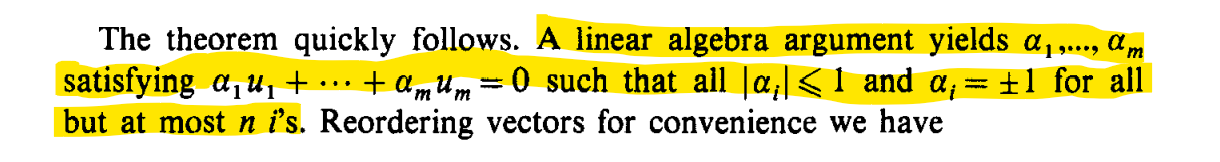
\includegraphics[scale=1.3]{Joel_Spencer_balancing_vectors.png}\retTwo\par}

Our issue was figuring out what linear algebra argument Spencer was fucking using. After thinking about it for three days while I was grading tests, I finally came up with a proof:\retTwo

\Hstatement\blab{Theorem:} Let $u_1, \ldots, u_m$ be vectors in $\mathbb{R}^n$. Then there are constants $a_1, \ldots, a_m$ satisfying\\ $a_1u_1 + \ldots + a_mu_m = 0$ such that all $|a_i| \leq 1$ and $a_i = \pm 1$ for all but at most $n$ $i$'s.

\begin{myIndent}\HexOne
	Proof:\\
	We'll proceed by an inductive argument. For our base case, let $u_{m+1} \coloneq 0$. That way\\ $\sum_{i = 1}^m 0 u_i = u_{m+1}$. Next, suppose that for $n + 1 \leq k \leq m$, we've shown that there\\ are constants $b_1, \ldots, b_{k} \in [-1, 1]$ and $\varepsilon_{k+1}, \ldots, \varepsilon_{m+1} \in \{-1, +1\}$ satisfying that:

	{\centering $b_1u_1 + \ldots + b_ku_k = \varepsilon_{k+1}u_{k+1} + \ldots + \varepsilon_{m+1}u_{m+1}$. \retTwo\par}

	If we consider the matrix $U \coloneqq \begin{bmatrix}u_1 & \cdots & u_k\end{bmatrix}$, then letting $b = (b_1, \ldots, b_k)$ we have that any $a = (a_1, \ldots, a_k) \in b + \ker(U)$ will satisfy that:
	
	{\centering $a_1u_1 + \ldots + a_{k}u_{k} = \varepsilon_{k+1}u_{k+1} + \ldots + \varepsilon_{m+1}u_{m+1}$.\retTwo\par}
	
	Since $k > n$, we know that $\ker(U)$ is nontrivial and hence unbounded. At the same time, $\|b\|_{\infty} \leq 1$. Hence, by the connectedness of $b + \ker(U)$ and the continuity of the $\infty$-norm, we know there is some $a \in b + \ker(U)$ with $\|a\|_\infty = 1$. After reordering our $u_i$, this is the same as saying that there exists $a_1, \ldots, a_{k-1} \in [-1, 1]$ and $\varepsilon_k = \pm 1$ such that:

	{\centering $a_1u_1 + \ldots + a_{k-1}u_{k-1} + \varepsilon_{k}u_k = \varepsilon_{k+1}u_{k+1} + \ldots + \varepsilon_{m+1}u_{m+1}$.\retTwo\par}
	
	Subtract both sides by $\varepsilon_{k}u_k$ to complete the induction step.\retTwo

	After induction, we will eventaully get constants $a_1, \ldots, a_n \in [-1, 1]$ and $\varepsilon_{n+1}, \ldots, \varepsilon_{m+1}$ equal to $\pm 1$ such that:

	{\centering $a_1u_1 + \ldots + a_nu_n = \varepsilon_{n+1}u_{n+1} + \ldots + \varepsilon_mu_m + \varepsilon_{m+1}u_{m+1}$. \retTwo\par}

	Move everything over to one side of the equation and forget about the $u_{m+1}$ and we have proven what we wanted.\newpage
\end{myIndent}

\dispDate{8/6/2025}\hOne

Now I'm going to go back to studying tensors.\retTwo

A \udefine{multi-index of length $k$} is a $k$-tuple $I = (i_1, \ldots, i_k)$ of integers. We say $I$ is a multi-index of $n$ if each $i$ is between $1$ and $n$. Now let $u_1, \ldots, u_n$ is a basis of $V$. For $T \in \mathcal{L}^k(V)$, write $T_I \coloneq T(u_{i_1}, \ldots, u_{i_k})$ for every multi-index $I$ of $n$ of length $k$.\retTwo

\exOne\ul{Proposition 1.3.7:} The $T_I$ uniquely determine $T$.

\begin{myIndent}\exTwoP
	Proof:\\
	When $k = 1$, $T$ is just a linear map and we've already proven this for linear maps. For $k > 1$, we proceed by induction. For each $i$, define $T_i \in L^{k-1}(V)$ by:
	
	{\centering $(v_1, \ldots, v_{k-1}) \mapsto T(v_1, \ldots, v_{k-1}, u_i)$.\retTwo\par} Then for $v = c_1u_1 + \ldots + c_nu_n$, we have:

	{\centering $T(v_1, \ldots, v_{k-1}, v) = \sum\limits_{i=1}^n c_iT_i(v_1, \ldots, v_{k-1})$\retTwo\par}

	Also, by induction each $T_i$ is uniquely determined by the coefficients $T_I$ where $I$ is a multi-index of $n$ of length $k$ with a final index equal to $i$.\retTwo

	\begin{myIndent}\exPPP
		Side note: We can see that if $C = (c_{i,j}) \in \mathcal{M}_{n \times k}(F)$ is the matrix satisfying that $v_{j} = \sum_{i=1}^n c_{i,j} u_i$ for each $j$, then:

		{\centering $T(v_1, \ldots, v_k) = \hspace{-1em}\sum\limits_{I = (i_1, \ldots, i_k)}\hspace{-0.5em} \left(\hspace{0.1em}\prod\limits_{j=1}^k c_{i_j, j}\right)T_I$ \retTwo\par}
	\end{myIndent}
\end{myIndent}

\hOne%
Given two tensors: $T_1 \in \mathcal{L}^k(V)$ and $T_2 \in \mathcal{L}^\ell(V)$, we define the \udefine{tensor product} of $T_1$ and $T_2$ as:

{\centering $(T_1 \otimes T_2)(v_1, \ldots, v_k, v_{k+1}, \ldots, v_{k + \ell}) = T_1(v_1, \ldots, v_k)T_2(v_{k + 1}, \ldots, v_{k + \ell})$\retTwo\par}

Note that:\hTwo\\ [-20pt]
\begin{itemize}
	\item $\otimes$ is associative.
	\item If $T_1$ or $T_2$ is a $0$-tensor, then $\otimes$ is just scalar multiplication.
	\item If $\lambda \in F$, $T_1 \in \mathcal{L}^k(V)$, and $T_2 \in \mathcal{L}^\ell(V)$, then $\lambda(T_1 \otimes T_2) = (\lambda T_1) \otimes T_2 = T_1 \otimes (\lambda T_2)$.
	\item If $T_1, T_2 \in \mathcal{L}^k(V)$ and $T_3 \in \mathcal{L}^\ell(V)$, then $(T_1 + T_2) \otimes T_3 = (T_1 \otimes T_3) + (T_2 \otimes T_3)$. Also $T_3 \otimes (T_1 + T_2)  = (T_3 \otimes T_1 ) + (T_3 \otimes T_2)$\retTwo
\end{itemize}

\hOne Suppose $T \in \mathcal{L}^k(V)$ and there exists $\ell_1, \ldots, \ell_k \in V^* = \mathcal{L}^1(V)$ such that $T = \ell_1 \otimes \cdots \otimes \ell_k$. Then we say $T$ is \udefine{decomposable}.\retTwo

If $u_1, \ldots, u_n$ is a basis for $V$, then we can define the \udefine{dual basis}: $u_1^*, \ldots, u_n^*$ for $V^*$ such that if $v = \sum_{i=1}^n c_iu_i$, then $u_j^*(v) = c_j$.

\begin{myIndent}\exTwoP
	To prove that this is a basis, first note that if $f \in V^*$ and $\lambda_i = f(u_i)$, then we can easily see that for any $v = \sum_{i=1}^n c_iu_i$, then:\newpage
	
	{\centering $f(v) = \sum_{i=1}^n c_if(u_i) = \sum_{i=1}^n \lambda_ic_i = \sum_{i=1}^n \lambda_iu_i^*(v)$.\retTwo\par}

	It follow that $u_1^*, \ldots, u_n^*$ span all of $V^*$. Also, consider if $f = \sum_{i=1}^n \lambda_i u_i^* = 0$ where all the $\lambda_i \in F$. Then we know that $0 = f(u_j) = \lambda_j$ for all $j$. This shows that\\ $u_1^*, \ldots, u_n^*$ are linearly  independent.\retTwo
\end{myIndent}

\pracOne\mySepTwo
Tangent: if $V, W$ are vector fields over $F$ and $A: V \to W$ is a linear map, then we define the \udefine{transpose} $A^\dag: W^* \to V^*$ of $A$ by $f \mapsto A^\dag(f) = f \circ A$.\retTwo

\exOne\ul{Claim 1.2.15:} Suppose $e_1, \ldots, e_m$ is a basis of $V$ and $u_1, \ldots, u_n$ is a basis of $W$. Then if $A = (a_{i,j})$ is the the matrix of $A$ with respect to the given bases, we have that the matrix of $A^\dag$ with respect to the dual bases of $V$ and $W$ is given by $(a_{j,i})$.

\begin{myIndent}\exTwoP
	Proof:\\
	Suppose $(c_{j,i})$ is the matrix representation of $A^\dag$. Then:

	{\centering $A^\dag(u_i^*)(e_j) = u_i^*(A(e_j)) = u_i^*(\sum_{k=1}^n a_{k,j}u_k) = a_{i,j}$ \retTwo\par}

	Simultaneously:

	{\centering $A^\dag(u_i^*)(e_j) = \sum_{k=1}^m c_{k, i} e_k^*(e_j) = c_{j, i}$ \retTwo\par}
\end{myIndent}
\pracOne\mySepTwo

\hOne Let $u_1, \ldots, u_n$ be a basis of $V$ and $u_1^*, \ldots, u_n^*$ be the corresponding dual basis of $V^*$. Then for every multi-index $I = (i_1, \ldots, i_k)$ of $n$ of length $k$, define:

{\centering $u_I^* = u_{i_1}^* \otimes \cdots \otimes u_{i_k}^*$.\retTwo\par}

Note that if $J = (j_1, \ldots, j_k)$ is another multi-index of $n$ of length $k$, then\\ $u_I^*(u_{j_1}, \ldots, u_{j_k}) = \delta_{I,J}$ where $\delta$ is the Kronecker delta function.\retTwo

\exOne\ul{Theorem 1.3.13:} The $k$-tensors $u_I^*$ form a basis for $\mathcal{L}^k(V)$.
\begin{myIndent}\exTwoP 
	Proof:\\
	Suppose $T \in \mathcal{L}^k(V)$. Then if $T^\prime \coloneq \sum_{I} T_Iu_I^*$, we have that $T^\prime_J = T_J$ for all multi-indices $J$ of $n$ of length $k$. Therefore, since $T^\prime$ and $T$ are uniquely determined by the same $T_I$, this proves that $T = T^\prime$. So, $T$ is in the span of the $u_I^*$. This proves that the $u_I^*$ span all of $\mathcal{L}^k(V)$.\retTwo

	Next suppose $T^\prime = \sum_{I} C_Iu_I^* = 0$ where each $C_I \in F$. Then if $J$ is a multi-index of $n$ of length $k$,
	
	{\centering$0 = T^\prime(u_{j_1}, \ldots, u_{j_k}) = \sum\limits_{I} C_Iu_I^*(u_{j_1}, \ldots, u_{j_k}) = C_J$\retTwo\par}

	This shows that the $u_I^*$ are linearly independent. \blacksquare\retTwo
\end{myIndent}

\ul{Corollary 1.3.15:} If $V$ is an $n$-dimensional vector space, then $\mathcal{L}^k(V)$ is an\\ $n^k$-dimensional vector space.\newpage

\hOne If $V, W$ are vector fields over $F$, $A: V \to W$ is a linear map, and $T \in \mathcal{L}^k(W)$, we define $A^\dag T(v_1, \ldots, v_k) \coloneq T(Av_1, \ldots, Av_k)$.\retTwo

We call $A^\dag T$ the \udefine{pullback} of $T$ by the map $A$. Note that this is just a generalization of taking the transpose of $A$.\retTwo

\exOne\ul{Proposition 1.3.18:} If we denote $A^\dag : \mathcal{L}^k(W) \to \mathcal{L}^k(V)$ to be the map $T \mapsto A^\dag T$, then $A^\dag$ is a linear map.

\begin{myIndent}\exTwoP This should be pretty obvious\dots\retTwo
\end{myIndent}

Furthermore, $A^\dag(T_1 \otimes T_2) = (A^\dag T_1) \otimes (A^\dag T_2)$.

\begin{myIndent}\exTwoP
	Proof:\\
	Suppose $T_1 \in \mathcal{L}^k(V)$ and $T_2 \in \mathcal{L}^\ell(V)$. Then:

	{\centering\begin{tabular}{l}
		$A^\dag(T_1 \otimes T_2)(v_1, \ldots, v_k, v_{k+1}, \ldots, v_{k+\ell})$\\
		$\phantom{aaaaaaaaaaaaaa} = (T_1 \otimes T_2)(Av_1, \ldots, Av_k, Av_{k+1}, \ldots, Av_{k+\ell})$\\
		$\phantom{aaaaaaaaaaaaaa} = T_1(Av_1, \ldots, Av_k)T_2(Av_{k+1}, \ldots, Av_{k+\ell})$\\
		$\phantom{aaaaaaaaaaaaaa} = A^\dag T_1(v_1, \ldots, v_k)A^\dag T_2(v_{k+1}, \ldots, v_{k+\ell})$\\
		$\phantom{aaaaaaaaaaaaaa} = (A^\dag T_1 \otimes A^\dag T_2)(v_1, \ldots, v_k, v_{k+1}, \ldots, v_{k+\ell})$. $\blacksquare$
	\end{tabular}\retTwo\par}
\end{myIndent}

As a corollary to the above fact, we know that pullbacks map decomposable tensors to decomposable tensors.\retTwo

Finally, suppose $B: U \to V$ is another linear map. Then $(AB)^\dag T = B^\dag(A^\dag T)$ for all $T \in \mathcal{L}^k(W)$. In other words, $(AB)^\dag = B^\dag A^\dag$.

\begin{myIndent}\exTwoP
	Proof:

	{\centering\begin{tabular}{l}
		$B^\dag(A^\dag T)(v_1, \ldots, v_k) = A^\dag T(Bv_1, \ldots, Bv_k)$\\
		$\phantom{B^\dag(A^\dag T)(v_1, \ldots, v_k)} = T(ABv_1, \ldots, ABv_k) = (AB)^\dag T(v_1, \ldots, v_k)$. $\blacksquare$
	\end{tabular}\retTwo\par}
\end{myIndent}

\hOne\blab{Alternating $k$-Tensors:}\\
Let $V$ be an $n$-dimensional vector space over a field $F$ with characteristic $\neq 2$ and $S_k$ be the symmetric group over $\{1, \ldots, k\}$. For $\sigma \in S_k$ and $T \in \mathcal{L}^k(V)$, we define $T^\sigma \in \mathcal{L}^k(V)$ by:

{\centering $T^\sigma(v_1, \ldots, v_k) = T(v_{\sigma^{-1}(1)}, \ldots, v_{\sigma^{-1}(k)})$ \retTwo\par}

\exOne\ul{Proposition 1.4.14:}
\begin{itemize}
	\item[(a)] If $T = \ell_1 \otimes \cdots \otimes \ell_k$ where each $\ell_i \in V^*$, then $T^\sigma = \ell_{\sigma(1)} \otimes \cdots \otimes \ell_{\sigma(k)}$.
	
	\begin{myIndent}\exTwoP
		Proof:

		{\centering\begin{tabular}{l}
			$T^\sigma(v_1, \ldots, v_k) = T(v_{\sigma^{-1}(1)}, \ldots, v_{\sigma^{-1}(k)}) = \ell_1(v_{\sigma^{-1}(1)}) \cdots \ell_k(v_{\sigma^{-1}(k)})$\\
			$\phantom{T^\sigma(v_1, \ldots, v_k) = T(v_{\sigma^{-1}(1)}, \ldots, v_{\sigma^{-1}(k)})} = \ell_{\sigma(1)}(v_1) \cdots \ell_{\sigma(k)}(v_k)$\\
			$\phantom{T^\sigma(v_1, \ldots, v_k) = T(v_{\sigma^{-1}(1)}, \ldots, v_{\sigma^{-1}(k)})} = (\ell_{\sigma(1)} \otimes \cdots \otimes \ell_{\sigma(k)})(v_1, \ldots, v_k)$
		\end{tabular}\retTwo\par}
	\end{myIndent}

	\item[(b)] If $\sigma \in S_k$, the function $T \mapsto T^\sigma$ is a linear map from $\mathcal{L}^k(V)$ to $\mathcal{L}^k(V)$.
	\begin{myIndent}\exTwoP
		This should be obvious. Also note that this map is invertible via the function $T \mapsto T^{(\sigma^{-1})}$.\newpage
	\end{myIndent}

	\item[(c)] If $\sigma, \tau \in S_k$, then $(T^\sigma)^\tau = T^{\sigma \tau}$.
	
	\begin{myIndent}\exTwoP
		Proof:\\
		Let $u_i \coloneq v_{\tau^{-1}(i)}$ for all $i$. Then:

		{\centering\begin{tabular}{l}
			$(T^\sigma)^\tau(v_1, \ldots, v_k) = T^\sigma(v_{\tau^{-1}(1)}, \ldots, v_{\tau^{-1}(k)})$\\ [2pt]

			$\phantom{(T^\sigma)^\tau(v_1, \ldots, v_k)} = T^\sigma(u_1, \ldots, u_k) = T(u_{\sigma^{-1}(1)}, \ldots, u_{\sigma^{-1}(k)})$\\ [2pt]

			$\phantom{(T^\sigma)^\tau(v_1, \ldots, v_k) = T^\sigma(u_1, \ldots, u_k)} = T(v_{\tau^{-1}(\sigma^{-1}(1))}, \ldots, v_{\tau^{-1}(\sigma^{-1}(k))})$\\ [2pt]

			$\phantom{(T^\sigma)^\tau(v_1, \ldots, v_k) = T^\sigma(u_1, \ldots, u_k)} = T(v_{(\sigma\tau)^{-1}(1)}, \ldots, v_{(\sigma\tau)^{-1}(k)})$\\ [2pt]

			$\phantom{(T^\sigma)^\tau(v_1, \ldots, v_k) = T^\sigma(u_1, \ldots, u_k)} = T^{\sigma\tau}(v_1, \ldots, v_k)$
		\end{tabular}\retTwo\par}
	\end{myIndent}
\end{itemize}

\hOne Let $V$ be a vector space and $k \geq 1$ be an integer. Then $T \in \mathcal{L}^k(V)$ is \udefine{alternating} if $T^\sigma = \sgn(\sigma)T$ for all $\sigma \in S_k$. We denote $\mathcal{A}^k(V)$ as the set of all alternating\\ $k$-tensors on $V$.

\begin{myIndent}\hTwo
	Note:
	\begin{itemize}
		\item If $c_1, c_2 \in F$ and $T_1, T_2 \in \mathcal{A}^k(V)$, then since $T \mapsto T^\sigma$ is a linear map, we have for all $\sigma \in S_k$ that:
		
		{\centering\begin{tabular}{l}
			$(c_1T_1 + c_2T_2)^{\sigma} = c_1T_1^{\sigma} + c_2T_2^\sigma$\\
			$\phantom{(c_1T_1 + c_2T_2)^{\sigma}} = c_1\sgn(\sigma)T_1 + c_2\sgn(\sigma)T_2 = \sgn(\sigma)(c_1T_1 + c_2T_2)$
		\end{tabular}\retTwo\par}

		This proves that $\mathcal{A}^k(V)$ is a subspace of $\mathcal{L}^k(V)$.\retTwo

		\item We shall define $\mathcal{A}^0(V) \coloneqq \mathcal{L}^0(V) = F$.\retTwo
	\end{itemize}
\end{myIndent}

Given an integer $k > 0$, and a tensor $T \in \mathcal{L}^k(V)$, let:

{\centering $\Alt(T) \coloneqq \sum\limits_{\tau \in S_k} \sgn(\tau)T^\tau$.\retTwo\par}

Then the \udefine{alternation operation} has the following properties:\\
\exOne\ul{Proposition 1.4.17:}
\begin{itemize}
	\item[(a)] Given any $T \in \mathcal{L}^k(V)$ and $\sigma \in S_k$ (where $k > 0$), we have that\\ $(\Alt(T))^{\sigma} = \sgn(\sigma)\Alt(T)$. I.e., $\Alt(T)$ is an alternating tensor.
	
	\begin{myIndent}\exTwoP
		Proof:\\
		By proposition 1.4.14 plus the fact that $(\sgn(\sigma))^2 = 1$, we have that:

		{\centering\begin{tabular}{l}
			$(\Alt(T))^\sigma = (\sum\limits_{\tau \in S_k}\sgn(\tau)T^{\tau})^{\sigma}$\\ [16pt]
		
			$\phantom{(\Alt(T))^\sigma} = 1 \cdot \hspace{-0.4em}\sum\limits_{\tau \in S_k}\sgn(\tau)T^{\tau\sigma} = (\sgn(\sigma))^2 \sum\limits_{\tau \in S_k}\sgn(\tau)T^{\tau\sigma}$\\ [16pt]

			$\phantom{(\Alt(T))^\sigma = 1 \cdot \hspace{-0.4em}\sum\limits_{\tau \in S_k}\sgn(\tau)T^{\tau\sigma}} = \sgn(\sigma) \sum\limits_{\tau \in S_k}\sgn(\tau\sigma)T^{\tau\sigma} = \sgn(\sigma) \sum\limits_{\tau^\prime \in S_k}\sgn(\tau^\prime)T^{\tau^\prime}$\\ [16pt]

			$\phantom{(\Alt(T))^\sigma = 1 \cdot \hspace{-0.4em}\sum\limits_{\tau \in S_k}\sgn(\tau)T^{\tau\sigma} = \sgn(\sigma) \sum\limits_{\tau \in S_k}\sgn(\tau\sigma)T^{\tau\sigma}} = \sgn(\sigma) \Alt(T)$\\ [16pt]
		\end{tabular} \newpage\par}
	\end{myIndent}

	\item[(b)] If $T \in \mathcal{A}^k(V)$, the $\Alt(T) = k!T$.
	
	\begin{myIndent}\exTwoP
		Proof:\\
		Since $T^\tau = \sgn(\tau)T$ for all $\tau \in S_k$, we know:

		{\centering\begin{tabular}{l}
			$\Alt(T) = \sum\limits_{\tau \in S_k} \sgn(\tau)T^\tau = \sum\limits_{\tau \in S_k} (\sgn(\tau))^2T = \sum\limits_{\tau \in S_k} (1)T = |S_k|T = k!T$
		\end{tabular} \retTwo\par}
	\end{myIndent}

	\item[(c)] $\Alt(T^\sigma) = (\Alt(T))^\sigma$.
	
	\begin{myIndent}\exTwoP
		Proof:\\
		By similar reasoning to in part (a), we have that:

		{\centering\begin{tabular}{l}
			$\Alt(T^\sigma) = 1 \cdot \hspace{-0.4em}\sum\limits_{\tau \in S_k} \sgn(\tau) T^{\sigma\tau} = (\sgn(\sigma))^2 \sum\limits_{\tau \in S_k} \sgn(\tau) T^{\sigma\tau}$\\ [12pt]

			$\phantom{\Alt(T^\sigma) = 1 \cdot \hspace{-0.4em}\sum\limits_{\tau \in S_k} \sgn(\tau) T^{\sigma\tau}} = \sgn(\sigma) \sum\limits_{\tau \in S_k} \sgn(\sigma\tau) T^{\sigma\tau}$\\ [12pt]

			$\phantom{\Alt(T^\sigma) = 1 \cdot \hspace{-0.4em}\sum\limits_{\tau \in S_k} \sgn(\tau) T^{\sigma\tau}} = \sgn(\sigma) \sum\limits_{\tau^\prime \in S_k} \sgn(\tau^\prime) T^{\tau^\prime} = \sgn(\sigma)\Alt(T)$
		\end{tabular} \retTwo\par}

		And since $\sgn(\sigma)\Alt(T) = (\Alt(T))^\sigma$ by part (a), we know $\Alt(T^\sigma) = (\Alt(T))^\sigma$.\retTwo
	\end{myIndent}

	\item[(d)] The map $\Alt: \mathcal{L}^k(V) \to \mathcal{L}^k(V)$ defined by $T \mapsto \Alt(T)$ is a linear map. (Also it's onto if $F$ has characteristic $0$ or $> k$.)
	
	\begin{myIndent}\exTwoP
		Proof:\\
		$\Alt$ is a linear map because it is a linear combination of a bunch of linear maps. The onto property follows from part (b).\retTwo
	\end{myIndent}
\end{itemize}

\hOne\dispDate{8/7/2025}

If $I = (i_1, \ldots, i_k)$ is a multi-index of $n$ of length $k$, then we write:
\begin{itemize}
	\item $I$ is \udefine{repeating} if $i_s = i_r$ for some $s \neq r$.
	\item $I$ is \udefine{increasing} if $i_1 < i_2 < \ldots < i_k$.
	\item Given $\sigma \in S_k$, we define $I^\sigma = (i_{\sigma(1)}, \ldots, i_{\sigma(k)})$.\retTwo
\end{itemize}

Note that if $I$ is not repeating, then there is a unique permutation $\sigma \in S_k$ such that $I^\sigma$ is increasing.\retTwo

Let $u_1, \ldots, u_n$ be a basis of the vector space $V$ over a field $F$ of characteristic $\neq 2$, and let $u_1^*, \ldots, u_n^*$ be the corresponding dual basis. Now given the multi-index\\ $I = (i_1, \ldots, i_k)$, set $u_I^* = u_{i_1}^* \otimes \cdots \otimes u_{i_k}^*$. Next define $\Psi_I = \Alt(u_I^*)$.\retTwo

\exOne\ul{Proposition 1.4.20:} Let $I = (i_1, \ldots, i_k)$ and $J = (j_1, \ldots, j_k)$ be multi-indices.
\begin{itemize}
	\item[(a)] $\Psi_{I^\sigma} = \sgn(\sigma)\Psi_I$.
	\begin{myIndent}\exTwoP
		To start off, by the last proposition:
		
		{\centering$\sgn(\sigma)\Psi_I = \sgn(\sigma)\Alt(u_I^*) = (\Alt(u_I^*))^\sigma = \Alt((u_I^*)^\sigma)$.\newpage\par}

		Next, set $\ell_j = u^*_{i_j}$ for $1 \leq j \leq k$. Then by proposition 1.4.14, we have:
		
		{\centering$(u_I^*)^\sigma = (\ell_1 \otimes \cdots \otimes \ell_k)^\sigma = \ell_{\sigma(1)} \otimes \cdots \otimes \ell_{\sigma(k)} = u_{i_{\sigma(1)}}^* \otimes \cdots \otimes u_{i_{\sigma(k)}}^* = u^*_{I^\sigma}$.\retTwo\par}

		Thus $\sgn(\sigma)\Psi_I = \Alt((u_I^*)^\sigma) = \Alt(u^*_{I^\sigma}) = \Psi_{I^\sigma}$.\retTwo
	\end{myIndent}

	\item[(b)] If $I$ is repeating, $\Psi_{I} = 0$.
	
	\begin{myIndent}\exTwoP
		If $I$ is repeating, then there exists $r \neq s$ such that $i_r = i_s$. Then in turn, if $\tau_{r,s} \in S_k$ is the transposition of $r$ and $s$, then $\sgn(\tau_{r,s}) = -1$ and $I^{\tau_{r,s}} = I$. Then by part (a), we have:

		{\centering$\Psi_I = \Psi_{I^{\tau_{r,s}}} = \sgn(\tau_{r,s})\Psi_{I} = -\Psi_{I}$\retTwo\par}
		
		This is only possible if $\Psi_I(v_1, \ldots, v_k) = 0$ for all $v_1, \ldots, v_k \in V$. Hence $\Psi_I$ is the zero map.\retTwo
	\end{myIndent}


	\item[(c)] If $I$ and $J$ are strictly increasing, then $\Psi_I(u_{j_1}, \ldots, u_{j_k}) = \delta_{I,J}$ where $\delta$ is the Kronecker delta function.
	
	\begin{myIndent}\exTwoP
		To start off, note that:

		{\centering\begin{tabular}{l}
			$\Psi_I(u_{j_1}, \ldots, u_{k_k}) = \sum\limits_{\tau \in S_k}\sgn(\tau)(u_I^*)^{\tau}(u_{j_1}, \ldots, u_{j_k})$\\ [18pt]

			$\phantom{\Psi_I(u_{j_1}, \ldots, u_{k_k})} = \sum\limits_{\tau \in S_k}\sgn(\tau)(u_{i_1}^* \otimes \cdots \otimes u_{i_k}^*)^{\tau}(u_{j_1}, \ldots, u_{j_k})$\\ [18pt]

			$\phantom{\Psi_I(u_{j_1}, \ldots, u_{k_k})} = \sum\limits_{\tau \in S_k}\sgn(\tau)(u_{i_{\tau(1)}}^* \otimes \cdots \otimes u_{i_{\tau(k)}}^*)(u_{j_1}, \ldots, u_{j_k})$\\ [18pt]

			$\phantom{\Psi_I(u_{j_1}, \ldots, u_{k_k})} = \sum\limits_{\tau \in S_k}\sgn(\tau)u_{i_{\tau(1)}}^*(u_{j_1})\cdots u_{i_{\tau(k)}}^*(u_{j_k})$\\ [18pt]
		\end{tabular}\retTwo\par}

		Now it's clear that $u_{i_{\tau(1)}}^*(u_{j_1})\cdots u_{i_{\tau(k)}}^*(u_{j_k}) = \delta_{I^\tau, J}$. Also, since both $J$ and $I$ are strictly increasing and also since there is only one permutation such that $I^\sigma$ is strictly increasing for any nonrepeating $I$, we know that $\delta_{I^\tau, J} = 1$ iff $\tau = \myId$ and $I = J$. And in that case $\sgn(\tau) = 1$. Hence: 
		
		{\centering $\sum\limits_{\tau \in S_k}\sgn(\tau)u_{i_{\tau(1)}}^*(u_{j_1})\cdots u_{i_{\tau(k)}}^*(u_{j_k}) = \delta_{I,J}$.\retTwo\par}
	\end{myIndent}
\end{itemize}

\ul{Proposition 1.4.24:} Suppose $F$ has characteristic $0$ or greater than $k$. Then\\ $\{\Psi_J : J \text{ is increasing}\}$ is a basis for $\mathcal{A}^k(V)$.

\begin{myIndent}\exTwoP
	Proof:\\
	Suppose $T \in \mathcal{A}^k(V)$. By theorem 1.3.13, we know there exists $a_I \in F$ such that $T = \sum_{I} a_I u_I^*$. However, we also know that $k!T = \Alt(T)$. Since $\Alt$ is a linear map, we thus know that:

	{\centering $T = \frac{1}{k!}\Alt(T) = \sum\limits_I \frac{a_I}{k!} \Alt(u_I^*) = \sum\limits_I \frac{a_I}{k!} \Psi_I$\newpage\par}

	If $I$ is repeating, then $\frac{a_I}{k!} \Psi_I^*$  cancels. Otherwise, there is some $\sigma \in S_k$ and some increasing multi-index $J$ such that:
	
	{\centering $\frac{a_I}{k!} \Psi_I = \frac{a_I}{k!} \Psi_{J^\sigma} = \frac{a_I\sgn(\sigma)}{k!} \Psi_{J}$.\retTwo\par}

	By collecting terms, we get that $T = \hspace{-1em}\sum\limits_{J \text{ increasing}}\hspace{-1em}c_J\Phi_J$ where each $c_J \in F$.\retTwo

	This shows that the $\Psi_J$ span all of $\mathcal{A}^k(V)$. Next we show that they form a basis.\\ Suppose $T = \hspace{-1em}\sum\limits_{J \text{ increasing}}\hspace{-1em}c_J\Phi_J = 0$.\retTwo

	Then by part (c) of the last proposition, we know that if $I = (i_1, \ldots, i_k)$ is an\\ increasing multi-index, then:

	{\centering $0 = T(u_{i_1}, \ldots, u_{i_k}) = C_I$ \retTwo\par}

	So, all the $C_I$ are equal to $0$. $\blacksquare$\retTwo
\end{myIndent}

\ul{Corollary:} If $F$ has characteristic $0$ or greater than $k$, then $\mathcal{A}^k(V)$ has dimension $\binom{n}{k}$.\retTwo

\ul{Corollary 2:} If $F$ has characteristic $0$ or greater than $k \geq n$, then any alternating $n$-tensor on $V$ is a scalar multiple of the determinant function. Also, there are no nontrivial alternating $m$-tensors where $n < m \leq k$.\retTwo

\pracOne\ul{Exercise 1.4.ix:} Suppose $A: V \to W$ is a linear map. Then if $T \in \mathcal{A}^k(W)$, we have that $A^\dag T \in \mathcal{A}^k(V)$. Hence, the pullback operation maps alternating tensors to alternating tensors.

\begin{myIndent}\pracTwo
	Proof:\\
	Suppose $\sigma \in S_k$. Then for any $v_1, \ldots, v_k \in V$, we have that:

	{\centering\begin{tabular}{l}
		$(A^\dag T)^\sigma(v_1, \ldots, v_k) = A^\dag T(v_{\sigma^{-1}(1)}, \ldots, v_{\sigma^{-1}(k)})$\\ [6pt]

		$\phantom{(A^\dag T)^\sigma(v_1, \ldots, v_k)} = T(Av_{\sigma^{-1}(1)}, \ldots, Av_{\sigma^{-1}(k)})$\\ [6pt]

		$\phantom{(A^\dag T)^\sigma(v_1, \ldots, v_k)} = T^\sigma(Av_1, \ldots, Av_k)$\\ [6pt]

		$\phantom{(A^\dag T)^\sigma(v_1, \ldots, v_k)} = \sgn(\sigma)T(Av_1, \ldots, Av_k) = \sgn(\sigma)A^\dag T(v_1, \ldots, v_k)$
	\end{tabular}\retTwo\par}

	Hence, $(A^\dag T)^\sigma = \sgn(\sigma)A^\dag T$. This proves that $A^\dag T$ is alternating. $\blacksquare$\retTwo
\end{myIndent}

\ul{Exercise 1.4.x:} Additionally to the last exercise, we have that if $T \in \mathcal{L}^k(V)$, then\\ $A^\dag(\Alt(T)) = \Alt(A^\dag T)$.

\begin{myIndent}\pracTwo
	Proof:\\
	If $v_1, \ldots, v_k \in V$, then:

	{\centering\begin{tabular}{l}
		$\Alt(A^\dag T)(v_1, \ldots, v_k) = \sum\limits_{\tau \in S_k}\sgn(\tau)(A^\dag T )^\tau(v_1, \ldots, v_k)$\\ [16pt]

		$\phantom{\Alt(A^\dag T)(v_1, \ldots, v_k)} = \sum\limits_{\tau \in S_k}\sgn(\tau)A^\dag T(v_{\tau^{-1}(1)}, \ldots, v_{\tau^{-1}(k)})$\\ [16pt]

		$\phantom{\Alt(A^\dag T)(v_1, \ldots, v_k) } = \sum\limits_{\tau \in S_k}\sgn(\tau)T(Av_{\tau^{-1}(1)}, \ldots, Av_{\tau^{-1}(k)})$\\ [-24pt]

		$\phantom{\Alt(A^\dag T)(v_1, \ldots, v_k) = \Alt(T)(Av_1, \ldots, Av_k) = A^\dag(\Alt (T))(v_1, \ldots, v_k)}$
	\end{tabular}\newpage
	
	\begin{tabular}{l}
		$\phantom{\Alt(A^\dag T)(v_1, \ldots, v_k)} = \sum\limits_{\tau \in S_k}\sgn(\tau)T^\tau(Av_1, \ldots, Av_k)$\\ [16pt]

		$\phantom{\Alt(A^\dag T)(v_1, \ldots, v_k) } = \Alt(T)(Av_1, \ldots, Av_k) = A^\dag(\Alt (T))(v_1, \ldots, v_k)$
	\end{tabular}\retTwo\par}

	This shows that $\Alt(A^\dag T) =  A^\dag(\Alt (T))$. $\blacksquare$\retTwo
\end{myIndent}

\hOne\blab{The space $\Lambda^k(V^*)$:}\\
If $k > 1$, a decomposable $k$-tensor $\ell_1 \otimes \cdots \otimes \ell_k$ with each $\ell_i \in V^*$ is called \udefine{redundant} if $\ell_i = \ell_{i+1}$ for some index $i$. We let $\mathcal{I}^k(V)$ be the span of all redundant $k$-tensors.

\begin{myIndent}\hTwo 
	If $k = 1$, we define $\mathcal{I}^1(V) \coloneq \{0\} \subseteq \mathcal{L}^1(V)$.\\ Also if $k = 0$, we define $\mathcal{I}^0(V) \coloneq \{0\} \subseteq F$.\retTwo 
\end{myIndent}

\exOne\ul{Proposition 1.5.2:} Suppose $F$ has characteristic $\neq 2$. If $T \in \mathcal{I}^k(V)$, then $\Alt(T) = 0$. In other words, $\mathcal{I}^k(V) \subseteq \ker(\Alt)$.

\begin{myIndent}\exTwoP
	Proof:\\
	If $T \in \mathcal{I}^k(V)$, then we know there are redundant decomposable $k$-tensors\\ $T_1, \ldots, T_m$ as well as scalars $c_1, \ldots, c_m \in F$ such that $T = \sum_{j=1}^m c_jT_j$. Then since\\ $\Alt(T) = \sum_{j=1}^m c_j\Alt(T_j)$, all we need to do now is show that $\Alt(T_j) = 0$ for\\ every $j$.\retTwo

	Since $T_j$ is a redundant decomposable $k$-tensor, we know that $T_j = \ell_1 \otimes \cdots \otimes \ell_k$ where $\ell_i = \ell_{i+1}$ for some $1 \leq i < k$. In turn, if $\tau_{i, i+1} \in S_k$ is the transposition of $i$ and $i+1$, we have that $(T_j)^{\tau_{i,i+1}} = T_j$ and $\sgn(\tau_{i, i+1}) = -1$. Hence:

	{\centering$\Alt(T_j) = \Alt((T_j)^{\tau_{i, i+1}}) = \sgn(\tau_{i,i+1})\Alt(T_j) = -\Alt(T_j)$\retTwo\par}

	This implies that $\Alt(T_j) = 0$. $\blacksquare$\retTwo
\end{myIndent}

\ul{Proposition 1.5.3:} If $T \in \mathcal{I}^r(V)$ and $T^\prime \in \mathcal{L}^s(V)$, then $T \otimes T^\prime$ and $T^\prime \otimes T$ are in $\mathcal{I}^{r+s}(V)$.

\begin{myIndent}\exTwoP
	Proof:\\
	The argument for $T^\prime \otimes T$ being in $\mathcal{I}^{r+s}(V)$ is mostly identical to the argument for $T \otimes T^\prime$  being in $\mathcal{I}^{r+s}(V)$. So, I'll focus only on proving the latter.\retTwo

	To start off, like before we know that there are redundant decomposable $r$-tensors $T_1, \ldots, T_m$ as well as scalars $c_1, \ldots, c_m \in F$ such that $T = \sum_{j=1}^m c_jT_j$. Hence, it suffices to show that $T_j \otimes T^\prime \in \mathcal{I}^{r+s}(V)$ for all $1 \leq j \leq m$ since:

	{\center$T \otimes T^\prime = (\sum_{j=1}^m c_jT_j) \otimes T^\prime = \sum_{j=1}^m c_j (T_j \otimes T^\prime)$\retTwo\par}

	Fortunately, by writing $T^\prime = \sum_{I} d_Iu_I^*$, we can see that:

	{\centering $T_j \otimes T^\prime = T_j \otimes (\sum\limits_{I} d_I u_I^*) = \sum\limits_{I} d_I(T_j \otimes u_I^*)$\retTwo\par}

	Now since both $u_I^*$ and $T_j$ are decomposable and $T_j$ is redundant, we can easily see that $T_j \otimes u_I^*$ is decomposable and redundant. It follows that $T_j \otimes T^\prime \in \mathcal{I}^{r+s}(V)$. $\blacksquare$\retTwo
\end{myIndent}

\ul{Proposition 1.5.4:} Suppose $F$ has characteristic $\neq 2$. If $T \in \mathcal{L}^k(V)$ and $\sigma \in S_k$, then $T^\sigma = \sgn(\sigma)T + S$ where $S \in \mathcal{I}^k(V)$.\newpage

\begin{myIndent}\exTwoP
	Proof:\\
	Hopefully you're getting use to this trick. It suffices to assume $T$ is decomposable. After all, after writing $T = \sum_{I} c_Iu_I^*$, if we can show for all multi-indexes $I$ that $(u_{I}^*)^\sigma = \sgn(\sigma)u_{I}^* + S_I$ where $S_I \in \mathcal{I}^k(V)$, then we can set $S = \sum_{I} c_I S_I \in \mathcal{I}^k(V)$ and have that:

	{\centering $T^\sigma = \sum\limits_{I} c_I (u_I^*)^\sigma = \sgn(\sigma)\sum\limits_{I} c_I u_I^* + \sum\limits_{I} S_I = \sgn(\sigma)T + S$\retTwo\par}
	
	So suppose $T = \ell_1 \otimes \cdots \otimes \ell_k$. Then given $\sigma \in S^k$, we can write $\sigma = \tau_1 \ldots \tau_m$ as the product of $m$ many transpositions of adjacent pairs of numbers in $\{1, \ldots, k\}$.
	\begin{myIndent}\exPPP
		(by adjacent I mean a pair $\{j, j+1\}$ where $1 \leq j < k$\dots)\retTwo
	\end{myIndent}

	We shall induct on $m$. First assume $m = 1$. Thus $\sigma = \tau_{j,j+1}$ for some $1 \leq j < k$ and hence $\sgn(\sigma) = -1$. Also:

	{\centering\begin{tabular}{l}
		$T^\sigma -\sgn(\sigma)T = T^\sigma + T$\\ [3pt]

		$\phantom{T^\sigma -\sgn(\sigma)T} = (\ell_1 \otimes \cdots \otimes \ell_{j-1} \otimes \ell_{j+1} \otimes \ell_{j} \otimes \ell_{j+2} \otimes \cdots \otimes \ell_{k}) + (\ell_1 \otimes \cdots \otimes \ell_k)$\\ [3pt]

		$\phantom{T^\sigma -\sgn(\sigma)T} = (\ell_1 \otimes \cdots \otimes \ell_{j-1}) \otimes \left((\ell_{j+1} \otimes \ell_j) + (\ell_j \otimes \ell_{j+1})\right) \otimes (\ell_{j+2} \otimes \cdots \otimes \ell_{k})$
	\end{tabular}\retTwo\par}

	Now note that:

	{\centering\begin{tabular}{l}
		$(\ell_{j} + \ell_{j+1}) \otimes (\ell_{j} + \ell_{j+1}) = (\ell_j \otimes \ell_j) + (\ell_j \otimes \ell_{j+1}) + (\ell_{j+1} \otimes \ell_j) + (\ell_{j+1} \otimes \ell_{j+1})$.
	\end{tabular}\retTwo\par}

	Therefore:

	{\centering\begin{tabular}{l}
		$T^\sigma - \sgn(\sigma)T = (\ell_1 \otimes \cdots \otimes \ell_{j-1}) \otimes (\ell_j + \ell_{j+1}) \otimes (\ell_j + \ell_{j+1}) \otimes (\ell_{j+1} \otimes \cdots \otimes \ell_{k})$\\
		$\phantom{T^\sigma - \sgn(\sigma)T = aaaaaaaaaaa} - (\ell_1 \otimes \cdots \otimes \ell_{j-1}) \otimes \ell_j \otimes \ell_j \otimes (\ell_{j+2} \otimes \cdots \otimes \ell_{k})$\\
		$\phantom{T^\sigma - \sgn(\sigma)T = aaaaaaaaaaa} - (\ell_1 \otimes \cdots \otimes \ell_{j-1}) \otimes \ell_{j+1} \otimes \ell_{j+1} \otimes (\ell_{j+2} \otimes \cdots \otimes \ell_{k})$\\
	\end{tabular}\retTwo\par}

	Hence $T^\sigma - \sgn(\sigma)T \in \mathcal{I}^k(V)$ and we are done with this case.\retTwo

	Now suppose $m > 1$. Then $\sigma = \tau_{j,j+1} \sigma^\prime$ where $\sigma^\prime$ is the product of $m-1$\\ transpositions. By induction, we know that there exists $S_1 \in \mathcal{I}^k(V)$ such that:

	{\centering $T^\sigma = (T^{\tau_{j,j+1}})^{\sigma^\prime} = \sgn(\sigma^\prime)T^{\tau_{j,j+1}} + S_1$ \retTwo\par}

	Also by our base case, there is $S_2 \in \mathcal{I}^k(V)$ such that $T^{\tau_{j,j+1}} = \sgn(\tau_{j,j+1})T + S_2$. Then setting $S = \sgn(\tau_{j,j+1})S_2 + S_1$, we have that $S \in \mathcal{I}^K(V)$ and:

	{\centering $T^\sigma = \sgn(\sigma^\prime)(\sgn(\tau_{j,j+1})T + S_2) + S_1 = \sgn(\sigma)T + S$. $\blacksquare$\retTwo\par}
\end{myIndent}

\ul{Corollary 1.5.6:} Suppose $F$ has characteristic $\neq 2$. If $T \in \mathcal{L}^k(V)$, then\\ $\Alt(T) = k!T + S$ where $S \in \mathcal{I}^k(V)$.

\begin{myIndent}\exTwoP
	Proof:\\
	Given any $\tau \in S_k$, let $S_\tau \in \mathcal{I}^k(V)$ be such that $T^\tau = \sgn(\tau) T + S_\tau$. Then\\ $S \coloneq \sum_{\tau \in S_k} \sgn(\tau)S_\tau \in \mathcal{I}^k(V)$ and:

	{\center $\Alt(T) = \sum\limits_{\tau \in S_k}\sgn(\tau)T^\tau = \sum\limits_{\tau \in S_k} (\sgn(\tau))^2 T + \sum\limits_{\tau \in S_k} \sgn(\tau)S_{\tau} = k!T + S$. $\blacksquare$ \retTwo\par}
\end{myIndent}

\ul{Corollary 1.5.8:} Let $k \geq 1$. Then let $V$ be a vector space over a field $F$ of\\ characteristic $0$ or $> \max(k, 2)$. Then:

{\centering $\mathcal{I}^k(V) = \ker(\Alt: \mathcal{L}^k(V) \to \mathcal{A}^k(V))$ \retTwo\par}

\begin{myIndent}\exTwoP
	Proof:\\
	We already know from proposition 1.5.2 that $\mathcal{I}^k(V) \subseteq \ker(\Alt)$. To prove the\\ reverse relation, suppose $T \in \mathcal{L}^k(V)$ satisfies that $\Alt(T) = 0$. Then based on the previous corollary, we know there exists $S \in \mathcal{I}^k(V)$ such that $-\frac{1}{k!}S = T - \Alt(T)$. Hence $T \in \mathcal{I}^k(V)$. $\blacksquare$\retTwo
\end{myIndent}

\ul{Theorem 1.5.9:} Suppose $F$ is a field of characteristic $0$ or $> \max(k, 2)$. Then any element $T \in \mathcal{L}^k(V)$ can be written uniquely as a sum $T_1 + T_2$ where $T_1 \in \mathcal{A}^k(V)$ and $T_2 \in \mathcal{I}^k(V)$. I.e, $\mathcal{L}^k(V) = \mathcal{A}^k(V) \oplus \mathcal{I}^k(V)$.

\begin{myIndent}\exTwoP
	Proof:\\
	Let $W \in \mathcal{I}^k(V)$ satisfy that $\Alt(T) = k!T + W$. Then set $T_1 = \frac{1}{k!}\Alt(T)$ and\\ $T_2 = -\frac{1}{k!}W$. Then clearly $T = T_1 + T_2$ with $T_1 \in \mathcal{A}^k(V)$ and $T_2 \in \mathcal{I}^k(V)$.\retTwo

	Next, to prove uniqueness suppose $T^\prime_1 + T^\prime = T$ with $T^\prime_1 \in \mathcal{A}^k(V)$ and $T^\prime_2 \in \mathcal{I}^k(V)$. Then $T_1 - T^\prime_1 \in \mathcal{A}^k(V)$, $T_2 - T^\prime_2 \in \mathcal{I}^k(V)$, and $(T_1 - T^\prime_1) + (T_2 - T_2^\prime) = 0$. So:

	{\center $0 = \Alt(0) = \Alt((T_1 - T^\prime_1) + (T_2 - T_2^\prime)) = k!(T_1 - T^\prime_1)$ \retTwo\par}

	Hence $T_1 = T^\prime_1$ and it easily follows $T_2 = T^\prime_2$. $\blacksquare$\retTwo
\end{myIndent}

\hOne Let $k \geq 0$. Let $V$ be a finite dimensional vector space over a field $F$ of characteristic $0$ or $> \max(k, 2)$. Then we define:

{\centering $\Lambda^k(V^*) \coloneq \mathcal{L}^k(V) / \mathcal{I}^k(V)$ \retTwo\par}

By the first isomorphism theorem along with the previous theorem, we have that $\Lambda^k(V^*) \cong \mathcal{A}^k(V)$.\retTwo

\dispDate{8/8/2025}

Here is a tangent  about symmetric tensors. For this section, suppose $V$ is an\\ $n$-dimensional vector space over a field $F$ with characteristic $\neq 2$.\retTwo

A tensor $T \in \mathcal{L}^k(V)$ is \udefine{symmetric} if $T^\sigma = T$ for all $\sigma \in S_k$. We denote the space of\\ symmetric tensors $\mathcal{S}^k(V)$.
\begin{myIndent}\hTwo
	You can show by the same reasoning as with $\mathcal{A}^k(V)$ that $\mathcal{S}^k(V)$ is a vector subspace.\retTwo
\end{myIndent}

\pracOne\ul{Exercise 1.5.iii:} Suppose $F$ has characteristic $0$ or $> k$. Then if $T$ is a symmetric $k$-tensor and $k \geq 2$, we have that $T \in \mathcal{I}^k(V)$.

\begin{myIndent}\pracTwo
	Proof:\\
	Let $\sigma \in S_k$ be an odd permutation. Then by proposition 1.4.17:
	
	{\centering $\Alt(T) = \Alt(T^\sigma) = \sgn(\sigma)\Alt(T) = -\Alt(T)$.\newpage\par}

	The only way this is possible is if $\Alt(T) = 0$. Hence $T \in \ker(\Alt)$, and by theorem 1.5.8 that means that $T \in \mathcal{I}^k(V)$. $\blacksquare$\retTwo
\end{myIndent}

\hOne We define a \udefine{symmetrization} operator as follows. Given $T \in \mathcal{L}^k(V)$, define:

{\centering $\Sym(T) \coloneqq \sum\limits_{\sigma \in S_k} T^\sigma$ \retTwo\par}

Then like in proposition 1.4.17, we can show that given any $T \in \mathcal{L}^k(V)$ and $\sigma \in S_k$:
\begin{itemize}\hTwo
	\item[(a)] $(\Sym(T))^\sigma = \Sym(T)$ (i.e. $\Sym(T) \in \mathcal{S}^k(V)$\dots)
	\item[(b)] If $T \in \mathcal{S}^k(V)$, then $\Sym(T) = k!T$
	\item[(c)] $\Sym(T^\sigma) = \Sym(T)$
	\item[(d)] $\Sym: \mathcal{L}^k(V) \to \mathcal{A}^k(V)$ is an linear map (which is surjective so long as $k! \neq 0$ in the field $F$\dots).\retTwo 
\end{itemize}

Supposing $k! \neq 0$ in $F$, then by following a process very similar to what we did with the alternation operation, we can construct a basis for the symmetric tensors:

{\centering$\{\Phi_I^*: I \text{ is a non-decreasing multi-index}\}$.\retTwo\par}

\begin{myDindent}\pracTwo
	Note: By non-decreasing the textbook means that $I = (i_1, \ldots, i_k)$ satisfies that\\ $i_1 \leq i_2 \leq \cdots \leq i_k$.\retTwo
\end{myDindent}

I'm bored and won't do that construction here. But the important point is that this means $\mathcal{S}^k(V)$ has the same number of dimensions as there are non-decreasing multi-indexes of $n$ of length $k$. And since there are $\binom{n+k-1}{k}$ ways of picking $k$\\ elements of the set $\{1, \ldots, n\}$ when you allow yourself to pick the same element multiple times, this means that $\dim(\mathcal{S}^k(V)) = \binom{n+k-1}{k}$.

\begin{myIndent}\pracOne
	Side note: If $k! \neq 0$ in $F$, then we have already shown that $\dim(\mathcal{I}^k(V)) = n^k - \binom{n}{k}$. Since $\mathcal{S}^k(V) \subseteq \mathcal{I}^k(V)$, this shows that $\mathcal{S}^2(V) = \mathcal{I}^2(V)$. That said, we don't in general have that $\dim(\mathcal{I}^k(V)) = \dim(\mathcal{S}^k(V))$ when $k > 2$.\retTwo
\end{myIndent}

Next, here's some other miscellaneous results.\retTwo

\pracOne\ul{Exercise 1.5.vii:} Suppose $F$ has characteristic $0$ or $> \max(k, 2)$. Then if $T \in \mathcal{I}^k(V)$, we have that $T^\sigma \in \mathcal{I}^k(V)$ for all $\sigma \in S_k$.

\begin{myIndent}\pracTwo
	Proof:\\
	Since $T \in \mathcal{I}^k(V)$, we know that: $\Alt(T^\sigma) = \sgn(\sigma)\Alt(T) = 0$. Therefore,\\ $T^\sigma \in \ker(\Alt)$, and by corollary 1.5.8 we know that $\ker(\Alt) = \mathcal{I}^k(V)$. $\blacksquare$\retTwo
\end{myIndent}

\pracOne\ul{Corollary / Exercise 1.5.v:} Let $k \geq 2$ and suppose $F$ has characteristic $0$ or $> k$. Then if\\ $T \in \mathcal{L}^{k-2}(V)$ and $\ell \in V^*$, we have that $\ell \otimes T \otimes \ell \in \mathcal{I}^k(V)$.

\begin{myIndent}\pracTwo
	Proof:\\
	There is a permutation $\sigma \in S_k$ satisfying that $(\ell \otimes T \otimes \ell)^\sigma = (\ell \otimes \ell) \otimes T$. Then by proposition 1.5.3, we have that $(\ell \otimes \ell) \otimes T \in \mathcal{I}^k(V)$. And finally, by applying the last exercise we have that $\ell \otimes T \otimes \ell = ((\ell \otimes \ell) \otimes T)^{\sigma^{-1}} \in \mathcal{I}^k(V)$. $\blacksquare$\newpage
\end{myIndent}

\pracOne\ul{Corollary / Exercise 1.5.vi:} Let $k \geq 2$ and suppose $F$ has characteristic $0$ or $> k$. Then if\\ $T \in \mathcal{L}^{k-2}(V)$ and $\ell_1, \ell_2 \in V^*$, we have that $(\ell_1 \otimes T \otimes \ell_2) + (\ell_2 \otimes T \otimes \ell_1) \in \mathcal{I}^k(V)$.

\begin{myIndent}\pracTwo
	Proof:\\
	Apply the last exercise plus the fact that:

	{\centering\begin{tabular}{l}
	$(\ell_1 \otimes T \otimes \ell_2) + (\ell_2 \otimes T \otimes \ell_1) = ((\ell_1 + \ell_2) \otimes T \otimes (\ell_1 + \ell_2))$\\
	$\phantom{(\ell_1 \otimes T \otimes \ell_2) + (\ell_2 \otimes T \otimes \ell_1)aaaa} - (\ell_1 \otimes T \otimes \ell_1) - (\ell_2 \otimes T \otimes \ell_2)$. $\blacksquare$
	\end{tabular}\retTwo\par}
\end{myIndent}

\hOne\dispDate{8/9/2025}

\blab{The Wedge Product:}\\
In this section, we'll suppose $V$ is an $n$-dimensional vector space over a field $F$\\ of characteristic $0$. Also, we shall for each $k$ define the map $\pi: \mathcal{L}^k(V) \to \Lambda^k(V^*)$\\ such that $\pi(T) = T + \mathcal{I}^k(V)$ for all $T \in \mathcal{L}^k(V)$.\retTwo

Suppose for each $i \in \{1, 2\}$ we have $\omega_i \in \Lambda^{k_i}(V^*)$. Then if for each $i$ we are given $T_i \in \mathcal{L}^{k_i}(V)$ satisfying that $\pi(T_i) = \omega_i$, we define:

{\centering $\omega_1 \wedge \omega_2 \coloneqq \pi(T_1 \otimes T_2)$.\retTwo\par}

\exOne\ul{Claim 1.6.3:} The wedge product is well defined. 

\begin{myIndent}\exTwoP
	Proof:\\
	Suppose for each $i \in \{1,2\}$ that we also have $T_i^\prime \in \mathcal{L}^{k_i}(V)$ satisfying that\\ $\pi(T_i^\prime) = \pi(T_i) = \omega_i$. Then for each $i$ there exists $W_i \in \mathcal{I}^k(V)$ such that\\ $T_i^\prime = T_i + W_i$. Hence:

	{\centering$\pi(T_1^\prime \otimes T_2^\prime) = \pi((T_1 \otimes T_2) + (T_1 \otimes W_2) + (W_1 \otimes T_2) + (W_1 \otimes W_2))$\retTwo\par}

	Then by applying proposition 1.5.3, we know that:
	
	{\centering$(T_1 \otimes W_2) + (W_1 \otimes T_2) + (W_1 \otimes W_2) \in\mathcal{I}^k(V)$\retTwo\par}

	Hence, $\pi(T_1^\prime \otimes T_2^\prime) = \pi(T_1 \otimes T_2)$. $\blacksquare$
	\retTwo
\end{myIndent}

\hOne More generally, if for each $i \in \{1, \ldots, m\}$ we have $\omega_i \in \Lambda^{k_i}(V^*)$ and $T_i \in \mathcal{L}^{k_i}(V)$ satsifying that $\pi(T_i) = \omega_i$, then we define:

{\centering $\omega_1 \wedge \cdots \wedge \omega_m \coloneq \pi(T_1 \otimes \cdots \otimes T_m)$\retTwo\par}

\begin{myIndent}\exTwoP
	This is well defined for basically the same reasoning as before, although to avoid some overly long expressions, it suffices to replace only one tensor at a time.\retTwo
\end{myIndent}

\exOne\ul{Claim:} Given any $m \geq 3$, we have that:

{\centering$\omega_1 \wedge (\omega_2 \wedge \cdots \wedge \omega_{m}) = \omega_1 \wedge \cdots \wedge \omega_m = (\omega_1 \wedge \cdots \wedge \omega_{m-1}) \wedge \omega_m$\retTwo\par}

\begin{myIndent}\exTwoP
	Proof:\\
	If for each $i \in \{1, \ldots, m\}$ we have some $T_i \in \mathcal{L}^{k_i}(V)$ satisfying that $\pi(T_i) = \omega_i$, then $\pi(T_2 \otimes \cdots \otimes T_{m}) = \omega_2 \wedge \cdots \wedge \omega_{m}$ and $\pi(T_1 \otimes \cdots \otimes T_{m-1}) = \omega_1 \wedge \cdots \wedge \omega_{m-1}$. In turn:

	{\centering \begin{tabular}{l}
		$\omega_1 \wedge \cdots \wedge \omega_m = \pi(T_1 \otimes \cdots \otimes T_m)$\\

		$\phantom{\omega_1 \wedge \cdots \wedge \omega_m} = \pi(T_1 \otimes (T_2 \otimes \cdots \otimes T_m)) = \omega_1 \wedge (\omega_2 \wedge \cdots \wedge \omega_{m})$\\

		$\phantom{\omega_1 \wedge \cdots \wedge \omega_m} = \pi((T_1 \otimes \cdots \otimes T_{m-1}) \otimes T_m) = (\omega_1 \wedge \cdots \wedge  \omega_{m-1}) \wedge \omega_m$
	\end{tabular}\newpage\par}
\end{myIndent}

\ul{Corollary:} The wedge product is associative and we get the same result no matter how we use parentheses to group together the $\omega_i$.

\begin{myIndent}\exTwoP
	Proof:\\
	Suppose we have $\omega_1, \ldots, \omega_m$. If $m = 3$, then we're already done by the last claim. Meanwhile, for $m > 3$ is suffices due to the strong inductive hypothesis on $m$ to show that for any $r \in \{1, \ldots, m-1\}$:

	{\centering $\omega_1 \wedge \cdots \wedge \omega_m = (\omega_1 \wedge \cdots \wedge \omega_r) \wedge (\omega_{r+1} \wedge \cdots \wedge \omega_m)$ \retTwo\par}

	Luckily, note that by the previous claim as well as our inductive hypothesis:

	{\centering\begin{tabular}{l}\HexTwoP
		$(\omega_1 \wedge \cdots \wedge \omega_r) \wedge (\omega_{r+1} \wedge \cdots \wedge \omega_m) = ((\omega_1 \wedge \cdots \wedge \omega_r) \wedge \omega_{r+1} \wedge \cdots \wedge \omega_{m-1}) \wedge \omega_m$\\

		$\phantom{(\omega_1 \wedge \cdots \wedge \omega_r) \wedge (\omega_{r+1} \wedge \cdots \wedge \omega_m)} = (\omega_1 \wedge \cdots   \wedge \omega_{m-1}) \wedge \omega_m$\\

		$\phantom{(\omega_1 \wedge \cdots \wedge \omega_r) \wedge (\omega_{r+1} \wedge \cdots \wedge \omega_m)} = \omega_1 \wedge \cdots  \wedge \omega_m$. $\blacksquare$
	\end{tabular} \retTwo\par}
\end{myIndent}

\hOne Here are some other properties of the wedge product which I'm too bored to\\ properly prove:
\begin{itemize}
	\item If $\lambda \in F$, then $\lambda (\omega_1 \wedge \omega_2) = (\lambda \omega_1) \wedge \omega_2 = \omega_1 \wedge (\lambda \omega_2)$.
	\item $(\omega_1 + \omega_2) \wedge \omega_3 = (\omega_1 \wedge \omega_3) + (\omega_2 \wedge \omega_3)$
	\item $\omega_1 \wedge (\omega_2 + \omega_3) = (\omega_1 \wedge \omega_2) + (\omega_1 \wedge \omega_3)$\retTwo
\end{itemize}

\begin{myDindent}\pracOne
	Side note: if we were instead writing the definition of the wedge product in terms of alternating tensors, we'd be defining:
	
	{\centering$T_1 \wedge \cdots \wedge T_m = \frac{1}{(k_1 + \ldots + k_m)!}\Alt(T_1 \otimes \cdots \otimes T_m)$.\retTwo\par}

	Hopefully its obvious why this definition is inferior.\retTwo
\end{myDindent}

Note that since $\mathcal{I}^1(V) = \{0\}$, we can just identify $\Lambda^1(V^*) = V^*$. Then given $\ell_1, \ldots, \ell_k \in V^* = \Lambda^1(V^*)$, we say that $\omega = \pi(\ell_1 \otimes \cdots \otimes \ell_k) = \ell_1 \wedge \cdots \wedge \ell_k$ is a \udefine{decomposable} element of $\Lambda^k(V^*)$.\retTwo

\exOne\ul{Claim:} For any $\sigma \in S_k$, we have: $\ell_{\sigma(1)} \wedge \cdots \wedge \ell_{\sigma(k)} = \sgn(\sigma)\ell_1 \wedge \cdots \wedge \ell_k$.

\begin{myIndent}\exTwoP
	Proof:\\
	\ul{Lemma:} If $T \in \mathcal{L}^k(V)$ and $\sigma \in S_k$, then $\pi(T^\sigma) = \sgn(\sigma)\pi(T)$.
	\begin{myIndent}\exPPP
		This is just a consequence of proposition 1.5.4.\retTwo
	\end{myIndent}

	As a result of that lemma:
	
	{\centering\begin{tabular}{l}
		$\ell_{\sigma(1)} \wedge \cdots \wedge \ell_{\sigma(k)} = \pi(\ell_{\sigma(1)} \otimes \cdots \otimes \ell_{\sigma(k)})$\\
		$\phantom{\ell_{\sigma(1)} \wedge \cdots \wedge \ell_{\sigma(k)}} = \pi((\ell_{1} \otimes \cdots \otimes \ell_{k})^\sigma)$\\
		$\phantom{\ell_{\sigma(1)} \wedge \cdots \wedge \ell_{\sigma(k)}} = \sgn(\sigma)\pi(\ell_1 \otimes \cdots \otimes \ell_k)$\\
		$\phantom{\ell_{\sigma(1)} \wedge \cdots \wedge \ell_{\sigma(k)}} = \sgn(\sigma)\ell_1 \wedge \cdots \wedge \ell_k$
	\end{tabular}\retTwo\par}
\end{myIndent}

\hOne As a corollary, given any $\ell_1, \ell_2 \in V^*$ we have that $\ell_1 \wedge \ell_2 = -\ell_2 \wedge \ell_1$. Also, given $\ell_1, \ell_2, \ell_3 \in V^*$, we have:

{\centering\begin{tabular}{l}
	$\ell_1 \wedge \ell_2 \wedge \ell_3 = -\ell_2 \wedge \ell_1 \wedge \ell_3 = \ell_2 \wedge \ell_3 \wedge \ell_1$\\
	$\phantom{\ell_1 \wedge \ell_2 \wedge \ell_3} = -\ell_1 \wedge \ell_3 \wedge \ell_2 = \ell_3 \wedge \ell_1 \wedge \ell_2$
\end{tabular}\newpage\par}

Let $u_1, \ldots, u_n$ be a basis for $V$ and let $u_1^*, \ldots, u_n^*$ be the corresponding dual basis. Then the collection of $u_{i_1}^* \wedge \cdots \wedge u_{i_k}^*$ such that $I = (i_1, \ldots, i_k)$ is an increasing multi-index forms a basis for $\Lambda^k(V^*)$. 

\begin{myIndent}\exTwoP
	Proof:\\
	Recall that when defining $u_I^* = u_{i_1}^* \otimes \cdots \otimes u_{i_k}$ for a multi-index $I = (i_1, \ldots, i_k)$,\\ we then have that the $\Psi_I \coloneq \Alt(u_I^*)$ where $I$ is increasing form a basis of $\mathcal{A}^k(V)$. It follows that each $\pi(\Psi_I)$ where $I$ is increasing is a basis vector of $\Lambda^k(V^*)$. But note that:

	{\centering\exThreeP\begin{tabular}{l}
		$\pi(\Psi_I) = \pi\left(\sum\limits_{\tau \in S_k}\sgn(\tau)(u_{I}^*)\tau\right) = \sum\limits_{\tau \in S_k}\sgn(\tau)\pi((u_{I}^*)^\tau) = \sum\limits_{\tau \in S_k}(\sgn(\tau))^2\pi(u_{I}^*) = k!\pi(u_I^*)$
	\end{tabular}\retTwo\par}

	So, the $\pi(u_I^*) = u_{i_1} \wedge \cdots \wedge u_{i_k}$ also form a basis for $\Lambda^k(V^*)$.\retTwo
\end{myIndent}

This now let's us prove the following general result:
\begin{myIndent}\exTwo
	\ul{Theorem 1.6.10:} If $\omega_1 \in \Lambda^r(V^*)$ and $\omega_2 \in \Lambda^s(V^*)$, then $\omega_1 \wedge \omega_2 = (-1)^{rs}\omega_2 \wedge \omega_1$.

	\begin{myIndent}\exThreeP
		Proof:\\
		Express $\omega_1 = \sum\limits_I c_I u_{i_1}^* \wedge \cdots \wedge u_{i_{r}}^*$ and $\omega_2 = \sum\limits_J d_J u_{j_1}^* \wedge \cdots \wedge u_{j_{s}}^*$.\retTwo

		Then we have that:\\ [-8pt]
		
		{\centering\begin{tabular}{l}
			$\omega_1 \wedge \omega_2 = \sum\limits_{I,J} c_Id_J (u_{i_1}^* \wedge \cdots \wedge u_{i_r}^* \wedge u_{j_1}^* \wedge \cdots \wedge u_{j_s}^*)$\\ [16pt]

			$\phantom{\omega_1 \wedge \omega_2} = \sum\limits_{I,J} c_Id_J(-1)^{rs} (u_{j_1}^* \wedge \cdots \wedge u_{j_s}^* \wedge u_{i_1}^* \wedge \cdots \wedge u_{i_r}^*)$\\ [16pt]

			$\phantom{\omega_1 \wedge \omega_2} = (-1)^{rs}\sum\limits_{I,J} d_Jc_I (u_{j_1}^* \wedge \cdots \wedge u_{j_s}^* \wedge u_{i_1}^* \wedge \cdots \wedge u_{i_r}^*) = (-1)^{rs}\omega_2 \wedge \omega_1$.
		\end{tabular}\retTwo\par}
	\end{myIndent}	
\end{myIndent}

One more note I'd like to make is that we can identify $\Lambda^0(V^*)$ and $F$. Then if\\ $\omega \in \Lambda^k(V^*)$ and $\lambda \in F$, we have that $\lambda \wedge \omega = \lambda\omega = \omega \wedge \lambda$.\retTwo

\dispDate{8/10/2025}

Before moving onto the next section of the book, I'm going to do a few of the\\ exercises.\retTwo

\pracOne\ul{Exercise 1.6.iii:} Given $\omega \in \Lambda^r(V^*)$, we define $\omega^1 \coloneqq \omega$ and $\omega^k \coloneqq \omega \wedge \omega^{k-1} \in \Lambda^{rk}(V^*)$ for all $k > 1$. In other words, $\omega^k$ is the $k$-fold wedge product of $\omega$ with itself.
\begin{itemize}
	\item[(A)] If $r$ is odd, then $\omega^k = 0$ for all $k > 1$.
	\begin{myIndent}\pracTwo
		Proof:\\
		By an easy application of theorem 1.6.10, we have that:
		
		{\centering $\omega^k = \omega \wedge \omega^{k-1} = (-1)^{r\cdot r^{k-1}}\omega^{k-1} \wedge \omega = (-1)^{r^k}\omega^k$ \retTwo\par}

		But $r^k$ is odd if $r$ is odd. Then in turn, $\omega^k = -\omega^k$. The only way this is possible is if $\omega^k = 0$.\newpage
	\end{myIndent}

	\item[(B)] If $\omega$ is decomposable, then $\omega^k = 0$ for all $k > 1$.
	
	\begin{myIndent}\pracTwo
		Proof:\\
		For the ease of notation we'll $\omega^0 = 1 \in F$. Now if $\omega = \ell_1 \wedge \cdots \wedge \ell_r$, then by just swapping two occurences of $\ell_1$, we have that:
		
		{\centering\begin{tabular}{l}
			$\omega^k = \ell_1 \wedge \cdots \wedge \ell_r \wedge \ell_1 \wedge \cdots \wedge \ell_r \wedge \omega^{k-2}$\\
			$\phantom{\omega^k} = (-1)\ell_1 \wedge \cdots \wedge \ell_r \wedge \ell_1 \wedge \cdots \wedge \ell_r \wedge \omega^{k-2} = -\omega^k$
		\end{tabular}\retTwo\par}

		This implies $\omega^k = 0$.\retTwo
	\end{myIndent}
\end{itemize}

\ul{Exercise 1.6.iv:} If $\omega, \mu \in \Lambda^r(V^*)$, then:

{\centering $(\omega + \mu)^k = \sum\limits_{i=0}^k \binom{k}{i} \omega^i \wedge \mu^{k-i}$.\retTwo\par}

\begin{myIndent}\pracTwo
	This is obvious so I'm skipping this problem. I just wanted to write out the result.\retTwo
\end{myIndent}

\hOne\mySepTwo

\blab{The interior Product:}\\
All the assumptions about $V$ and $F$ made yesterday still apply and you should keep assuming them until I tell you to stop (cause I don't want to keep writing this shtick).\retTwo

Given $T \in \mathcal{L}^k(V)$ where $k > 1$ and $v \in V$, we define the $(k-1)$-tensor:

{\centering $\iota_v T(v_1, \ldots, v_{k-1}) \coloneqq \sum\limits_{r = 1}^k (-1)^{r-1}T(v_1, \ldots, v_{r-1}, v, v_r, \ldots, v_{k-1})$\retTwo\par}

Also if $\lambda \in \mathcal{L}^0(V) = F$, we define $\iota_v \lambda = 0$ for all $v \in V$.\retTwo

Note that if $v = c_1v_1 + c_2v_2$ and $T = d_1T_1 + d_2T_2$, then:

{\centering$\iota_v T = c_1\iota_{v_1}T + c_2\iota_{v_2}T$ and $\iota_v T = d_1\iota_v T_1 + d_2\iota_v T_2$.\retTwo\par}

Also, if $T = \ell_1 \otimes \cdots \otimes \ell_k$ where each $\ell_i \in V^*$, then when writing $\hat{\ell_r}$ to mean that we are deleting $\ell_r$ from that term of the expression, we have that:

{\centering $\iota_v T = \sum\limits_{r=1}^k (-1)^{r-1}\ell_r(v) \ell_1 \otimes \cdots \otimes \hat{\ell_r} \otimes \cdots \otimes \ell_k$ \retTwo\par}

Slightly less obviously, if $T_1 \in \mathcal{L}^p(V)$ and $T_2 \in \mathcal{L}^q(V)$, we have that:

{\centering $\iota_{v}(T_1 \otimes T_2) = (\iota_v T_1)\otimes T_2 + (-1)^{p}T_1 \otimes (\iota_v T_2)$.\retTwo\par}

\exOne\ul{Lemma 1.7.8:} Let $V$ be a vector space and $T \in \mathcal{L}^k(V)$ where $k \geq 1$. Then for all $v \in V$, $\iota_v(\iota_v(T)) = 0$.

\begin{myIndent}\exTwoP
	Proof:\\
	By linearity it suffices to prove this statement for decomposable $T$. Also, this statement is trivial when $k = 1$. So, we can proceed by induction, assuming that the theorem holds for $T \in \mathcal{L}^{r}(V)$ where $r < k$. Then after expressing $T = T^\prime \otimes \ell$ where $T^\prime \in \mathcal{L}^{k-1}(V)$ and $\ell \in V^*$, we have that:\newpage

	{\centering \begin{tabular}{l}
		$\iota_v T = \iota_v(T^\prime \otimes \ell) = (\iota_v T^\prime) \otimes \ell + (-1)^{k-1}T^\prime \otimes (\iota_v T^\prime)$\\ [2pt]
		$\phantom{\iota_v T = \iota_v(T^\prime \otimes \ell)} = (\iota_v T^\prime) \otimes \ell + (-1)^{k-1}\ell(v)T^\prime$ 
	\end{tabular}\retTwo\par}

	By induction $\iota_v(\iota_v T^\prime) = 0$. Combining that with the above reasoning shows:

	{\centering \begin{tabular}{l}
		$\iota_v (\iota_v T) = \iota_v((\iota_v T^\prime) \otimes \ell + (-1)^{k-1}\ell(v)T^\prime)$\\ [2pt]
		$\phantom{\iota_v (\iota_v T)} = \iota_v((\iota_v T^\prime) \otimes \ell) + (-1)^{k-1}\ell(v)\iota_v(T^\prime)$\\ [2pt]
		$\phantom{\iota_v (\iota_v T)} = \left(\iota_v(\iota_v T^\prime) \otimes \ell + (-1)^{k-2}(\iota_v T^\prime) \otimes (\iota_v \ell)\right) + (-1)^{k-1}\ell(v)\iota_v(T^\prime)$\\ [2pt]
		$\phantom{\iota_v (\iota_v T)} = 0 + (-1)^{k-2}\ell(v)(\iota_v T^\prime) + (-1)^{k-1}\ell(v)\iota_v(T^\prime) = 0$. $\blacksquare$
	\end{tabular}\retTwo\par}
\end{myIndent}

\ul{Corollary:} If $v_1, v_2 \in V$ and $T \in \mathcal{L}^k(V)$, then $\iota_{v_1}(\iota_{v_2}T) = -\iota_{v_2}(\iota_{v_1}T)$.

\begin{myIndent}\exTwoP
	Proof:\\
	We know from the prior lemma that:

	{\centering $\iota_{v_1 + v_2}(\iota_{v_1 + v_2} T) = 0$ \retTwo\par}

	Therefore:

	{\centering $0 + \iota_{v_1}(\iota_{v_2} T) = \iota_{v_1}(\iota_{v_1 + v_2} T) = - \iota_{v_2}(\iota_{v_1 + v_2} T) = -\iota_{v_2}(\iota_{v_1} T) - 0$ \retTwo\par}
\end{myIndent}

\ul{Lemma 1.7.11:} If $T \in \mathcal{L}^k(V)$ is redundant, then so is $\iota_v T$.
\begin{myIndent}\exTwoP
	Proof:\\
	Write $T = T_1 \otimes \ell \otimes \ell \otimes T_2$ where $\ell \in V^*$, $T_1 \in \mathcal{L}^p(V)$, and $T_2 \in \mathcal{L}^q(V)$. Then:

	{\center$\iota_v T = \iota_v(T_1) \otimes \ell \otimes \ell \otimes T_2 + (-1)^p T_1 \otimes \iota_v(\ell \otimes \ell) \otimes T_2 + (-1)^{p+2} T_1 \otimes \ell \otimes \ell \otimes \iota_v(T_2)$ \retTwo\par}

	Now the first and third terms are obvious redundant. Meanwhile, the second term cancels because $\iota_v(\ell \otimes \ell) = \ell(v)\ell - \ell(v)\ell = 0$. $\blacksquare$\retTwo
\end{myIndent}

\ul{Corollary:} If $T \in \mathcal{I}^k(V)$, then $\iota_v T \in \mathcal{I}^{k-1}(V)$.\retTwo

\hOne Now we define the \udefine{interior product operator} $\iota_v$ on $\Lambda^k(V^*)$. If $\pi$ is the projection\\ of $\mathcal{L}^k(V)$ onto $\Lambda^k(V^*)$ and $\omega = \pi(T) \in \Lambda^{k}(V^*)$, then we define:

{\centering $\iota_v \omega \coloneqq \pi(\iota_v T) \in \Lambda^{k-1}(V^*)$.\retTwo\par}

This is well defined since by the previous corollary, if both $T$ and $T^\prime$ satisfy\\ that $\pi(T) = \pi(T^\prime) = \omega$, then there is some tensor $S \in \mathcal{I}^{k-1}(V)$ such that\\ $\iota_v T = \iota_v T^\prime + S$.\retTwo

It is easily shown then that if $v_1, v_2, v \in V$\hspace{-0.2em},\hspace{0.2em} $\omega, \omega_1 \in \Lambda^p(V^*)$, and $\omega_2 \in \Lambda^q(V^*)$, then:
\begin{itemize}
	\item $\iota_{v_1 + v_2}\omega = \iota_{v_1} \omega + \iota_{v_2} \omega$.
	\item $\iota_{v}(\omega_1 + \omega_2) = \iota_v \omega_1 + \iota_v \omega_2$
	\item $\iota_v(\omega_1 \wedge \omega_2) = (\iota_v \omega_1) \wedge \omega_2 + (-1)^p \omega_1 \wedge (\iota_v \omega_2)$\\
\end{itemize}

Also, if you squint you can see that $\iota_v(\iota_v \omega) = \pi(\iota_v(\iota_v T))$ where $T$ satisfies that $\pi(T) = \omega$. Hence, we have that $\iota_v(\iota_v \omega) = 0$, and from there we can show that $\iota_{v_1}(\iota_{v_2}\omega) = -\iota_{v_2}(\iota_{v_1}\omega)$ just like before.\newpage

\dispDate{8/13/2025}

I'm going to take a break from Guillemin's book and instead try to learn some\\ algebraic topology. To do this I'm going to start following Munkres' \ul{Topology}.\retTwo

If $f_1, f_2: X \to Y$ are continuous maps, we say $f_1$ is \udefine{homotopic} to $f_2$ if there is a  continuous map $F: X \times [0, 1] \to Y$ such that $F(x, 0) = f_1(x)$ and $F(x, 1) = f_2(x)$. $F$ is called a \udefine{homotopy} between $f_1$ and $f_2$. And if $f_1$ and $f_2$ are homotopic, we write $f_1 \simeq f_2$. If $f_1 \simeq f_2$ and $f_2$ is a constant map, then we say $f_1$ is \udefine{nulhomotopic}.\\

\begin{myIndent}\hTwo
	An important special case is when $f_1$ and $f_2$ are paths (i.e. continuous maps from $[0, 1]$ to a topological space $X$). In this case, it can be helpful to make the following stricter distinction. We say $f_1$ and $f_2$ are \udefine{path homotopic} if they have the same initial point $x_0$ and final point $x_1$, and there is a homotopy $F$ between the two paths such that $F(0, t) = x_0$ and $F(1, t) = x_1$ for all $t$. Also, we call $F$ a \udefine{path homotopy} and say $f_1 \simeq_p f_2$. \retTwo
\end{myIndent}

\exOne\ul{Lemma 51.1:} $\simeq$ and $\simeq_p$ are equivalence relations.

\begin{myIndent}\exTwoP
	Proof:\\
	It's clear that any $f$ is homotopic to itself. Also, if $F(x, t)$ is a homotopy showing that $f_1 \sim f_2$, then $G(x, t) = F(x, 1-t)$ is a homotopy showing that $f_2 \sim f_1$.\retTwo
	
	Finally, suppose $f_1 \simeq f_2$ and $f_2 \simeq f_3$. Then there exists two homotopy's $F^{(1)}$\\ between $f_1$ and $f_2$ and $F^{(2)}$ between $f_2$ and $f_3$. So, define:

	{\centering $G(x, t) = \left\{\begin{matrix}
		F^{(1)}(x, 2t) & \text{for } t \in [0, \sfrac{1}{2}] \\
		F^{(2)}(x, 2t - 1) & \text{for } t \in [\sfrac{1}{2}, 1]
	\end{matrix}\right.$ \retTwo\par}

	Then $G$ is a homotopy between $f_1$ and $f_3$, meaning $f_1 \simeq f_3$.
	\begin{myIndent}\exPPP
		We know $G$ is continuous by the pasting lemma.\retTwo
	\end{myIndent}

	The added stuff needed to $\simeq_p$ is an equivalence relation is obvious.\retTwo
\end{myIndent}

\hOne If $f$ is a path in $X$ from $x_0$ to $x_1$ and $g$ is a path in $X$ from $x_1$ to $x_2$, we define the product $f * g$ to be the path $h$ given by the equation:

{\centering $h(s) = \left\{\begin{matrix}
		f(2s) & \text{for } s \in [0, \sfrac{1}{2}] \\
		g(2s - 1) & \text{for } s \in [\sfrac{1}{2}, 1]
\end{matrix}\right.$ \retTwo\par}

\begin{myIndent}\hTwo
	By the pasting lemma, $h$ is a well-defined path in $X$ from $x_0$ to $x_2$.\retTwo
\end{myIndent}

If $f: [0, 1] \to X$ is a path, let $[f]$ denote the path homotopy class of $f$. Then\\ the product operation induces a well-defined operation on path-homotopy classes. Specifically, given a class $[f]$ from $x_0$ to $x_1$ and a class $[g]$ from $x_1$ to $x_2$, define\\ $[f]*[g] = [f*g]$.\newpage

\begin{myIndent}\exTwoP
	To verify that this is well defined, suppose $f \simeq_p f^\prime$ and $g \simeq_p g^\prime$. Then if $F$ is a homotopy from $f$ to $f^\prime$ and $G$ is a homotopy from $g$ to $g^\prime$, we can define a homotopy $H$ from $f * g$ to $f^\prime * g^\prime$ by the formula:

	{\centering $H(s, t) = \left\{\begin{matrix}
		F(2s, t) & \text{for } s \in [0, \sfrac{1}{2}] \\
		G(2s - 1, t) & \text{for } s \in [\sfrac{1}{2}, 1]
	\end{matrix}\right.$ \retTwo\par}

	$H$ is well-defined and continuous by pasting lemma.\retTwo
\end{myIndent}

Recall that a groupoid is a category in which every morphism is an isomorphism (look at my old Allufi notes to see what a category is\dots). Using the product operation of path-homotopy classes, we can define a groupoid as follows:

\begin{myIndent}\hTwo
	Consider the space $X$ as a collection of objects, and for any $x_0, x_1 \in X$, let\\ $\Hom_X(x_0, x_1)$ be the collection of path homotopy classes from $x_0$ to $x_1$. For the law of composition, say that if $[f] \in \Hom_X(x_0, x_1)$ and $[g] \in \Hom_X(x_1, x_2)$, then $[g][f] = [f * g] \in \Hom_X(x_0, x_2)$.\retTwo

	We claim:
	\begin{itemize}
	\item Every point has an identity morphism (namely the homotopy class of the\\ constant map).
	\item For any $[f] \in \Hom(x_0, x_1)$, you can reverse the path $f$ (i.e. define\\ $\bar{f}(s) \coloneqq f(1-s)$) in order to get an inverse morphism in $\Hom(x_1, x_0)$.
	\item Finally, if $[f] \in \Hom(x_0, x_1)$, $[g] \in \Hom(x_1, x_2)$, and $[h] \in \Hom(x_2, x_3)$, then:
	
	{\centering $[f]*([g] * [h]) = ([f]*[g])*[h]$.\retTwo\par}
	\end{itemize}

	\begin{myIndent}\exTwoP
		Proof:\\
		We start with two lemmas:
		\begin{enumerate}
			\item[1.] If $k: X \to Y$ is a continuous map and $F$ is a path homotopy in $X$ between the paths $f$ and $f^\prime$, then $k \circ F$ is a path homotopy in $Y$ between the paths $k \circ f$ and $k \circ f^\prime$.
			\item[2.] If $k: X \to Y$ is a continuous map and $f$ and $g$ are paths in $X$ with\\ $f(1) = g(0)$, then $k \circ (f * g) = (k \circ f) * (k \circ g)$.\retTwo
		\end{enumerate}

		To prove the first bullet point, let $e_0: [0, 1] \to [0, 1]$ be the constant function equal to $0$ and $i: [0,1] \to [0, 1]$ be the identity map. Then when considering both of those as paths in $[0, 1]$, we can fairly easily find a path homotopy $G$ from $e_0 * i$ to $i$.

		\begin{myIndent}\exPPP
			One path homotopy that works is to define
			
			{\centering$F(s, t) = t(e_0 * i)(s) + (1-t)i(s)$.\retTwo\par}
		\end{myIndent}

		Now suppose $e_{x_0}: [0, 1] \to X$ is constant at $x_0$ and $f: [0, 1] \to X$ is a path from $x_0$ to $x_1$. Then $e_{x_0} = f \circ e_0$, $f = f \circ i$, and by our two lemmas, $f \circ G$ is a path homotopy from $f = f \circ i$ to $f \circ (e_0 * i) = (f \circ e_0) * (f \circ i) = e_{x_0} * f$.\\ Similar reasoning shows that if $e_{x_1}: [0, 1] \to X$ is constant at $x_1$, then\\ $f \simeq_p f * e_{x_1}$. This proves bullet point 1.\newpage

		To prove the second bullet point, let $\bar{i} = i(1-s)$. Then we can find a\\ homotopy $G$ from $e_0$ to $i * \bar{i}$ {\exPPP(one that works is $G(s, t) = t((i * \bar{i})(s))$)}.\retTwo
		
		Then for any path $f$ from $x_0$ to $x_1$, we can easily see that $e_{x_0} = f \circ e_0$,\\ $f = f \circ i$, and $\bar{f} = f \circ \bar{i}$. Hence by our two lemmas, $f \circ G$ is a homotopy between $e_{x_0} = f \circ (e_0)$ and $f * \bar{f} = (f \circ i) * (f \circ \bar{i}) = f \circ (i * \bar{i})$. Also, once again similar reasoning shows that $e_{x_1} \simeq_p \bar{f} * f$. This proves bullet point 2.\retTwo

		I'm bored. So tldr: to prove the third bullet point just note that we can apply a continuous reparametrization $k(s)$ to $((f * g) * h)(s)$ to get $(f * (g * h))(s)$. Hence, we can define a homotopy:
		
		{\centering $G(s, t) \coloneqq ((f * g) * h)((1-t)s + tk(s))$. $\blacksquare$\retTwo\par}
	\end{myIndent}
\end{myIndent}

Now given a point $x_0 \in X$, define $\pi_1(X, x_0) \coloneq \End(x_0)$. This is the \udefine{fundamental\\ group} of $X$ relative to $x_0$, and it is in fact a group with respect to our product\\ operation since $X$ was a groupoid. I'm going to state the next proposition as\\ abstractly as I can cause why the hell not.\retTwo

\pracOne\ul{Proposition:} Let $\mcateg{C}$ be a groupoid and let $A, B \in \Obj(\mcateg{C})$. If there exists $g \in \Hom(A, B)$, then $\End(A) \cong \End(B)$.

\begin{myIndent}\pracTwo 
	Proof:\\
	If $f \in \End(A)$, then define $\phi(f) = gfg^{-1}$. Then it's clear that $\phi$ is a group\\ homomorphism from $\End(A)$ to $\End(B)$. To show that $\phi$ is injective, suppose $\phi(f) = e_B$ where $e_B$ is the identity morphism on $B$. Then $f = g^{-1}e_B g = g^{-1}g = e_A$ where $e_A$ is the identity morphism on $A$. Next, to show that $\phi$ is surjective, suppose $h \in \End(B)$. Then $f \coloneqq g^{-1}hg$ satisfies that $\phi(f) = h$.\retTwo
\end{myIndent}

\ul{Corollary:} If $X$ is path connected, then $\pi_1(X, x_0) \cong \pi_1(X, x_1)$ for all $x_0, x_1 \in X$.\retTwo

\hOne We say a space $X$ is \udefine{simply connected} if $X$ is path connected and for some $x_0 \in X$, $\pi_1(X, x_0) = \{1\}$.\retTwo

\exOne\ul{Lemma 52.3:} Let $X$ be a path-connected topological space. Then $X$ is simply\\ connected iff every pair of paths $f$ and $f^\prime$ with the same initial and final point are path homotopic.

\begin{myIndent}\exTwoP
	$(\Longrightarrow)$\\
	Suppose $f$ and $f^\prime$ are paths from $x_0$ to $x_1$. Then if we set $\bar{f}$ and $\bar{f^\prime}$ to be the reversed paths, we know that $[f^\prime * \bar{f}], [f * \bar{f^\prime}] \in \pi_1(X, x_0)$. But now since $\pi_1(X, x_0)$ is trivial, we know that $[f^\prime * \bar{f}] = 1 = [f * \bar{f^\prime}]$. So, there is a path homotopy $F$ between $f^\prime * \bar{f}$ and $f * \bar{f}$. Now just define $G(s, t) = F(\frac{1}{2}s, t)$ and we have shown that $f$ and $f^\prime$ are path homotopic.\retTwo

	$(\Longleftarrow)$\\
	Suppose $f \in \pi_1(X, x_0)$ for some $x_0 \in X$. Also suppose $g$ is a path in $X$ from $x_0$ to $x_1$ where $x_1 \neq x_0$. (Note, this lemma is trivial if $X$ has only one point. So, we can without loss of generality assume $X$ has more than one point.)\newpage

	Then since both $g$ and $f * g$ are paths from $x_0$ to $x_1$, we know there is a homotopy $F$ between the two paths. So, $[g] = [f * g] = [g] * [f]$. If we apply on the left side the class $[\bar{g}]$, then this means that $1 = [f]$. Hence, $\pi_1(X, x_0)$ is trivial. $\blacksquare$\retTwo

	\begin{myIndent}\exPPP
		A consequence of this lemma is that all convex subsets of $\mathbb{R}^n$ are simply connected.
	\end{myIndent}
\end{myIndent}

\hOne \mySepTwo

Recall the two lemmas stated on page 118. Those lemmas will let us define an\\ important thing.\retTwo

Suppose $h: X \to Y$ is a continuous map such that $h(x_0) = y_0$. We will denote this by writing $h: (X, x_0) \to (Y, y_0)$. Then we define the \udefine{homomorphism induced by $h$}, $h_*: \pi_1(X, x_0) \to \pi_2(X, y_0)$, by the map:

{\centering $h_*([f]) \coloneqq [h \circ f]$ \retTwo\par} 

This is well defined since if $F$ is a homotopy between $f$ and $f^\prime$, then $h \circ F$ is a homotopy between $h \circ f$ and $h \circ f^\prime$. Also, this is indeed a group homomorphism since:

{\centering $h_*([f] * [g]) = [h \circ (f * g)] = [h \circ f] * [h \circ g] = h_*([f]) * h_*([g])$ \retTwo\par}

\exOne\ul{Theorem 52.4:} If $h: (X, x_0) \to (Y, y_0)$ and $k: (Y, y_0) \to (Z, z_0)$ are continuous\\ maps, then $(k \circ h)_* = k_* \circ h_*$. Also if $i: (X, x_0) \to (X, x_0)$ is the identity map on $X$, then $i_*$ is the identity map on $\pi_1(X, x_0)$.

\begin{myIndent}\exTwoP
	Hopefully this is self-explanatory.\retTwo
\end{myIndent}

\ul{Corollary 52.5:} If $h: (X, x_0) \to (Y, y_0)$ is a homeomorphism from $X$ to $Y$, then $h_*$ is an isomorphism from $\pi_1(X, x_0)$ to $\pi_1(Y, y_0)$.

\begin{myIndent}\exTwoP
	Proof:\\
	Let $k = h^{-1}$. Then from the last theorem we can easily see that $k_*$ and $h_*$ are\\ inverses of each other. Hence, $h_*$ is invertible and thus a group  isomorphism. $\blacksquare$\retTwo

	\begin{myIndent}\exPPP
		Consequently, we know that the fundamental group of a path connected space is\\ a topological property. So, if two path connected spaces do not have the same\\ fundamental group, they can't be homeomorphic.\retTwo
	\end{myIndent}
\end{myIndent}

\dispDate{8/15/2025}

\pracOne If $\alpha$ is a path from $x_0$ to $x_1$ in $X$, we shall denote $\bar{\alpha}$ to be the reversed path from $x_1$ to $x_0$. Also we shall denote $\hat{\alpha}: \pi_1(X, x_0) \to \pi_1(X, x_1)$ to be the isomorphism $[f] \mapsto [\bar{\alpha} * f * \alpha]$.\retTwo

\ul{Exercise 52.3:} Let $x_0 \to x_1$ be points of the path-connected space $X$. Show that $\pi_1(X, x_0)$ is abelian iff for every pair $\alpha$ and $\beta$ of paths from $x_0$ to $x_1$, we have $\hat{\alpha} = \hat{\beta}$. 

\begin{myIndent}\pracTwo
	$(\Longrightarrow)$\\
	Suppose $\pi_1(X, x_0)$ is abelian and we have two paths $\alpha, \beta$ from $x_0$ to $x_1$. Then for any $[f] \in \pi_1(X, x_0)$, we have that $[f] * [\alpha * \bar{\beta}] = [\alpha * \bar{b}] * [f]$. Therefore:
	
	{\centering$\hat{\alpha}(f) = [\bar{\alpha} * f * \alpha] = [\bar{\beta} * f * \beta] = \hat{\beta}(f)$.\newpage\par}

	$(\Longleftarrow)$\\
	Suppose $[f] \in \pi_1(X, x_0)$ and $\alpha, \beta$ are paths from $x_0$ to $x_1$. Then since\\ $\hat{\alpha}([f * \alpha * \bar{\beta}]) = \hat{\beta}([f * \alpha * \bar{\beta}])$, we have that:

	{\centering$[\bar{\alpha} * f * \alpha * \bar{\beta} * \alpha] = [\bar{\beta} * f * \alpha * \bar{\beta} * \beta] = [\bar{\beta} * f * \alpha]$\retTwo\par}

	Hence $[f] * [\alpha * \bar{\beta}] = [\alpha * \bar{\beta}] * [f]$, and this proves that the group operation of $\pi_1(X, x_0)$ is commutative so long as one of the arguments passes through $x_1$.\retTwo

	Now to prove general commutativity, suppose $[f], [g] \in \pi_1(X, x_0)$ and $\alpha$ is a path from $x_0$ to $x_1$. Then from before we know that:

	{\centering $[f] * [g] = [f] * [g * \alpha * \bar{\alpha}] = [g * \alpha * \bar{\alpha}] * [f] = [g] * [f]$. \retTwo\par}
\end{myIndent}

\ul{Exercise 52.4:} Let $A \subseteq X$, suppose $r: X \to A$ is a continuous map such that $r(a) = a$ for each $a \in A$. (The map $r$ is called a \udefine{retraction} of $X$ onto $A$ and we call $A$ a \udefine{retract} of $X$.) If $a_0 \in A$, then show that $r_*: \pi_1(X, a_0) \to \pi_1(A, a_0)$ is surjective.

\begin{myIndent}\pracTwo
	Suppose $[f]_A \in \pi_1(A, a_0)$. Then $f$ is also a loop in $X$, meaning it has a class\\ $[f]_X \in \pi_1(X, a_0)$. And $r_*([f]_X) = [r \circ f]_A = [f]_A$. Hence $r_*$ is surjective.\retTwo
\end{myIndent}

\ul{Exercise 52.5:} Let $A$ be a subspace of a simply connected space $X$, and let\\ $h: (A, a_0) \to (Y, y_0)$ be a continuous map. If $h$ is extendable to a continuous map of $X$ into $Y$, then $h_*$ is the trivial homomorphism (i.e. the homomorphism mapping everything to the identity element).

\begin{myIndent}\pracTwo
	Let $h^\prime$ be a continuous extension of $h$ to all of $X$. Now importantly, for any loop\\ $[f]_A \in \pi_1(A, a_0)$, we know $f$ also defines a class $[f]_X \in \pi_1(X, a_0)$. Also importantly:
	
	{\centering$h^\prime_*([f]_X) = [h^\prime \circ f]_Y = [h \circ f]_Y = h_*([f]_A)$.\retTwo\par}

	However, since $X$ is simply connected, we know $[f]_X = 1$ and thus $h^\prime_*([f]_X) = 1$. So, we've shown that $h_*([f]_A) = 1$ for all $[f]_A \in \pi_1(A, a_0)$.

	\begin{myTindent}\myComment
		Note: Munkres specifically sets $X = \mathbb{R}^n$ in his statement of the exercise.\retTwo
	\end{myTindent}
\end{myIndent}

\ul{Exercise 52.6:} Suppose $h: X \to Y$ is a continuous map, $\alpha$ is a path from $x_0$ to $x_1$ in $X$, and $\beta \coloneqq h \circ \alpha$. Then $h_* \circ \hat{\alpha} = \hat{\beta} \circ h_*$.

\begin{myIndent}\pracTwo
	Suppose $[f] \in \pi_1(X, x_0)$. Then:

	{\centering\begin{tabular}{l}
	$h_*(\hat{\alpha}([f])) = [h \circ (\bar{\alpha} * f * \alpha)] = [(h \circ \bar{\alpha}) * (h \circ f) * (h \circ \alpha)]$\\
	$\phantom{h_*(\hat{\alpha}([f])) = [h \circ (\bar{\alpha} * f * \alpha)]} = [\bar{\beta} * h_*([f]) * \beta] = \hat{\beta}(h_*([f]))$.
	\end{tabular}\retTwo\par}
\end{myIndent}

\hOne\mySepTwo

Let $p: E \to B$ be a continuous surjective map. Then an open set $U \subseteq B$ is said to be \udefine{evenly covered} by $p$ if $p^{-1}(U)$ is a union of disjoint open sets $V_\alpha \subseteq E$ satisfying that $p|_{V_\alpha}$ is a homeomorphism from $V_\alpha$ to $U$. The collection $\{V_\alpha\}_{\alpha \in A}$ will be called a partition of $p^{-1}(U)$ into \udefine{slices}.

\begin{myIndent}\hTwo
	Note that if $W \subseteq U$ is also open, then $W$ is also openly covered by $p$ with there being a partition of slices $\{V_\alpha \cap p^{-1}(W)\}_{\alpha \in A}$.
	\retTwo
\end{myIndent}

If every point $b \in B$ has an open neighborhood $U \subseteq B$ that is evenly covered by $p$, we call $p$ a \udefine{covering map} and $E$ a \udefine{covering space} of $B$.\newpage

\exOne\ul{Claim:} If $p: E \to B$ is a covering map of $B$, then $p$ is an open map.

\begin{myIndent}\exTwoP
	Proof:\\
	Suppose $A \subseteq E$ is open. Then for any $y \in f(A)$, there exists an open neighborhood $U$ of $y$ that is evenly covered by $p$. In turn there exists $x \in A$ with $p(x) = y$ and an open neighborhood $V_\alpha$ of $x$ such that $p|_{V_\alpha}$ is a homeomorphism from $V_\alpha$ to $U_y$. And hence, $p(A \cap V_\alpha)$ is an open neighborhood of $y$ in $U \subseteq B$ that is also a subset of $p(A)$. It follows that $p(A)$ is an open subset of $B$. $\blacksquare$\retTwo
\end{myIndent}

\exOne\ul{Corollary:} If $p: E \to B$ is a covering map of $B$, then $p$ is a \udefine{local homeomorphism}, meaning each point $e \in E$ has an open neighborhood that is mapped\\ homeomorphically by $p$ onto an open subset of $B$.

\begin{myIndent}\exTwoP
	Proof:\\
	If $x \in E$, then the reasoning from the prior proof lets us pick an open set $A \cap V_\alpha$ containing $x$ such that, $p|_{A \cap V_\alpha}$ is a homeomorphism to an open set $p(A \cap V_\alpha)$ in $B$.\retTwo
\end{myIndent}

\exOne\ul{Theorem 53.1:} The map $p: \mathbb{R} \to S^1$ given by $p(x) = (\cos(2\pi x), \sin(2\pi x))$ is a covering map of $S^1$.

\begin{myIndent}\exTwoP
	Hopefully this is obvious. We can cover $S^1$ with four open sets gotten by intersecting $S^1$ with the top, bottom, right, and left open halfs respectively of the coordinate plane. Then it's easy to find a partition of each preimage into slices.\retTwo

	\begin{myIndent}\exPPP
		As a side note, if $H^1 = \{x \in \mathbb{R} : x \geq 0\}$, then $p|_{H^1}$ is surjective and a local homeomorphism. That said, it is not a covering map since the point $(1, 0) \in S^1$ has no open neighborhood $U$ that is evenly covered by $p|_{H^1}$.

		\begin{myIndent}
			(The specific issue we run into is that for any open set $U$ we pick, $p|_{H^1}$ will not be a surjective map from the slice of the preimage containing $0$ to $U$\dots)\retTwo
		\end{myIndent}
	\end{myIndent}
\end{myIndent}

\ul{Theorem 53.2:} Let $p: E \to B$ be a covering map. If $B_0$ is a subspace of $B$ and $E_0 \coloneqq p^{-1}(B_0)$, then the map $p_0 : E_0 \to B_0$ obtained by restricting $p$ is a covering map.
\begin{myIndent}\exTwoP
	Proof:\\
	Given $y \in B_0$, let $U \subseteq B$ be an open neighborhood of $y$ that is evenly covered\\ and let $\{V_\alpha\}_{\alpha \in A}$ be a partition of $p^{-1}(U)$ into slices. Then $U \cap B_0$ is an open\\ neighborhood of $y$ in $B_0$ that is evenly covered by $p_0$ via the partition\\ $\{V_\alpha \cap E_0\}_{\alpha \in A}$ of $p^{-1}(U \cap B_0)$ into slices. $\blacksquare$\retTwo
\end{myIndent}

\ul{Theorem 53.3:} If $p: E \to B$ are covering maps and $p^\prime : E^\prime \to B^\prime$ are covering maps, then the map $p \times p^\prime: E \times E^\prime \to B \times B^\prime$ defined by $(e, e^\prime) \mapsto (p(e), p^\prime(e^\prime))$ is a covering map.
\begin{myIndent}\exTwoP
	Proof:\\
	Given $b \in B$ and $b^\prime \in B^\prime$, let $U$ and $U^\prime$ be open neighborhoods of $b$ and $b^\prime$ that are evenly covered by $p$ and $p^\prime$ respectively. Next let $\{V_\alpha\}_{\alpha \in A}$ and $\{V^\prime_\gamma\}_{\gamma \in C}$ be partitions of $p^{-1}(U)$ and $(p^\prime)^{-1}(U^\prime)$ respectively into slices. Then:

	{\centering $(p \times p^\prime)^{-1}(U \times U^\prime) = \bigcup\limits_{\alpha \in A}(\bigcup\limits_{\gamma \in C} (V_\alpha \times V^\prime_\gamma))$.\newpage\par}

	Also $U \times U^\prime$ is open in $B \times B^\prime$; $V_\alpha \times V^\prime_\gamma$ is open in $E \times E^\prime$ for all $\alpha$ and $\gamma$; the $V_\alpha \times V^\prime_\gamma$ are all disjoint; and each $V_\alpha \times V^\prime_\gamma$ is mapped homeomorphically onto $U \times U^\prime$. $\blacksquare$\retTwo
\end{myIndent}

\pracOne\ul{Exercise 53.2:} Let $p: E \to B$ be continuous and surjective, and suppose $U \subseteq B$ is an\\ open set that is evenly covered by $p$. If $U$ is connected, then the partition of $p^{-1}(U)$ into\\ slices is unique.
\begin{myIndent}\pracTwo
	Proof:\\
	For the sake of contradiction, suppose $\{V_\alpha\}_{\alpha \in A}$ and $\{V^\prime_\beta\}_{\beta \in B}$ are two different partitions of $p^{-1}(U)$ into slices. Then we know there exists $V_{\alpha_0}, V^\prime_{\beta_0}$ in those two partitions satisfying that $V_{\alpha_0} \cap V^\prime_{\beta_0} \neq \emptyset$ and $V_{\alpha_0} \neq V^\prime_{\beta_0}$. Without loss of generality suppose $V_{\alpha_0} - V^\prime_{\beta_0} \neq \emptyset$. Then since $p$ is a homeomorphism from $V_{\alpha_0}$ to $U$, we know $p(V_{\alpha_0} \cap V^\prime_{\beta_0})$ is open in $U$. Also, since $V^\prime_{\beta_0} = p^{-1}(U) - (\bigcup_{\beta \neq \beta_0} V^\prime_\beta)$, we know $V^\prime_{\beta_0}$ is closed in $p^{-1}(U)$. Hence $V_{\alpha_0} - V^\prime_{\beta_0}$ is open in $V_{\alpha_0}$ and so $p(V_{\alpha_0} - V^\prime_{\beta_0})$ is also open in $U$.\retTwo
	
	But now $p(V_{\alpha_0} - V^\prime_{\beta_0})$ and $p(V_{\alpha_0} \cap V^\prime_{\beta_0})$ are two disjoint nonempty open subsets of $U$. This contradicts that $U$ is connected. $\blacksquare$\retTwo
\end{myIndent}

\ul{Exercise 53.3:} Let $p: E \to B$ be a covering map and let $B$ be connected. If $p^{-1}(\{b_0\})$ has $k$ elements for some $b_0 \in B$, then $p^{-1}(\{b\})$ has $k$ elements for all $b \in B$. In such a case $E$ is called a \udefine{$k$-fold covering} of $B$.
\begin{myIndent}\pracTwo
	Proof:\\
	Let $B_k \coloneqq \{b \in B : |p^{-1}(\{b\})| = k\}$. Now it's very clear that if $b \in B$ and $U \subseteq B$ is an open neighborhood of $b$ that is evenly covered by $p$, then $U \subseteq B_k$. Hence, $B_k$ is open. Also note that if $b \in (B_k)^\comp$ and $U \subseteq B$ is an open neighborhood of $b$ that is evenly covered by $p$, then $U \subseteq (B_k)^\comp$. Hence $(B_k)^\comp$ is open. Since $B$ is connected, this means that $B_k$ or $(B_{k})^\comp$ must be empty. and since $b_0 \in B_k$, we know the empty set isn't $B_k$. $\blacksquare$\retTwo
\end{myIndent}

\hOne Let $p: E \to B$ be a map. If $f: X \to B$ is a continuous map, a \udefine{lifting} of $f$ is a\\ map $\tilde{f}: X \to E$ such that $p \circ \tilde{f} = f$. Or in other words, the following diagram\\ commutes:

% https://q.uiver.app/#q=WzAsMyxbMCwyLCJYIl0sWzIsMCwiRSJdLFsyLDIsIkIiXSxbMCwxLCJcXHRpbGRle2Z9Il0sWzEsMiwicCJdLFswLDIsImYiLDJdXQ==
\[\begin{tikzcd}[column sep=large,row sep=scriptsize]
	&& E \\
	\\
	X && B
	\arrow["p", from=1-3, to=3-3]
	\arrow["{\tilde{f}}", from=3-1, to=1-3]
	\arrow["f"', from=3-1, to=3-3]
\end{tikzcd}\]

\exOne\ul{Lemma 54.1:} Let $p: E \to B$ be a covering map and let $e_0 \in p^{-1}(\{b_0\})$. Then if\\ $f: [0, 1] \to B$ is a path beginning at $b_0$, there is a unique lifting of $f$ to a path $\tilde{f} \in E$\\ beginning at $e_0$.

\begin{myIndent}\exTwoP
	Proof:\\
	Let $\{U_\alpha\}_{\alpha \in A}$ be an open covering of $B$ consisting of open sets that are evenly\\ covered by $p$. Then in turn $\{f^{-1}(U_\alpha)\}_{\alpha \in A}$ is an open covering of $[0, 1]$. So, we can invoke the following useful lemma.\newpage

	\ul{Lebesgue Number Lemma:} If $(X, d)$ is a compact metric space and an open cover $\mathcal{U}$ of $X$ is given, then the cover admits some \udefine{Lebesgue number} $\delta > 0$. That is, for some $\delta > 0$ we have that: $\diam(E) < \delta \Longrightarrow \exists U \in \mathcal{U} \suchthat E \subseteq U$.
	\begin{myIndent}\exPPP
		Proof:\\
		Let $\{U_1, \ldots, U_n\} \subseteq \mathcal{U}$ be a finite subcover of $X$. If any $U_i = X$, then trivially any $\delta > 0$ works. So assume $U_i \neq X$ for all $i$. Then since $F_i \coloneqq X - U_i$ is nonempty for all $i$, we know that $d(x, F_i) = \inf\{d(x, y) : y \in F_i\}$ is well defined for all $x \in X$ and $i \in \{1, \ldots, n\}$. Furthermore, it is easy to see that $d(x, F_i)$ is a continuous function of $x$. And since $F_i$ is closed, we have that $d(x, F_i) = 0$ iff $x \in F_i$.\retTwo

		Now define $f: X \to \mathbb{R}$ by $f(x) = \sum\limits_{i = 1}^n d(x, F_i)$.\retTwo

		Since $f$ is a continuous map from a compact set, we know by the extreme value\\ theorem that $f$ attains a minimum $\alpha \in \mathbb{R}$. Also, since the $F_i$ cover $X$, we know that $f(x) \neq 0$ for any $x \in X$. Hence, $\alpha > 0$.\retTwo

		Now set $\delta = \sfrac{\alpha}{n}$. Then for any $E \subseteq X$ with $\diam(E) < \delta$, if we pick $x_0 \in E$ we have that $E \subseteq B_{\delta}(x_0)$. Importantly, since $f(x_0) > \alpha = n\delta$, we must have that $d(x, F_i) > \delta$ for some $i$. It follows then that $E \subseteq U_i$. This proves that $\delta$ works as a Lebesgue number. $\blacksquare$\retTwo
	\end{myIndent}

	By the above lemma, we know that there exists $0 = s_0 < s_1 < \ldots < s_n = 1$\\ satisfying for each $0 \leq i < n$ that $[e_i, e_{i+1}] \subseteq f^{-1}(U_{\alpha_i})$ for some $\alpha_i \in A$. Or in other words, $f([e_i, e_{i+1}]) \subseteq U_{\alpha_i}$ for some $\alpha_i \in A$. After setting $\tilde{f}(0) = e_0$, we may proceed by induction as follows in order to show a suitable $\tilde{f}$ exists.

	\begin{myIndent}
		Assume that $\tilde{f}$ was already defined for all $s \in [0, s_i]$ where $i < n$. Since\\ $U_{\alpha_i}$ is evenly covered by $p$, we know there is a unique open set $V \subseteq E$\\ such that $\tilde{f}(s_i) \in V$ and $p|_V$ is a homeomorphism onto $U_{\alpha_i}$. Then since\\ $f([s_i, s_{i+1}]) \subseteq U_{\alpha_i}$, we know it is well defined to set $\tilde{f}(s) = (p|_V)^{-1}(f(s))$\\ for all $s \in [s_i, s_{i+1}]$. Also, it is clear then that $\tilde{f}|_{[s_i, s_{i+1}]}$ is continuous since it\\ is the composition of two continuous functions. In turn, we can see by the\\ pasting lemma that $\tilde{f}$ will be continuous on the domain $[0, s_{i+1}]$ \retTwo
	\end{myIndent}
	
	To finish off, we now need to show that $\tilde{f}$ is unique. So suppose $g: [0, 1] \to E$ also satisfies that $p \circ g = E$ and $g(0) = e_0$. Then we trivially have that $g(s_0) = \tilde{f}(s_0)$. So, we may proceed by induction as follows in order to show $\tilde{f} = g$.
	\begin{myIndent}
		Assume we've already shown that $\tilde{f}(s) = g(s)$ for all $s \in [0, s_i]$ where\\ $0 \leq i < n$. Now letting $V$ be as in the prior reasoning, we know that $g(s)$\\ must be in $V$ for all $s \in [s_i, s_{i+1}]$. After all, if $\{V_\gamma\}_{\gamma \in C}$ is a partition of $p^{-1}(U_{\alpha_i})$\\ into slices, we must have that:
		
		{\centering$g([s_i, s_{i+1}]) \subseteq p^{-1}(U_{\alpha_i}) = \bigcup_{\gamma \in C} V_\gamma$.\retTwo\par}

		But since all the $V_\gamma$ are disjoint, nonempty, and open; and $g([s_i, s_{i+1}])$ is\\ connected, it must be the case that $g([s_i, s_{i+1}])$ only intercepts one $V_\gamma$.\\ Specifically, that one $V_\gamma$ is $V$ since $g(s_i) \in V$.\newpage

		But now we must have for each $s \in [s_i, s_{i+1}]$ that $g(s)$ satisfies that\\ $p(g(s)) = f(s)$. Yet the only point in $V$ which satisfies that is $\tilde{f}(s)$. Hence, $\tilde{f}(s) = g(s)$ for all $[0, s_{i+1}]$. $\blacksquare$\retTwo
	\end{myIndent}
\end{myIndent}

\ul{Lemma 54.2:} Let $p: E \to B$ be a covering map and let $e_0 \in p^{-1}(\{b_0\})$. Then if\\ $F: [0, 1]^2 \to B$ is a continuous map satisfying that $F(0, 0) = b_0$, there is a unique lifting of $F$ to a continuous function $\tilde{F}: [0, 1]^2 \to E$ such that $\tilde{F}(0, 0) = e_0$.

\begin{myIndent}\exTwoP
	Proof:\\
	We'll start by showing uniqueness. Suppose $\tilde{F}$ and $G$ both are continuous functions from $[0, 1]^2$ to $E$ satisfying our lemma. By an easy application of the last lemma, if $(x_0, y_0) \in [0, 1]^2$, then we must have $\tilde{f}(s) \coloneqq \tilde{F}(sx_0, sy_0)$ and $g(s) \coloneqq G(sx_0, sy_0)$ are equal for all $s \in [0, 1]$ since both are the unique lifting of the path\\ $f(s) \coloneqq F(sx_0, sy_0)$ to a path in $E$ starting at $e_0$. But then we've shown that\\ $\tilde{F}(x_0, y_0) = \tilde{f}(1) = g(1) = G(x_0, y_0)$. And since $(x_0, y_0)$ was arbitrary, we have shown that $\tilde{F}$ is unique if it exists.\retTwo

	Next, we need to show that a sufficient $\tilde{F}$ exists in the first place. So start by setting $\tilde{F}(0, 0) = e_0$. Now for any fixed $(x_0, y_0) \in [0,1]^2$, if we define $f(s) = F(sx_0, sy_0)$, then we know by the prior lemma that there is a continuous map $\tilde{f}: [0, 1] \to E$ such that $p \circ \tilde{f}(s) = f(s)$ for all $s \in [0, 1]$. Hence, we may define $\tilde{F}(x_0, y_0) = \tilde{f}(1)$. After doing this for all choices of $(x_0, y_0)$, we will have constructed a function\\ $\tilde{F}: [0, 1]^2 \to E$ such that $p \circ \tilde{F} = F$.\retTwo

	What's still not clear is that $\tilde{F}$ is continuous. To show this, we will need the\\ observation that if $f(s) = F(sx_0, sy_0)$ and $\tilde{f}$ is the unique lifting of $f$ to path in $E$ such that $p \circ \tilde{f} = f$ and $\tilde{f}(0) = e_0$, then by an easy application of the last lemma we can show that $\tilde{F}(sx_0, sy_0) = \tilde{f}(s)$. Hence, for any $(x_0, y_0) \in [0,1]^2$ we have that $\tilde{F}$ varies continuously as one moves along the straight line between $(0, 0)$ to $(x_0, y_0)$.\retTwo

	Now use the Lebesgue number lemma to pick $0 = s_0 < s_1 < \ldots < s_n = 1$ such that for all $0 \leq i, j < n$, $F([s_i, s_{i+1}] \times [s_j, s_{j+1}])$ is contained in some open set $U$ that is evenly covered by $p$. Then make the inductive hypotheses that there exists $0 \leq i, j < n$ for which we've already shown that $\tilde{F}$ is continuous on:
	
	{\centering$([0, s_i] \times [0, 1]) \cup ([s_i, s_{i+1}] \times [0, s_j])$.\retTwo\par}

	\begin{myTindent}\exPPP
		Note that if $i = 0$ or $j = 0$, then the fact that $\tilde{F}$ is continuous on the line connecting $(0, 0)$ to $(0, 1)$ and on the line connecting $(0, 0)$ to $(1, 0)$ proves this base case.\retTwo
	\end{myTindent}

	Now let $U$ be an open set that contains $F([s_i, s_{i+1}] \times [s_j, s_{j+1}])$ and is evenly covered by $p$. Then let $V \subseteq E$ be an open set disjoint from the rest of the preimage of $U$ such that $p|_V$ is a homeomorphism from $V$ to $U$ and $\tilde{F}(s_i, s_j) \in V$. Since we already know by induction that $F$ varies continuously along the straight lines from $(s_i, s_{j})$ to $(s_i, s_{j+1})$, and from $(s_i, s_{j})$ to $(s_{i+1}, s_j)$, we know that $F(x, s_j)$ and $F(s_i, y)$ are in $V$ for all $x \in [s_i, s_{i+1}]$ and $y \in [s_j, s_{j+1}]$. This is important because we know that for any $(x, y) \in [s_i, s_{i+1}] \times [s_j, s_{j+1}]$, the straight line from $(0, 0)$ to $(x, y)$ must cross one of those two borders of the rectangle. And since $F$ varies continuously along the straight line from $(0, 0)$ to $(x, y)$, this proves that $F(x, y) \in V$ for all $(x, y) \in [s_i, s_{i+1}] \times [s_j, s_{j+1}]$.\retTwo

	In turn, we have for all $(x, y) \in [s_i, s_{i+1}] \times [s_j, s_{j+1}]$ that $\tilde{F} = (p|_V)^{-1}(F(x, y))$. Thus $\tilde{F}$ is continuous on $[s_i, s_{i+1}] \times [s_j, s_{j+1}]$ since it is the composition of two\\ continuous functions. Also by pasting lemma, we can thus say that $\tilde{F}$ is continuous on $([0, s_i] \times [0, 1]) \cup ([s_i, s_{i+1}] \times [0, s_{j+1}])$. $\blacksquare$\retTwo
\end{myIndent}

\ul{Corollary:} If $F$ is a path homotopy then the lifting in the prior lemma: $\tilde{F}$, is a path\\ homotopy.

\begin{myIndent}\exTwoP
	Proof:\\
	If $F(0, t) = b_0$ for all $t \in [0, 1]$, then we know that $\tilde{F}(\{0\} \times [0, 1]) \subseteq p^{-1}(b_0)$. But the latter set will have the discrete topology as a subspace of $E$. Since $\tilde{F}(\{0\} \times [0, 1])$ is connected, this must mean that $\tilde{F}$ is constant on $0 \times [0, 1]$. Similar reasoning also shows that $\tilde{F}(\{1\} \times [0, 1])$ has one element. $\blacksquare$\retTwo

	\begin{myIndent}\exPPP
		Note: $p^{-1}(b_1)$ as a subspace of $E$ has the discrete topology because $p$ being a\\ covering map means that each of the elements of $p^{-1}(b_1)$ are contained in distinct disjoint open sets. Also, a subset of a space with the discrete topology is connected iff it has one element.\retTwo
	\end{myIndent}
\end{myIndent}


\ul{Theorem 54.3:} Let $p: E \to B$ be a covering map, and let $e_0 \in p^{-1}(b_0)$. Next let $f$ and $g$ be paths in $B$ from $b_0$ to $b_1$ and let $\tilde{f}$ and $\tilde{g}$ be their respective liftings to a path in $E$ starting at $e_0$. If $f$ and $g$ are path homotopic, then $\tilde{f}$ and $\tilde{g}$ end at the same point and are path homotopic.

\begin{myIndent}\exTwoP
	Proof:\\
	Let $F: [0, 1]^2 \to B$ be a homotopy between $f$ and $g$. Then $F(0, 0) = b_0$,\\ meaning there is a unique continuous lifting $\tilde{F}: [0, 1]^2 \to E$ of $F$ to $E$\\ satisfying that $\tilde{F}(0, 0) = e_0$. By our prior corollary, we know that $\tilde{F}$ will be a\\ homotopy, meaning that $\tilde{f}(\{0\} \times [0, 1]) = \{e_0\}$ and $\tilde{f}(\{1\} \times [0, 1]) = \{e_1\}$ where $e_1 \in p^{-1}(b_1)$. Also, due to the uniqueness we proved in lemma 54.1, it's easy to see that $\tilde{F}(s, 0) = \tilde{f}(s)$ and $\tilde{F}(s, 1) = \tilde{g}(s)$ for all $s$. $\blacksquare$\retTwo
\end{myIndent}

\hOne Let $p: E \to B$ be a covering map and let $b_0 \in B$. Choose an $e_0 \in E$ such that $p(b_0) = b_0$. Then given an element $[f] \in \pi_1(B, b_0)$, define $\phi([f]) \coloneqq \tilde{f}(1)$ where $\tilde{f}$ is the unique lifting of $f$ to path in $E$ starting at $e_0$.\retTwo

By the last theorem, $\phi: \pi_1(B, b_0) \to p^{-1}(b_0)$ is a well-defined map which we call the \udefine{lifting correspondence} derived from $p$. Note, $\phi$ is dependent on our choice of $e_0$.\newpage

\exOne\ul{Theorem 54.4:} Let $p: E \to B$ be a covering map and for some $b_0 \in B$, choose\\ some $e_0 \in p^{-1}(b_0)$. If $E$ is path connected, then the lifting correspondence\\ $\phi: \pi_1(B, b_0) \to p^{-1}(b_0)$ is surjective. Furthermore, if $E$ is simply connected,\\ then $\phi$ is bijective.

\begin{myIndent}\exTwoP
	Proof:\\
	If $E$ is path connected, then given any $e_1 \in p^{-1}(b_0)$ there exists a path $\tilde{f}$ from $e_0$ to $e_1$. In turn, $f \coloneqq p \circ \tilde{f}$ is a continuous loop from $b_0$ to itself in $B$ such that $\phi([f]) = \tilde{f}(1) = e_1$.\retTwo

	Next suppose $E$ is simply connected. Then suppose $[f], [g] \in \pi_1(B, b_0)$ satisfy that $\phi([f]) = \phi([g])$. By letting $\tilde{f}$ and $\tilde{g}$ be the liftings of $f$ and $g$ respectively, we know that $\tilde{f}$ and $\tilde{g}$ are both paths from $e_0$ to some $e_1$. Therefore, by lemma 52.3 plus the fact that $E$ is simply connected, we know that $\tilde{f}$ and $\tilde{g}$ are path homotopic via a homotopy $\tilde{F}$. And since $p$ is a continuous map, we have that $F \coloneqq p \circ \tilde{F}$ is a path homotopy of $f = p \circ \tilde{f}$ and $g = p \circ \tilde{g}$. This proves that $[f] = [g]$. $\blacksquare$\retTwo
\end{myIndent}

\ul{Theorem 54.5:} The fundamental group of $S^1 \coloneqq \{x \in \mathbb{R}^2 : \|x\|_2 = 1\}$ is isomorphic to $\mathbb{Z}$.

\begin{myIndent}\exTwoP
	Proof:\\
	Let $p : \mathbb{R} \to S^1$ be the covering map $p(t) = (\cos(2\pi t), \sin(2\pi t))$. Also pick $e_0 = 0$ and let $b_0 = p(e_0) = (1, 0)$. Then $p^1(\{b_0\}) = \mathbb{Z}$. And since $\mathbb{R}$ is simply connected, we have that the lifting correspondence $\phi: \pi_1(S^1, b_0) \to \mathbb{Z}$ is bijective.\retTwo

	To show that $\pi_1(S^1, b_0) \cong \mathbb{Z}$, we shall now show that $\phi$ is a group homomorphism.
	\begin{myIndent}
		Suppose $[f], [g] \in \pi_1(S^1, b_0)$. Then let $\tilde{f}$ and $\tilde{g}$ be the respective liftings of $f$ and $g$ to $\mathbb{R}$ to paths starting at $0$. Also let $n \coloneqq \phi([f])$ and $m \coloneqq \phi([g])$. If we define $\tilde{h}(s) = \tilde{g}(s) + n$, then because $p(x + n) = p(x)$ for all $x \in \mathbb{R}$, we know $\tilde{h}$ is another lifting of $g$. However $\tilde{h}$ starts at $n$ instead of $0$. It follows that $\tilde{f} * \tilde{h}$ is a well-defined product of paths, and it is lifting of $f * g$ to a path in $\mathbb{R}$ starting at $0$. Hence:
		
		{\centering$\phi([f] * [g]) = \phi([f * g]) = (\tilde{f} * \tilde{h})(1) = n+m = \phi([f]) + \phi([g])$. $\blacksquare$\retTwo\par}
		
		\exPPP The intution for this result is that the fundamental group of $S^1$ categorizes all loops in $S^1$ by the net number of complete revolutions of the path around $S^1$.\retTwo
	\end{myIndent}
\end{myIndent}

\ul{Theorem 54.6:} Let $p: E \to B$ be a covering map and let $p(e_0) = b_0$.
\begin{itemize}
	\item[(a)] The induced homomorphism $p_*: \pi_1(E, e_0) \to \pi_1(B, b_0)$ is injective.
	
	\begin{myIndent}\exTwoP
		Proof:\\
		Suppose $[\tilde{h}] \in \pi_1(E, e_0)$ such that $p_*([\tilde{h}])$ is the identity element of $\pi_1(B, b_0)$. Then there is a homotopy $F$ between $p \circ \tilde{h}$ and the constant loop based at $b_0$. If $\tilde{F}$ is the lifting of $F$ to $E$ satisfying that $\tilde{F}(0, 0) = e_0$, then $\tilde{F}$ will be a homotopy between $\tilde{h}$ and the constant loop based at $e_0$.\newpage
	\end{myIndent}

	\item[(b)] Let $H = p_*(\pi_1(E, e_0))$. Then if $\pi_1(B, b_0)/H$ is collection of right cosets of $H$, then the lifting correspondance of $\phi$ induces an injective map:
	
	{\centering $\Phi: \pi_1(B, b_0)/H \to p^{-1}(b_0)$ \retTwo\par}

	Furthermore, $\Phi$ is bijective, if $E$ is path connected.

	\begin{myIndent}\exTwoP
		Proof:\\
		Let $f$ and $g$ be loops in $B$ based at $b_0$, and let $\tilde{f}$ and $\tilde{g}$ be the liftings of those loops in $E$ to paths starting at $e_0$. Since $H$ is a subgroup of $\pi_1(B, b_0)$, we know that $[g] \in H * [f]$ iff $H * [g] = H * [f]$. Thus, to show that $\Phi$ is well-defined, we just need to show that $[g] \in H * [f] \Longrightarrow \phi([g]) = \phi([f])$. Meanwhile, to show that $\Phi$ is injective, we just need to show that $[g] \in H * [f] \Longleftarrow \phi([g]) = \phi([f])$.
		\begin{myIndent}\exThreeP
			$(\Longrightarrow)$\\
			If $[f] \in H * [g]$, then there exists $[h] \in H$ with $[f] = [h * g]$. And due to how we defined $H$, the lifting $\tilde{h}$ of $h$ to $E$ starting $e_0$ will be a loop.
			
			\begin{myIndent}\exPPP
				Why: We know there exists a loop $\tilde{h^\prime}$ in $E$ based at $e_0$ such that\\ $[h] = [p \circ \tilde{h^\prime}]$. But now by theorem 54.3, we have that the liftings $\tilde{h}$ and $\tilde{h^\prime}$ of $h$ and $p \circ \tilde{h^\prime}$ respectively are path homotopic. So, $\tilde{h}$ is also a loop based at $e_0$.\retTwo
			\end{myIndent}

			It follows that the product $\tilde{h} * \tilde{g}$ is well-defined and is a lifting of $h * g$. That plus the fact that $[f] = [h * g]$ means that by theorem 54.3, $\tilde{f}$ and $\tilde{h} * \tilde{g}$ have\\ [2pt] the same end point. So:

			{\centering $\phi([f]) = \tilde{f}(1) = \tilde{h} * \tilde{g}(1) = \tilde{g}(1) = \phi([g])$ \retTwo\par}

			$(\Longleftarrow)$\\
			Next suppose $\phi([f]) = \phi([g])$. Then $\tilde{f}$ and $\tilde{g}$ end at the same point of $E$. So, we can define the loop $\tilde{h}$ in $E$ based at $e_0$ as the product of $\tilde{f}$ and the reverse of $\tilde{g}$. Importantly, $[\tilde{h} * \tilde{g}] = [\tilde{f}]$. So, if $\tilde{F}$ is a path homotopy between $\tilde{h} * \tilde{g}$ and $\tilde{f}$, then $F \coloneqq p \circ \tilde{F}$ is a path homotopy between $f = p \circ \tilde{f}$ and $p \circ (\tilde{h} * \tilde{g}) = (p \circ \tilde{h}) * g$. Also, $p \circ \tilde{h} \in H$. So $[f] \in H * [g]$.\retTwo
		\end{myIndent}

		If $E$ is path connected, then we know $\phi$ is surjective. In turn $\Phi$ will also be\\ surjective.\retTwo
	\end{myIndent}
	
	\item[(c)] If $f$ is a loop in $B$ based at $b_0$, then $[f] \in H$ iff $f$ lifts to a loop in $E$ based at $e_0$.
	
	\begin{myIndent}\exTwoP
		Proof:\\
		Since $\Phi$ is injective and the constant loop about $b_0$ is mapped to $e_0$ by $\phi$, we know that $\phi([f]) = e_0$ iff $[f] \in H$. But $\phi([f]) = e_0$ precisely iff $f$ lifts to a loop in $E$ based at $e_0$. $\blacksquare$\newpage
	\end{myIndent}
\end{itemize}

\hOne\dispDate{8/17/2025}

\exOne\ul{Lemma 55.1:} If $A$ is a retract of $X$, then the homomorphism of fundamental groups induced by the inclusion map $j: A \to X$ is injective.

\begin{myIndent}\exTwoP
	Proof:\\
	If $r: X \to A$ is a retraction, then $r \circ j$ is just the identiy map on $A$. It follows that $(r \circ j)_* = r_* \circ j_*$ is the identiy map on $\pi_1(A, a_0)$ for any $a_0 \in A$. This is only possible if $r_*$ is surjective (which we admittedly already proved on page 121) and $j_*$ is injective. $\blacksquare$\retTwo
\end{myIndent}

\hOne We'll denote $D^2 \coloneqq \{x \in \mathbb{R}^2 : \|x\|_2 \leq 1\}$.\retTwo

\exOne\ul{Theorem 55.2:} There is no retraction from $D^2$ to $S^1$.

\begin{myIndent}\exTwoP
	Proof:\\
	If such a retraction did exist, then we would know by the previous lemma that there exists an injective group homomorphism from the fundamental group of $S^1$ to the fundamental group of $D^2$. However, the fundamental group of $S^1$ has strictly greater cardinality than that of $D^2$. So, no such injection exists.
\end{myIndent}






\end{document}



















% Proof:\\
	% If $m \leq n$, then the problem is trivial because we can just set all constants equal to $0$. So, it suffices to assume $m \geq n + 1$.\retTwo

	% Let $U = \begin{bmatrix}
	% u_1 & \cdots & u_m
	% \end{bmatrix}$ be the matrix with the $u_i$ as it's columns. Set $N = \ker(U)$ and define $\mathcal{I}$ to be the collection of all subsets of $\{1, \ldots, m\}$ with order $m-n$. Then define:

	% $$f(x) = \prod\limits_{I \in \mathcal{I}}\left(\sum\limits_{i \in I}(1 - x_i^2)\right)\text{.}$$ \retTwo

	% Now $f$ is $C^\infty$ and satisfies that $f(x) \geq 0$ for all $x \in [-1, 1]^m$ with equality iff $m-n$ of the coordinates of $x$ are $\pm 1$. By the extreme value theorem, we know that $f$ achieves an absolute minimum on $N \cap [-1, 1]^m$. Hence, our goal will be to show that if the absolutely minimum of $f$ over $N \cap [-1, 1]^m$ is at $a$, then at least $m-n$ coordinates of $a$ are equal to $\pm 1$.\retTwo

	% Suppose $f$ achieves a local extreme over $N$ at some point $b = (b_1, \ldots, b_m) \in N$. Then it must be that $\nabla f(b) \cdot x = 0$ for all $x \in N$ or else we'd be able to do gradient descent to find an even more extreme value on $N$. Hence, we have that $\nabla f(b) \cdot b = 0$. But now note that for all $i \in \{1, \ldots, m\}$, if $x = (x_1, \ldots, x_m)$, then by an easy application of product rule:

	% $$\frac{\partial f}{\partial x_i}(x) = -2x_i \hspace{-0.8em}\sum\limits_{\begin{smallmatrix}
	% I \in \mathcal{I} \suchthat \\ i \in I
	% \end{smallmatrix}}\hspace{-0.8em}\left(\prod\limits_{
	% J \in \mathcal{I} - \{I\}} \left(\sum\limits_{j \in J}(1 - x_j^2)\right)\right)$$\newpage

	% Therefore, we have that:

	% $$0 = \nabla f(b) \cdot b = -2\sum\limits_{i=1}^m b_i^2\sum\limits_{\begin{smallmatrix}
	% I \in \mathcal{I} \suchthat \\ i \in I
	% \end{smallmatrix}}\hspace{-0.8em}\left(\prod\limits_{
	% J \in \mathcal{I} - \{I\}} \left(\sum\limits_{j \in J}(1 - b_j^2)\right)\right)$$

	% Now, if you parse the really ugly term after the $b_i^2$, you can see that it is nonnegative for all $b \in [-1, 1]^m$, and that it will be equal to zero iff there are $m-n$ coordinate of $b$ other than $b_i$ which are equal to $\pm 1$.\retTwo

	% It follows that the only local extrema of $f$ over $N$ located in $[-1, 1]^m$ are at the origin and in the set of points of $N$ with $m-n+1$ coordinates equal to $\pm 1$. But note that since $m > n$, we know $N$ is a proper superset of $\{0\}$ and hence $f$ achieves a local maximum and not a local minimum at the origin. Therefore, we've proven that:

	% {\centering $\min\limits_{x \in N \cap [-1, 1]^m}(f(x)) = \hspace{-1em}\min\limits_{x \in N \cap \partial[-1, 1]^m}(f(x))$ \retTwo\par}

	% In other words, if $f$ achieves an absolute minimum over $N \cap [-1, 1]^m$ at $a = (a_1, \ldots, a_m)$, then we've proven that at least one $a_i = \pm1$. By reordering our vectors $u_1, \ldots, u_m$ we can assume that $a = (a_1, \ldots, a_{m-1}, \varepsilon_{m})$ where $\varepsilon_m \in \{-1, +1\}$. Hence, we can reduce our problem to trying to minimize $f$ over the compact set $N \cap ([-1, 1]^{m-1} \times \{\varepsilon_m\})$.\retTwo

	% Now to finish off, we proceed via induction. Assume that we've reduced our problem to trying to minimize $f$ over the compact set $N \cap ([-1, 1]^{m-k} \times (\varepsilon_{m-k+1}, \ldots, \varepsilon_m))$ where\\ $1 \leq k < m-n$ and $\varepsilon_i = \pm 1$ for all $i \in \{m-k+1, \ldots, m\}$.

	% \begin{myIndent}\HexTwoP
	% 	If $f$ achieves a local minimum on $N \cap (\mathbb{R}^{m-k} \times \{\varepsilon_{m-k+1}, \ldots, \varepsilon_m\})$ at some point\\ $b = (b_1, \ldots, b_{m-k}, \varepsilon_{m-k+1}, \ldots, \varepsilon_m)$, we know that $\nabla f(b) \perp e_1, \ldots, e_{n-k}$ where $\{e_1, \ldots, e_m\}$ is the standard basis for $\mathbb{R}^m$. Hence for all $i \leq m-k$, we know:

	% 	$$-2b_i\sum\limits_{\begin{smallmatrix}
	% 	I \in \mathcal{I} \suchthat \\ i \in I
	% 	\end{smallmatrix}}\hspace{-0.8em}\left(\prod\limits_{
	% 	J \in \mathcal{I} - \{I\}} \left(\sum\limits_{j \in J}(1 - b_j^2)\right)\right) = \nabla f(b) \cdot e_i = 0$$\retTwo

	% 	Since the ugly term after $-2b_i$ is zero only when $b$ has $m - n$ many coordinates other than $b_i$ equal to $\pm$, we only need to consider the case that $b_i = 0$ for all $i \in \{1, \ldots, m-k\}$. However, note that we must also have that $\nabla f(b) \cdot b = 0$.

% ~~~~~~~~~~~~~~~~~~~~~~~~~~~~~~~~~~~~~~~~~~~~~~~~~~~~~~
















% I thought it'd be fun to do this exercise from Folland's \textit{Real Analysis} tonight.\retTwo

% \exOne\blab{Exercise 2.61} If $f$ is continuous on $[0, \infty)$ for $\alpha > 0$ and $x \geq 0$, let:

% {\center $I_\alpha f(x) = \frac{1}{\Gamma(\alpha)} \int_0^x (x-t)^{\alpha-1}f(t)\df t$ \retTwo\par}

% $I_\alpha f$ is called the $\alpha$th \udefine{fractional integral} of $f$.
% \begin{itemize}
% 	\item[(a)] $I_{\alpha + \beta}f = I_\alpha(I_\beta f)$ for all $\alpha, \beta > 0$.
	
% 	\begin{myIndent}\exTwoP
% 		The book hints to use the identity $\frac{\Gamma(x)\Gamma(y)}{\Gamma(x + y)} = \int_0^1 t^{x-1}(1-t)^{y-1}\df t$ for $x, y > 0$. Proving this was exercise 2.60 and I solved out this exercise on pages 69 and 70 of my math 240A LaTeX document.\retTwo


% 	\end{myIndent}

% 	\item[(b)] If $n \in \mathbb{N}$, then $I_n f$ is the $n$th-order antiderivative of $f$. 
% \end{itemize}

% ~~~~~~~~~~~~~~~~~~~~~~~~~~~~~~~~~~~~~~~~~~~~~~~~~~



% \dispDate{8/11/2025}

% I'm going to take a break from Guillemin's book to instead work through John Lee's book \ul{Introduction to Smooth Manifolds}. I'll probably run into a few hiccups cause I've never studied fundamental groups or homotopy and homology. However, I'll try to work around that and just see how far I can go.\retTwo

% If $M$ is a topological space, we say $M$ is a \udefine{topological $n$-manifold} if:
% \begin{itemize}
% 	\item $M$ is a Hausdorff second countable space
% 	\item $M$ is \udefine{locally Euclidean of dimension $n$}, meaning each point of $M$ has an open neighborhood that is homeomorphic to an open subset of $\mathbb{R}^n$.
% \end{itemize}

% \exOne\ul{Theorem 1.2:} A nonempty $n$-dimensional topological manifold cannot be homeomorphic to an $m$-dimensional manifold 